\documentclass[lang=cn,newtx,10pt,scheme=chinese]{elegantbook}

\title{《算法导论第四版》学习笔记}
\author{左元}

\setcounter{tocdepth}{3}

\cover{算法导论第四版插图/封面.pdf}

% 本文档命令
\usepackage{array}
\newcommand{\ccr}[1]{\makecell{{\color{#1}\rule{1cm}{1cm}}}}

% 修改标题页的橙色带
\definecolor{customcolor}{RGB}{32,178,170}
\colorlet{coverlinecolor}{customcolor}
\usepackage{cprotect}

\begin{document}

\maketitle
\frontmatter

\tableofcontents

\mainmatter

\part{基础知识}

\chapter*{简介}

当你设计和分析算法时,你需要能够描述算法的运行方式以及如何设计算法。你还需要一些数学工具来证明你的算法是正确且高效的。这部分内容将帮助你入门。本书的后续部分将在此基础上展开。

第\ref{chapter-01}章提供了算法及其在现代计算系统中的位置的概述。本章定义了算法的概念并列举了一些例子。本章还提出了将算法视为一种技术的观点,与高速的硬件、用户图形界面(GUI)、面向对象系统和网络等技术并列。

在第\ref{chapter-02}章中,我们首次见到了解决排序$n$个数字序列问题的算法。它们以伪代码形式编写,虽然不能直接转换为任何传统的编程语言,但足够清晰地传达了算法的结构,以便你能够在自己选择的编程语言中实现它。我们研究的排序算法包括插入排序(使用增量方法)和归并排序(使用递归技术,称为``分而治之策略'')。虽然每个算法所需的时间随$n$的值增加而增加,但增长的速率在这两个算法之间有所不同。我们在第\ref{chapter-02}章中确定了这些算法的运行时间,并开发了一个有用的``渐近''表示法来表示它们。

第\ref{chapter-03}章对渐近表示法进行了精确定义。我们将使用渐近表示法来界定函数的增长范围,最常见的情况是描述算法运行时间的函数,上下界都包括在内。该章节首先非正式地定义了最常用的渐近表示法,并给出了如何应用它们的示例。然后,它正式地定义了五种渐近表示法,并介绍了将它们组合使用的约定。第\ref{chapter-03}章的其余部分主要是数学符号的展示,更多地是为了确保你使用的符号与本书一致,而不是教授你新的数学概念。

第\ref{chapter-04}章进一步探讨了第\ref{chapter-02}章中介绍的分治策略。它提供了两个额外的示例,展示了用于相乘方阵的分治算法,其中包括令人惊讶的Strassen算法。第\ref{chapter-04}章介绍了解决递归关系的方法,这对描述递归算法的运行时间很有用。在代入法中,你猜测一个答案并证明它的正确性。递归树提供了一种生成猜测的方法。第\ref{chapter-04}章还介绍了强大的``主方法''技术,你通常可以使用它来解决由分治算法引起的递归关系。虽然本章提供了主定理所依赖的基础定理的证明,但你可以自由地使用主方法,而不必深入研究证明。第\ref{chapter-04}章以一些高级主题结束。

第\ref{chapter-05}章介绍了概率分析和随机算法。通常,你使用概率分析来确定算法的运行时间,在这种情况下,由于固有的概率分布的存在,相同大小的不同输入可能具有不同的运行时间。在某些情况下,你可能会假设输入符合已知的概率分布,以便对所有可能的输入求平均运行时间。在其他情况下,概率分布不是来自输入,而是来自算法执行过程中所做的随机选择。一个算法的行为不仅由其输入决定,还由随机数生成器产生的随机数所决定,这就是随机算法。你可以使用随机算法来对输入强制施加概率分布,从而确保没有特定的输入会导致性能下降,甚至用于限制允许产生错误结果的算法的错误率。

\chapter{算法在计算中的作用}\label{chapter-01}

什么是算法?为什么研究算法是值得的?相对于计算机中使用的其他技术,算法的作用是什么?本章将回答这些问题。

\section{算法}\label{section-1.1}

非正式地说,算法是一种明确定义的计算过程,它以某些值或一组值作为输入,并在有限时间内产生某些值或一组值作为输出。因此,算法是一系列计算步骤,将输入转化为输出。

你也可以将算法视为解决明确定义的计算问题的工具。问题的陈述以一般性的方式指定了问题实例的所需输入/输出关系,通常是任意大的问题实例。算法描述了一种特定的计算过程,以实现所有问题实例的输入/输出关系。

举个例子,假设你需要将一组数字按照单调递增的顺序进行排序。这个问题在实践中经常出现,并为引入许多标准的设计技术和分析工具提供了丰富的素材。以下是我们如何正式定义排序问题:

\textbf{输入}:$n$ 个数的一个序列 $\langle a_1, a_2, ..., a_n\rangle$。

\textbf{输出}:输入序列的一个排列(排序之后的) $\langle{a'_1,a'_2,...,a'_n}\rangle$,满足$\langle{a'_1\le a'_2\le \cdots\le a'_n}\rangle$。

因此,给定输入序列$\langle{31,41,59,26,41,58}\rangle$,一个正确的排序算法将输出序列 $\langle{26,31,41,41,58,59}\rangle$。这样的输入序列被称为排序问题的一个实例。一般来说,问题的一个实例包括计算问题解所需的输入(满足问题陈述中规定的约束条件)。

由于许多程序将排序作为中间步骤使用,所以排序是计算机科学中的一项基本操作。因此,你可以选择使用许多优秀的排序算法。哪种算法对于给定的应用程序是最好的呢?这取决于多个因素,包括待排序项的数量,项的部分排序程度,对项值可能存在的限制,计算机的体系结构以及要使用的存储设备类型:主内存、磁盘,甚至是过时的磁带。

对于一个计算问题的算法,如果对于每个作为输入提供的问题实例,它能在有限的时间内停止计算,并输出问题实例的正确解,那么这个算法是正确的。一个正确的算法解决了给定的计算问题。而一个不正确的算法可能在某些输入实例上根本无法停止计算,或者在停止时给出错误的答案。与你可能期望的相反,如果能够控制错误率,不正确的算法有时也可能是有用的。当我们学习用于查找大素数的算法时,我们将在第\ref{chapter-31}章中看到一个具有可控错误率的算法的例子。然而,通常情况下,我们只关注正确的算法。

算法可以用英语、计算机程序甚至硬件设计来进行规定。唯一的要求是规定必须提供对应计算过程的精确描述。

\textbf{算法解决哪种问题}

排序算法远非唯一一个已经开发出算法的计算问题。算法的实际应用无处不在,包括以下示例:

\begin{itemize}
    \item 人类基因组计划在实现以下目标方面取得了巨大进展:鉴定人类DNA中大约3万个基因,确定构成人类DNA的大约30亿个化学碱基对的序列,将这些信息存储在数据库中,并开发用于数据分析的工具。每个步骤都需要复杂的算法。虽然这些问题的解超出了本书的范围,但许多解决这些生物学问题的方法使用了本书中介绍的思想,使科学家能够在有效利用资源的同时完成任务。动态规划(如第\ref{chapter-14}章所述)是解决其中几个生物学问题的重要技术,特别是涉及确定DNA序列之间相似性的问题。这样做可以节省时间(包括人力和机器时间)和金钱,因为实验技术可以提取更多的信息。
    \item 互联网使我们能够快速访问和检索大量信息。借助巧妙的算法,互联网上的网站能够管理和操作这些大量的数据。一些必须使用算法的问题的示例包括找到数据传输的良好路径(解决此类问题的技术出现在第\ref{chapter-22}章),以及使用搜索引擎快速找到包含特定信息的网页(相关技术在第\ref{chapter-11}章和第\ref{chapter-32}章)。
    \item 电子商务使得商品和服务能够在电子环境下进行协商和交换,并且它依赖于个人信息的隐私,例如信用卡号码、密码和银行对账单。电子商务中使用的核心技术包括公钥加密和数字签名(在第\ref{chapter-31}章中介绍),这些技术基于数值算法和数论。
    \item 制造业和其他商业企业经常需要以最有利的方式分配稀缺资源。石油公司可能希望知道在哪里安置油井以最大化预期利润。航空公司可能希望以最低成本的方式为航班分配机组,确保每个航班得到覆盖,并满足政府对机组排班的规定。互联网服务提供商可能希望确定在哪里投放额外资源,以更有效地为其客户提供服务。所有这些都是可以通过将它们建模为线性规划问题来解决的例子,这是第\ref{chapter-29}章讨论的内容。
\end{itemize}

尽管这些例子的一些细节超出了本书的范围,但我们确实介绍了适用于这些问题和问题领域的基本技术。我们还展示了如何解决许多具体问题,包括以下问题:

\begin{itemize}
    \item 你手上有一张道路地图,上面标记了相邻交叉口之间的距离,你希望确定从一个交叉口到另一个交叉口的最短路径。即使不允许路径相交,可能的路径数量也可能非常大。你如何选择所有可能路径中最短的一条呢?你可以首先将道路地图(它本身就是实际道路的模型)建模为一个图(我们将在第六部分中介绍)。在这个图中,你希望找到从一个顶点到另一个顶点的最短路径。第\ref{chapter-22}章展示了如何高效解决这个问题。
    \item 给定一个以零件库形式表示的机械设计,其中每个零件可能包含其他零件的实例,按顺序列出零件,使得每个零件都出现在使用它的任何零件之前。如果设计包含$n$个零件,则存在$n!$种可能的顺序,其中$n!$表示阶乘函数。由于阶乘函数的增长速度甚至超过指数函数,你不可能生成每个可能的顺序,然后验证在该顺序中,每个零件都出现在使用它的零件之前(除非只有几个零件),枚举所有可能的顺序是不可行的。这个问题是拓扑排序的一个实例,第\ref{chapter-20}章展示了如何高效解决这个问题。
    \item 医生需要确定一张图像是否代表了一个恶性肿瘤或良性肿瘤。医生有很多其他肿瘤的图像可用,其中一些已知是恶性的,一些已知是良性的。恶性肿瘤很可能与其他恶性肿瘤更相似,而良性肿瘤更可能与其他良性肿瘤相似。通过使用聚类算法,如第\ref{chapter-33}章所示,医生可以确定哪种结果更有可能。
    \item 你需要对一个包含文本的大文件进行压缩,以便占用更少的空间。有许多已知的方法可以实现这一目的,包括``LZW压缩算法'',它寻找重复的字符序列。第\ref{chapter-15}章研究了一种不同的方法,即``Huffman编码'',它通过不同长度的位序列对字符进行编码,其中出现频率更高的字符使用较短的位序列进行编码。
\end{itemize}

这些列表远非详尽无遗,但它们展示了许多有趣的算法问题所共有的两个特点:

\begin{enumerate}
    \item 它们有许多潜在的解,其中绝大多数并不能解决手头的问题。在不显式地检查每个可能的解的情况下,找到一个能够解决问题或是一个``最佳''解,可能会带来相当大的挑战。
    \item 它们具有实际应用。在上述问题列表中,寻找最短路径提供了最简单的例子。运输公司,如货车或铁路公司,有着在道路或铁路网络中找到最短路径的经济利益,因为选择更短的路径可以降低劳动力和燃料成本。或者,互联网上的路由节点可能需要找到网络中的最短路径,以便快速路由一条消息。或者,一个想要从纽约开车到波士顿的人可能希望使用导航应用程序找到驾驶方向。
\end{enumerate}

并非每个由算法解决的问题都有一个容易确定的候选解集。例如,给定一组表示定期时间间隔取样的信号样本的数值,离散傅里叶变换将时间域转换为频率域。也就是说,它将信号近似为正弦波的加权和,产生不同频率的强度,这些频率的加和近似于取样信号。离散傅里叶变换除了是信号处理的核心之外,还在数据压缩和高阶多项式和整数乘法中具有应用。第\ref{chapter-30}章介绍了这个问题的高效算法,即快速傅里叶变换(通常称为``FFT'')。该章还概述了一个硬件FFT电路的设计。

\textbf{数据结构}

本书还介绍了几种数据结构。数据结构是一种存储和组织数据的方式,以便于访问数据和修改数据。选择适当的数据结构是算法设计的重要组成部分。没有一种单一的数据结构适用于所有问题,因此你应该了解其中几种数据结构的优势和限制。

\textbf{技术}

虽然你可以将本书作为算法的``菜谱''使用,但这样做可能会遇到一些问题,对于这些问题,你无法很容易地找到已经发明的算法。本书将教你算法设计和分析的技巧,以便你能够独立开发算法,验证其正确性,并分析其效率。不同的章节涉及算法问题解决的不同方面。一些章节解决特定的问题,例如在第\ref{chapter-09}章中找到中位数和顺序统计量,在第\ref{chapter-21}章中计算最小生成树,在第\ref{chapter-24}章中确定网络中的最大流。其他章节介绍了一些技术,例如在第\ref{chapter-02}章和第\ref{chapter-04}章中的分治法、第\ref{chapter-14}章中的动态规划以及第\ref{chapter-16}章中的摊还分析。

\textbf{难题}

本书的大部分内容都是关于高效算法的。我们通常衡量算法的效率是通过算法的运行速度:一个算法输出结果需要多长时间?然而,有一些问题我们并没有找到在合理时间内运行的算法。第\ref{chapter-34}章研究了这些问题中的一个有趣子集,被称为NP完全问题。

为什么NP完全问题很有趣?首先,尽管我们从未找到过NP完全问题的高效算法,但也没有人能够证明不存在高效算法。换句话说,没有人知道是否存在适用于NP完全问题的高效算法。其次,NP完全问题集合具有一个显著的特性,即如果其中任何一个问题存在高效算法,那么所有问题都存在高效算法。这种关系使得缺乏高效解更加引人入胜。第三,几个NP完全问题与我们已知存在高效算法的问题相似但并不相同。计算机科学家对于问题陈述的微小变化如何导致已知最佳算法的效率发生巨大变化感到着迷。

你应该了解NP完全问题,因为它们在实际应用中出现得相当频繁。如果你需要为一个NP完全问题设计一个高效算法,你可能会花费很多时间进行无果的搜索。相反,如果你能证明该问题是NP完全问题,你可以把时间花在开发高效的近似算法上,也就是一种能够给出较好但不一定是最优解的算法。

举个具体的例子,考虑一个带有中央配送中心的送货公司。每天,公司会在中央配送中心装货,并将货物送到多个地址。在一天结束时,每辆卡车必须回到中央配送中心,以便准备下一天的装货。为了降低成本,公司希望选择一种送货顺序,使得每辆卡车行驶的总距离最小。这个问题就是著名的``旅行商问题'',它是一个NP完全问题。目前没有已知的高效算法。然而,在一定的假设条件下,我们知道有一些高效算法可以计算出接近最小总距离的解。第\ref{chapter-35}章讨论了这种``近似算法''。

\textbf{可选计算模型}

多年来,我们可以指望处理器的时钟速度以稳定的速度增加。然而,物理限制对不断增长的时钟速度构成了根本性障碍:因为功率密度随着时钟速度的增加是超线性增加的,一旦时钟速度过快,芯片就有熔化的风险。因此,为了每秒执行更多计算,芯片被设计成不仅包含一个处理``核心'',而是几个处理核心。我们可以将这些多核计算机类比为在单个芯片上的几个顺序执行的计算机。换句话说,它们是一种``并行计算机''。为了从多核计算机中获得最佳性能,我们需要设计考虑并行性的算法。第\ref{chapter-26}章介绍了一种``任务并行''算法模型,它利用了多个处理核心。这个模型在理论和实践的角度都有优势,许多现代并行编程平台也采用了类似于这种并行模型的方法。

本书中的大部分示例假设在算法开始运行时所有输入数据都是可用的。算法设计的大部分工作也是基于这个假设进行的。然而,在许多重要的实际问题中,输入数据实际上是随时间的前进而到达的,而算法必须在不知道未来将到达的数据的情况下决定如何运行。在数据中心,作业不断到达和离开,调度算法必须决定何时何地运行作业,而不知道未来将会到达哪些作业。在互联网中,必须根据当前状态路由流量,而不知道未来流量将到达的位置。医院急诊室必须根据患者的病情进行分诊决策,而不知道未来其他患者何时到达以及他们需要哪些治疗。接收输入数据的算法并非一开始就具有所有输入,而是随着时间推移,这些算法被称为在线算法,第\ref{chapter-27}章对其进行了研究。

\section{作为一种技术的算法}\label{section-1.2}

如果计算机的速度是无限快的,计算机内存是免费的,你还有理由学习算法吗?答案是肯定的,即使没有其他原因,你仍然希望确保你的解决方法能够终止,并且以正确的答案终止。

如果计算机的速度是无限快的,问题的任何正确的解决方法都可以。你可能希望你的实现符合良好的软件工程实践的要求(例如,你的实现应该设计良好并有文档说明),但你通常会选择最容易实现的方法。

当然,计算机可能很快,但它们并不是无限快的。计算时间是一种有限的资源,因此它非常宝贵。虽然有句谚语说``时间就是金钱'',但时间比金钱更宝贵:你可以在花完钱之后再获得金钱,但一旦时间花费了,就无法回收。内存可能不贵,但它既不是无限的,也不是免费的。你应该选择能够有效利用时间和空间资源的算法。

\textbf{效率}

不同的算法用于解决同一问题时,它们的效率常常有很大差异。这些差异可能比硬件和软件造成的差异更为显著。

以排序问题为例,第\ref{chapter-02}章介绍了两种排序算法。第一种称为插入排序,它花费大约$c_1n^2$的时间来排序$n$个元素,其中$c_1$是一个与$n$无关的常数。也就是说,它的时间复杂度大约与$n^2$成正比。第二种归并排序,花费大约$c_2n\lg n$的时间,其中$\lg n$表示$\log_2n$,$c_2$是另一个与$n$无关的常数。插入排序通常具有比归并排序更小的常数因子,因此$c_1 < c_2$。我们将看到,常数因子对运行时间的影响远远小于输入规模$n$对运行时间的影响。我们将插入排序的运行时间写为$c_1n \cdot n$,归并排序的运行时间写为$c_2n \cdot \lg n$。然后我们可以看到,插入排序的运行时间中有一个$n$因子,而归并排序的运行时间中有一个$\lg n$因子,后者要小得多。例如,当$n$为$1000$时,$\lg n$大约为$10$,当$n$为$1,000,000$时,$\lg n$仅约为$20$。虽然对于小的输入规模,插入排序通常比归并排序运行更快,但一旦输入规模$n$足够大,归并排序的$\lg n$相对于$n$的优势将远远弥补常数因子的差异。无论$c_1$比$c_2$小多少,总有一个交叉点,在该点之后归并排序更快。

举一个具体的例子,我们比较一个运行插入排序的速度更快的计算机A与一个运行归并排序的速度较慢的计算机B。它们各自需要对一个包含1千万个数字的数组进行排序。(尽管1千万个数字可能看起来很多,但如果这些数字是8字节的整数,那么输入数据大约占用80MB的内存,即使是廉价的笔记本电脑的内存也能存储比80MB多得多的数据。)假设计算机A每秒执行100亿条指令(比目前最快的任何顺序计算机都要快),而计算机B每秒只执行1000万条指令(比大多数当代计算机都要慢得多),因此计算机A的计算能力比计算机B高1000倍。为了使差距更加明显,假设世界上最聪明的程序员用机器语言为计算机A编写插入排序算法,所得到的代码需要$2n^2$条指令来对n个数字进行排序。进一步假设一个普通的程序员使用一个效率低下的编译器,使用高级语言实现了归并排序,所得到的代码需要$50n\lg n$条指令。对于排序1千万个数字,计算机A需要

$$
\frac{2\cdot (10^7)^2\text{条指令}}{10^{10}\text{条指令}/\text{秒}}
=
20,000\text{秒(大于5.5小时)}
$$

而计算机B需要

$$
\frac{50\cdot 10^7\lg 10^7\text{条指令}}{10^{10}\text{条指令}/\text{秒}}
=
1163\text{秒(少于20分钟)}
$$

通过使用一个增长速度较慢的算法,即使使用一个糟糕的编译器,计算机B的运行速度也比计算机A快了超过17倍!当对1亿个数字进行排序时,归并排序的优势更加明显:插入排序需要超过23天,而归并排序只需要不到4小时。虽然1亿可能看起来是一个很大的数字,但每半小时就有超过1亿次网络搜索,每分钟发送超过1亿封电子邮件,一些最小的星系(被称为超紧密矮星系)包含大约1亿颗恒星。一般来说,随着问题规模的增加,归并排序的相对优势也会增加。

\textbf{算法和其它技术}

上述例子显示,你应该将算法视为一种技术,就像计算机硬件一样。整个系统的性能取决于选择高效的算法,就像选择快速的硬件一样重要。就像其他计算机技术正在迅速发展一样,算法也在不断进步。考虑到其他先进技术的存在,你可能会想知道算法在当代计算机上是否真的那么重要?例如以下技术:

\begin{itemize}
    \item 高级的计算机体系结构和制造技术
    \item 易用的,符合人类使用习惯的用户图形界面(GUI)
    \item 面向对象技术
    \item web开发技术
    \item 网络技术
    \item 机器学习
    \item 以及移动设备技术
\end{itemize}

答案是肯定的。虽然有些应用程序在应用层面上并不明确要求算法内容(例如一些简单的基于网络的web前后端程序),但许多应用程序确实需要。例如,考虑一个基于网络的服务,用于确定如何从一个地点到另一个地点的出行方式。它的实现将依赖于快速的硬件、图形用户界面、广域网,可能还依赖于面向对象技术。它还需要算法来执行诸如寻找路线(可能使用最短路径算法)、渲染地图和插值地址等操作。

此外,即使一个应用程序在应用层面上不需要算法内容,也严重依赖于算法。应用程序依赖于快速硬件吗?硬件设计使用了算法。应用程序依赖于图形用户界面吗?任何GUI的设计都依赖于算法。应用程序依赖于网络吗?网络中的路由严重依赖于算法。应用程序是用机器语言以外的语言编写的吗?那么它经过了编译器、解释器或汇编器的处理,这些工具都广泛使用算法。算法是当代计算机中大多数技术的核心。

机器学习可以被视为一种在不明确设计算法的情况下执行算法任务的方法,机器学习算法通过从数据中推断模式并自动学习出解。乍一看,自动化算法设计的机器学习似乎使学习算法变得过时。然而,正好相反!机器学习本身就是一组算法,只是以不同的名称出现。此外,目前看来,机器学习的成功主要集中在那些我们作为人类并不真正了解什么是正确算法的问题上。著名的例子包括计算机视觉和自动语言翻译。对于人类很好理解的算法问题,例如本书中的大多数问题,专门设计用于解决特定问题的高效算法通常比机器学习方法更成功。

数据科学是一个跨学科领域,其目标是从结构化和非结构化数据中提取知识和洞见。数据科学运用统计学、计算机科学和最优化等方法。算法的设计和分析对该领域至关重要。数据科学的核心技术与机器学习的技术有很大的重叠,包括本书中介绍的许多算法。

此外,随着计算机容量的不断增加,我们能够解决比以往更大规模的问题。正如我们在上述插入排序和归并排序的比较中看到的那样,算法的效率差异在更大规模的问题上尤为突出。

拥有扎实的算法知识和技巧是定义真正有技术的程序员的一个特征。在现代计算技术的支持下,你可以在不了解太多算法的情况下完成一些任务,但如果你在算法方面有良好的基础,你可以做得更多、更好。

\chapter{算法基础}\label{chapter-02}

本章将让你熟悉我们在整本书中用来思考算法设计和分析的框架。它是自成体系的,但其中包含了对第\ref{chapter-03}章和第\ref{chapter-04}章的一些参考。

我们将从检查插入排序算法开始,以解决第\ref{chapter-01}章介绍的排序问题。我们将使用伪代码来说明算法,如果你有计算机编程经验,应该可以理解。我们将看到为什么插入排序能正确排序,并分析其运行时间。该分析引入了一种描述运行时间随待排序项数量增加而增长的表示法。在讨论完插入排序后,我们将使用一种称为分治法的方法来开发一种排序算法,称为归并排序。最后,我们将分析归并排序的运行时间。

\section{插入排序}\label{section-2.1}

我们的第一个算法,插入排序,解决的是第\ref{chapter-01}章提出的\textbf{排序问题}。

\textbf{输入}:$n$ 个数的一个序列 $\langle a_1, a_2, ..., a_n\rangle$。

\textbf{输出}:输入序列的一个排列(排序之后的) $\langle{a'_1,a'_2,...,a'_n}\rangle$,满足$\langle{a'_1\le a'_2\le \cdots\le a'_n}\rangle$。

要排序的数也被称为键(key)。虽然问题的概念是对数列进行排序,但输入以包含$n$个元素的数组的形式呈现。当我们想要对数组中的数进行排序时,通常是因为它们是与其他数据相关联的键,那些其他数据我们称之为\textbf{卫星数据}。键和卫星数据一起形成一条记录。例如,考虑一个包含学生记录的电子表格,其中包含许多关联的数据,如年龄、平均绩点和所修课程数量。其中任何一个数都可以是一个键,但当电子表格进行排序时,它会将与键关联的记录(即卫星数据)一起移动。在描述排序算法时,我们关注的是键,但重要的是要记住通常存在关联的卫星数据。

在本书中,我们通常将算法描述为以伪代码编写的过程,这些伪代码在许多方面类似于C、C++、Java、Python或JavaScript。如果你已经接触过这些语言中的任何一种,那么你应该很容易理解用伪代码编写的算法。伪代码与真正的代码之间的区别在于,在伪代码中,我们采用最清晰简洁的表达方法来说明给定的算法。有时候,最清晰的方法是使用自然语言,因此如果你在类似于真正的代码的部分中遇到嵌入的汉语短语或句子,不要感到惊讶。伪代码和真正的代码之间的另一个区别是,为了更简洁地传达算法的本质,伪代码通常忽略了软件工程的某些方面,如数据抽象、模块化和错误处理。

我们从插入排序开始,这是一种对少量元素进行排序的高效算法。插入排序的工作方式类似于整理一手扑克牌。首先,左手为空,将扑克牌堆放在桌子上。从扑克牌堆中拿起第一张牌,用左手拿住。然后,用右手从牌堆中逐张取出一张牌,并将其插入到左手的正确位置。如图\ref{fig:使用插入排序对手中的牌进行排序}所示,你可以通过将每张牌与已在左手中的每张牌进行比较来找到牌的正确位置,从右向左移动。一旦你在左手中看到一张其值小于或等于右手中的牌的牌,就将右手中的牌插入到左手中该牌的右侧。如果左手中的所有牌的值都大于右手中的牌,则将此牌放在左手中最左边的位置。始终保持左手中的牌是排序的,而这些牌最初是放在桌子上的牌堆的顶部牌。

\begin{figure}[htbp]
    \centering
    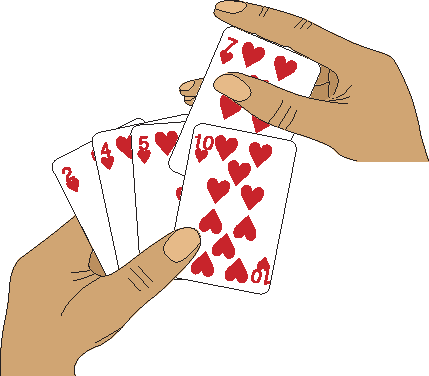
\includegraphics{算法导论第四版插图/第二章/插入排序打牌示意图.pdf}
    \caption{使用插入排序对手中的牌进行排序}
    \label{fig:使用插入排序对手中的牌进行排序}
\end{figure}

下面是插入排序的伪代码,称为INSERTION-SORT过程。它有两个参数:一个包含要排序的值的数组$A$和要排序的值的数量$n$。这些值占据数组$A$的$A[1]$到$A[n]$位置,我们用$A[1:n]$表示。当INSERTION-SORT过程完成后,数组$A[1:n]$包含原始值,但是已按排序顺序排列。

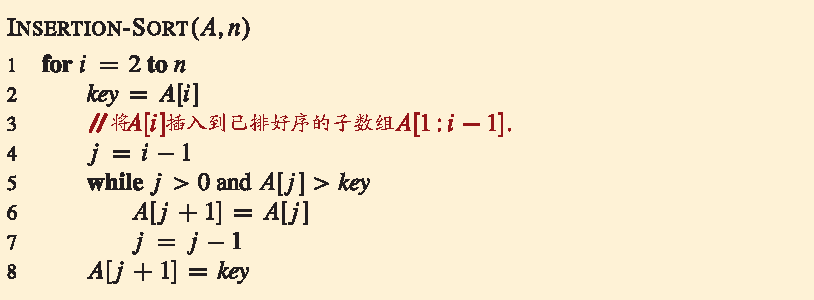
\includegraphics{算法导论第四版插图/第二章/插入排序伪代码.pdf}

\textbf{循环不变式和插入排序的正确性}

\begin{figure}[htbp]
    \centering
    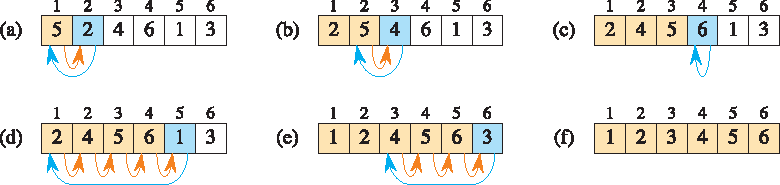
\includegraphics{算法导论第四版插图/第二章/插入排序过程示意图.pdf}
    \caption{INSERTION-SORT$(A,n)$的操作,其中$A$最初包含序列$\langle 5,2,4,6,1,3 \rangle$以及有$n = 6$。数组索引出现在矩形上方,数组位置中存储的值出现在矩形内部。(a)-(e) 行1-8的\textbf{for}循环迭代。在每次迭代中,蓝色矩形中存放着从$A[i]$中取出的$key$,该$key$与行5中其左边的棕色矩形中的值进行比较。橙色箭头显示在行6中向右移动一个位置的数组值,蓝色箭头指示$key$在行8中移动到的位置。(f) 最终排序的数组。}
    \label{fig:插入排序过程示意图}
\end{figure}

图\ref{fig:插入排序过程示意图}展示了该算法如何对初始序列$\langle 5,2,4,6,1,3\rangle$的数组$A$进行排序。索引$i$表示正在插入到手中的``当前卡片''。在每次由$i$索引的\textbf{for}循环的开始时,子数组(数组的连续部分)$A[1:i-1]$(即$A[1]$到$A[i-1]$)构成当前已排序的手牌,而剩余的子数组$A[i+1:n]$(元素$A[i+1]$到$A[n]$)对应于仍留在桌上的牌堆。实际上,元素$A[1:i-1]$是最初在位置1到$i-1$上的元素,但现在以排序顺序排列。我们将$A[1:i-1]$的这些属性正式陈述为一个循环不变式:

\begin{tcolorbox}
在第 1-8 行的 \textbf{for} 循环的每次迭代开始时,子数组 $A[1:i-1]$ 由原来在 $A[1:i-1]$ 中的元素组成,但已经按序排列。
\end{tcolorbox}

循环不变式主要用来帮助我们理解算法的正确性。关于循环不变式,我们必须证明三条性质:

\textbf{初始化}:循环的第一次迭代之前,循环不变式为真。

\textbf{保持}:如果循环的某次迭代之前循环不变式为真,那么下次迭代之前循环不变式仍为真。

\textbf{终止}:在循环终止时,循环不变式(通常会包含循环终止的原因)为我们提供一个有用的性质,该性质有助于证明算法是正确的。

当前两条性质成立时,在循环的每次迭代之前循环不变式为真。(当然,为了证明循环不变式在每次迭代之前保持为真,我们完全可以使用不同于循环不变式本身的其他已证实的事实。)注意,这类似于数学归纳法,其中为了证明某条性质成立,需要证明一个基本情况和一个归纳步骤。这里,证明第一次迭代之前循环不变式成立对应于基本情况,证明从一次迭代到下一次迭代不变式成立对应于归纳步骤。

第三条性质也许是最重要的,因为我们将使用循环不变式来证明正确性。通常,我们和导致循环终止的条件一起使用循环不变式。终止性不同于我们通常使用数学归纳法的做法,在归纳法中,归纳步骤是无限地使用的,这里当循环终止时,停止``归纳''。

让我们看看对于插入排序,如何证明这些性质成立。

\textbf{初始化}:首先证明在第一次循环迭代之前(当$i=2$时),循环不变式成立。所以子数组$A[1:i-1]$仅由单个元素$A[1]$组成,实际上就是$A[1]$中原来的元素。而且该子数组是排序好的(毕竟,只包含一个元素的子数组怎么样才不是已经排好序的呢?)。这表明第一次循环迭代之前循环不变式成立。

\textbf{保持}:其次处理第二条性质:证明每次迭代保持循环不变式。非形式化地, \textbf{for} 循环体的第 4-7 行将 $A[i-1]$、$A[i-2]$、$A[i-3]$等向右移动一个位置,直到找到 $A[i]$ 的适当位置,第 8 行将 $A[i]$ 的值插入该位置。这时子数组 $A[1:i]$ 由原来在 $A[1:i]$ 中的元素组成,但已按序排列。那么对 \textbf{for} 循环的下一次迭代增加$i$将保持循环不变式。

第二条性质的一种更形式化的处理要求我们对第 5-7 行的 \textbf{while} 循环给出并证明一个循环不变式。然而,这里我们不愿陷入形式主义的困境,而是依赖以上非形式化的分析来证明第二条性质对外层循环成立。

\textbf{终止}:最后研究在循环终止时发生了什么。循环变量$i$从2开始,每次迭代增加1。一旦第1行代码的$i$的值超过了$n$,循环就将终止。也就是循环会在$i=n+1$时终止。在循环不变式的表述中将$i$用$n+1$代替,我们有:子数组 $A[1:n]$ 由原来在 $A[1:n]$ 中的元素组成,但已按序排列。注意到,子数组 $A[1:n]$ 就是整个数组,我们推断出整个数组已排序。因此算法正确。

在本章后面以及其他章中,我们将采用这种循环不变式的方法来证明算法的正确性。

\textbf{伪代码中的一些约定}

\begin{itemize}
    \item 缩进表示块结构。例如,第 1 行开始的 \textbf{for} 循环体由第 2-8 行组成,第 5 行开始的 \textbf{while} 循环体包含第 6-7 行但不包含第 8 行。我们的缩进风格也适用于 \textbf{if-else} 语句。采用缩进来代替常规的块结构标志,如 \textbf{begin} 和 \textbf{end} 语句,可以大大提高代码的清晰性。
    \item \textbf{while}、\textbf{for} 与 \textbf{repeat-until} 等循环结构以及 \textbf{if-else} 等条件结构与C、C++、Java、Python和JavaScript中的那些结构具有类似的解释。不像某些出现于C++、Java和JavaScript中的情况,本书中在退出循环后,循环计数器保持其值。因此,紧接在一个 \textbf{for} 循环后,循环计数器的值就是第一个超出 \textbf{for} 循环界限的那个值。在证明插入排序的正确性时,我们使用了该性质。第 1 行的 \textbf{for} 循环头为 \textbf{for} $i=2$ \textbf{to} $n$,所以,当该循环终止时,$i=n+1$。当一个 \textbf{for} 循环每次迭代增加其循环计数器时,我们使用关键词\textbf{to}。当一个\textbf{for}循环每次迭代减少其循环计数器时,我们使用关键词 \textbf{downto} 。当循环计数器以大于 1 的一个量改变时,该改变量跟在可选关键词 \textbf{by} 之后。
    \item 符号``//''表示该行后面部分是个注释。
    \item 变量(例如$i$,$j$和$key$)都是给定过程的局部变量。我们在不明确说明的情况下,不使用全局变量。
    \item 我们通过在方括号中指定数组名后跟索引来访问数组元素。例如,$A[i]$表示数组$A$的第$i$个元素。

    尽管许多编程语言对数组采用从0开始的索引(0是最小有效索引),但我们选择最清晰易懂的索引方案供人类读者理解。因为人们通常从1开始计数,而不是从0开始,所以本书中的大多数(但不是全部)数组使用从1开始的索引。为了明确一个特定算法是基于0索引还是1索引,我们会明确指定数组的边界。如果你正在使用一个伪代码算法,是从1开始的索引,但你正在使用数组从0开始索引的编程语言(如C、C++、Java、Python或JavaScript)编写代码,那么将伪代码转换成代码应该不成问题。你可以选择始终从每个索引中减去1,或者为每个数组分配一个额外的位置,并忽略索引0。

    符号``:''表示子数组。因此,$A[i:j]$表示由元素$A[i],A[i+1],\cdots,A[j]$组成的$A$的子数组。我们还使用这个符号来表示数组的边界,就像我们之前讨论数组$A[1:n]$时所做的那样。
    \item 通常,我们将复合数据组织成对象,对象由属性组成。我们使用许多面向对象编程语言中的语法来访问特定的属性:对象名称,后跟一个点,再后跟属性名称。例如,如果一个对象$x$具有属性$f$,我们用$x.f$表示该属性。

    我们将表示数组或对象的变量视为指向表示数组或对象的数据的指针(在某些编程语言中称为引用)。对于对象$x$的所有属性$f$,将$y = x$设置后,$y.f$将等于$x.f$。此外,如果我们现在设置$x.f = 3$,那么之后不仅$x.f$等于3,$y.f$也等于3。换句话说,在赋值$y = x$之后,$x$和$y$指向同一个对象。这种处理数组和对象的方式与大多数现代编程语言一致。

    我们的属性表示法可以``级联''。例如,假设属性$f$本身是指向某种具有属性$g$的对象的指针。那么表示法$x.f.g$隐式地被表示为$(x.f).g$。换句话说,如果我们已经将$y = x.f$赋值,那么$x.f.g$和$y.g$是相同的。

    有时指针可能不指向任何对象。在这种情况下,我们给它一个特殊的值NIL。
    \item 我们通过\textbf{值传递}方式将参数传递给过程:被调用的过程接收到的是实际参数的副本,如果被调用过程对参数进行赋值,调用过程不会看到这个变化。当对象被传递时,表示对象的数据的指针被复制,但对象的属性不会被复制。例如,如果$x$是一个被调用过程的参数,被调用过程中的赋值操作$x=y$对调用过程是不可见的。然而,如果调用过程与$x$指向同一个对象,则赋值操作$x.f=3$是可见的。类似地,数组是通过指针传递的,因此传递的是指向数组的指针而不是整个数组,对单个数组元素的更改对调用过程是可见的。再次强调,大多数当代编程语言都是以这种方式工作的。
    \item \textbf{return}语句立即将控制权转回调用过程中的调用点。大多数\textbf{return}语句还接受一个值作为返回给调用者的结果。我们的伪代码与许多编程语言不同之处在于,我们允许在单个\textbf{return}语句中返回多个值,而不需要创建对象将它们打包在一起。
    \item 布尔运算符``and''和``or''具有短路求值的特性。也就是说,对于表达式``$x$ and $y$'',首先求值$x$。如果$x$的值为FALSE,则整个表达式无法为TRUE,因此不会对$y$进行求值。另一方面,如果$x$的值为TRUE,则必须对$y$进行求值以确定整个表达式的值。类似地,在表达式``$x$ or $y$''中,只有当$x$的值为FALSE时才会对$y$进行求值。短路求值的运算符使我们能够编写布尔表达式,例如``$x$ != NIL and $x.f=y$'',而无需担心当$x$为NIL时对``$x.f$''的求值会发生什么。
    \item 关键字\textbf{error}表示发生了错误,因为调用过程的条件不满足,所以过程立即终止。调用过程负责处理错误,因此我们不指定要采取的具体操作。
\end{itemize}

\section{分析算法}\label{section-2.2}

分析算法的含义已经演变为预测算法所需的资源。你可能考虑到的资源包括内存、通信带宽或能量消耗。然而,最常见的情况是你会希望衡量算法的运行时间。如果你分析一个问题的多个候选算法,你可以找出最高效的算法。可能会有不止一个可行的候选算法,但在这个过程中通常可以排除一些较差的算法。

在你分析算法之前,你需要一个运行算法的技术模型,包括技术模型的资源以及一种表示算法执行成本的方法。本书的大部分内容假设计算机程序的实现技术是通用的单处理器随机访问机(RAM)模型,同时假设算法以计算机程序的形式实现。在RAM模型中,指令一条接一条地执行,没有并发操作。RAM模型假设每条指令的执行时间与其他指令相同,并且每次数据访问(使用变量的值或将值存储到变量中)的时间与其他数据访问相同。换句话说,在RAM模型中,每条指令或数据访问都需要固定的时间,即使是对数组的索引操作也是如此。

严格来说,我们应该准确地定义RAM模型中的指令及其成本。然而,这样做将变得冗长,并且对算法设计和分析的洞察力帮助不大。然而,我们必须小心不要滥用RAM模型。例如,如果RAM模型中有一个排序的指令,那么你可以一步就完成排序操作。这样的RAM是不现实的,因为真实计算机中不存在这样的指令。因此,我们的技术模型的来源是真实计算机的设计方式。RAM模型包含在真实计算机中常见的指令:算术运算(如加法、减法、乘法、除法、取余、向下取整、向上取整)、数据移动(加载、存储、复制)和控制流(条件和无条件分支、子程序调用和返回)。

RAM模型中的数据类型包括整数、浮点数(用于存储实数近似值)和字符。真实计算机通常没有单独的数据类型来表示布尔值TRUE和FALSE。相反,它们经常测试一个整数值是否为0(FALSE)或非零(TRUE),就像在C语言中一样。尽管在本书中我们通常不关心浮点数的精度(许多数值在浮点数中无法精确表示),但对于大多数应用程序来说,精度至关重要。我们还假设每个数据字的位数有一个限制。例如,在处理大小为$n$的输入时,我们通常假设整数由$c\log 2n$位表示,其中$c \ge 1$为某个常数。我们要求$c \ge 1$以便每个字可以容纳$n$的值,使我们能够索引各个输入元素,并限制$c$为一个常数,以避免字大小任意增长。(如果字大小可以任意增长,我们可以在一个字中存储大量数据,并在常数时间内对其进行操作,这是一个不现实的场景。)

实际计算机包含未在上述列表中列出的指令,这些指令在RAM模型中代表了一个灰色区域。例如,指数运算是否是一个常数时间的指令?一般情况下,不是的:计算$x^n$,其中$x$和$n$是一般整数,通常需要时间与$n$的对数成比例,而且你必须担心结果是否能存储在计算机字中(而不会发生溢出)。然而,如果$n$是一个精确的2的幂,指数运算通常可以视为一个常数时间的操作。许多计算机具有``左移''指令,该指令在常数时间内将整数的位向左移动$n$位。在大多数计算机中,将整数的位左移1位等同于乘以2,因此将位左移$n$位等同于乘以$2^n$。因此,只要$n$不超过计算机字的位数,这些计算机可以通过将整数1左移$n$位来在1个常数时间指令内计算$2^n$。我们将尽量避免RAM模型中的这种灰色区域,并将计算$2^n$和乘以$2^n$视为常数时间的操作,前提是结果足够小且能保存在计算机字中。

RAM模型没有考虑到在当代计算机中普遍存在的内存层次结构。它既没有模拟缓存,也没有模拟虚拟内存。几种其他计算模型试图考虑内存层次效应,这在实际机器上的真实程序中有时非常重要。本书的第\ref{section-11.5}节和一些问题考察了内存层次效应,但在大部分情况下,本书的分析并不考虑这些效应。包含内存层次结构的模型比RAM模型复杂得多,因此使用起来可能会很困难。此外,RAM模型的分析通常对实际机器上的性能预测非常准确。

虽然通常在RAM模型中分析算法是直接的,但有时也可能很具有挑战性。你可能需要运用数学工具,如组合数学、概率论、一些代数技巧以及识别公式中最重要项的能力。因为算法可能对每个可能的输入表现不同,我们需要一种方式来用简单易懂的公式总结其行为。

\textbf{插入排序的分析}

插入排序(INSERTION-SORT)过程需要多长时间?一种方法是在你的计算机上运行它并统计运行时间。当然,你首先需要用一种真实的编程语言实现它,因为无法直接运行我们的伪代码。这样的计时测试会告诉你什么?你将了解插入排序在你这台特定的计算机上、特定的输入下、你编写的特定算法实现中、你运行的特定编译器或解释器、你链接的特定的库以及与你的计时测试同时运行的特定的一些后台任务(例如检查网络上的传入信息)下运行所需的时间。如果你再次在相同的输入上在你的计算机上运行插入排序,你甚至可能得到不同的计时结果。从仅在一个计算机上的一种插入排序实现以及一个输入上运行,如果你给它一个不同的输入、在不同的计算机上运行它,或者用不同的编程语言实现它,你能确定有关插入排序运行时间的什么呢?能得到的信息并不多。我们需要一种预测的方法,能够根据新的输入来预测插入排序所需的时间。

与其计时运行插入排序,甚至进行多次运行,我们可以通过分析算法本身来确定所需时间。我们将研究算法执行每一行伪代码的次数以及每行伪代码的运行时间。我们首先会得出一个精确但复杂的运行时间公式。然后,我们将使用一种方便的符号表示法,提取公式的重要部分,以便对解决同一问题的不同算法的运行时间进行比较。

我们如何分析插入排序?首先,我们知道运行时间取决于输入规模。排序1000个数字所需的时间比排序3个数字所需的时间长,并不令人感到惊讶。此外,相同大小的两个输入数组的插入排序可能需要不同的时间,这取决于输入数据已经排好序的程度。尽管运行时间可能取决于输入的许多特征,但我们将重点关注已被证明具有最大影响的特征,即输入规模的大小,并将程序的运行时间描述为输入规模大小的函数。为此,我们需要更仔细地定义``运行时间''和``输入规模大小''这些术语。我们还需要明确我们是在讨论引发最坏情况、最好情况还是其他情况下的运行时间。

输入规模大小的最佳概念取决于所研究的问题。对于许多问题,例如排序或计算离散傅里叶变换,最自然的度量方式是输入中项的数量——例如,正在排序的项的数量$n$。对于许多其他问题,例如两个整数的乘法,输入大小的最佳度量是表示输入所需的总位数(采用普通二进制表示法)。有时,用一个以上的数描述输入的大小更加合适。例如,如果算法的输入是一个图数据结构,通常通过图的顶点的数量和边的数量来表征输入的大小。我们将在研究的每个问题中指明使用的输入大小的度量方式。

算法在特定输入上的运行时间是执行指令的次数和数据访问的次数。我们计算这些开销的方法应该独立于任何特定计算机,而在RAM模型的框架内进行。我们暂时采用以下观点。执行伪代码的每一行都需要常数时间。某一行伪代码可能比另一行伪代码需要更多或更少的时间,但我们假设第$k$行的每次执行都需要$c_k$的时间,其中$c_k$是一个常数。这个观点与RAM模型一致,也反映了伪代码在大多数实际计算机上的实现方式。

让我们分析插入排序过程。如前所述,我们将首先设计一个精确的公式,其中使用了输入大小和所有语句的成本$c_k$。然而,这个公式看起来可能会比较复杂。然后,我们将切换到一种更简洁、更易于使用的简化符号表示法。这种简化表示法清楚地说明了如何比较算法的运行时间,特别是随着输入大小的增加。

为了分析INSERTION-SORT过程,下面的插入排序程序记录了每个语句的时间成本和每个语句的执行次数。对于每个$i=2,3,\cdots,n$,设$t_i$表示在第5行的\textbf{while}循环测试中对于该$i$值执行的次数。当\textbf{for}循环或\textbf{while}循环以常见的方式退出(在循环头中的测试结果为FALSE时,循环退出),测试的执行次数比循环体多1次。由于注释不是可执行语句,假设它们不占用时间。

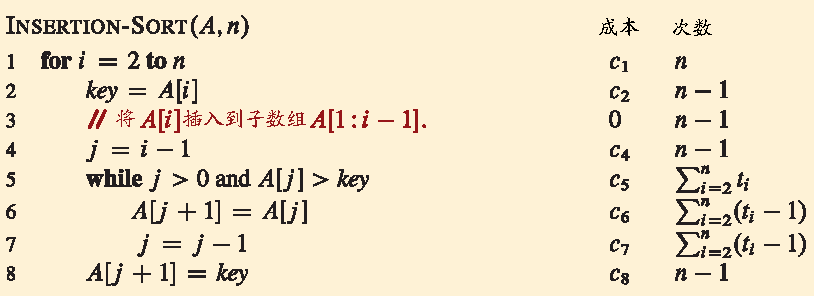
\includegraphics{算法导论第四版插图/第二章/插入排序时间复杂度的代码.pdf}

算法的运行时间是每个语句执行时间的总和。执行需要$c_k$条指令并且执行$m$次的一行伪代码对总运行时间的贡献为$c_km$。我们通常用$T(n)$表示算法在大小为$n$的输入上的运行时间。要计算$T(n)$,即INSERTION-SORT在给定输入值上的运行时间,我们将成本和次数两列的乘积相加,得到

\begin{equation*}
\begin{aligned}
T(n)= & c_1 n+c_2(n-1)+c_4(n-1)+c_5 \sum_{i=2}^n t_i+c_6 \sum_{i=2}^n(t_i-1) \\
& +c_7 \sum_{i=2}^n(t_i-1)+c_8(n-1)
\end{aligned}
\end{equation*}

即使对于给定大小的输入,算法的运行时间可能取决于给定的该大小的输入。例如,在INSERTION-SORT中,最佳情况是数组已经排序好。在这种情况下,每次执行第5行时,$key$的值(即最初在$A[i]$中的值)已经大于或等于$A[1:i-1]$中的所有值,因此在第5行的第1次测试中,循环将总是退出。因此,我们有$t_i=1$对于$i=2,3,\cdots,n$,最佳情况的运行时间由以下公式给出

\begin{equation}\label{eq:2.1}
\begin{aligned}
T(n) & =c_1 n+c_2(n-1)+c_4(n-1)+c_5(n-1)+c_8(n-1) \\
& =(c_1+c_2+c_4+c_5+c_8)n-(c_2+c_4+c_5+c_8)
\end{aligned}
\end{equation}

我们可以将这个运行时间表示为$an+b$,其中$a$和$b$是依赖于语句成本$c_k$的常数(其中$a = c_1 + c_2 + c_4 + c_5 + c_8$,$b = c_2 + c_4 + c_5 + c_8$)。因此,运行时间是$n$的线性函数。

最坏情况出现在数组按逆序排列的情况下,即初始时按降序排列。该过程必须将每个元素$A[i]$与整个已排序子数组$A[1:i-1]$中的每个元素进行比较,因此对于$i=2,3,\cdots,n$,$t_i = i$。(在第5行,该过程发现每次$A[j] > key$,并且\textbf{while}循环仅在$j$达到0时退出。)注意到

\begin{equation*}
\begin{aligned}
\sum_{i=2}^n i & =(\sum_{i=1}^n i)-1 \\
& =\frac{n(n+1)}{2}-1
\end{aligned}
\end{equation*}

和

\begin{equation*}
\begin{aligned}
\sum_{i=2}^n(i-1) & =\sum_{i=1}^{n-1} i \\
& =\frac{n(n-1)}{2}
\end{aligned}
\end{equation*}

我们可以看到插入排序在最坏情况下的运行时间是

\begin{equation}\label{eq:2.2}
\begin{aligned}
T(n)= & c_1 n+c_2(n-1)+c_4(n-1)+c_5(\frac{n(n+1)}{2}-1) \\
& +c_6(\frac{n(n-1)}{2})+c_7(\frac{n(n-1)}{2})+c_8(n-1) \\
= & (\frac{c_5}{2}+\frac{c_6}{2}+\frac{c_7}{2}) n^2+(c_1+c_2+c_4+\frac{c_5}{2}-\frac{c_6}{2}-\frac{c_7}{2}+c_8) n \\
& -(c_2+c_4+c_5+c_8)
\end{aligned}
\end{equation}

我们可以将最坏情况的运行时间表示为$an^2+bn+c$,常数$a$,$b$和$c$依赖于语句代价$c_k$(现在,$a=c_5 / 2+c_6 / 2+c_7 / 2$,$b=c_1+c_2+c_4+c_5 / 2-c_6 / 2-c_7 / 2+c_8$以及($c=-(c_2+c_4+c_5+c_8)$)。这个运行时间是$n$的平方函数(二次函数)。

一般来说,对于给定输入,插入排序的运行时间是固定的,尽管我们可能会看到某些有趣的``随机''算法,对于这些算法而言,对于固定的输入,算法的行为可能会变化。

\textbf{最坏情况和平均情况的分析}

我们对插入排序的分析同时考虑了最好情况(即输入数组已经排序)和最坏情况(即输入数组按逆序排列)。然而,在本书的剩余部分,我们通常(但不总是)只关注寻找最坏情况的运行时间,即任意大小为$n$的输入的最长运行时间。为什么呢?以下是三个原因:

\begin{itemize}
    \item 算法的最坏情况运行时间为任何输入提供了一个运行时间的上界。如果你知道最坏情况运行时间,那么你可以确保算法永远不会花费更长的时间。你不需要对运行时间进行猜测,并希望它不会变得更糟。这一特性对于实时计算尤其重要,因为在实时计算中,操作必须在截止日期之前完成。
    \item 对于某些算法,最坏情况经常发生。例如,在搜索数据库中的特定信息时,搜索算法的最坏情况通常发生在数据库中不存在该信息的情况下。在某些应用中,对不存在信息的搜索可能很频繁。
    \item ``平均情况''通常与最坏情况差不多糟糕。假设你在一个包含 $n$ 个随机选择数字的数组上运行插入排序。确定将元素 $A[i]$ 插入子数组 $A[1:i-1]$ 中的位置需要多长时间?平均而言,$A[1:i-1]$ 的一半元素小于 $A[i]$,另一半元素大于 $A[i]$。因此,平均而言,$A[i]$ 与子数组 $A[1:i-1]$ 的一半元素进行比较,所以$t_i$大约为$i/2$。因此,结果的平均情况运行时间是输入规模的二次函数,就像最坏情况运行时间一样。
\end{itemize}

在某些特定情况下,我们对算法的平均情况运行时间感兴趣。我们将在本书中看到概率分析技术应用于各种算法。平均情况分析的范围有限,因为对于特定问题的``平均''输入可能不明确。通常,我们假设给定大小的所有输入等可能出现。实际上,这个假设可能被违反,但我们有时可以使用随机化算法,通过进行随机选择来进行概率分析并得出预期的运行时间。我们在第\ref{chapter-05}章和其他几个后续章节中更详细地探讨随机化算法。

\textbf{增长量级}

为了简化对INSERTION-SORT过程的分析,我们使用了一些简化的抽象概念。首先,我们忽略了每个语句的实际成本,而使用常数$c_k$来表示这些成本。然而,等式\eqref{eq:2.1}和\eqref{eq:2.2}中的最佳情况和最坏情况的运行时间相当复杂。这些表达式中的常数提供了比我们实际需要的更多细节。这就是为什么我们还将最佳情况的运行时间表示为$an+b$,其中$a$和$b$是依赖于语句成本$c_k$的常数,以及为什么我们将最坏情况的运行时间表示为$an^2+bn+c$,其中$a$,$b$和$c$是依赖于语句成本的常数。因此,我们不仅忽略了实际的语句成本,还忽略了抽象的成本$c_k$。

现在让我们再做一个简化的抽象:我们真正关心的是运行时间的增长率或阶数。因此,我们只考虑公式的主要项(例如,$an^2$),因为对于较大的$n$值来说,次要项相对不重要。我们还忽略主要项的常数系数,因为对于较大的输入,常数因子不如增长率在确定运行时间时重要。对于插入排序的最坏情况运行时间,当我们忽略次要项和主要项的常数系数时,只剩下主要项的$n^2$因子。这个因子$n^2$是运行时间中最重要的部分。例如,假设一个算法在特定机器上在大小为$n$的输入上花费$n^2/100 + 100n + 17$微秒。尽管$n^2$项的系数$1/100$和$n$项的系数100相差了四个数量级,但是一旦$n$超过10000,$n^2/100$项就主导了$100n$项。尽管10000可能看起来很大,但它比一个普通城镇的人口要小。许多现实世界的问题具有更大的输入规模。

为了突出运行时间的增长率,我们使用了特殊的符号,使用希腊字母$\Theta$(theta)。我们表示插入排序的最坏情况运行时间为$\Theta(n^2)$。我们还表示插入排序的最好情况运行时间为$\Theta(n)$。暂时将$\Theta$表示法视为表示``当$n$很大时大致成正比''的方式,因此$\Theta(n^2)$表示``当$n$很大时大致与$n^2$成正比'',$\Theta(n)$表示``当$n$很大时大致与$n$成正比''。我们将在本章中非正式地使用$\Theta$记号,并在第\ref{chapter-03}章中精确定义它。

通常情况下,如果一个算法的最坏情况运行时间具有较低的增长阶数,我们会认为该算法比另一个算法更高效。由于常数因子和次要项的影响,具有较高增长阶数的算法在小规模输入上可能比具有较低增长阶数的算法花费更少的时间。但是在足够大的输入上,一个最坏情况运行时间为$\Theta(n^2)$的算法,例如,其最坏情况下的运行时间比一个最坏情况运行时间为$\Theta(n^3)$的算法更少。无论$\Theta$表示法中隐藏了哪些常数,总是存在某个数$n_0$,使得对于所有输入大小$n\ge n_0$,$\Theta(n^2)$算法在最坏情况下击败$\Theta(n^3)$算法。

\section{设计算法}\label{section-2.3}

你可以选择从广泛的算法设计技术中进行选择。插入排序使用增量方法:对于每个元素$A[i]$,将其插入到子数组$A[1:i]$的适当位置,而子数组$A[1:i-1]$是已经排好序的。

本节介绍了另一种设计方法,称为``分治法'',我们将在第\ref{chapter-04}章中详细探讨。我们将使用分治法设计一个排序算法,其最坏情况运行时间远远小于插入排序。使用遵循分治法的算法的一个优点是,分析其运行时间通常是直接的,使用的技术我们将在第\ref{chapter-04}章中探讨。

\subsection{分治策略}\label{subsection-2.3.1}

许多有用的算法都具有递归的结构:为了解决一个给定的问题,它们会递归(调用自身)一次或多次来处理紧密相关的子问题。这些算法通常遵循分治法:它们将问题分解为几个与原始问题类似但规模较小的子问题,递归地解决这些子问题,然后将这些子问题的解合并来得到原始问题的解。

在分治法中,如果问题足够小(基本情况),则直接解决它而不进行递归。否则(递归情况),你执行三个特定的步骤:

\textbf{分解}原问题为若干子问题,这些子问题是原问题的规模较小的实例。

\textbf{解决}这些子问题,递归地求解各子问题。然而,若子问题的规模足够小,则直接求解。

\textbf{合并}这些子问题的解成原问题的解。

\textbf{归并排序}算法严格遵照了以上的分治策略。在每一个步骤,归并排序会对子数组$A[p:r]$进行排序。归并排序从整个数组$A[1:n]$开始,一直递归下降到越来越小的子数组。下面就是归并排序的操作过程:

\textbf{分解}:将待排序的子数组 $A[p:r]$ 分成两个相邻的子数组,每个子数组的大小都是原数组的一半。为此,计算子数组 $A[p:r]$ 的中点 $q$(取 $p$ 和 $r$ 的平均值),并将 $A[p:r]$ 分成子数组 $A[p:q]$ 和 $A[q+1:r]$。

\textbf{解决}:通过使用归并排序对两个子数组 $A[p:q]$ 和 $A[q+1:r]$ 进行递归排序来解决子数组的排序问题。

\textbf{合并}:通过将两个已排序的子数组 $A[p:q]$ 和 $A[q+1:r]$ 合并回 $A[p:r]$,得到排序好的答案。

当待排序的子数组 $A[p:r]$ 仅包含1个元素时,即 $p$ 等于 $r$ 时,递归``沉底''(到达基本情况)。正如我们在INSERTION-SORT循环不变式的初始化参数中指出的那样,只包含一个元素的子数组总是有序的。

归并排序算法的关键操作发生在``合并''步骤中,即合并两个相邻的已排序子数组。合并操作是由下面给出的辅助过程 MERGE$(A,p,q,r)$ 执行的,其中 $A$ 是一个数组,$p$、$q$ 和 $r$ 是数组的索引,满足 $p\le q < r$。该过程假设相邻的子数组 $A[p:q]$ 和 $A[q+1:r]$ 已经递归地排序好了。它将这两个已排序的子数组合并成一个单独的已排序子数组,取代当前的子数组 $A[p:r]$。

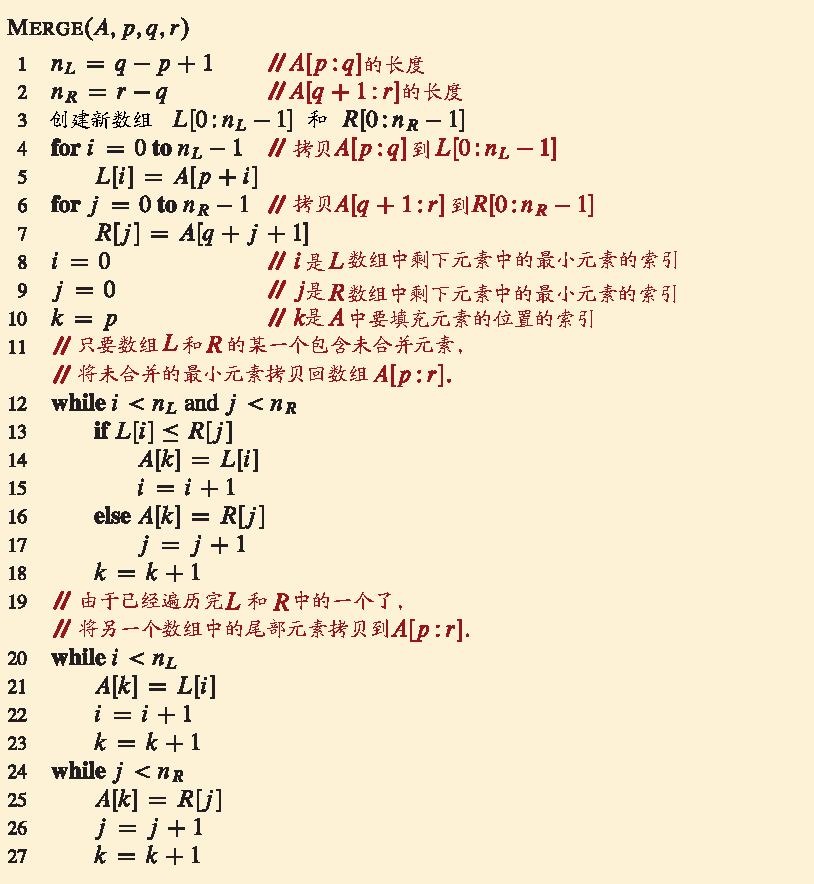
\includegraphics{算法导论第四版插图/第二章/归并过程伪代码.pdf}

为了理解MERGE过程的工作原理,让我们回到我们之前提到的纸牌游戏的情景。假设你在桌子上有两堆面朝上的纸牌。每堆纸牌都是有序的,最小值的牌在顶部。你希望将这两堆纸牌合并成一堆有序的纸牌,放在桌子上面朝下。基本步骤包括选择两堆面朝上纸牌中较小的一张牌,将其从所属的堆中移除(暴露出新的顶部牌),然后将这张牌面朝下放在输出堆上。重复这个步骤,直到其中一堆纸牌为空,这时你可以将剩下的一堆纸牌整体翻转并放在输出堆上。

我们来思考一下合并两堆有序纸牌需要多长时间。每个基本步骤都需要固定的时间,因为你只是比较两张顶部的纸牌。如果你开始时的两堆有序纸牌分别有$n/2$张牌,那么基本步骤的数量至少为$n/2$(因为在其中一堆被清空时,每张纸牌都被发现比另一堆的某张纸牌小),最多为$n$(实际上最多为$n-1$,因为经过$n-1$个基本步骤后,其中一堆必定为空)。每个基本步骤花费固定的时间,而总的基本步骤数量在$n/2$和$n$之间,因此我们可以说合并操作的时间与$n$大致成正比。也就是说,合并操作的时间复杂度为$\Theta(n)$。

具体来说,MERGE过程的工作步骤如下。它将两个子数组$A[p:q]$和$A[q+1:r]$复制到临时数组$L$和$R$(``Left''和``Right''),然后将$L$和$R$中的值合并回$A[p:r]$中。第1行和第2行计算子数组$A[p:q]$和$A[q+1:r]$的长度$n_L$和$n_R$,然后第3行创建具有长度$n_L$和$n_R$的数组$L[0:n_L-1]$和$R[0:n_R-1]$。第4至第5行的\textbf{for}循环将子数组$A[p:q]$复制到$L$,第6至第7行的\textbf{for}循环将子数组$A[q+1:r]$复制到$R$。

\begin{figure}[htbp]
    \centering
    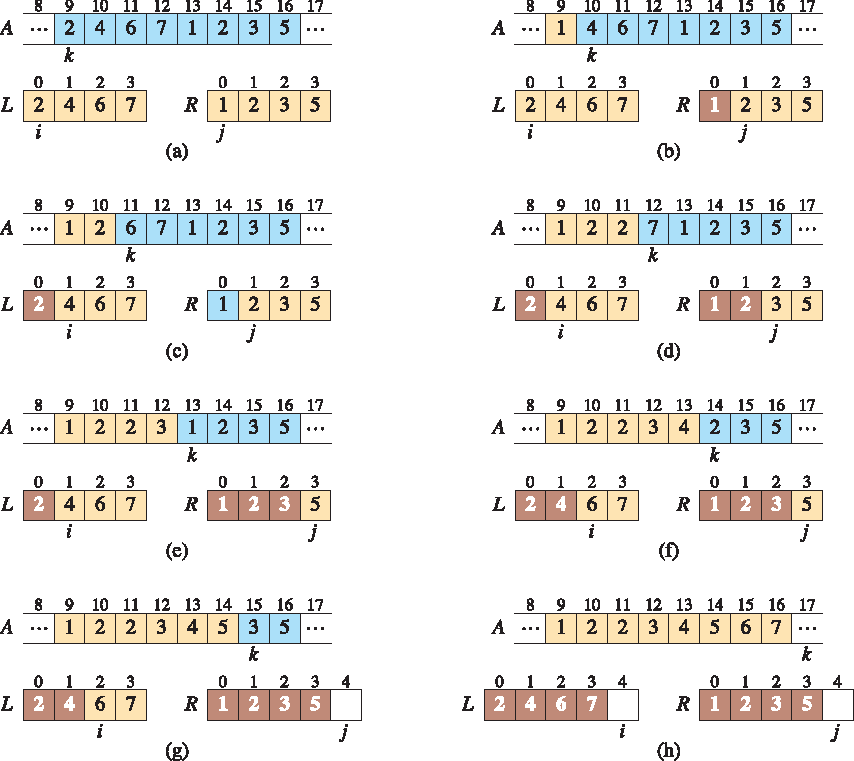
\includegraphics{算法导论第四版插图/第二章/归并过程示意图.pdf}
    \caption{在调用MERGE$(A,9,12,16)$时,循环行8-18中的操作是,当子数组$A[9:16]$包含值$\langle 2,4,6,7,1,2,3,5 \rangle$时进行的。在分配和复制到数组$L$和$R$之后,数组$L$包含$\langle 2,4,6,7 \rangle$,数组$R$包含$\langle 1,2,3,5 \rangle$。$A$中的棕色位置包含它们的最终值,$L$和$R$中的棕色位置包含尚未复制回$A$的值。总体而言,棕色位置始终包含最初在$A[9:16]$中的值。$A$中的蓝色位置包含将要复制的值,$L$和$R$中的深色位置包含已经复制回$A$的值。 (a)-(g)是循环12-18行的每次迭代之前的数组$A$、$L$和$R$以及它们的相应索引$k$、$i$和$j$。在(g)部分,$R$中的所有值都已经复制回$A$($j$等于$R$的长度),因此循环12-18行的\textbf{while}循环终止。(h)是终止时的数组和索引。行20-23的\textbf{while}循环复制回$A$中剩余的$L$和$R$的值,这些值是最初在$A[9:16]$中的最大值。在这里,行20-23将$L[2:3]$复制到$A[15:16]$,并且因为$R$中的所有值已经复制回$A$,所以循环24-27行的\textbf{while}循环迭代0次。此时,$A[9:16]$的子数组已经排序完成。}
    \label{fig:归并过程示意图}
\end{figure}

在图\ref{fig:归并过程示意图}中展示的第8-18行执行基本步骤。循环12-18行重复地在$L$和$R$中找到尚未复制回$A[p:r]$的最小值,并将其复制回去。正如注释所示,索引$k$表示正在填充的$A$的位置,索引$i$和$j$分别表示$L$和$R$中剩余最小值的位置。最终,$L$或$R$中的所有值都被复制回$A[p:r]$,并且此循环终止。如果循环终止是因为已经将$R$的所有值复制回去,即$j$等于$n_R$,那么$i$仍然小于$n_L$,这意味着$L$的一些值尚未复制回去,而这些值是$L$和$R$中最大的值。在这种情况下,循环20-23行将$L$的这些剩余值复制到$A[p:r]$的最后几个位置。因为$j$等于$n_R$,所以循环24-27行的\textbf{while}循环不会执行。如果相反,循环12-18行终止是因为$i$等于$n_L$,则所有的$L$已经被复制回$A[p:r]$,而循环24-27行将$R$的剩余值复制回$A[p:r]$的末尾。

为了证明MERGE过程在$\Theta(n)$的时间内运行,其中$n=r-p-1$,观察到第1-3行和第8-10行每行都需要常数时间,而第4-7行的循环需要$\Theta(n_L+n_R)=\Theta(n)$的时间。要计算第12-18行、20-23行和24-27行的三个\textbf{while}循环的时间,观察到这些循环的每次迭代都将$L$或$R$中的一个值复制回$A$,并且每个值都只复制回$A$一次。因此,这三个循环总共进行了$n$次迭代。由于这三个循环的每次迭代都需要常数时间,所以在这三个循环中总共花费的时间是$\Theta(n)$。

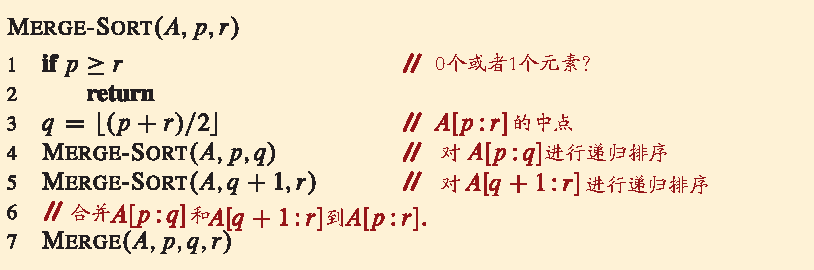
\includegraphics{算法导论第四版插图/第二章/归并排序主程序.pdf}

现在,我们可以将MERGE过程作为归并排序算法中的子程序使用。在过程MERGE-SORT$(A,p,r)$对子数组$A[p:r]$中的元素进行排序。如果$p$等于$r$,则子数组只有1个元素,因此已经排序。否则,我们必须有$p < r$,并且MERGE-SORT执行分解、解决和合并步骤。分解步骤简单地计算一个索引$q$,将$A[p:r]$分为两个相邻的子数组:$A[p:q]$,包含$\lceil{n/2}\rceil$个元素,和$A[q+1:r]$,包含$\lfloor{n/2}\rfloor$个元素。初始调用MERGE-SORT$(A,1,n)$对整个数组$A[1:n]$进行排序。

\begin{figure}[htbp]
    \centering
    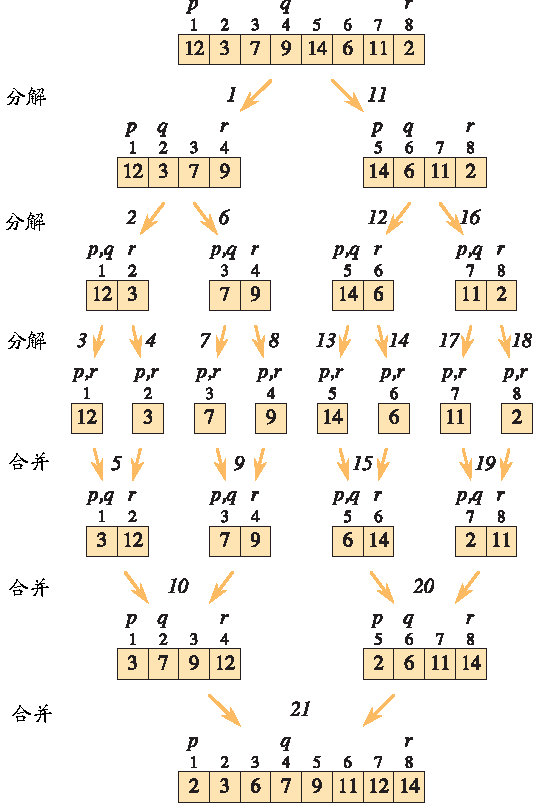
\includegraphics{算法导论第四版插图/第二章/归并排序完整过程示意图.pdf}
    \caption{归并排序在数组长度为8的数组$A$上面的操作过程。数组$A$最开始时是:$\langle{12,3,7,9,14,6,11,2}\rangle$}。每个子数组中的索引$p$、$q$和$r$如图所示。斜体数字表示了MERGE-SORT和MERGE过程的调用顺序,初始调用是MERGE-SORT$(A,1,8)$
    \label{fig:归并排序完整过程示意图}
\end{figure}

图\ref{fig:归并排序完整过程示意图}展示了当$n=8$时该过程的操作,还显示了分解和合并步骤的顺序。该算法递归地将数组分解为包含一个元素的子数组。合并步骤将成对的1元素子数组合并为长度为2的已排序子数组,将它们合并为长度为4的已排序子数组,最终将它们合并为长度为8的最终已排序子数组。如果$n$不是2的精确幂,则某些分割步骤会创建长度相差1的子数组(例如,将长度为7的子数组分割时,一个子数组长度为4,另一个子数组长度为3)。无论合并的两个子数组的长度如何,合并$n$个项的时间复杂度为$\Theta(n)$。

\subsection{分析分治算法}\label{subsection-2.3.2}

当一个算法包含递归调用时,通常可以通过\textbf{递归等式}或\textbf{递归式}来描述其运行时间,该递归方程描述了算法在较小输入上的运行时间与问题规模$n$上的总体运行时间之间的关系。然后,可以使用数学工具来解决递归方程并提供算法性能的界限。

分治算法的运行时间的递归方程可从基本方法的三个步骤中推导出来。与插入排序类似,假设$T(n)$是规模为$n$的问题的最坏情况运行时间。如果问题规模足够小,例如$n < n_0$,其中$n_0 > 0$是一个常数,直接的解只需要常数时间,我们将其表示为$\Theta(1)$。假设问题的划分产生了大小为$n/b$的子问题,即原问题大小的$1/b$。对于归并排序,$a$和$b$都是$2$,但是我们将看到其他分治算法中的$a\neq b$。解决一个大小为$n/b$的子问题需要$T(n/b)$的时间,因此解决所有$a$个子问题需要$aT(n/b)$的时间。如果将问题划分成子问题需要$D(n)$的时间,将子问题的解合并成原问题的解需要$C(n)$的时间,我们得到递归关系式

$$
T(n)= \begin{cases}\Theta(1) & \text { 如果 } n<n_0 \\ D(n)+a T(n / b)+C(n) & \text { 其他情况 }\end{cases}
$$

第\ref{chapter-04}章展示了如何求解以上形式的递归式。

有时候,分治算法中的划分步骤的大小 $n/b$ 不是整数。例如,归并排序将一个大小为 $n$ 的问题划分为大小为 $\lfloor{n/2}\rfloor$ 和 $\lceil{n/2}\rceil$ 的子问题。由于 $\lfloor{n/2}\rfloor$ 和 $\lceil{n/2}\rceil$ 之间的差异最多为 1,对于大的 $n$ 来说,这比将 $n$ 除以 2 的影响要小得多,因此我们会简单地将它们都称为大小为 $n/2$。正如第\ref{chapter-04}章所讨论的那样,忽略向上取整和向下取整运算并不会影响分治算法的递归式的解的增长量级。

我们还要采用的另一个约定是省略递归式的基本情况的语句,我们将在第\ref{chapter-04}章中更详细地讨论这个问题。原因是基本情况几乎总是$T(n)=\Theta(1)$,如果$n < n_0$,其中$n_0 > 0$是一个常数。这是因为算法在常量大小的输入上运行时间是常数的。采用这种约定可以节省大量的书写文档的时间。

\textbf{归并排序算法的分析}

下面是如何推导出归并排序在$n$个数字上的最坏情况运行时间$T(n)$的递归式:

\textbf{分解}:分解步骤只是计算子数组的中间位置,这需要常数时间。因此,$D(n)=\Theta(1)$。

\textbf{解决}:递归地解决两个大小为$n/2$的子问题,每个子问题对运行时间的贡献为$2T(n/2)$(忽略向下取整和向上取整)。

\textbf{合并}:由于对$n$元素子数组进行合并的MERGE过程需要$\Theta(n)$的时间,因此我们有$C(n)=\Theta(n)$。

当我们将归并排序分析中的函数 $D(n)$ 和 $C(n)$ 相加时,我们正在添加一个 $\Theta(n)$ 的函数和一个 $\Theta(1)$ 的函数。和是 $n$ 的线性函数。也就是说,当 $n$ 很大时,它大致与 $n$ 成正比,因此归并排序的分解和合并时间总共为 $\Theta(n)$。将 $\Theta(n)$ 添加到解决步骤中的 $2T(n/2)$ 项中,得到归并排序最坏情况运行时间 $T(n)$ 的递归式:

\begin{equation}\label{eq:2.3}
T(n)=2T(n/2)+\Theta(n)
\end{equation}

第\ref{chapter-04}章介绍了``主定理'',它表明$T(n)=\Theta(n\lg{n})$。与最坏情况运行时间为$\Theta(n^2)$的插入排序相比,归并排序以$n$的因子换取了$\lg n$的因子。因为对数函数增长比任何线性函数都要慢,所以这是一笔好买卖。对于足够大的输入,具有$\Theta(n \lg n)$最坏情况运行时间的归并排序优于最坏情况运行时间为$\Theta(n^2)$的插入排序。

我们不需要使用主定理来直观地理解为什么\eqref{eq:2.3}的递归解是$T(n) = \Theta(n \lg n)$。为简单起见,假设$n$是2的幂次方,隐含的基本情况是$n = 1$。那么递归式\eqref{eq:2.3}本质上是:

\begin{equation}\label{eq:2.4}
T(n)= \begin{cases}c_1 & \text { 如果 } n=1 \\ 2 T(n / 2)+c_2 n & \text { 如果 } n>1\end{cases}
\end{equation}

其中常数$c_1 > 0$表示解决大小为1的问题所需的时间,$c_2 > 0$是分解和合并步骤每个数组元素的时间。

\begin{figure}[htbp]
    \centering
    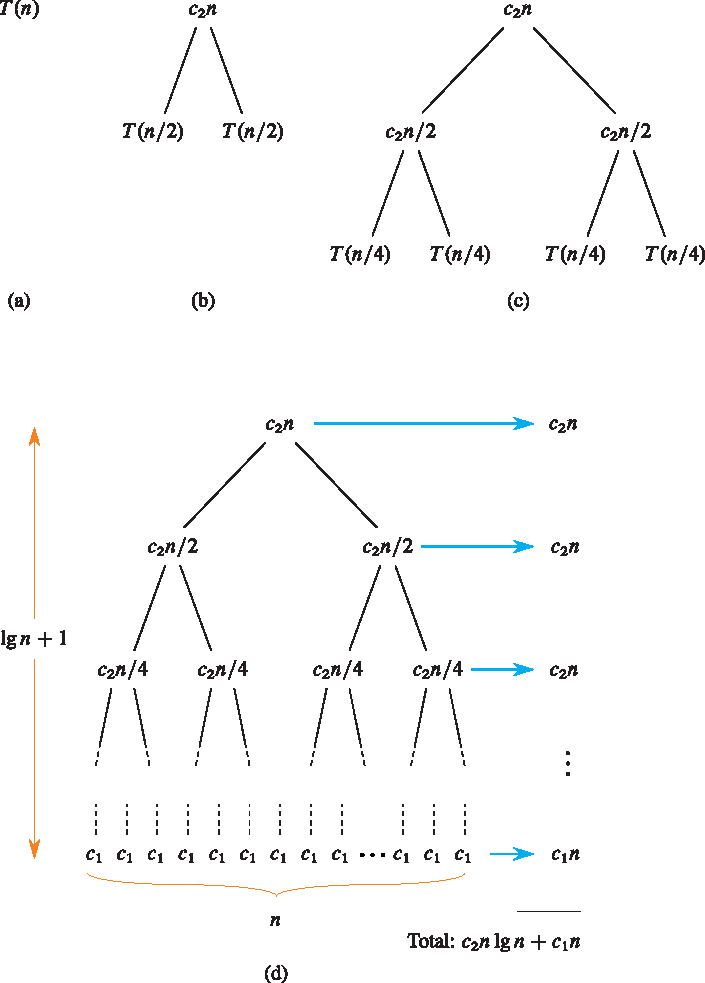
\includegraphics{算法导论第四版插图/第二章/归并排序的递归树示意图.pdf}
    \caption{如何为递归式\eqref{eq:2.4}构建递归树。图(a)显示了$T(n)$,在(b)-(d)中逐步扩展以形成递归树。在(d)中完全展开的树有$\lg n + 1$层。叶子节点上面的每个层级共同贡献$c_2n$的总成本,而叶子节点层级则贡献$c_1n$。因此,总成本为$c_2 n \lg n+c_1 n=\Theta(n \lg n)$。}
    \label{fig:归并排序的递归树示意图}
\end{figure}

图\ref{fig:归并排序的递归树示意图}说明了解决递归式\eqref{eq:2.4}的一种方法。图(a)显示了$T(n)$,图(b)将其扩展为表示递归的等效树。$c_2n$项表示在递归的顶层进行分解和合并的成本,根的两个子树是两个更小的递归式$T(n/2)$。图(c)展示了进一步扩展$T(n/2)$的过程,第二层递归式中每个节点分解和合并的成本为$c_2 n/2$。继续通过将树中的每个节点展开为由递归式确定的组成部分,直到问题大小降至1,每个问题的成本为$c_1$。图(d)显示了得到的递归树。

接下来,将每个层级的成本相加。顶层的总成本为$c_2n$,下一层的总成本为$c_2(n / 2)+c_2(n / 2)=c_2 n$,之后的层级总成本为$c_2(n / 4)+c_2(n / 4)+c_2(n / 4)+c_2(n / 4)=c_2 n$,以此类推。每个层级的节点数是上一层级的两倍,但每个节点仅贡献上一层节点成本的一半。从一个层级到下一个层级,加倍和减半相互抵消,因此每个层级的成本相同:$c_2n$。通常情况下,距离顶部$i$个层级的层级具有$2^i$个节点,每个节点贡献$c_2(n/2^i)$的成本,因此距离顶部第$i$个层级的总成本为$2^i \cdot c_2(n/2^i)=c_2 n$。底层具有$n$个节点,每个节点贡献$c_1$的成本,总成本为$c_1n$。

在图\ref{fig:归并排序的递归树示意图}中递归树的总层数是$\lg n+1$,其中$n$是叶子节点的数量,对应于输入大小。一个非正式的归纳论证证明了这个结论。当$n=1$时,基本情况发生,此时树只有1层。由于$\lg 1 = 0$,因此$\lg n + 1$给出了正确的层数。现在假设归纳假设是具有$2^i$个叶子节点的递归树的层数为$\lg 2^i+1=i+1$(因为对于任何$i$值,我们有$\lg 2^i=i$)。因为我们假设输入大小是2的幂次方,所以要考虑的下一个输入大小是$2^{i+1}$。具有$n=2^{i+1}$个叶子节点的树比具有$2^i$个叶子节点的树多1层,因此总层数为$(i+1)+1=\lg{2^{i+1}}+1$。

要计算递归式\eqref{eq:2.4}表示的总成本,只需将所有层级的成本相加。递归树有$\lg n + 1$层。叶子节点上面的每个层级成本均为$c_2n$,叶子节点层级成本为$c_1n$,总成本为$c_2 n \lg n + c_1 n = \Theta(n \lg n)$。

\chapter{如何刻画算法的运行时间?}\label{chapter-03}

算法运行时间的增长量级,定义在第\ref{chapter-02}章中,为表征算法效率提供了一种简单的方法,并且还允许我们将其与备选算法进行比较。一旦输入大小$n$足够大,具有$\Theta(n\lg n)$最坏情况运行时间的归并排序将击败具有$\Theta(n^2)$最坏情况运行时间的插入排序。尽管我们有时可以确定算法的确切运行时间,就像第\ref{chapter-02}章中对插入排序所做的那样,但额外的精度很少值得计算。对于足够大的输入,确切运行时间的乘法常数和低阶项被输入大小本身的影响所支配。

当我们考虑输入大小足够大以使仅有运行时间增长量级相关时,我们正在研究算法的渐近效率。也就是说,我们关心的是算法运行时间如何随着输入大小在极限情况下随着输入大小无限增加而增加。通常,渐近效率更高的算法对于除非非常小的输入外都是最佳选择。

本章介绍了几种简化算法渐近分析的标准方法。下一节非正式地介绍了三种最常用的``渐近表示法''类型,其中我们已经在$\Theta$符号中看到了一个例子。它还展示了一种使用这些渐近表示法来推断插入排序最坏情况运行时间的方法。然后,我们更加形式化地查看渐近表示法,并介绍了本书中使用的几种符号约定。最后一节回顾了在分析算法时经常出现的函数行为。

\section{\texorpdfstring{$O\text{记号,}$}\texorpdfstring{$\Omega\text{记号和}$}\texorpdfstring{$\Theta\text{记号}$}.}\label{section-3.1}

当我们在第\ref{chapter-02}章分析插入排序在最坏情况下的运行时间时,我们是从下面的超级复杂的式子开始的

\begin{equation*}
\begin{aligned}
(\frac{c_5}{2}+ & \frac{c_6}{2}+\frac{c_7}{2}) n^2+(c_1+c_2+c_4+\frac{c_5}{2}-\frac{c_6}{2}-\frac{c_7}{2}+c_8) n \\
& -(c_2+c_4+c_5+c_8)
\end{aligned}
\end{equation*}

然后我们舍弃了低阶项$(c_1+c_2+c_4+c_5 / 2-c_6 / 2-c_7 / 2+c_8) n$和$c_2+c_4+c_5+c_8$,并忽略了$n^2$的系数$c_5 / 2+c_6 / 2+c_7 / 2$。这只留下了因子$n^2$,我们将其放入$\Theta$符号中,表示为$\Theta(n^2)$。我们使用这种方式来表征算法的运行时间:舍弃低阶项和主导项的系数,并使用一种关注运行时间增长速度的符号表示法。

$\Theta$表示法不是唯一的``渐近表示法''。在本节中,我们还将看到其他形式的渐近表示法。我们首先直观地看一下这些符号,重新审视插入排序以了解如何应用它们。在下一节中,我们将看到我们的渐近表示法的正式定义,以及使用它们的约定。

在具体介绍之前,请记住我们将看到的渐近表示法是为了表征函数而设计的。恰好我们最感兴趣的函数表示算法的运行时间。但是,渐近表示法可以应用于表征算法的其他方面(例如它们使用的空间复杂度),甚至可以应用于与算法毫无关系的函数。

\textbf{大$O$表示法}

$O$表示法表征了函数渐近行为的上界。换句话说,它表示函数的增长速度不会超过某个速率,这个速率基于最高阶项。例如,考虑函数$7 n^3+100 n^2-20 n+6$。它的最高阶项是$7n^3$,因此我们说这个函数的增长速度是$n^3$。因为这个函数的增长速度不会超过$n^3$,所以我们可以写成$O(n^3)$。你可能会惊讶地发现我们也可以写成函数$7 n^3+100 n^2-20 n+6$是$O(n^4)$。为什么呢?因为这个函数的增长速度比$n^4$慢,所以我们说它不会增长得更快。正如你可能猜到的那样,这个函数也是$O(n^5)$、$O(n^6)$等等。更一般地,它是$O(n^c)$,其中$c \ge 3$是任意常数。

\textbf{大$\Omega$表示法}

$\Omega$符号表征了函数渐近行为的下界。换句话说,它表示函数的增长速度至少和某个速率一样快,这个速率基于最高阶项,就像$O$符号一样。因为函数$7n^3+100n^2-20n+6$中最高阶项的增长速度至少和$n^3$一样快,所以这个函数是$\Omega(n^3)$。这个函数也是$\Omega(n^2)$和$\Omega(n)$。更一般地,它是$\Omega(n^c)$,其中$c \leq 3$是任意常数。

\textbf{大$\Theta$表示法}

$\Theta$符号表征了函数渐近行为的\textbf{紧密上下界}。它表示函数以某个特定速率增长,这个速率基于最高阶项,就像之前提到的那样。换句话说,$\Theta$符号表征了函数的增长速度,上下差别不超过一个常数因子。这两个常数因子不一定相等。

如果你可以证明一个函数既是$O(f(n))$又是$\Omega(f(n))$,其中$f(n)$是某个函数,那么你已经证明了这个函数是$\Theta(f(n))$。例如,因为函数$7 n^3+100 n^2-20 n+6$既是$O(n^3)$又是$\Omega(n^3)$,所以它也是$\Theta(n^3)$。

\textbf{例子:插入排序}

让我们重新审视插入排序,并看看如何使用渐近表示法来表征其$\Theta(n^2)$的最坏情况运行时间,而不像第\ref{chapter-02}章那样计算总和。这里再次给出INSERTION-SORT过程:

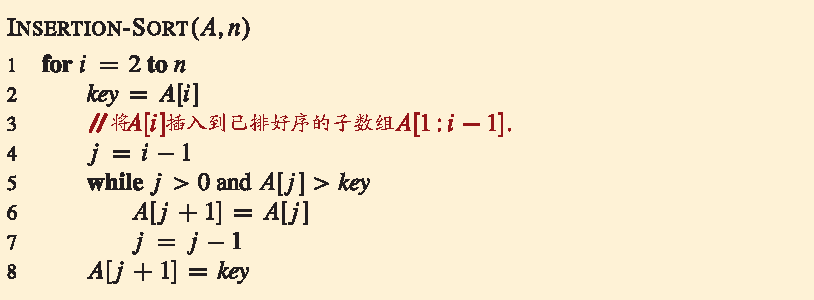
\includegraphics{算法导论第四版插图/第二章/插入排序伪代码.pdf}

我们能观察到伪代码的操作是什么?该过程有嵌套循环。外部循环是一个\textbf{for}循环,无论排序的值如何,它都会运行$n-1$次。内部循环是一个\textbf{while}循环,但它的迭代次数取决于被排序的值。循环变量$j$从$i-1$开始,在每次迭代中递减1,直到它达到0或$A[j]\leq key$。对于给定的$i$值,\textbf{while}循环可能迭代0次,$i-1$次或任何在它们之间。\textbf{while}循环的主体(第6-7行)每次迭代都需要常数时间。

这些观察足以推导出INSERTION-SORT的任何情况的$O(n^2)$运行时间,给我们一个适用于所有输入的总体陈述。运行时间由内部循环主导。因为外部循环的$n-1$次迭代中的每一次都会导致内部循环最多迭代$i-1$次,并且因为$i$最多为$n$,内部循环的总迭代次数最多为$(n-1)(n-1)$,小于$n^2$。由于内部循环的每次迭代都需要常数时间,内部循环中花费的总时间最多是常数乘以$n^2$,即$O(n^2)$。

通过一点创造力,我们还可以看到INSERTION-SORT的最坏情况运行时间是$\Omega(n^2)$。通过说一个算法的最坏情况运行时间是$\Omega(n^2)$,我们的意思是对于每个大于某个阈值的输入大小$n$,都存在大小为$n$的至少一个输入,使得该算法需要至少$cn^2$时间,其中$c$是某个正常数。这并不一定意味着算法对于所有输入都需要至少$cn^2$时间。

\begin{figure}[htbp]
    \centering
    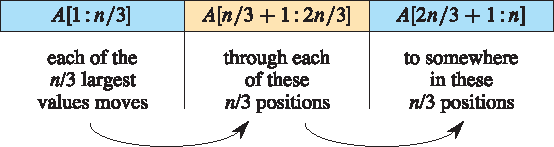
\includegraphics{算法导论第四版插图/第二章/插入排序的平均情况分析示意图.pdf}
    \caption{插入排序的$\Omega(n^2)$下界。如果前$n/3$个位置包含$n/3$个最大值,那么每个这些值都必须逐个通过中间的$n/3$个位置,一次移动一个位置,才能最终到达最后的$n/3$个位置中的某个位置。由于$n/3$个值中的每个值都至少移动了$n/3$个位置,因此在这种情况下所需的时间至少与$(n/3)(n/3)=n^2/9$成比例,即$\Omega(n^2)$。}
    \label{fig:插入排序的平均情况分析示意图}
\end{figure}

现在让我们看看为什么INSERTION-SORT的最坏情况运行时间是$\Omega(n^2)$。对于一个值要移到它起始位置的右侧,它必须在第6行中被移动。实际上,对于一个值要移动到它起始位置的右侧$k$个位置,第6行必须执行$k$次。如图\ref{fig:插入排序的平均情况分析示意图}所示,让我们假设$n$是3的倍数,这样我们就可以将数组$A$分成$n/3$个位置的组。假设在INSERTION-SORT的输入中,$n/3$个最大值占据了前$n/3$个数组位置$A[1:n/3]$。(它们在前$n/3$个位置内的相对顺序并不重要。)一旦数组被排序,这$n/3$个值中的每一个都会在最后$n/3$个位置$A[2n/3+1:n]$中的某个位置结束。为了实现这一点,这$n/3$个值中的每一个都必须通过中间的$n/3$个位置$A[n/3+1:2n/3]$。这$n/3$个值中的每一个都会逐个通过这些中间的$n/3$个位置,至少需要通过第6行$n/3$次。因为至少有$n/3$个值必须通过至少$n/3$个位置,所以INSERTION-SORT在最坏情况下所需的时间至少与$(n/3)(n/3)=n^2/9$成正比,即$\Omega(n^2)$。

因为我们已经证明了INSERTION-SORT在所有情况下都以$O(n^2)$时间运行,并且存在一种输入使其需要$\Omega(n^2)$时间,因此我们可以得出结论,INSERTION-SORT的最坏情况运行时间是$\Theta(n^2)$。上下界的常数因子可能不同并不重要。重要的是我们已经在常数因子(不计低阶项)范围内表征了最坏情况的运行时间。这个论点并没有表明INSERTION-SORT在所有情况下都以$\Theta(n^2)$时间运行。实际上,我们在第\ref{chapter-02}章中看到,最好情况的运行时间是$\Theta(n)$。

\section{渐近表示法:形式化定义}\label{section-3.2}

在非正式地了解渐近表示法后,让我们更加正式。我们用来描述算法渐近运行时间的符号是基于函数定义的,这些函数的定义域通常是自然数集合$\mathbb{N}$或实数集合$\mathbb{R}$。这些符号方便描述运行时间函数$T(n)$。本节定义了基本的渐近表示法,并介绍了一些常见的``适当''的符号滥用。

\begin{figure}
    \centering
    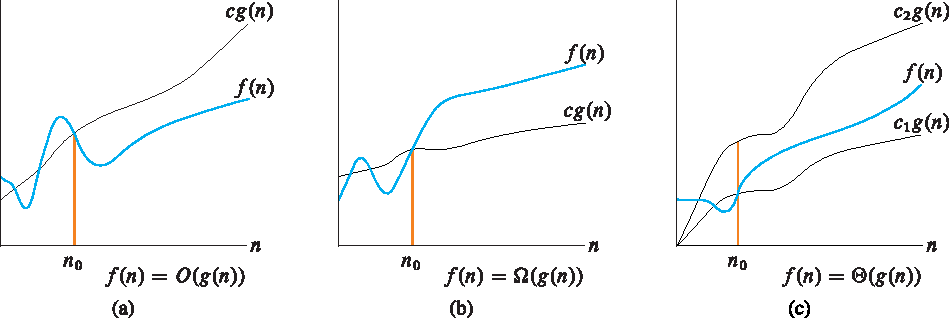
\includegraphics{算法导论第四版插图/第二章/渐近时间复杂度比较示意图.pdf}
    \caption{图是$O, \Omega$和$\Theta$符号的图形示例。在每个部分中,显示的$n_0$值是最小可能值,但任何更大的值也可以。 (a) $O$符号给出函数的上界,精确到一个常数因子。如果存在正常数$n_0$和$c$使得在$n_0$及其右侧,$f(n)$的值总是在或低于$cg(n)$上,则我们写作$f(n)=O(g(n))$。 (b) $\Omega$符号给出函数的下界,精确到一个常数因子。如果存在正常数$n_0$和$c$使得在$n_0$及其右侧,$f(n)$的值总是在或高于$cg(n)$上,则我们写作$f(n)=\Omega(g(n))$。 (c) $\Theta$符号将函数约束在常数因子之内。如果存在正常数$n_0,c_1$和$c_2$使得在$n_0$及其右侧,$f(n)$的值总是在$c_1g(n)$和$c_2g(n)$之间,则我们写作$f(n)=\Theta(g(n))$。}
    \label{fig:渐近时间复杂度比较示意图}
\end{figure}

\textbf{大$O$表示法}

正如我们在第\ref{section-3.1}节中所看到的,$O$符号描述了一个渐近上界。我们使用$O$符号给出一个函数的上界,精确到一个常数因子。

以下是$O$表示法的形式化定义。对于给定的函数$g(n)$,我们用$O(g(n))$表示函数集合

$O(g(n))=\{f(n)$ : 存在正常数$c$和$n_0$,使得
$$
\text { 对于所有的 }\; n \geq n_0 \text { 有 } \;
0 \leq f(n) \leq c g(n) \}
$$

如果存在正常数$c$使得$f(n) \leq c g(n)$对于足够大的$n$成立,则函数$f(n)$属于集合$O(g(n))$。图\ref{fig:渐近时间复杂度比较示意图}(a)展示了$O$符号的直观理解。对于所有大于等于$n_0$的$n$值,函数$f(n)$的值都在或低于$cg(n)$上。

$O(g(n))$的定义要求集合中的每个函数$f(n)$都是渐近非负的:只要$n$足够大,$f(n)$必须是非负的。(渐近正函数是指对于所有足够大的$n$,函数都是正的。)因此,函数$g(n)$本身必须是渐近非负的,否则集合$O(g(n))$为空。因此,我们假设在$O$符号中使用的每个函数都是渐近非负的。这个假设也适用于本章中定义的其他渐近表示法。

你可能会惊讶我们是如何用集合来定义$O$符号的。实际上,你可能会期望我们会写``$f(n) \in O(g(n))$'',以表示$f(n)$属于集合$O(g(n))$。相反,我们通常写``$f(n)=O(g(n))$'',并说``$f(n)$是$g(n)$的大$O$'',以表达相同的概念。虽然一开始可能会感到混乱,但在本节后面我们将看到这样做的好处。

让我们探讨一个例子,说明如何使用$O$符号的正式定义来证明我们丢弃低阶项和忽略最高阶项的常数系数的做法是正确的。我们将展示$4 n^2+100 n+500=O(n^2)$,即使低阶项的系数比主项大得多。我们需要找到正常数$c$和$n_0$,使得对于所有$n \geq n_0$,都有$4 n^2+100 n+500 \leq c n^2$。将两边都除以$n^2$得到$4+100 / n+500 / n^2 \leq c$。这个不等式对于许多$c$和$n_0$的选择都成立。例如,如果我们选择$n_0=1$,那么这个不等式对于$c=604$成立。如果我们选择$n_0=10$,那么$c=19$可以工作,选择$n_0=100$允许我们使用$c=5.05$。

我们也可以使用$O$符号的正式定义来证明函数$n^3-100 n^2$不属于集合$O(n^2)$,即使$n^2$的系数是一个大的负数。如果我们有$n^3-100 n^2=O(n^2)$,那么就会有正常数$c$和$n_0$,使得对于所有$n \geq n_0$,都有$n^3-100 n^2 \leq c n^2$。同样,我们将两边都除以$n^2$,得到$n-100 \leq c$。无论我们为常数$c$选择什么值,这个不等式都不成立,对于任何$n>c+100$的值都不成立。

\textbf{大$\Omega$表示法}

正如$O$符号提供了一个函数的渐近上界,$\Omega$符号提供了一个渐近下界。对于给定的函数$g(n)$,我们用$\Omega(g(n))$表示函数集合:

$\Omega(g(n))=\{f(n)$:存在正常数$c$和$n_0$,使得对于所有$n \geq n_0$,都有$0 \leq c g(n) \leq f(n)\}$。

图\ref{fig:渐近时间复杂度比较示意图}(b)展示了$\Omega$符号的直观理解。对于所有$n$值,包括或在$n_0$右侧的值,$f(n)$的值在或以上$c g(n)$。

我们已经展示了$4n^2+100n+500=O(n^2)$。现在让我们展示$4n^2+100n+500=\Omega(n^2)$。我们需要找到正常数$c$和$n_0$,使得对于所有$n \geq n_0$,都有$4 n^2+100 n+500 \geq c n^2$。与之前一样,我们将两边都除以$n^2$,得到$4+100 / n+500 / n^2 \geq c$。当$n_0$为任何正整数且$c=4$时,这个不等式成立。

如果我们从$4n^2$项中减去低阶项而不是加上它们会怎么样?如果$n^2$项的系数很小怎么办?函数仍然是$\Omega(n^2)$。例如,让我们展示$n^2 / 100-100 n-500=\Omega(n^2)$。除以$n^2$得到$1 / 100-100 / n-500 / n^2 \geq c$。我们可以选择任何大于或等于10,005的$n_0$值,并找到一个正值$c$。例如,当$n_0=10,005$时,我们可以选择$c=2.49 \times 10^{-9}$。是的,那是一个非常小的$c$值,但它是正数。如果我们选择更大的$n_0$值,我们也可以增加$c$值。例如,如果$n_0=100,000$,那么我们可以选择$c=0.0089$。$n_0$值越高,我们就越可以选择接近系数$1 / 100$的$c$值。

\textbf{大$\Theta$表示法}

我们使用$\Theta$符号表示渐近紧密界限。对于给定的函数$g(n)$,我们用$\Theta(g(n))$表示函数集合:

$\Theta(g(n))=\{f(n)$:存在正常数$c_1, c_2$和$n_0$,使得对于所有$n \geq n_0$,都有$0 \leq c_1 g(n) \leq f(n) \leq c_2 g(n)\}$。

图\ref{fig:渐近时间复杂度比较示意图}(c)展示了$\Theta$符号的直观理解。对于所有$n$值,包括或在$n_0$右侧的值,$f(n)$的值在或以上$c_1 g(n)$并在或以下$c_2 g(n)$。换句话说,对于所有$n \geq n_0$,函数$f(n)$与常数因子内的$g(n)$相等。

$O, \Omega$和$\Theta$表示法的定义可以推出以下定理

\begin{theorem}{}{定理3.1}
对于任何两个函数$f(n)$和$g(n)$,当且仅当$f(n)=O(g(n))$且$f(n)=\Omega(g(n))$时,我们有$f(n)=\Theta(g(n))$。
\end{theorem}

我们一般将定理\ref{thm:定理3.1}用在证明渐近紧界上面,也就是用渐近上界和渐近下界来证明渐近紧界。

\textbf{渐近表示法和运行时间}

当使用渐近表示法来描述算法的运行时间时,确保所使用的渐近表示法尽可能精确,而不会过度陈述其适用于哪个运行时间。以下是一些使用渐近表示法来描述运行时间的正确和不正确的示例。

让我们从插入排序开始。我们可以正确地说插入排序的最坏运行时间是$O(n^2), \Omega(n^2)$,并且由于\ref{thm:定理3.1},$\Theta(n^2)$。虽然三种描述最坏情况运行时间的方式都是正确的,但$\Theta(n^2)$界限是最精确和最受欢迎的。同样地,我们可以正确地说插入排序的最佳情况运行时间为$O(n), \Omega(n)$和$\Theta(n)$,其中$\Theta(n)$最精确,因此最受欢迎。

以下说法都不完全正确:插入排序的运行时间是$\Theta(n^2)$。这是一种夸大其词的说法,因为通过省略声明中的``最坏情况'',我们留下了一个涵盖所有情况的概括性陈述。错误在于插入排序并不总是在$\Theta(n^2)$时间内运行,因为正如我们所见,它在最佳情况下运行时间为$\Theta(n)$。但我们可以正确地说插入排序的运行时间是$O(n^2)$,因为在所有情况下,它的运行时间都不会超过$n^2$。当我们使用$O(n^2)$而不是$\Theta(n^2)$时,没有问题出现,即使有些情况下运行时间增长得比$n^2$慢。同样地,我们不能正确地说插入排序的运行时间是$\Theta(n)$,但我们可以说它的运行时间是$\Omega(n)$。

归并排序呢?由于归并排序在所有情况下都以$\Theta(n\lg n)$时间运行,我们可以只说它的运行时间是$\Theta(n\lg n)$,而不指定最坏情况、最佳情况或任何其他情况。

有时人们会混淆$O$符号和$\Theta$符号,错误地使用$O$符号来表示渐近紧密界限。他们会说:“一个$O(n\lg n)$时间复杂度的算法比一个$O(n^2)$时间复杂度的算法运行得更快。”也许是这样,也许不是。由于$O$符号仅表示渐近上界,所谓的$O(n^2)$时间复杂度的算法实际上可能在$\Theta(n)$时间内运行。你应该小心选择适当的渐近表示法。如果要表示渐近紧密界限,请使用$\Theta$符号。

我们通常使用渐近表示法来提供最简单和最精确的界限。例如,如果一个算法在所有情况下的运行时间为$3n^2+20n$,我们使用渐近表示法来写出它的运行时间为$\Theta(n^2)$。严格来说,我们也可以写出运行时间为$O(n^3)$或$\Theta(3n^2+20n)$。然而,在这种情况下,这些表达式都不如写$\Theta(n^2)$有用:如果运行时间为$3n^2+20n$,那么$O(n^3)$不如$\Theta(n^2)$精确,而$\Theta(3n^2+20n)$引入了复杂性,混淆了增长的量级。通过编写最简单和最精确的界限,例如$\Theta(n^2)$,我们可以对不同的算法进行分类和比较。在整本书中,你将看到几乎所有的渐近运行时间都基于多项式和对数函数:例如$n$,$n \lg ^2 n$,$n^2 \lg n$或$n^{1 / 2}$。你还将看到其他一些函数,例如指数,$\lg \lg n$和$\lg ^* n$(请参见第\ref{section-3.3}节)。通常很容易比较这些函数的增长速度。

\textbf{等式和不等式中的渐近表示法}

虽然我们正式地将渐近表示法定义为集合,但在公式中,我们使用等号$(=)$而不是集合成员符号$(\in)$。例如,我们写道$4n^2+100n+500=O(n^2)$。我们还可以写成$2n^2+3n+1=2n^2+\Theta(n)$。我们如何解释这样的公式?

当渐近表示法单独出现在等式(或不等式)的右侧时,例如$4n^2+100n+500=O(n^2)$,等号表示集合成员关系:$4n^2+100n+500 \in O(n^2)$。然而,通常情况下,当渐近表示法出现在公式中时,我们将其解释为代表某个我们不想命名的匿名函数。例如,公式$2n^2+3n+1=2n^2+\Theta(n)$表示$2n^2+3n+1=2n^2+f(n)$,其中$f(n) \in \Theta(n)$。在这种情况下,我们让$f(n)=3n+1$,它确实属于$\Theta(n)$。

以这种方式使用渐近表示法可以帮助消除方程中不必要的细节和杂乱。例如,在第\ref{chapter-02}章中,我们将归并排序的最坏运行时间表示为递归式

$$
T(n)=2T(n/2)+\Theta(n)
$$

如果我们只关心$T(n)$的渐近行为,那么没有必要准确指定所有低阶项,因为它们都被理解为包含在由术语$\Theta(n)$表示的匿名函数中。

这段文字讲解了渐近表示法在表达式中的应用。其中,匿名函数的数量被理解为渐近表示法出现的次数。例如,在表达式$$\sum_{i=1}^n O(i)$$中,只有一个匿名函数(一个关于$i$的函数)。因此,这个表达式与$O(1)+O(2)+\cdots+O(n)$不同,后者没有一个清晰的解释。

在某些情况下,渐近表示法出现在等式的左侧,如$$2 n^2+\Theta(n)=\Theta(n^2)$$使用以下规则解释这样的等式:无论在等号左边如何选择匿名函数,总有一种方式可以选择等号右边的匿名函数使等式成立。因此,我们的例子意味着对于任何$\Theta(n)$中的函数$f(n)$,都存在一些$\Theta(n^2)$中的函数$g(n)$,使得$2 n^2+f(n)=g(n)$对于所有的$n$都成立。换句话说,等式的右侧提供了比左侧更粗略的细节。

这段文字讲解了如何将多个等式链在一起。例如,我们可以将以下关系组合在一起:

$$
\begin{aligned}
2 n^2+3 n+1 & =2 n^2+\Theta(n) \\
& =\Theta(n^2)
\end{aligned}
$$

按照上述规则,分别解释每个等式。第一个等式表示存在一些函数$f(n) \in \Theta(n)$,使得对于所有的$n$,$2 n^2+3 n+1=2 n^2+f(n)$。第二个等式表示对于任何函数$g(n) \in \Theta(n)$(例如刚才提到的$f(n)$),都存在一些函数$h(n) \in \Theta(n^2)$,使得对于所有的$n$,$2 n^2+g(n)=h(n)$。这种解释意味着$2 n^2+3 n+1=\Theta(n^2)$,这正是等式链的直观含义。

\textbf{渐近表示法的适当的滥用}

这段文字讲解了渐近表示法的滥用问题。除了将等号滥用为集合成员关系,我们现在可以看到它具有精确的数学解释,还有一种滥用渐近表示法的情况,即必须从上下文中推断趋向于$\infty$的变量。例如,当我们说$O(g(n))$时,我们可以假设我们关注$g(n)$随着$n$的增长而增长,如果我们说$O(g(m))$,我们就是在谈论$g(m)$随着$m$的增长而增长。表达式中的自由变量指示了哪个变量趋向于$\infty$。

需要上下文知识来确定哪个变量趋向于$\infty$的最常见情况是,当渐近表示法内部的函数是常数时,例如表达式$O(1)$。我们无法从表达式中推断出哪个变量趋向于$\infty$,因为表达式中没有变量。上下文必须消除歧义。例如,如果使用渐近表示法的等式是$f(n)=O(1)$,那么很明显我们感兴趣的变量是$n$。然而,从上下文中知道感兴趣的变量是$n$,可以通过使用$O$符号的正式定义来理解这个表达式:表达式$f(n)=O(1)$意味着随着$n$趋近于$\infty$,函数$f(n)$的上界是常数。从技术上讲,如果我们在渐近表示法本身中明确指示趋向于$\infty$的变量可能会更少歧义,但那会使符号变得混乱。相反,我们只需确保上下文清楚地表明哪个变量(或变量)趋向于$\infty$即可。

当渐近表示法内部的函数被正常数限制时,例如$T(n)=O(1)$,我们通常会以另一种方式滥用渐近表示法,尤其是在陈述递归关系式时。我们可能会写出类似于$T(n)=O(1)$,其中$n<3$。根据$O$符号的正式定义,这个陈述是没有意义的,因为定义只说明对于某个$n_0>0$,当$n \geq n_0$时,$T(n)$的上界是正的常数$c$。$n<n_0$时,$T(n)$的值不一定受到限制。因此,在例子$T(n)=O(1)$中,当$n<3$时,我们不能推断出任何关于$T(n)$的限制,因为可能$n_0>3$。

当我们说$T(n)=O(1)$,其中$n<3$时,通常意味着存在一个正的常数$c$,使得$n<3$时$T(n) \leq c$。这种惯例使我们省去了命名限制常数的麻烦,使其保持匿名状态,同时我们将注意力集中在分析中更重要的变量上。其他渐近表示法也有类似的滥用。例如,$T(n)=\Theta(1)$,其中$n<3$表示当$n<3$时,$T(n)$在正数常数上下限制。

偶尔,描述算法运行时间的函数可能无法定义某些输入大小,例如,当算法假设输入大小是2的精确幂时。我们仍然使用渐近表示法来描述运行时间的增长,理解任何限制仅适用于函数被定义的情况。例如,假设$f(n)$仅在自然数或非负实数的子集上定义。那么,$f(n)=O(g(n))$意味着在$f(n)$的定义域上,即在$f(n)$被定义的地方,对于所有$n \geq n_0$,$O$符号定义中的界$0 \leq T(n) \leq c g(n)$成立。这种滥用很少被指出,因为通常从上下文中可以清楚地理解其含义。

在数学中,滥用符号是可以接受的,而且经常是可取的,只要我们不误用它。如果我们清楚地理解了滥用的含义,并且不得出错误的结论,它可以简化我们的数学语言,有助于提高我们的高层次理解,并帮助我们专注于真正重要的事情。

\textbf{小$o$表示法}

$O$表示法提供的渐近上界可能是渐近紧的,也可能不是。界$2 n^2=O(n^2)$是渐近紧的,但界$2 n=O(n^2)$不是。我们使用小$o$符号来表示不是渐近紧的上界。我们正式定义小$o(g(n))$为集合

$$
o(g(n))=\{f(n):\text { 对于任何正常数} c>0,\text{存在常数} n_0>0 \text {,使得} 0 \leq f(n)<c g(n) \text {对于所有} n \geq n_0\}。
$$

例如,$2 n=O(n^2)$,但$2 n^2 \neq O(n^2)$。

$O$符号和小$o$符号的定义相似。主要区别在于,在$f(n)=O(g(n))$中,界$0 \leq f(n) \leq c g(n)$对于某些正常数$c>0$成立,但在$f(n)=o(g(n))$中,界$0 \leq f(n)<c g(n)$对于所有正常数$c>0$成立。直观地说,在小$o$符号中,当$n$变大时,函数$f(n)$相对于$g(n)$变得微不足道:

$$
\lim _{n \rightarrow \infty} \frac{f(n)}{g(n)}=0
$$

一些作者使用这个极限作为小$o$表示法的定义,但本书中的定义也限制了匿名函数为渐近非负。

\textbf{$\omega$记号}

类比于$O$符号和$o$符号,$\omega$符号是$\Omega$符号的对应物。我们使用$\omega$符号来表示不是渐近紧的下界。一种定义方法是:

当且仅当$g(n) \in o(f(n))$时,$f(n) \in \omega(g(n))$。

然而,正式地,我们将$\omega(g(n))$(``$g$的$n$的小$\omega$'')定义为集合

$$
\omega(g(n))=\{f(n):\text { 对于任何正常数} c>0,\text{存在常数} n_0>0 \text {,使得}\text {对于所有} n \geq n_0 \text{有} 0 \leq c g(n)<f(n) \}。
$$

在$o$符号的定义中,$f(n)<c g(n)$,而在$\omega$符号的定义中,则相反:

$\operatorname{cg}(n)<f(n)$。对于$\omega$符号的例子,我们有$n^2 / 2=\omega(n)$,但$n^2 / 2 \neq \omega(n^2)$。关系$f(n)=\omega(g(n))$意味着
$$
\lim _{n \rightarrow \infty} \frac{f(n)}{g(n)}=\infty
$$

如果极限存在。也就是说,当$n$变大时,$f(n)$相对于$g(n)$变得任意大。

\textbf{比较函数}

许多实数的关系属性也适用于渐近比较。对于以下内容,请假设$f(n)$和$g(n)$是渐近正的。

\textbf{传递性}

\begin{equation*}
\begin{array}{llll}
f(n)=\Theta(g(n)) \text { 且 } g(n)=\Theta(h(n)) & \text { 可得 } & f(n)=\Theta(h(n)), \\
f(n)=O(g(n)) \text { 且 } g(n)=O(h(n)) & \text { 可得 } & f(n)=O(h(n)), \\
f(n)=\Omega(g(n)) \text { 且 } g(n)=\Omega(h(n)) & \text { 可得 } & f(n)=\Omega(h(n)), \\
f(n)=o(g(n)) \text { 且 } g(n)=o(h(n)) & \text { 可得 } & f(n)=o(h(n)), \\
f(n)=\omega(g(n)) \text { 且 } g(n)=\omega(h(n)) & \text { 可得 } & f(n)=\omega(h(n)) .
\end{array}
\end{equation*}

\textbf{反身性}

\begin{equation*}
\begin{aligned}
& f(n)=\Theta(f(n)), \\
& f(n)=O(f(n)), \\
& f(n)=\Omega(f(n)) .
\end{aligned}
\end{equation*}

\textbf{对称性}

$$
f(n)=\Theta(g(n)) \text { 当且仅当 } g(n)=\Theta(f(n))
$$

\textbf{对称转换}

\begin{equation*}
\begin{array}{ll}
f(n)=O(g(n)) & \text { 当且仅当 } g(n)=\Omega(f(n)) \\
f(n)=o(g(n)) & \text { 当且仅当 } g(n)=\omega(f(n))
\end{array}
\end{equation*}

由于这些属性适用于渐近表示法,我们可以将两个函数$f$和$g$的渐近比较与两个实数$a$和$b$的比较进行类比:

$f(n)=O(g(n))$ 类似 $a \leq b$,

$f(n)=\Omega(g(n))$ 类似 $a \geq b$,

$f(n)=\Theta(g(n))$ 类似 $a=b$,

$f(n)=o(g(n))$ 类似 $a<b$,

$f(n)=\omega(g(n))$ 类似 $a>b$.

如果$f(n)=o(g(n))$,我们称$f(n)$渐近小于$g(n)$;如果$f(n)=\omega(g(n))$,我们称$f(n)$渐近大于$g(n)$。

然而,实数的一个属性不能转化为渐近表示法:

\textbf{三分律}:对于任何两个实数$a$和$b$,恰好有一个成立:$a<b, a=b$或$a>b$。

虽然可以比较任何两个实数,但并非所有函数都是渐近可比的。也就是说,对于两个函数$f(n)$和$g(n)$,可能既不满足$f(n)=O(g(n))$,也不满足$f(n)=\Omega(g(n))$。例如,我们无法使用渐近表示法比较函数$n$和$n^{1+\sin n}$,因为$n^{1+\sin n}$中的指数值在0和2之间振荡,并取得了其中的所有值。

\section{标准记号和常用函数}\label{section-3.3}

本节回顾了一些标准的数学函数和符号,并探讨了它们之间的关系。它还说明了渐近表示法的使用。

\textbf{单调性}

如果$m\leq n$意味着$f(m)\leq f(n)$,则函数$f(n)$是单调递增的。类似地,如果$m\leq n$意味着$f(m)\geq f(n)$,则它是单调递减的。如果$m<n$意味着$f(m)<f(n)$,则函数$f(n)$是严格递增的;如果$m<n$意味着$f(m)>f(n)$,则函数$f(n)$是严格递减的。

\textbf{向下取整和向上取整}

对于任何实数$x$,我们用$\lfloor x\rfloor$(读作“$x$的底部”)表示不大于$x$的最大整数,用$\lceil x\rceil$(读作“$x$的顶部”)表示不小于$x$的最小整数。向下取整函数是单调递增的,向上取整函数也是如此。

向下取整和向上取整遵循以下属性。对于任何整数$n$,我们有

\begin{equation}\label{eq:3.1}
\lfloor n\rfloor=n=\lceil n\rceil
\end{equation}

对于所有实数$x$,我们有:

\begin{equation}\label{eq:3.2}
x-1<\lfloor x\rfloor \leq x \leq\lceil x\rceil<x+1
\end{equation}

我们还有

\begin{equation}\label{eq:3.3}
-\lfloor x\rfloor=\lceil-x\rceil
\end{equation}

或者等价的,

\begin{equation}\label{eq:3.4}
-\lceil x\rceil=\lfloor-x\rfloor
\end{equation}

对于任意实数 $x \geq 0$ 和整数 $a, b>0$,我们有

\begin{equation}\label{eq:3.5}
\lceil\frac{\lceil x / a\rceil}{b}\rceil=\lceil\frac{x}{a b}\rceil
\end{equation}

\begin{equation}\label{eq:3.6}
\lfloor\frac{\lfloor x / a\rfloor}{b}\rfloor=\lfloor\frac{x}{a b}\rfloor
\end{equation}

\begin{equation}\label{eq:3.7}
\lceil\frac{a}{b}\rceil \leq \frac{a+(b-1)}{b}
\end{equation}

\begin{equation}\label{eq:3.8}
\lfloor\frac{a}{b}\rfloor \geq \frac{a-(b-1)}{b}
\end{equation}

对于任意整数 $n$ 和实数 $x$,我们有

\begin{equation}\label{eq:3.9}
\lfloor n+x\rfloor=n+\lfloor x\rfloor
\end{equation}

\begin{equation}\label{eq:3.10}
\lceil n+x\rceil=n+\lceil x\rceil
\end{equation}

\textbf{模运算}

对于任何整数$a$和任何正整数$n$,$a \bmod n$的值是商$a / n$的余数(或者说模数):

\begin{equation}\label{eq:3.11}
a \bmod n=a-n\lfloor a / n\rfloor。
\end{equation}

即使$a$是负数,也有

\begin{equation}\label{eq:3.12}
0 \leq a \bmod n<n。
\end{equation}

如果已经定义了一个整数除以另一个整数时的余数的明确概念,则提供特殊的符号来表示余数的相等是方便的。如果$(a \bmod n)=(b \bmod n)$,我们写作$a=b(\bmod n)$,并说$a$等价于$b$,模$n$。换句话说,当$a$和$b$除以$n$时余数相同时,$a=b(\bmod n)$。等价地,当且仅当$n$是$b-a$的因子时,$a=b(\bmod n)$。如果$a$与$b$在模$n$意义下不等价,则写作$a \neq b(\bmod n)$。

\textbf{多项式}

给定非负整数$d$,$n$的$d$次多项式是形如

$$
p(n)=\sum_{i=0}^d a_i n^i,
$$

的函数$p(n)$,其中常数$a_0, a_1, \ldots, a_d$是多项式的系数,且$a_d \neq 0$。当且仅当$a_d>0$时,多项式是渐近正的。对于渐近正的$d$次多项式$p(n)$,有$p(n)=\Theta(n^d)$。对于任何实常数$a \geq 0$,函数$n^a$是单调递增的,而对于任何实常数$a \leq 0$,函数$n^a$是单调递减的。如果$f(n)=O(n^k)$,则称函数$f(n)$是多项式有界的,其中$k$是某个常数。

\textbf{指数}

对于所有的实数 $a>0, m$ 和 $n$,我们有以下性质:

$$
\begin{aligned}
a^0 & =1, \\
a^1 & =a, \\
a^{-1} & =1 / a, \\
(a^m)^n & =a^{m n}, \\
(a^m)^n & =(a^n)^m \\
a^m a^n & =a^{m+n} .
\end{aligned}
$$

对于所有的 $n$ 和 $a \geq 1$,函数 $a^n$ 对于 $n$ 单调递增。某些时候,我们假定 $0^0=1$。

我们可以通过以下事实将多项式和指数函数的增长速率联系起来。对于所有实常数$a>1$和$b$,有:

$$
\lim _{n \rightarrow \infty} \frac{n^b}{a^n}=0
$$

从上面的式子我们可以得出以下结论:

\begin{equation}\label{eq:3.13}
n^b=o(a^n)
\end{equation}

因此,任何底数严格大于1的指数函数增长速度都比任何多项式函数快。

使用$e$表示自然对数函数的底数$2.71828 \ldots$,对于所有实数$x$,我们有:

$$
e^x=1+x+\frac{x^2}{2 !}+\frac{x^3}{3 !}+\cdots=\sum_{i=0}^{\infty} \frac{x^i}{i !}
$$

其中``!''表示本节后面定义的阶乘函数。对于所有实数$x$,我们有以下不等式:

\begin{equation}\label{eq:3.14}
1+x \leq e^x
\end{equation}

等号成立当且仅当$x=0$。当$|x| \leq 1$时,我们有近似关系

\begin{equation}\label{eq:3.15}
1+x \leq e^x \leq 1+x+x^2
\end{equation}

当$x \rightarrow 0$时,用$1+x$来近似$e^x$是相当好的:

$$
e^x=1+x+\Theta(x^2)
$$

(在这个方程中,渐近表示法用于描述$x \rightarrow 0$时的极限行为,而不是$x \rightarrow \infty$。)对于所有$x$,我们有:

\begin{equation}\label{eq:3.16}
\lim _{n \rightarrow \infty}(1+\frac{x}{n})^n=e^x
\end{equation}

\textbf{对数}

我们使用以下记号:

$$
\begin{aligned}
\lg n & =\log _2 n & & \text { (二分对数), } \\
\ln n & =\log _e n & & \text { (自然对数), } \\
\lg ^k n & =(\lg n)^k & & \text { (对数的指数) } \\
\lg \lg n & =\lg (\lg n) & & \text { (组合). }
\end{aligned}
$$

我们采用以下符号约定:在没有括号的情况下,$\lg n+1$表示$(\lg n)+1$而不是$\lg (n+1)$。

对于任何常数$b>1$,如果$n \leq 0$,则函数$\log _b n$未定义,如果$n>0$,则函数严格单调递增,如果$0<n<1$,则函数为负,如果$n>1$,则函数为正,如果$n=1$,则函数为0。对于所有实数$a>0, b>0, c>0$和$n$,我们有:

\begin{equation}\label{eq:3.17}
a=b^{\log _b a}
\end{equation}

\begin{equation}\label{eq:3.18}
\log _c(a b)=\log _c a+\log _c b
\end{equation}

\begin{equation}\label{eq:3.19}
\begin{aligned}
\log _b a^n&=n \log _b a, \\
\log _b a&=\frac{\log _c a}{\log _c b}
\end{aligned}
\end{equation}

\begin{equation}\label{eq:3.20}
\log _b(1 / a)=-\log _b a,
\end{equation}

\begin{equation}\label{eq:3.21}
\begin{aligned}
\log _b a &= \frac{1}{\log _a b} \\
a^{\log _b c} &= c^{\log _b a}
\end{aligned}
\end{equation}

这里,上面的每个等式中,对数的底都是1。

根据等式\eqref{eq:3.19},将对数的底从一个常数变为另一个常数只会使对数的值乘以一个常数因子。因此,我们经常在不关心常数因子的情况下使用符号“$\lg n$”,例如在$O$符号中。计算机科学家发现2是对数最自然的底数,因为许多算法和数据结构涉及将问题分成两部分。当$|x|<1$时,$\ln (1+x)$有一个简单的级数展开式:

\begin{equation}\label{eq:3.22}
\ln (1+x)=x-\frac{x^2}{2}+\frac{x^3}{3}-\frac{x^4}{4}+\frac{x^5}{5}-\cdots
\end{equation}

对于 $x>-1$,我们同样有以下不等式:

\begin{equation}\label{eq:3.23}
\frac{x}{1+x} \leq \ln (1+x) \leq x
\end{equation}

等号仅在$x=0$时成立。

如果$f(n)=O(\lg^kn)$,其中$k$是某个常数,则称函数$f(n)$是\textbf{多对数有界}的。我们可以通过在等式\eqref{eq:3.13}中将$n$替换为$\lg n$,将$a$替换为$2^a$,来将多项式和多对数的增长联系起来。对于所有实常数$a>0$和$b$,我们有:

\begin{equation}\label{eq:3.24}
\lg ^b n=o(n^a)
\end{equation}

因此,任何正的多项式函数的增长速度都比任何多对数函数快。

\textbf{阶乘}

记号 $n!$(读作``$n$的阶乘'')定义为当整数 $n \geq 0$ 时,

$$
n != \begin{cases}1 & \text { 如果 } n=0 \\ n \cdot(n-1) ! & \text { 如果 } n>0 .\end{cases}
$$

从而有,$n !=1 \cdot 2 \cdot 3 \cdots n$.

阶乘函数有一个相对宽松的上界:$n ! \leq n^n$,因为$n$的阶乘中的每一项最大也就是 $n$。下面是阶乘的Stirling近似:

\begin{equation}
n !=\sqrt{2 \pi n}(\frac{n}{e})^n(1+\Theta(\frac{1}{n})),
\end{equation}

$e$ 是自然对数的底,Stirling近似给了我们一个阶乘函数的更加严格的上界和更加严格的下界。

\begin{equation}
n!=o(n^n)
\end{equation}

\begin{equation}
n!=\omega(2^n)
\end{equation}

\begin{equation}
\lg(n!)=\Theta(n\lg n),
\end{equation}

Stirling近似在证明等式(3.28)时很有用。下面的等式对于所有的 $n \geq 1$ 都成立:

\begin{equation}
n !=\sqrt{2 \pi n}(\frac{n}{e})^n e^{\alpha_n}
\end{equation}

这里

$$
\frac{1}{12 n+1}<\alpha_n<\frac{1}{12 n}
$$

\textbf{迭代函数}

我们使用符号$f^{(i)}(n)$表示函数$f(n)$迭代应用$i$次到$n$的初始值。形式上,假设$f(n)$是实数上的一个函数。对于非负整数$i$,我们递归地定义:

\begin{equation}
f^{(i)}(n)= \begin{cases}n & \text { 如果 } i=0 \\ f(f^{(i-1)}(n)) & \text { 如果 } i>0\end{cases}
\end{equation}

例如,如果有 $f(n)=2 n$,那么 $f^{(i)}(n)=2^i n$ 。

\textbf{迭代对数函数}

我们使用符号$\lg ^* n$表示迭代对数,定义如下。让$\lg ^{(i)} n$如上所述,其中$f(n)=\lg n$。因为非正数的对数是未定义的,所以只有在$\lg ^{(i-1)} n>0$时,$\lg ^{(i)} n$才有定义。请注意将$\lg ^{(i)} n$(连续应用$i$次的对数函数,以$n$为参数开始)与$\lg ^i n$(将$n$取对数$i$次)区分开来。然后我们定义迭代对数函数为:

$$
\lg ^* n=\min \{i \geq 0: \lg ^{(i)} n \leq 1\}
$$

迭代对数是一个增长非常非常慢的函数:

$$
\begin{aligned}
\operatorname{gg}^* 2 & =1 \\
\mathrm{gg}^* 4 & =2 \\
\lg ^* 16 & =3, \\
\lg ^* 65536 & =4 \\
\lg ^*(2^{65536}) & =5
\end{aligned}
$$

由于可观察宇宙中的原子数量估计约为$10^{80}$,远小于$2^{65536}=10^{65536 / \lg 10} \approx 10^{19,728}$,因此我们很少遇到一个输入大小$n$,使得$\lg ^* n>5$。

\textbf{斐波那契数}

我们将斐波那契数定义为 $F_i$,对于 $i \geq 0$,有如下成立:

\begin{equation}
F_i= \begin{cases}0 & \text { 如果 } i=0, \\ 1 & \text { 如果 } i=1 \\ F_{i-1}+F_{i-2} & \text { 如果 } i \geq 2 .\end{cases}
\end{equation}

因此,在前两个数字后,每个斐波那契数都是前两个数的和,形成了以下序列:

$$
0,1,1,2,3,5,8,13,21,34,55,\ldots
$$

斐波那契数与黄金比$\phi$及其共轭$\hat{\phi}$有关,它们是方程的两个根:

$$
x^2=x+1
$$

黄金分割率的定义如下:

\begin{equation}
\begin{aligned}
\phi & =\frac{1+\sqrt{5}}{2} \\
& =1.61803 \ldots
\end{aligned}
\end{equation}

它的共轭是

\begin{equation}
\begin{aligned}
\widehat{\phi} & =\frac{1-\sqrt{5}}{2} \\
& =-.61803 \ldots
\end{aligned}
\end{equation}

特别的,我们有公式

$$
F_i=\frac{\phi^i-\widehat{\phi}^i}{\sqrt{5}}
$$

因为 $|\hat{\phi}|<1$,所以

$$
\begin{aligned}
\frac{|\hat{\phi}^i|}{\sqrt{5}} & <\frac{1}{\sqrt{5}} \\
& <\frac{1}{2}
\end{aligned}
$$

可以推导出

\begin{equation}
F_i=\lfloor\frac{\phi^i}{\sqrt{5}}+\frac{1}{2}\rfloor
\end{equation}

也就是说,第$i$个斐波那契数$F_i$等于$\phi^i / \sqrt{5}$四舍五入到最近的整数。因此,斐波那契数呈指数增长。

\chapter{分治策略}\label{chapter-04}

分治法是设计渐近有效算法的强大策略。我们在第\ref{subsection-2.3.1}节中学习归并排序时看到了分治法的一个例子。在本章中,我们将探讨分治法的应用,并获得有价值的数学工具,可以用来解决分析分治算法时出现的递归关系式。

回想一下,对于分治法,你需要递归地解决给定问题(实例)。如果问题足够小——基本情况——你只需直接解决它而不进行递归。否则——递归情况——你需要执行三个特征步骤:

\begin{enumerate}
\item 将问题分成一个或多个子问题,这些子问题是相同问题的较小实例。
\item 通过递归地解决它们来征服子问题。
\item 将子问题的解组合成原始问题的解。
\end{enumerate}

分治算法将一个大问题分解成更小的子问题,这些子问题本身可能会被分解成更小的子问题,以此类推。当递归到达基本情况且子问题足够小以直接解决而无需进一步递归时,递归停止。

\textbf{递归式}

为了分析递归分治算法,我们需要一些数学工具。递归式是一种方程,它描述了一个函数与其在其他通常更小的参数上的值之间的关系。递归式与分治方法密不可分,因为它们为我们提供了一种用数学方式描述递归算法运行时间的自然方法。在第\ref{subsection-2.3.2}节中,我们分析归并排序的最坏情况运行时间时,看到了递归式的一个例子。

对于第\ref{section-4.1}节和第\ref{section-4.2}节中介绍的分治矩阵乘法算法,我们将推导出描述它们最坏情况运行时间的递归式。为了理解这两个分治算法为什么表现出特定的性能,你需要学习如何解决描述它们运行时间的递归式。第\ref{section-4.3}--\ref{section-4.7}节介绍了几种解决递归式的方法。这些部分还探讨了递归式背后的数学,这可以为设计自己的分治算法提供更强的直觉。

我们希望尽快了解算法。因此,让我们现在只介绍一些递归式基础知识,然后在看完矩阵乘法示例后,我们将更深入地研究递归式,特别是如何解决它们。

递归式的一般形式是一个方程或不等式,使用函数本身描述整数或实数上的一个函数。它包含两个或多个情况,具体取决于参数。如果一个情况涉及在不同(通常更小)的输入上递归调用函数,则它是一个递归情况。如果一个情况不涉及递归调用,则它是一个基本情况。可能有0个、1个或多个函数满足递归式的声明。如果至少有一个函数满足它,则递归式是明确定义的,否则是不明确定义的。

\textbf{算法递归式}

我们将特别关注描述分治算法运行时间的递归式。如果对于每个充分大的阈值常数$n_0>0$,递归式$T(n)$满足以下两个性质,则它是算法递归式:

\begin{enumerate}
\item 对于所有$n<n_0$,我们有$T(n)=\Theta(1)$。
\item 对于所有$n \geq n_0$,每个递归调用路径都在有限数量的递归调用内终止于定义的基本情况。
\end{enumerate}

类似于我们有时滥用渐近表示法,当一个函数未定义于所有参数时,我们理解这个定义受限于$T(n)$被定义的$n$值。

为什么表示(正确的)分治算法最坏情况运行时间的递归式$T(n)$会满足所有充分大的阈值常数的这些性质呢?第一个性质表明存在常数$c_1, c_2$,使得对于$n<n_0$,有$0<c_1 \leq T(n) \leq c_2$。对于每个合法输入,算法必须在有限时间内输出所解决问题的解(参见第\ref{section-1.1}节)。因此,我们可以让$c_1$是调用过程并返回所需的最小时间,它必须是正的,因为需要执行机器指令来调用过程。如果某些$n$值没有合法输入,则该算法的运行时间可能对某些$n$值未定义,但它必须至少为一个$n$值定义,否则该“算法”将无法解决任何问题。因此,我们可以让$c_2$是该算法在任何大小为$n<n_0$的输入上的最大运行时间,其中$n_0$足够大,使得该算法解决大小小于$n_0$的至少一个问题。由于大小小于$n_0$的输入最多只有有限个,而且如果$n_0$足够大,则至少有一个输入。因此,$T(n)$满足第一个性质。如果第二个性质对于$T(n)$不成立,则该算法不正确,因为它将陷入无限递归循环或无法计算解。因此,可以推断出,正确的分治算法的最坏情况运行时间的递归式将是算法递归式。

\textbf{递归式的约定}

我们采用以下约定:

\begin{tcolorbox}
如果未明确说明基本情况,则假定递归式是算法递归式。
\end{tcolorbox}

这意味着你可以自由选择任何足够大的阈值常数$n_0$,使得$T(n)=\Theta(1)$的基本情况范围。有趣的是,当分析算法时,你可能会看到大多数算法递归式的渐近解不依赖于阈值常数的选择,只要它足够大使递归式定义良好即可。

在将定义在整数上的递归式转换为定义在实数上的递归式时,去掉任何向下取整或向上取整时,算法分治递归式的渐近解通常也不会改变。第\ref{section-4.7}节给出了一个足够的条件,可以忽略大多数分治递归式中的向下取整和向上取整。因此,我们经常在没有向下取整和向上取整的情况下陈述算法递归式。这样做通常简化了递归式的陈述以及与它们进行的任何数学运算。

有时你可能会看到不是方程而是不等式的递归式,例如$T(n) \leq 2 T(n / 2)+\Theta(n)$。因为这样的递归式仅陈述了$T(n)$的上限,所以我们使用$O$符号而不是$\Theta$符号来表示其解。同样地,如果将不等式反转为$T(n)\geq 2T(n/2)+\Theta(n)$,则由于递归式仅给出$T(n)$的下限,因此我们在其解中使用$\Omega$符号。

\textbf{分治算法和递归式}

本章通过使用递归式分析两个分治算法来说明分治方法,这两个算法用于矩阵乘法。第\ref{section-4.1}节介绍了一种简单的分治算法,通过将大小为$n$的矩阵乘法问题分成四个大小为$n/2$的子问题来递归地解决。该算法的运行时间可以由递归式表征:

$$
T(n)=8 T(n / 2)+\Theta(1),
$$

结果表明,该递归式的解为$T(n)=\Theta(n^3)$。虽然这种分治算法并不比使用三重嵌套循环的直接方法更快,但由于V. Strassen提出的渐近更快的分治算法,我们将在第\ref{section-4.2}节中探讨其原理。精彩的Strassen算法将大小为$n$的问题分成了七个大小为$n/2$的子问题,并递归地解决它们。Strassen算法的运行时间可以由递归式描述:

$$
T(n)=7 T(n / 2)+\Theta(n^2)
$$

该递归式的解为$T(n)=\Theta(n^{\lg 7})=O(n^{2.81})$。Strassen算法在渐近意义下超过了直接循环方法。

这两个分治算法都将大小为$n$的问题分成了几个大小为$n/2$的子问题。虽然在使用分治时,所有子问题的大小通常相同,但并非总是如此。有时将大小为$n$的问题划分为不同大小的子问题是有益的,此时描述运行时间的递归式反映了不规则性。例如,考虑一种分治算法,它将大小为$n$的问题分成一个大小为$n/3$的子问题和一个大小为$2n/3$的子问题,需要$\Theta(n)$的时间来划分问题并合并子问题的解。然后,该算法的运行时间可以由递归式描述:

$$
T(n)=T(n / 3)+T(2 n / 3)+\Theta(n)
$$

结果表明,该递归式的解为$T(n)=\Theta(n \lg n)$。我们甚至会在第\ref{chapter-09}章看到一种算法,通过递归地解决一个大小为$n/5$的子问题和一个大小为$7n/10$的子问题来解决一个大小为$n$的问题,对于划分和合并步骤需要$\Theta(n)$的时间。该算法的性能满足递归式:

$$
T(n)=T(n / 5)+T(7 n / 10)+\Theta(n)
$$

其解为$T(n)=\Theta(n)$。

虽然分治算法通常创建大小为原问题大小的常数分数的子问题,但并非总是如此。例如,线性搜索的递归版本仅创建一个子问题,其规模比原问题小一个元素。每个递归调用需要常数时间加上递归地解决一个元素较少的子问题所需的时间,导致递归式:

$$
T(n)=T(n-1)+\Theta(1)
$$

其解为$T(n)=\Theta(n)$。尽管如此,大多数高效的分治算法都解决了原问题大小的常数分数大小的子问题,这也是我们将重点关注的地方。

\textbf{求解递归式}

在第\ref{section-4.1}节和第\ref{section-4.2}节学习了矩阵乘法的分治算法之后,我们将探讨几种解决递归式的数学工具--即获得渐近$\Theta$、$O$或$\Omega$界限的工具。我们需要易于使用的工具,可以处理最常见的情况。但我们也需要通用工具,可以处理不太常见的情况,尽管需要更多的努力。本章提供了四种解决递归式的方法:

\begin{itemize}
\item 代入法(第\ref{section-4.3}节)中,你猜测一个界限的形式,然后使用数学归纳法证明你的猜测是正确的,并解出常数。这种方法可能是解决递归式最健壮的方法,但它也要求你做出一个好的猜测,并产生归纳证明。
\item 递归树法(第\ref{section-4.4}节)将递归式建模为一棵树,其节点代表递归不同层次上产生的代价。为了解决递归式,你需要确定每个层次上的代价并将它们相加,可能使用第\ref{section:A.2}节中用于界定求和的技巧。即使你不使用这种方法正式证明一个界限,它也可以帮助你猜测代入法中使用的界限形式。
\item 主方法(第\ref{section-4.5}节和第\ref{section-4.6}节)是最简单的方法,当适用时。它提供了形如

$$
T(n)=a T(n / b)+f(n)
$$

的递归式的界限,其中$a>0$和$b>1$是常数,$f(n)$是给定的“驱动”函数。这种递归式在算法研究中比其他任何递归式都更常见。它描述了一个创建$a$个子问题的分治算法,每个子问题的大小是原问题的$1/b$,使用$f(n)$的时间进行划分和合并步骤。要应用主方法,你需要记忆三种情况,但一旦你掌握了这些情况,就可以轻松确定许多分治算法的运行时间渐近界限。
\item Akra-Bazzi方法(第\ref{section-4.7}节)是解决分治递归式的通用方法。虽然它涉及微积分,但它可以用于攻击比主方法解决的更复杂的递归式。
\end{itemize}

\section{正方形矩阵相乘}\label{section-4.1}

我们可以使用分治方法来相乘方阵。如果你以前见过矩阵,那么你可能知道如何相乘它们。让$A=(a_{i k})$和$B=(b_{j k})$是方阵,都是$n \times n$。矩阵积$C=A \cdot B$也是一个$n \times n$的矩阵,其中对于$i, j=1,2, \ldots, n$,$C$的$(i, j)$项为

\begin{equation}
c_{i j}=\sum_{k=1}^n a_{i k} \cdot b_{k j}
\end{equation}

通常,我们假设矩阵是密集的,意味着大多数$n^2$个元素不为0,而不是稀疏的,其中大多数$n^2$个元素为0,非零元素可以比在$n \times n$数组中更紧凑地存储。

计算矩阵$C$需要计算$n^2$个矩阵元素,每个元素都是输入自$A$和$B$的$n$个成对乘积之和。MATRIX-MULTIPLY过程以直接的方式实现了这个策略,并略微推广了问题。它以三个$n \times n$矩阵$A, B$和$C$作为输入,并将矩阵积$A \cdot B$添加到$C$中,将结果存储在$C$中。因此,它计算的是$C=C+A \cdot B$,而不仅仅是$C=A \cdot B$。如果只需要乘积$A \cdot B$,则在调用该过程之前将所有$n^2$个元素的$C$初始化为0,这需要额外的$\Theta(n^2)$时间。我们将看到,矩阵乘法的成本在渐近意义下支配了这个初始化成本。

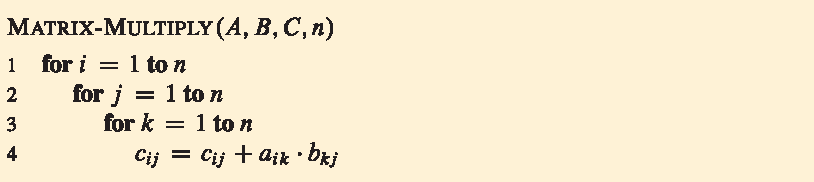
\includegraphics{算法导论第四版插图/第四章/普通矩阵相乘算法.pdf}

MATRIX-MULTIPLY的伪代码如下。第1-4行的for循环计算每一行$i$的元素,并且在给定行$i$中,第2-4行的for循环计算每个列$j$的每个元素$c_{i j}$。第3-4行的每次for循环迭代都会添加方程(4.1)的一个额外项。

因为每个三重嵌套的for循环都运行了$n$次迭代,并且每次执行第4行都需要常数时间,所以MATRIX-MULTIPLY过程的运行时间为$\Theta(n^3)$。即使我们加上将$C$初始化为0的$\Theta(n^2)$时间,运行时间仍然为$\Theta(n^3)$。

\textbf{一个简单的分治算法}

让我们看看如何使用分治方法计算矩阵积$A \cdot B$。对于$n>1$,分割步骤将$n \times n$矩阵划分为四个$n / 2 \times n / 2$子矩阵。我们假设$n$是2的幂次方,这样当算法递归时,我们可以保证子矩阵的维数是整数。与MATRIX-MULTIPLY一样,我们实际上计算的是$C=C+A \cdot B$。但是为了简化算法背后的数学,让我们假设$C$已经被初始化为零矩阵,这样我们确实在计算$C=A \cdot B$。

分解步骤将每个$n \times n$矩阵$A, B$和$C$视为四个$n / 2 \times n / 2$子矩阵:

\begin{equation}
A=(\begin{array}{ll}
A_{11} & A_{12} \\
A_{21} & A_{22}
\end{array}), \quad B=(\begin{array}{ll}
B_{11} & B_{12} \\
B_{21} & B_{22}
\end{array}), \quad C=(\begin{array}{ll}
C_{11} & C_{12} \\
C_{21} & C_{22}
\end{array})
\end{equation}

我们可以将矩阵乘积写为如下形式

\begin{equation}
(\begin{array}{ll}
C_{11} & C_{12} \\
C_{21} & C_{22}
\end{array})=(\begin{array}{ll}
A_{11} & A_{12} \\
A_{21} & A_{22}
\end{array})(\begin{array}{ll}
B_{11} & B_{12} \\
B_{21} & B_{22}
\end{array})
\end{equation}

\begin{equation}
\quad\quad\quad\quad\quad\quad\quad\quad\quad\quad\quad\quad\quad\quad
=(\begin{array}{cc}
A_{11} \cdot B_{11}+A_{12} \cdot B_{21} & A_{11} \cdot B_{12}+A_{12} \cdot B_{22} \\
A_{21} \cdot B_{11}+A_{22} \cdot B_{21} & A_{21} \cdot B_{12}+A_{22} \cdot B_{22}
\end{array}),
\end{equation}

对应了以下等式

\begin{equation}
C_{11}=A_{11} \cdot B_{11}+A_{12} \cdot B_{21}
\end{equation}

\begin{equation}
C_{12}=A_{11} \cdot B_{12}+A_{12} \cdot B_{22}
\end{equation}

\begin{equation}
C_{21}=A_{21} \cdot B_{11}+A_{22} \cdot B_{21}
\end{equation}

\begin{equation}
C_{22}=A_{21} \cdot B_{12}+A_{22} \cdot B_{22}
\end{equation}

方程(4.5)-(4.8)涉及到八个$n / 2 \times n / 2$乘法和四个$n / 2 \times n / 2$子矩阵的加法。

当我们试图将这些方程转换为可以用伪代码描述甚至实现的算法时,有两种常见的矩阵分割实现方法。

一种策略是分配临时存储空间来保存$A$的四个子矩阵$A_{11}$、$A_{12}$、$A_{21}$和$A_{22}$,以及$B$的四个子矩阵$B_{11}$、$B_{12}$、$B_{21}$和$B_{22}$。然后将$A$和$B$中的每个元素复制到相应子矩阵的相应位置。在递归征服步骤之后,将每个$C$的四个子矩阵$C_{11}$、$C_{12}$、$C_{21}$和$C_{22}$中的元素复制到它们在$C$中的相应位置。这种方法需要$\Theta(n^2)$时间,因为复制了$3n^2$个元素。

第二种方法使用索引计算,更快且更实用。可以通过指示子矩阵位于矩阵中的位置而不触及任何矩阵元素来在矩阵内指定子矩阵。将矩阵(或递归地,子矩阵)划分仅涉及对此位置信息进行算术运算,该位置信息具有与矩阵大小无关的恒定大小。对子矩阵元素的更改会更新原始矩阵,因为它们占用相同的存储空间。
接下来,我们假设使用索引计算,并且可以在$\Theta(1)$时间内执行分割。而无论是使用复制的第一种方法还是使用索引计算的第二种方法对于矩阵乘法的总渐近运行时间都没有影响。但是对于其他分治矩阵计算,例如矩阵加法,可能会有所不同。

MATRIX-MULTIPLY-RECURSIVE过程使用方程(4.5)-(4.8)来实现平方矩阵乘法的分治策略。与MATRIX-MULTIPLY一样,过程MATRIX-MULTIPLY-RECURSIVE计算$C=C+A \cdot B$,因为如果需要,在调用过程之前可以将$C$初始化为0,以仅计算$C=A \cdot B$。

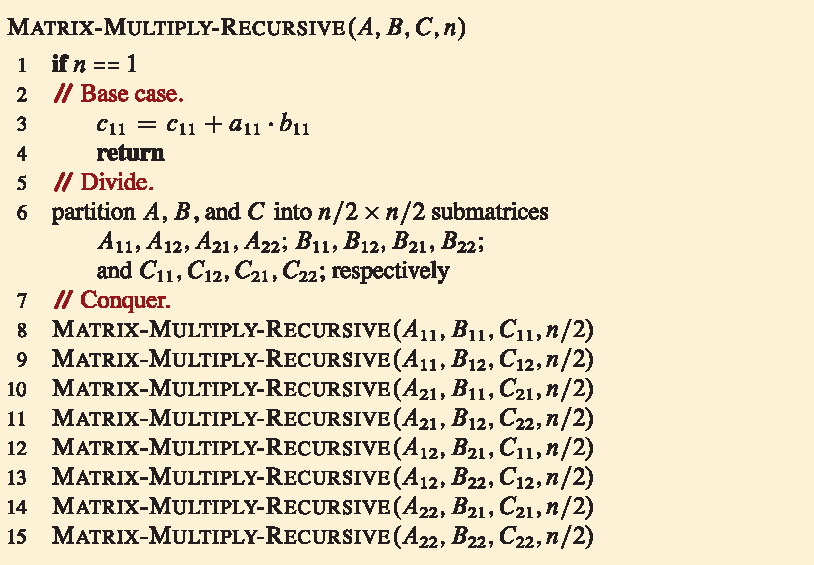
\includegraphics{算法导论第四版插图/第四章/递归矩阵相乘算法.pdf}

当我们按照伪代码进行操作时,我们将推导一个递归式来描述其运行时间。假设$T(n)$是使用此过程乘两个$n \times n$矩阵的最坏情况时间。

在基本情况下,当$n=1$时,第3行只执行一个标量乘法和一个加法,这意味着$T(1)=\Theta(1)$。按照我们的常规惯例,对于常数基本情况,我们可以在递归公式的声明中省略此基本情况。递归情况发生在$n>1$时。如前所述,我们将使用索引计算在第6行中分割矩阵,需要$\Theta(1)$的时间。第8-15行递归地调用MATRIX-MULTIPLY-RECURSIVE共八次。前4个递归调用计算方程(4.5)-(4.8)的第1项,随后的4个递归调用计算并添加第2项。每个递归调用将$A$的子矩阵和$B$的子矩阵的积添加到$C$的相应子矩阵中,得益于索引计算。因为每个递归调用乘以两个$n/2 \times n/2$矩阵,从而对总运行时间贡献了$T(n/2)$,因此所有8个递归调用所需的时间为$8 T(n/2)$。没有合并步骤,因为矩阵$C$是原地更新的。因此,递归情况的总时间是分割时间和所有递归调用的时间之和,或$\Theta(1)+8T(n/2)$。

因此,省略基本情况的声明,我们将MATRIX-MULTIPLY-RECURSIVE的运行时间递归式表示为

\begin{equation}
T(n)=8T(n/2)+\Theta(1)
\end{equation}

正如我们将在第\ref{section-4.5}节中从主方法中看到的那样,递归式(4.9)的解为$T(n)=\Theta(n^3)$,这意味着它具有与直接MATRIX-MULTIPLY过程相同的渐近运行时间。

为什么这个递归式的$\Theta(n^3)$解比归并排序递归式(2.3)的$\Theta(n\lg n)$解大得多?毕竟,归并排序的递归式包含一个$\Theta(n)$项,而递归矩阵乘法的递归式仅包含一个$\Theta(1)$项。

让我们思考一下对于递归式(4.9),递归树会与图\ref{fig:归并排序的递归树示意图}所示的归并排序递归树相比会是什么样子。归并排序递归式中的因子2决定了每个树节点有多少个子节点,进而决定了每个树层次上有多少项贡献于总和。相比之下,对于MATRIX-MULTIPLY-RECURSIVE的递归式(4.9),每个递归树内部节点有八个子节点,而不是两个,导致递归树更加``丰满'',拥有更多的叶子节点,尽管内部节点每个都要小得多。因此,递归式(4.9)的解增长速度比递归式(2.3)的解快得多,这在实际解中得到了证明:$\Theta(n^3)$与$\Theta(n \lg n)$。

\section{矩阵相乘的Strassen算法}\label{section-4.2}

你可能很难想象任何矩阵乘法算法都可以在$\Theta(n^3)$时间内完成,因为矩阵乘法的自然定义需要$n^3$个标量乘法。事实上,许多数学家认为,在1969年之前,无法在$O(n^3)$时间内计算矩阵乘积,直到Strassen发表了一种出色的递归算法,用于计算$n \times n$矩阵的乘积。Strassen的算法运行时间为$\Theta(n^{\lg 7})$。由于$\lg 7=2.8073549 \ldots$,Strassen的算法运行时间为$O(n^{2.81})$,这比$\Theta(n^3)$的MATRIX-MULTIPLY和MATRIX-MULTIPLY-RECURSIVE过程渐近更好。

Strassen方法的关键是使用MATRIX-MULTIPLY-RECURSIVE过程中的分治思想,但使递归树不那么丰满。我们实际上会通过一个常数因子增加每个分治步骤的工作量,但减少丰满性将会收益更多。我们不会将递归(4.9)的八路分支完全降至递归(2.3)的二路分支,但我们会稍微改进它,这将产生很大的差异。Strassen的算法不是执行$8$个$n / 2 \times n / 2$矩阵的递归乘法,而是只执行$7$个。消除一个矩阵乘法的代价是几个新的$n / 2 \times n / 2$矩阵的加减运算,但仍然只有一个常数。我们将采用通用术语称它们为``加法'',而不是在每个地方都说``加法和减法'',因为减法结构上与加法相同,只是符号不同。

为了了解如何减少乘法的数量,以及为什么减少乘法的数量对于矩阵计算可能是有利的,请假设你有两个数字$x$和$y$,并且你想计算量$x^2-y^2$。直接计算需要两个乘法来平方$x$和$y$,然后是一次减法(可以将其视为“负加法”)。但让我们回想一下旧的代数技巧$x^2-y^2=x^2-x y+x y-y^2=$ $x(x-y)+y(x-y)=(x+y)(x-y)$。使用所需数量的这种表述,你可以计算和$x+y$和差$x-y$,然后将它们相乘,只需要一个乘法和两个加法。以一个额外的加法为代价,只需要一个乘法来计算看起来需要两个乘法的表达式。如果$x$和$y$是标量,没有太大的区别:两种方法都需要三个标量操作。然而,如果$x$和$y$是大矩阵,那么乘法的代价将超过加法的代价,在这种情况下,第二种方法优于第一种方法,尽管不是渐近优于。

Strassen的策略是通过增加矩阵加法的代价来减少矩阵乘法的数量,这一点并不明显——也许是本书中最大的低估!与MATRIX-MULTIPLY-RECURSIVE一样,Strassen的算法使用分治方法计算$C=C+A \cdot B$,其中$A、B$和$C$均为$n \times n$矩阵,$n$是2的幂。Strassen的算法通过四个步骤从方程式(4.5)-(4.8)计算$C$的四个子矩阵$C_{11}$、$C_{12}$、$C_{21}$和$C_{22}$。我们将在分析成本的同时沿着这个过程开发一个总运行时间的递归式$T(n)$。让我们看看它是如何工作的:

\begin{enumerate}
\item 如果$n=1$,则每个矩阵只包含一个元素。执行单个标量乘法和单个标量加法,如MATRIX-MULTIPLY-RECURSIVE中的第3行,需要$\Theta(1)$时间,并返回。否则,将输入矩阵$A$和$B$以及输出矩阵$C$划分为$n/2\times n/2$子矩阵,如方程式(4.2)所示。通过索引计算,这一步需要$\Theta(1)$时间,就像MATRIX-MULTIPLY-RECURSIVE一样。
\item 创建$n/2\times n/2$矩阵$S_1$、$S_2$、$\ldots$、$S_{10}$,每个矩阵是步骤1中两个子矩阵之和或差。创建并清零七个$n/2\times n/2$矩阵$P_1、P_2、\ldots、P_7$以容纳七个$n/2\times n/2$矩阵乘积。所有17个矩阵可以在$\Theta(n^2)$时间内创建,并初始化$P_i$。
\item 使用步骤1中的子矩阵和步骤2中创建的矩阵$S_1$、$S_2$、$\ldots$、$S_{10}$,递归计算每个七个矩阵乘积$P_1$、$P_2$、$\ldots$、$P_7$,需要$7T(n/2)$时间。
\item 通过添加或减去各种$P_i$矩阵来更新结果矩阵$C$的四个子矩阵$C_{11}$、$C_{12}$、$C_{21}$、$C_{22}$,这需要$\Theta(n^2)$时间。
\end{enumerate}

我们很快就会看到步骤$2-4$的细节,但我们已经有足够的信息来建立Strassen算法运行时间的递归。通常,步骤1中的基本情况需要$\Theta(1)$时间,我们在陈述递归式时将其省略。当$n>1$时,步骤1、2和4总共需要$\Theta(n^2)$的时间,而步骤3需要对$n/2\times n/2$矩阵进行七次乘法。因此,我们得到了以下Strassen算法运行时间的递归式:

\begin{equation}
T(n)=7 T(n / 2)+\Theta(n^2)
\end{equation}

与MATRIX-MULTIPLY-RECURSIVE相比,我们为一个递归子矩阵乘法付出了一个常数数量的子矩阵加法。一旦你理解了递归和它们的解,你就能够看到这种权衡实际上导致了更低的渐近运行时间。根据第\ref{section-4.5}节中的主方法,递归式(4.10)的解为$T(n)=\Theta(n^{\lg 7})=O(n^{2.81})$,超过了$\Theta(n^3)$时间算法。

现在,让我们深入细节。第2步创建以下10个矩阵:

$$
\begin{aligned}
& S_1=B_{12}-B_{22}, \\
& S_2=A_{11}+A_{12}, \\
& S_3=A_{21}+A_{22}, \\
& S_4=B_{21}-B_{11}, \\
& S_5=A_{11}+A_{22}, \\
& S_6=B_{11}+B_{22}, \\
& S_7=A_{12}-A_{22}, \\
& S_8=B_{21}+B_{22}, \\
& S_9=A_{11}-A_{21}, \\
& S_{10}=B_{11}+B_{12} .
\end{aligned}
$$

第2步将$n/2\times n/2$矩阵相加或相减10次,需要$\Theta(n^2)$的时间。

第3步递归地乘以$n/2\times n/2$矩阵7次,计算以下$n/2\times n/2$矩阵,每个矩阵都是$A$和$B$子矩阵乘积之和或差的乘积:

$$
\begin{aligned}
& P_1=A_{11} \cdot S_1(=A_{11} \cdot B_{12}-A_{11} \cdot B_{22}), \\
& P_2=S_2 \cdot B_{22}(=A_{11} \cdot B_{22}+A_{12} \cdot B_{22}), \\
& P_3=S_3 \cdot B_{11}(=A_{21} \cdot B_{11}+A_{22} \cdot B_{11}), \\
& P_4=A_{22} \cdot S_4(=A_{22} \cdot B_{21}-A_{22} \cdot B_{11}), \\
& P_5=S_5 \cdot S_6 \quad(=A_{11} \cdot B_{11}+A_{11} \cdot B_{22}+A_{22} \cdot B_{11}+A_{22} \cdot B_{22}), \\
& P_6=S_7 \cdot S_8 \quad(=A_{12} \cdot B_{21}+A_{12} \cdot B_{22}-A_{22} \cdot B_{21}-A_{22} \cdot B_{22}), \\
& P_7=S_9 \cdot S_{10} \quad(=A_{11} \cdot B_{11}+A_{11} \cdot B_{12}-A_{21} \cdot B_{11}-A_{21} \cdot B_{12}) .
\end{aligned}
$$

算法执行的唯一乘法是这些方程式的中间列中的乘法。右列只是显示了这些乘积在步骤1中创建的原始子矩阵方面的值,但算法从未明确计算这些项。

第4步将步骤3中创建的各种$P_i$矩阵加到和减去乘积$C$的四个$n/2\times n/2$子矩阵。我们从以下等式开始:

$$
C_{11}=C_{11}+P_5+P_4-P_2+P_6
$$

将右侧的计算展开,每个$P_i$单独展开一行,并垂直对齐抵消的项,我们可以看到对$C_{11}$的更新等于:

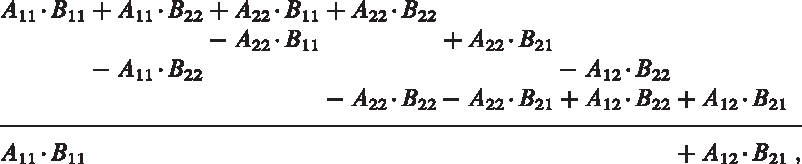
\includegraphics{算法导论第四版插图/第四章/斯特拉森算法公式.pdf}

对应了等式 (4.5)。 类似的,我们设

$$
C_{12}=C_{12}+P_1+P_2
$$

意思是更新为 $C_{12}$ 等于

$$
\frac{
    \begin{aligned}
        A_{11} \cdot B_{12} & -A_{11} \cdot B_{22} \\
        & +A_{11} \cdot B_{22}+A_{12} \cdot B_{22}
        \end{aligned}
}{A_{11} \cdot B_{12} \quad\quad\quad\;\;\quad+A_{12} \cdot B_{22}}
$$

对应了等式 (4.6)。设

$$
C_{21}=C_{21}+P_3+P_4
$$

表示更新为 $C_{21}$ 等于

$$
\frac{
    \begin{aligned}
        A_{21} \cdot B_{11} & +A_{22} \cdot B_{11} \\
        & -A_{22} \cdot B_{11}+A_{22} \cdot B_{21}
        \end{aligned}
}{
    A_{21} \cdot B_{11} \quad\quad\quad\;\;\quad+A_{22} \cdot B_{21}
}
$$

对应了等式 (4.7)。最后,设

$$
C_{22}=C_{22}+P_5+P_1-P_3-P_7
$$

表示更新为 $C_{22}$ 等于

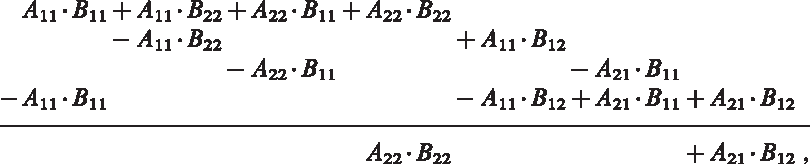
\includegraphics{算法导论第四版插图/第四章/斯特拉森公式2.pdf}

这对应于方程(4.8)。总的来说,由于在第4步中我们要进行12次$n/2\times n/2$矩阵的加减,因此该步骤确实需要$\Theta(n^2)$的时间。

我们可以看出,Strassen算法的步骤1-4使用7个子矩阵乘法和18个子矩阵加法来生成正确的矩阵乘积。我们还可以看出,递归式(4.10)描述了它的运行时间。由于第4.5节表明该递归式的解为$T(n)=\Theta(n^{\lg 7})=$ $O(n^3)$,因此Strassen方法在渐近意义下击败了$\Theta(n^3)$的MATRIX-MULTIPLY和MATRIX-MULTIPLY-RECURSIVE过程。


\section{用代入法求解递归式}\label{section-4.3}

现在你已经了解了递归式如何描述分治算法的运行时间,让我们学习如何解决它们。我们从本节开始介绍代入法,它是本章四种方法中最通用的方法。代入法包括两个步骤:

\begin{enumerate}
\item 使用符号常数猜测解的形式。
\item 使用数学归纳法来证明解有效,并找到常数。
\end{enumerate}

为了应用归纳假设,你需要在较小的值上将猜测的解代入函数中,因此称为``代入法''。这种方法很强大,但你必须猜测答案的形式。虽然生成一个好的猜测可能看起来很困难,但稍微练习一下就可以快速提高你的直觉。

你可以使用代入法来建立递归式的上界或下界。通常最好不要同时尝试进行上界和下界的证明。也就是说,不要试图直接证明$\Theta$紧密界限,而是先证明一个$O$上界,然后证明一个$\Omega$下界。它们一起给出了一个$\Theta$紧密界限(定理\ref{thm:定理3.1})。

作为代入法的例子,让我们确定递归式的渐近上界:

\begin{equation}
T(n)=2 T(\lfloor n / 2\rfloor)+\Theta(n)
\end{equation}

这个递归式类似于归并排序递归式(2.3),除了向下取整函数,它确保$T(n)$在整数上定义。让我们猜测渐近上界相同——$T(n)=O(n \lg n)$——并使用代入法来证明它。

我们将采用归纳假设$T(n) \leq c n \lg n$,其中$c>0$和$n_0>0$是特定的常数,稍后我们将看到它们需要遵守的约束条件。如果我们可以建立这个归纳假设,我们可以得出结论$T(n)=O(n \lg n)$。在讨论陷阱时,使用$T(n)=O(n \lg n)$作为归纳假设是危险的,因为常数很重要。

归纳假设假定对于所有至少大于等于$n_0$且小于$n$的数字,此界限均成立。特别地,因此如果$n \geq 2 n_0$,则对于$\lfloor n / 2\rfloor$成立,得到$T(\lfloor n / 2\rfloor) \leq c\lfloor n / 2\rfloor \lg (\lfloor n / 2\rfloor)$。将其代入递归式(4.11)——因此称为“代入”法——得到:

$$
\begin{aligned}
T(n) & \leq 2(c\lfloor n / 2\rfloor \lg (\lfloor n / 2\rfloor))+\Theta(n) \\
& \leq 2(c(n / 2) \lg (n / 2))+\Theta(n) \\
& =c n \lg (n / 2)+\Theta(n) \\
& =c n \lg n-c n \lg 2+\Theta(n) \\
& =c n \lg n-c n+\Theta(n) \\
& \leq c n \lg n,
\end{aligned}
$$

如果我们限制常数$n_0$和$c$足够大,使得对于$n \geq 2 n_0$,$c n$支配了$\Theta(n)$项中隐藏的匿名函数,则最后一步成立。

我们已经证明了归纳假设对归纳情况成立,但我们还需要证明归纳假设对归纳的基础情况也成立,即当$n_0 \leq n<2 n_0$时,$T(n) \leq c n \lg n$。只要$n_0>1$(对$n_0$的新限制),我们就有$\lg n>0$,这意味着$n \lg n>0$。因此,让我们选择$n_0=2$。由于递归式(4.11)的基本情况没有明确说明,按照惯例,$T(n)$是算法的,这意味着$T(2)$和$T(3)$是常数(如果它们描述任何实际程序在大小为2或3的输入上的最坏运行时间,则应该是常数)。选择$c=\max \{T(2), T(3)\}$得到$T(2) \leq c<(2 \lg 2) c$和$T(3) \leq c<(3 \lg 3) c$,从而建立了归纳假设的基本情况。

因此,对于所有$n \geq 2$,我们有$T(n) \leq c n \lg n$,这意味着递归式(4.11)的解是$T(n)=O(n \lg n)$。

在算法文献中,人们很少将代入证明推到这个详细的层次,尤其是在处理基本情况时。原因是对于大多数算法分治递归,基本情况都以相同的方式处理。你可以将归纳基于从方便的正常常数$n_0$到某个常数$n_0^{\prime}>n_0$的值范围上,使得对于$n \geq n_0^{\prime}$,递归总是在$n_0$和$n_0^{\prime}$之间的常量大小的基本情况中结束。(本例使用$n_0^{\prime}=2 n_0$。)然后,通常可以明显地看出,通过选择足够大的主要常数(例如本例中的$c$),归纳假设可以适用于从$n_0$到$n_0^{\prime}$的所有值。

\textbf{做出好的猜测}

不幸的是,没有通用的方法可以正确地猜测任意递归的最紧渐近解。做出好的猜测需要经验和偶尔的创造力。幸运的是,学习一些递归求解启发式方法,以及通过处理递归以获得经验,可以帮助你成为一个好的猜测者。你还可以使用递归树,在第\ref{section-4.4}节中我们将介绍它们,以帮助生成好的猜测。

如果递归类似于你以前见过的递归,则猜测类似的解是合理的。例如,考虑定义在实数上的递归式

$$
T(n)=2 T(n / 2+17)+\Theta(n)
$$

这个递归式看起来有点像归并排序递归式(2.3),但由于右侧$T$的参数中添加了``17'',所以更加复杂。然而,直觉上,这个附加项不应该对递归式的解产生实质性影响。当$n$很大时,$n / 2$和$n / 2+17$之间的相对差异并不大:两者都将$n$几乎平均分成两半。因此,猜测$T(n)=O(n \lg n)$是有道理的,你可以使用代入法验证其正确性。

另一种做出好的猜测的方法是确定递归的松散上下界,然后缩小不确定性的范围。例如,你可以从递归(4.11)的下界$T(n)=\Omega(n)$开始,因为递归包括$\Theta(n)$项,并且你可以证明一个初始的上界$T(n)=O(n^2)$。然后,将时间分配在尝试降低上界和尝试提高下界之间,直到收敛于正确的、渐近紧密的解,在这种情况下是$T(n)=\Theta(n \lg n)$。

\textbf{行业内的技巧:减去低阶项}

有时,你可能会正确猜测递归的渐近紧密界限,但是在归纳证明中却无法进行数学计算。问题通常是归纳假设不够强。解决这个问题的技巧是在遇到这种问题时通过减去低阶项来修改你的猜测。然后数学通常会得到解决。考虑定义在实数上的递归式

\begin{equation}
T(n)=2 T(n / 2)+\Theta(1)
\end{equation}

让我们猜测递归式的解为$T(n)=O(n)$并尝试展示当$n \geq n_0$时$T(n) \leq c n$,其中我们适当地选择常数$c, n_0>0$。将我们的猜测代入递归式,我们得到

$$
\begin{aligned}
T(n) & \leq 2(c(n / 2))+\Theta(1) \\
& =c n+\Theta(1)
\end{aligned}
$$

不幸的是,这并不意味着对于任何$c$的选择都有$T(n) \leq c n$。我们可能会尝试更大的猜测,比如$T(n)=O(n^2)$。虽然这个更大的猜测是正确的,但它只提供了一个松散的上界。事实证明,我们最初的猜测$T(n)=O(n)$是正确且紧密的。然而,为了证明它是正确的,我们必须加强归纳假设。

直观地说,我们的猜测几乎是正确的:我们只差了$\Theta(1)$,一个低阶项。然而,数学归纳要求我们证明归纳假设的确切形式。让我们尝试从我们以前的猜测中减去一个低阶项的技巧:$T(n) \leq c n-d$,其中$d \geq 0$是一个常数。现在我们有

$$
\begin{aligned}
T(n) & \leq 2(c(n / 2)-d)+\Theta(1) \\
& =c n-2 d+\Theta(1) \\
& \leq c n-d-(d-\Theta(1)) \\
& \leq c n-d
\end{aligned}
$$

只要我们选择的$d$大于被$\Theta$符号隐藏的匿名上界常数,就可以起作用。减去一个低阶项是可行的!当然,我们不能忘记处理基本情况,即选择足够大的常数$c$,使得$c n-d$支配隐含的基本情况。

你可能会觉得减去一个低阶项的想法有些反直觉。毕竟,如果数学无法计算,难道不应该增加猜测吗?不一定!当递归包含多个递归调用时(递归(4.12)包含两个),如果你向猜测中添加一个低阶项,则每个递归调用都会添加一次。这样做会使你远离归纳假设。另一方面,如果你从猜测中减去一个低阶项,那么你将可以为每个递归调用减去一次。在上面的例子中,我们两次减去了常数$d$,因为$T(n/2)$的系数是2。我们最终得到了不等式$T(n) \leq c n-d-(d-\Theta(1))$,并且很容易找到合适的$d$值。

\textbf{避免陷阱}

避免在代换法的归纳假设中使用渐近表示法,因为这容易出错。例如,对于递归(4.11),如果我们不明智地采用$T(n)=O(n)$作为归纳假设,我们可能会错误地“证明”$T(n)=O(n)$:

$$
\begin{aligned}
T(n) & \leq 2 \cdot O(\lfloor n / 2\rfloor)+\Theta(n) \\
& =2 \cdot O(n)+\Theta(n) \\
& =O(n) . \quad \Longleftarrow \text { 错误! }
\end{aligned}
$$

这种推理的问题在于,$O$符号隐藏的常数会发生变化。我们可以通过使用显式常数重复“证明”来揭示谬误。对于归纳假设,假设对于所有$n \geq n_0$,$T(n) \leq c n$,其中$c, n_0>0$是常数。重复不等式链中的前两个步骤得到

$$
\begin{aligned}
T(n) & \leq 2(c\lfloor n / 2\rfloor)+\Theta(n) \\
& \leq c n+\Theta(n) .
\end{aligned}
$$

现在,确实$c n+\Theta(n)=O(n)$,但是由于$\Theta(n)$隐藏的匿名函数是渐近正的,因此$O$符号隐藏的常数必须大于$c$。我们无法进行第三步以得出$c n+\Theta(n) \leq c n$,从而揭示了谬误。

在使用代换法或更一般的数学归纳时,必须小心,以使任何渐近表示法隐藏的常数在整个证明中保持一致。因此,在归纳假设中最好避免使用渐近表示法,并明确命名常数。

下面是另一种误用代换法来显示递归(4.11)的解为$T(n)=O(n)$的错误方法。我们猜测$T(n) \leq c n$,然后论证

$$
\begin{aligned}
T(n) & \leq 2(c\lfloor n / 2\rfloor)+\Theta(n) \\
& \leq c n+\Theta(n) \\
& =O(n), \quad \Longleftarrow \text { 错误! }
\end{aligned}
$$

因为$c$是一个正常数。错误的原因在于我们的目标是证明$T(n)=O(n)$,而我们的归纳假设是证明$T(n) \leq c n$。在使用代换法或任何归纳证明时,必须证明归纳假设的确切陈述。在这种情况下,我们必须明确证明$T(n) \leq c n$,以显示$T(n)=O(n)$。

\section{用递归树方法求解递归式}\label{section-4.4}

虽然你可以使用代入法来证明递归式的解是正确的,但你可能会难以想出一个好的猜测。像我们在第\ref{subsection-2.3.2}节中分析归并排序递归式时所做的那样,绘制递归树可以帮助你。在递归树中,每个节点表示递归函数调用集合中某个地方的单个子问题的成本。通常,你在树的每一层中对成本进行求和,以获得每一层的成本,然后你对所有层的成本进行求和,以确定递归所有层的总成本。但是,有时候计算总成本需要更多的创造力。

递归树最好用于产生好的猜测的直觉,然后你可以通过代入法进行验证。然而,如果你在绘制递归树和求和成本时非常细心,你可以将递归树用作递归式的解的直接证明。但是,如果你仅使用它来生成一个好的猜测,你通常可以容忍一小部分“粗心”,这可以简化数学。当你以后使用代入法验证猜测时,你的数学应该是精确的。本节演示了如何使用递归树解决递归式、生成好的猜测并获得递归式的直觉。

\textbf{一个例子}

让我们看看递归树如何为递归式

\begin{equation}
T(n)=3 T(n / 4)+\Theta(n^2)
\end{equation}

提供一个上界的解的好猜测。图\ref{fig:4-1}展示了如何为$T(n)=3 T(n / 4)+c n^2$推导递归树,其中常数$c>0$是$\Theta(n^2)$项中的上界常数。图的(a)部分显示了$T(n)$,它的(b)部分展开成一个等效的表示递归的树形图。根节点处的$c n^2$项表示递归式的顶层成本,而根节点的三个子树表示大小为$n / 4$的子问题所产生的成本。图(c)显示了将(b)部分中成本为$T(n / 4)$的每个节点进一步展开的过程。根节点的三个子节点的成本为$c(n / 4)^2$。我们继续通过按照递归式确定的组成部分将树中的每个节点展开来扩展该树。

\begin{figure}[htbp]
    \centering
    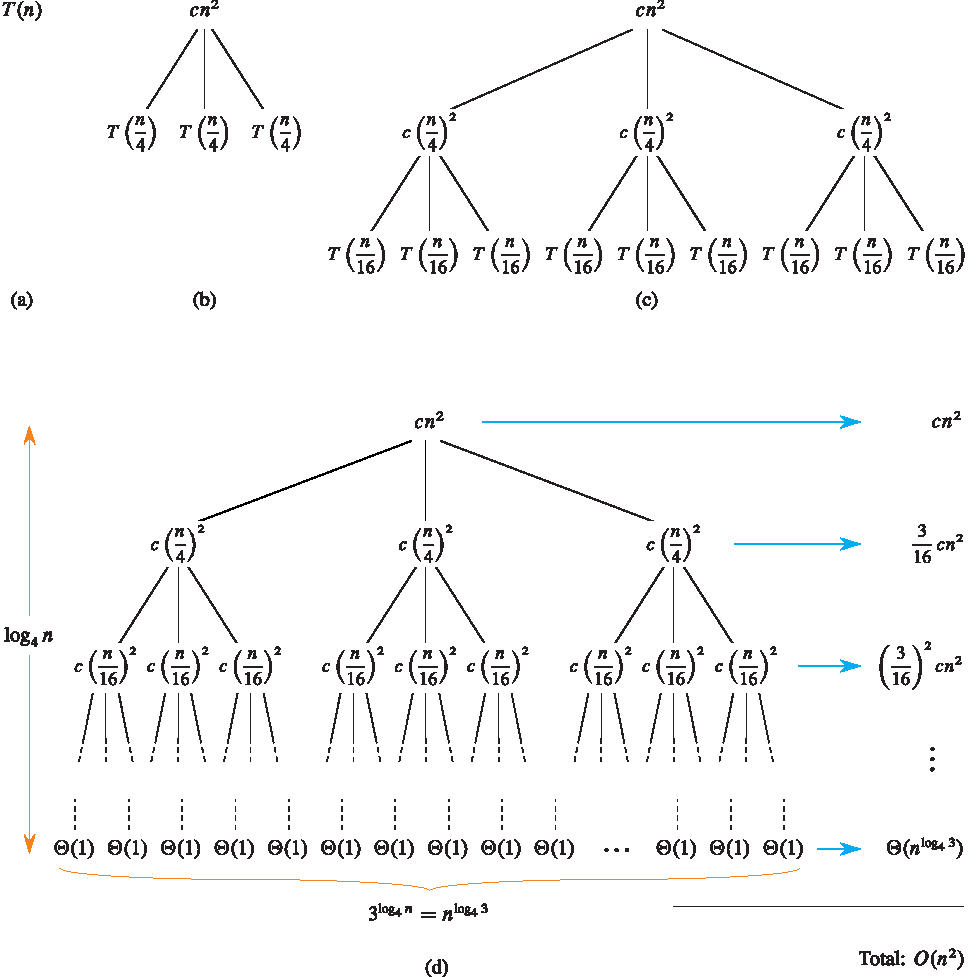
\includegraphics{算法导论第四版插图/第四章/4-1.pdf}
    \caption{为递归式$T(n)=3 T(n/4)+cn^2$构造递归树。部分(a)显示$T(n)$,它在$(\mathbf{b})-(\mathbf{d})$中逐步扩展,形成递归树。在(d)中完全展开的树的高度为$\log_4 n$。}
    \label{fig:4-1}
\end{figure}

由于每次向下一层时子问题大小减少4倍,递归必须最终在$n<n_0$的基本情况中结束。按照惯例,当$n<n_0$时,基本情况为$T(n)=\Theta(1)$,其中$n_0>0$是任何足够大以使递归式定义良好的阈值常数。然而,为了直观起见,让我们简化一下数学。假设$n$是4的精确幂,并且基本情况是$T(1)=\Theta(1)$。事实证明,这些假设不会影响渐近解。

递归树的高度是多少?深度为$i$的节点的子问题大小为$n / 4^i$。当我们从根节点向下遍历树时,当$n / 4^i=1$或等价地,当$i=\log _4 n$时,子问题大小达到$n=1$。因此,该树在深度$0,1,2,\ldots,\log _4 n-1$处具有内部节点,在深度$\log _4 n$处具有叶子节点。

图\ref{fig:4-1}的(d)部分显示了树的每一层的成本。每一层的节点数是上一层的三倍,因此深度为$i$的节点数为$3^i$。由于子问题大小在距离根越远的每个级别上减少4倍,因此深度为$i=0,1,2,\ldots,\log _4 n-1$的每个内部节点的成本为$c(n / 4^i)^2$。在相乘的过程中,我们看到给定深度$i$的所有节点的总成本为$3^ic(n / 4^i)^2=(3 / 16)^i \mathrm{cn}^2$。在最底层,在深度$\log _4 n$处,包含$3^{\log _4 n}=n^{\log _4 3}$个叶子(使用公式(3.21))。每个叶子项对总叶子成本的贡献为$\Theta(1)$,导致总叶子成本为$\Theta(n^{\log _4 3})$。

现在我们在所有层上加起来,以确定整个树的成本:

$$
\begin{aligned}
T(n) & =c n^2+\frac{3}{16} c n^2+(\frac{3}{16})^2 c n^2+\cdots+(\frac{3}{16})^{\log _4 n} c n^2+\Theta(n^{\log _4 3}) \\
& =\sum_{i=0}^{\log _4 n}(\frac{3}{16})^i c n^2+\Theta(n^{\log _4 3}) \\
& <\sum_{i=0}^{\infty}(\frac{3}{16})^i c n^2+\Theta(n^{\log _4 3}) \\
& =\frac{1}{1-(3 / 16)} c n^2+\Theta(n^{\log _4 3}) \\
& =\frac{16}{13} c n^2+\Theta(n^{\log _4 3}) \\
& =O(n^2) \quad\quad\quad\quad\quad(\Theta(n^{\log _4 3})=O(n^{0.8})=O(n^2)) .
\end{aligned}
$$

我们已经推导出递归式$T(n)=O(n^2)$的上界的解。在这个例子中,$\mathrm{cn}^2$的系数形成一个递减的几何级数。根据公式(A.7),这些系数的总和从上面受到常数$16/13$的限制。由于根节点对总成本的贡献为$\mathrm{cn}^2$,因此根节点的成本支配了整个树的总成本。

事实上,如果$O(n^2)$确实是递归式的上界的解(我们马上就会验证),那么它必须是一个紧密的上界的解。为什么?第一个递归调用会产生$\Theta(n^2)$的成本,因此$\omega(n^2)$必须是递归式的下界的解。

现在,让我们使用代换法来验证我们的猜测是否正确,即$T(n)=O(n^2)$是递归式$T(n)=3 T(n / 4)+\Theta(n^2)$的上界的解。我们想要证明存在某个常数$d>0$,使得$T(n) \leq d n^2$。使用与之前相同的常数$c>0$,我们有:

$$
\begin{aligned}
T(n) & \leq 3 T(n / 4)+c n^2 \\
& \leq 3 d(n / 4)^2+c n^2 \\
& =\frac{3}{16} d n^2+c n^2 \\
& \leq d n^2,
\end{aligned}
$$

如果我们选择$d \geq(16 / 13) c$,则最后一步成立。

对于归纳的基本情况,设$n_0>0$为充分大的阈值常数,当$n<n_0$时,递归式$T(n)=\Theta(1)$得到了很好的定义。我们可以选择足够大的$d$,使得$d$支配$\Theta$中隐藏的常数,这样$1 \leq n<n_0$时$d n^2 \geq d \geq T(n)$,从而完成基本情况的证明。

我们刚才看到的代换法证明涉及两个命名常数$c$和$d$。我们命名了$c$并用它代表$\Theta$符号隐藏的上界常数,该常数保证存在。我们不能任意选择$c$,因为它是给定的,尽管对于任何这样的$c$,任何常数$c^{\prime} \geq c$也足够。我们还命名了$d$,但我们可以自由选择任何符合我们需求的值。在这个例子中,$d$的值恰好取决于$c$的值,这是可以接受的,因为如果$c$是常数,则$d$也是常数。

\textbf{一个不规则的例子}

\begin{figure}
    \centering
    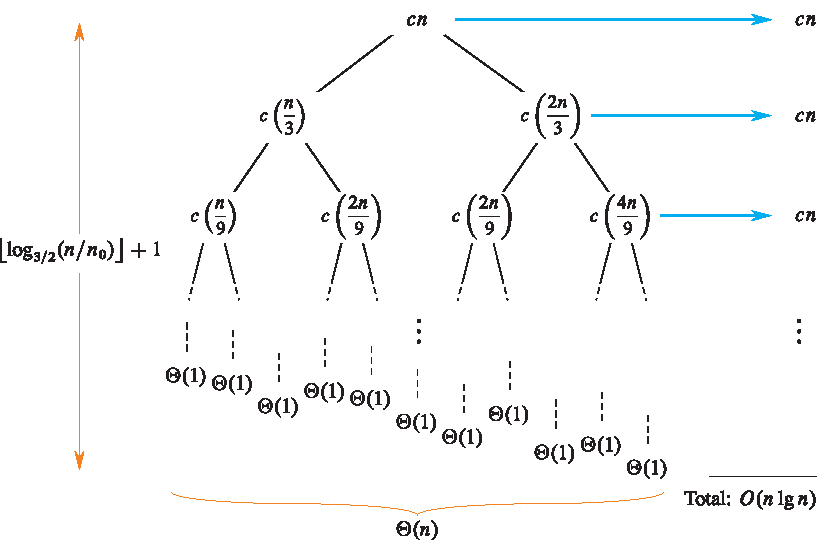
\includegraphics{算法导论第四版插图/第四章/4-2.pdf}
    \caption{递归式$T(n)=T(n / 3)+T(2 n / 3)+c n$的递归树}
    \label{fig:4-2}
\end{figure}

让我们为另一个更不规则的例子找到一个渐近上限。图\ref{fig:4-2}显示了递归式

\begin{equation}
T(n)=T(n / 3)+T(2 n / 3)+\Theta(n)
\end{equation}

的递归树。这个递归树是不平衡的,不同的根节点到叶节点的路径长度不同。在任何节点向左移动会产生一个大小为原问题的三分之一的子问题,向右移动会产生一个大小为原问题的三分之二的子问题。设$n_0>0$为隐式阈值常数,使得$0<n<n_0$时$T(n)=\Theta(1)$,并且令$c$表示$n \geq n_0$时$\Theta(n)$项隐藏的上限常数。实际上,这里有两个$n_0$常数-一个是递归中的阈值,另一个是$\Theta$符号中的阈值,因此我们将$n_0$设为这两个常数中较大的那个。

树的高度沿着树的右边缘向下,对应于大小为$n,(2 / 3) n,(4 / 9) n, \ldots, \Theta(1)$的子问题,其成本分别受到$cn,$ $c(2 n / 3)$,$c(4 n / 9), \ldots, \Theta(1)$的限制。当$(2 / 3)^h n<n_0 \leq$ $(2 / 3)^{h-1} n$时,我们到达了最右边的叶子节点,这发生在$h=\lfloor\log _{3 / 2}(n / n_0)\rfloor+1$时,因为应用方程式(3.2)中的向下取整的边界,取$x=\log _{3 / 2}(n / n_0)$,我们有$(2 / 3)^h n=$ $(2 / 3)^{\lfloor x\rfloor+1} n<(2 / 3)^x n=(n_0 / n) n=n_0$和$(2 / 3)^{h-1} n=(2 / 3)^{\lfloor x\rfloor} n>(2 / 3)^x n$ $=(n_0 / n) n=n_0$。因此,树的高度为$h=\Theta(\lg n)$。

现在我们可以理解上限了。让我们暂时不考虑叶子节点。对每个级别的内部节点的成本求和,每个级别最多有$c n$个乘以$\Theta(\lg n)$的树高度,所有内部节点的总成本为$O(n \lg n)$。

现在要处理递归树的叶子节点,它们表示基本情况,每个成本为$\Theta(1)$。有多少叶子节点?诱人的想法是将它们的数量上界定为高度为$h=\lfloor\log _{3 / 2}(n / n_0)\rfloor+1$的完全二叉树中的叶子节点数,因为递归树包含在这样一个完全二叉树中。但这种方法实际上给出了一个较差的上界。完全二叉树在根节点有1个节点,在深度1有2个节点,通常在深度$k$有$2^k$个节点。由于高度为$h=\lfloor\log _{3 / 2} n\rfloor+1$,完全二叉树中有$2^h=2^{\lfloor\log _{3 / 2} n\rfloor+1} \leq 2 n^{\log _{3 / 2} 2}$个叶子节点,这是递归树中叶子节点数的上界。由于每个叶子的成本是$\Theta(1)$,这个分析表明递归树中所有叶子的总成本是$O(n^{\log _{3 / 2} 2})=O(n^{1.71})$,这是比所有内部节点的$O(n \lg n)$成本更大的一个渐近上限。实际上,正如我们即将看到的,这个上限并不紧密。递归树中所有叶子的成本是$O(n)$-渐近小于$O(n \lg n)$。换句话说,内部节点的成本支配着叶子节点的成本,而不是相反。

与其分析叶子节点,我们现在可以停下来通过代入法证明$T(n)=\Theta(n \lg n)$。这种方法是可行的,但了解递归树有多少叶子节点是很有教益的。你可能会看到成本的递归式,其中叶子节点的成本支配着内部节点的成本,如果你有一些关于叶子节点数量分析的经验,那么你将更有把握。

为了弄清楚到底有多少叶子节点,让我们为$T(n)$的递归树中的叶子节点编写一个递归$L(n)$。由于$T(n)$中所有叶子节点都属于根节点的左子树或右子树,我们有:

\begin{equation}
L(n)= \begin{cases}1 & \text { 如果 } n<n_0 \\ L(n / 3)+L(2 n / 3) & \text { 如果 } n \geq n_0\end{cases}
\end{equation}

这个递归式与递归式(4.14)类似,但它缺少了$\Theta(n)$项,并包含了一个显式的基本情况。由于这个递归式省略了$\Theta(n)$项,因此它更容易求解。让我们应用代入法来证明它有解$L(n)=O(n)$。使用归纳假设$L(n) \leq d n$,其中$d>0$是某个常数,并假设归纳假设对小于$n$的所有值都成立,我们有:

$$
\begin{aligned}
L(n) & =L(n / 3)+L(2 n / 3) \\
& \leq d n / 3+2(d n) / 3 \\
& \leq d n,
\end{aligned}
$$

这对于任何$d>0$都成立。现在我们可以选择足够大的$d$来处理基本情况$L(n)=1$,对于$0<n<n_0$,其中$d=1$就足够了,从而完成叶子节点上限的代入法。

回到递归式(4.14)的$T(n)$,现在显然所有级别的叶子节点的总成本必须为$L(n) \cdot \Theta(1)=\Theta(n)$。由于我们已经得出了内部节点成本为$O(n \lg n)$的上限,因此递归式(4.14)的解为$T(n)=O(n \lg n)+\Theta(n)=O(n \lg n)$。

通过代入法验证递归树得出的任何上限是明智的,特别是如果你已经做出了简化假设。但是,另一种策略是使用更强大的数学方法,通常以下一节中的主方法(不幸的是不适用于递归式(4.14))或Akra-Bazzi方法(适用于该式,但需要微积分)的形式。即使你使用了强大的方法,递归树也可以提高你对在沉重的数学背景下发生了什么的直觉。

\section{用主方法求解递归式}\label{section-4.5}

主方法提供了一种“食谱”方法,用于解决形如

\begin{equation}
T(n)=aT(n/b)+f(n)
\end{equation}

的算法递归式,其中$a>0$和$b>1$是常数。我们称$f(n)$为驱动函数,称这种一般形式的递归式为主递归是。要使用主方法,你需要记住三种情况,但然后你就能够相当容易地解决许多主递归式。

主递归式描述了一种分治算法的运行时间,该算法将大小为$n$的问题分成$a$个子问题,每个子问题的大小为$n / b<n$。算法递归地解决这$a$个子问题,每个子问题的时间为$T(n / b)$。驱动函数$f(n)$包括递归之前划分问题的成本,以及将子问题的递归解合并的成本。例如,Strassen算法产生的递归是一个主递归式,其中$a=7, b=2$,驱动函数$f(n)=\Theta(n^2)$。

正如我们所提到的,在解决描述算法运行时间的递归时,我们通常更愿意忽略的一个技术细节是要求输入大小$n$是整数。例如,归并排序的运行时间可以由递归式$(2.3), T(n)=2 T(n / 2)+\Theta(n)$来描述。但是,如果$n$是奇数,我们实际上没有两个大小完全相同的问题。相反,为了确保问题大小为整数,我们将一个子问题舍入到大小$\lfloor n / 2\rfloor$,将另一个子问题舍入到大小$\lceil n / 2\rceil$,因此真正的递归式是$T(n)=T(\lceil n / 2\rceil+T(\lfloor n / 2\rfloor)+\Theta(n)$。但是,这种带有向下取整和向上取整的递归式比定义在实数上的递归式(2.3)更长更麻烦。如果不需要考虑向下取整和向上取整,我们就不考虑,特别是因为这两个递归具有相同的$\Theta(n \lg n)$解。

主方法允许你声明一个主递归式而不使用向下取整和向上取整,并隐含地推断它们。无论如何将参数舍入到最近的整数,它提供的渐近界限仍然保持不变。此外,正如我们将在第\ref{section-4.6}节中看到的那样,如果你在实数上定义主递归式而没有隐含的向下取整和向上取整,则渐近界限仍然不会改变。因此,你可以忽略主递归式中的向下取整和向上取整。第\ref{section-4.7}节给出了更一般的分治递归式中忽略向下取整和向上取整的充分条件。

\textbf{主定理}

主方法依赖下面的主定理

\begin{theorem}{主定理}{}
设$a>0$和$b>1$是常数,$f(n)$是在所有足够大的实数上定义且非负的驱动函数。定义递归式$T(n)$,其中$n \in \mathbb{N}$:
$$
T(n)=a T(n / b)+f(n)
$$
其中$a T(n / b)$实际上表示$a^{\prime} T(\lfloor n / b\rfloor)+a^{\prime \prime} T(\lceil n / b\rceil)$,其中$a^{\prime} \geq 0$和$a^{\prime \prime} \geq 0$是满足$a=a^{\prime}+a^{\prime \prime}$的常数。那么$T(n)$的渐近行为可以如下刻画:
\begin{enumerate}
\item 如果存在常数$\epsilon>0$,使得$f(n)=O(n^{\log _b a-\epsilon})$,则$T(n)=\Theta(n^{\log _b a})$。
\item 如果存在常数$k \geq 0$,使得$f(n)=\Theta(n^{\log _b a} \lg ^k n)$,则$T(n)=\Theta(n^{\log _b a} \lg ^{k+1} n)$。
\item 如果存在常数$\epsilon>0$,使得$f(n)=\Omega(n^{\log _b a+\epsilon})$,并且如果$f(n)$还满足正则条件$a f(n / b) \leq c f(n)$,其中$c<1$是某个常数,且$n$足够大,则$T(n)=\Theta(f(n))$。
\end{enumerate}
\end{theorem}

在应用主定理到一些例子之前,让我们花费一些时间来广泛理解它的含义。函数$n^{\log _b a}$被称为分水岭函数。在三种情况中,我们将驱动函数$f(n)$与分水岭函数$n^{\log _b a}$进行比较。直观地说,如果分水岭函数的增长速度渐近地比驱动函数快,那么情况1适用。如果这两个函数的渐近增长率几乎相同,则情况2适用。情况3是情况1的“相反情况”,其中驱动函数的增长速度渐近地比分水岭函数快。但是技术细节很重要。

在情况1中,分水岭函数不仅必须渐近地比驱动函数快,而且必须多项式地更快。也就是说,分水岭函数$n^{\log _b a}$必须比驱动函数$f(n)$至少快一个因子$\Theta(n^\epsilon)$,其中$\epsilon>0$是某个常数。然后,主定理说明解为$T(n)=\Theta(n^{\log _b a})$。在这种情况下,如果我们查看递归式的递归树,则每个级别的成本至少以几何级数从根到叶子增长,并且叶子节点的总成本支配内部节点的总成本。

在情况2中,分水岭和驱动函数的渐近增长率几乎相同。但更具体地说,驱动函数比分水岭函数快一个因子$\Theta(\lg^kn)$,其中$k \geq 0$。主定理说明我们要将额外的$\lg n$因子附加到$f(n)$上,得到解$T(n)=\Theta(n^{\log _b a} \lg ^{k+1} n)$。在这种情况下,递归树的每个级别的成本大致相同——$\Theta(n^{\log _b a} \lg ^k n)$——并且有$\Theta(\lg n)$个级别。在实践中,情况2最常见的情况是$k=0$,在这种情况下,分水岭和驱动函数具有相同的渐近增长率,解为$T(n)=\Theta(n^{\log _b a} \lg n)$。

情况3与情况1相似。驱动函数不仅必须渐近地比分水岭函数快,而且必须多项式地更快。也就是说,驱动函数$f(n)$必须比分水岭函数$n^{\log _b a}$至少快一个因子$\Theta(n^\epsilon)$,其中$\epsilon>0$是某个常数。此外,驱动函数必须满足正则条件$a f(n / b) \leq c f(n)$。当应用情况3时,大多数多项式有界函数都满足这个条件。如果驱动函数在局部区域增长缓慢,但整体上增长相对较快,则可能不满足正则条件。对于情况3,主定理说明解为$T(n)=\Theta(f(n))$。如果我们查看递归树,则每个级别的成本至少以几何级数从根到叶子下降,并且根的成本支配所有其他节点的成本。

值得再次看一下情况1或情况3适用的分水岭函数和驱动函数之间需要有多项式分离的要求。分离不需要很大,但必须存在,并且必须多项式增长。例如,对于递归式$T(n)=4T(n/2)+n^{1.99}$(尽管这不是分析算法时可能遇到的递归式),分水岭函数为$n^{\log _b a}=n^2$。因此,驱动函数$f(n)=n^{1.99}$相对于分水岭函数来说至少多项式小了一个因子$n^{0.01}$。因此,情况1适用,$\epsilon=0.01$。

\textbf{使用主方法}

使用主定理,你确定适用主定理的情况(如果有)并写下答案。

首先,考虑递归式$T(n)=9T(n/3)+n$。对于这个递归式,我们有$a=9$和$b=3$,这意味着$n^{\log _b a}=n^{\log _3 9}=\Theta(n^2)$。由于对于任何常数$\epsilon \leq 1$,$f(n)=n=O(n^{2-\epsilon})$,因此我们可以应用主定理的情况1得出解为$T(n)=\Theta(n^2)$。

现在考虑递归式$T(n)=T(2n/3)+1$,它具有$a=1$和$b=3/2$,这意味着分水岭函数为$n^{\log _b a}=n^{\log _{3 / 2} 1}=n^0=1$。由于$f(n)=1=\Theta(n^{\log _b a} \lg ^0 n)=\Theta(1)$,因此适用情况2。递归的解为$T(n)=\Theta(\lg n)$。

对于递归式$T(n)=3T(n/4)+n\lg n$,我们有$a=3$和$b=4$,这意味着$n^{\log _b a}=n^{\log _4 3}=O(n^{0.793})$。由于$f(n)=n \lg n=\Omega(n^{\log _4 3+\epsilon})$,其中$\epsilon$可以大约为0.2,只要正则条件对$f(n)$成立,情况3就适用。它成立,因为对于足够大的$n$,我们有$af(n/b)=3(n/4)\lg(n/4)\leq(3/4) n \lg n=c f(n)$,其中$c=3/4$。根据情况3,递归的解为$T(n)=\Theta(n\lg n)$。

接下来,让我们看看递归式$T(n)=2 T(n / 2)+n \lg n$,其中$a=2, b=2$,且$n^{\log _b a}=n^{\log _2 2}=n$。由于$f(n)=n \lg n=$ $\Theta(n^{\log _b a} \lg ^1 n)$,所以适用情况2。我们得出结论,解为$T(n)=\Theta(n \lg ^2 n)$。

我们可以使用主定理来解决第\ref{subsection-2.3.2}节、第\ref{section-4.1}节和第\ref{section-4.2}节中看到的递归式。

递归式(2.3),$T(n)=2 T(n / 2)+\Theta(n)$ 描述了归并排序的运行时间。由于$a=2$和$b=2$,分水岭函数为$n^{\log _b a}=n^{\log _2 2}=n$。由于$f(n)=\Theta(n)$,因此适用情况2,解为$T(n)=\Theta(n \lg n)$。

递归式(4.9),$T(n)=8T(n/2)+\Theta(1)$ 描述了矩阵乘法的简单递归算法的运行时间。我们有$a=8$和$b=2$,这意味着分水岭函数为$n^{\log _b a}=n^{\log _2 8}=n^3$。由于$n^3$多项式地大于驱动函数$f(n)=\Theta(1)$,实际上,对于任何正的$\epsilon<3$,我们都有$f(n)=O(n^{3-\epsilon})$,情况1适用。我们得出结论$T(n)=\Theta(n^3)$。

最后,递归式(4.10),$T(n)=7 T(n / 2)+\Theta(n^2)$,是从Strassen矩阵乘法的分析中得出的。对于这个递归式,我们有$a=7$和$b=2$,分水岭函数为$n^{\log _b a}=n^{\lg 7}$。观察到$\lg 7=2.807355 \ldots$,我们可以让$\epsilon=0.8$并限制驱动函数$f(n)=\Theta(n^2)=O(n^{\lg 7-\epsilon})$。情况1适用,解为$T(n)=\Theta(n^{\lg 7})$。

\textbf{主方法什么时候不适用}

有些情况下,你无法使用主定理。例如,分水岭函数和驱动函数可能无法渐近比较。我们可能会发现,对于无限多个$n$的值,$f(n) \gg n^{\log _b a}$,但也可能会发现,对于另外无限多个不同的$n$的值,$f(n) \ll n^{\log _b a}$。然而,在算法研究中出现的大多数驱动函数都可以与分水岭函数有意义地比较。如果你遇到一个主递归式,而情况并非如此,你将不得不使用替换或其他方法。

即使可以比较驱动函数和分水岭函数的相对增长,主定理也不能涵盖所有可能性。当$f(n)=o(n^{\log _b a})$时,在情况1和情况2之间存在一个差距,但分水岭函数并没有多项式增长得更快。同样,在情况2和情况3之间存在一个差距,当$f(n)=\omega(n^{\log _b a})$时,驱动函数增长得比分水岭函数多对数级别,但它并没有多项式增长得更快。如果驱动函数落入这些间隙之一,或者情况3中的正则条件不满足,你将需要使用主方法以外的方法来解决递归式。

作为一个驱动函数落入间隙的例子,考虑递归式$T(n)=2T(n/2)+n/\lg n$。由于$a=2$且$b=2$,分水岭函数为$n^{\log _b a}=n^{\log _2 2}=n^1=n$。驱动函数为$n / \lg n=o(n)$,这意味着它增长的速度比分水岭函数$n$慢得多。但是,$n / \lg n$只比$n$慢对数级别,而不是多项式级别。更准确地说,等式(3.24)表明,$\lg n=o(n^\epsilon)$对于任何常数$\epsilon>0$都成立,这意味着$1 / \lg n=\omega(n^{-\epsilon})$且$n / \lg n=\omega(n^{1-\epsilon})=\omega(n^{\log _b a-\epsilon})$。因此不存在任何常数$\epsilon>0$使得$n / \lg n=O(n^{\log _b a-\epsilon})$,这是情况1适用所必需的。情况2也不适用,因为$n / \lg n=\Theta(n^{\log _b a} \lg ^k n)$,其中$k=-1$,但情况2适用时$k$必须是非负的。

要解决这种递归式,必须使用其他方法,例如替换法(第4.3节)或Akra-Bazzi方法(第4.7节)。虽然主定理不能处理这种特定的递归式,但它确实可以处理在实践中经常出现的绝大多数递归式。

\section{连续主定理的证明}\label{section-4.6}

在其完整性上证明主定理(定理4.1),特别是处理向下取整和向上取整的棘手技术问题,超出了本书的范围。然而,本节陈述并证明了主定理的一个变体,称为连续主定理,其中主递归式(4.17)定义在足够大的正实数上。这个版本的证明不受向下取整和向上取整的影响,包含了理解主递归式行为所需的主要思想。第\ref{section-4.7}节更详细地讨论了分治递归中的向下取整和向上取整,提出了足够的条件,使它们不影响渐近解。

当然,由于你不需要理解主定理的证明才能应用主方法,因此你可以选择跳过本节。但是,如果你希望研究本教科书范围之外的更高级算法,则可能会欣赏对潜在数学的更好理解,连续主定理的证明提供了这种理解。

尽管我们通常假设递归式是算法性的,并且不需要明确说明基本情况,但我们必须对证明进行更加谨慎,以证明这种做法是正确的。本节中的引理和定理明确说明了基本情况,因为归纳证明需要数学基础。在数学世界中,非常小心地证明定理,以证明在实践中更加随意的做法是正确的,这是很常见的。

连续主定理的证明涉及两个引理。引理4.2使用稍微简化的主递归式,阈值常数为$n_0=1$,而不是隐含的基本情况所需的更一般的$n_0>0$阈值常数。该引理使用递归树将简化的主递归式的解减少到求和的求解方案。引理4.3为求和提供了渐近界限,反映了主定理的三种情况。最后,连续主定理本身(定理4.4)为主递归式提供了渐近界限,同时推广到任意阈值常数$n_0>0$,这是隐含的基本情况所需的。

以下是第一个引理。

\begin{lemma}{}{}
设$a>0$且$b>1$为常数,$f(n)$为定义在实数$n \geq 1$上的函数。则递归式
$$
T(n)= \begin{cases}\Theta(1) & \text { 如果 } 0 \leq n<1 \\ a T(n / b)+f(n) & \text { 如果 } n \geq 1\end{cases}
$$
有解
$$
T(n)=\Theta(n^{\log _b a})+\sum_{j=0}^{\lfloor\log _b n\rfloor} a^j f(n/b^j) .
$$
\end{lemma}

\begin{proof}
考虑图\ref{fig:4-3}中的递归树。首先看看其内部节点。树的根具有成本$f(n)$,并且它有$a$个孩子,每个孩子的成本为$f(n/b)$。(当可视化递归树时,将$a$视为整数很方便,但数学上不需要。)每个孩子都有$a$个孩子,深度为2处有$a^2$个节点,每个孩子的成本为$f(n/b^2)$。一般地,深度$j$处有$a^j$个节点,每个节点的成本为$f(n/b^j)$。

现在,我们继续理解叶子节点。树向下生长,直到$n/b^j$小于1为止。因此,树的高度为$\lfloor\log _b n\rfloor+1$,因为$n / b^{\lfloor\log _b n\rfloor} \geq n / b^{\log _b n}=1$且$n / b^{\lfloor\log _b n\rfloor+1}<n / b^{\log _b n}=1$。由于如我们所观察到的,深度$j$处的节点数为$a^j$,所有叶子节点都在深度$\lfloor\log _b n\rfloor+1$处,因此该树包含$a^{\lfloor\log _b n\rfloor+1}$个叶子节点。使用等式(3.21),我们有$a^{\lfloor\log _b n\rfloor+1} \leq a^{\log _b n+1}=a n^{\log _b a}=O(n^{\log _b a})$,因为$a$是常数,且$a^{\lfloor\log _b n\rfloor+1} \geq a^{\log _b n}=n^{\log _b a}=\Omega(n^{\log _b a})$。因此,叶子节点的总数是$\Theta(n^{\log _b a})$——渐近地,这是分界函数。

现在我们可以通过对树中每个深度的节点的成本求和来推导方程(4.18),如图所示。方程中的第一项是叶子节点的总成本。由于每个叶子节点都在深度$\lfloor\log _b n\rfloor+1$处,且$n / b^{\lfloor\log _b n\rfloor+1}<1$,递归的基本情况给出了叶子节点的成本:$T(n / b^{\lfloor\log _b n\rfloor+1})=\Theta(1)$。因此,所有$\Theta(n^{\log _b a})$个叶子节点的成本是$\Theta(n^{\log _b a}) \cdot \Theta(1)=\Theta(n^{\log _b a})$。方程(4.18)中的第二项是内部节点的成本,在基础的分治算法中,它代表将问题分解为子问题,然后重新组合子问题的成本。由于深度$j$处所有内部节点的成本均为$a^j f(n / b^j)$,所有内部节点的总成本为
$$
\sum_{j=0}^{\lfloor\log _b n\rfloor} a^j f(n / b^j)
$$
\end{proof}

\begin{figure}[htbp]
    \centering
    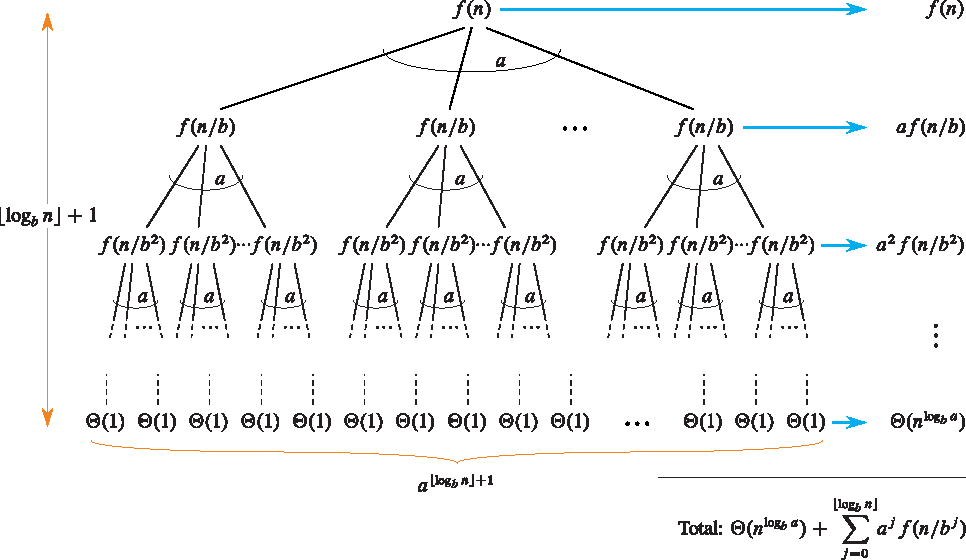
\includegraphics{算法导论第四版插图/第四章/4-3.pdf}
    \caption{$T(n)=aT(n/b)+f(n)$生成的递归树。该树是一个完全的$a$叉树,有$\lfloor a \log _b n\rfloor+1$个叶子节点和高度$\lfloor\log _b n\rfloor+1$。每个深度的节点的成本显示在右侧,并在公式(4.18)中给出它们的总和。}
    \label{fig:4-3}
\end{figure}

正如我们将要看到的,主定理的三种情况取决于递归树各层的总成本分布:

\textbf{情况1}:成本从根到叶子按几何级数增长,每一层成本都增加一个常数因子。

\textbf{情况2}:成本取决于定理中$k$的值。当$k=0$时,每一层的成本相等;当$k=1$时,从根到叶子成本线性增长;当$k=2$时,增长是二次的;一般情况下,成本在$k$中呈多项式增长。

\textbf{情况3}:成本从根到叶子按几何级数递减,每一层成本都缩小一个常数因子。

方程(4.18)中的求和描述了基础分治算法中分解和合并步骤的成本。下一个引理提供了求和增长的渐近界限。

\begin{lemma}{}{}
设$a>0$和$b>1$为常数,$f(n)$是定义在$n\geq1$的实数上的函数。则对于$n\geq1$,函数
$$
g(n)=\sum_{j=0}^{\lfloor\log _b n\rfloor} a^j f(n / b^j)
$$
的渐近行为可以如下刻画:
\begin{enumerate}
\item 若存在常数$\epsilon>0$,使得$f(n)=O(n^{\log _b a-\epsilon})$,则$g(n)=O(n^{\log _b a})$。
\item 若存在常数$k \geq 0$,使得$f(n)=\Theta(n^{\log _b a} \lg ^k n)$,则$g(n)=\Theta(n^{\log _b a} \lg ^{k+1} n)$。
\item 若存在$c$在范围$0<c<1$内,使得对于所有$n\geq1$,有$0<af(n/b) \leq cf(n)$,则$g(n)=\Theta(f(n))$。
\end{enumerate}
\end{lemma}

\begin{proof}
对于情况1,我们有$f(n)=O(n^{\log _b a-\epsilon})$,这意味着$f(n / b^j)=$ $O((n/b^j)^{\log _b a-\epsilon})$。将其代入方程(4.19)中得到

$$
\begin{aligned}
g(n) & =\sum_{j=0}^{\lfloor\log _b n\rfloor} a^j O((\frac{n}{b^j})^{\log _b a-\epsilon}) \\
& =O(\sum_{j=0}^{\lfloor\log _b n\rfloor} a^j(\frac{n}{b^j})^{\log _b a-\epsilon}) \\
& =O(n^{\log _b a-\epsilon} \sum_{j=0}^{\lfloor\log _b n\rfloor}(\frac{a b^\epsilon}{b^{\log _b a}})^j) \\
& =O(n^{\log _b a-\epsilon} \sum_{j=0}^{\lfloor\log _b n\rfloor}(b^\epsilon)^j) \\
& =O(n^{\log _b a-\epsilon}(\frac{b^{\lfloor\epsilon(\log _b n\rfloor+1)}-1}{b^\epsilon-1}))
\end{aligned}
$$

最后一个级数是等比数列。由于$b$和$\epsilon$是常数,因此$b^\epsilon-1$的分母不影响$g(n)$的渐近增长,分子中的-1也不影响。由于$b^{\epsilon(\lfloor\log _b n\rfloor+1)} \leq(b^{\log _b n+1})^\epsilon=b^\epsilon n^\epsilon=O(n^\epsilon)$,我们得到$g(n)=O(n^{\log _b a-\epsilon} \cdot O(n^\epsilon))=O(n^{\log _b a})$,从而证明了情况1。

情况2假设$f(n)=\Theta(n^{\log _b a} \lg ^k n)$,因此我们可以得出$f(n / b^j)=\Theta((n / b^j)^{\log _b a} \lg ^k(n / b^j))$。将其代入方程(4.19)中,得到

$$
\begin{aligned}
g(n) & =\Theta(\sum_{j=0}^{\lfloor\log _b n\rfloor} a^j(\frac{n}{b^j})^{\log _b a} \lg ^k(\frac{n}{b^j})) \\
& =\Theta(n^{\log _b a} \sum_{j=0}^{\lfloor\log _b n\rfloor} \frac{a^j}{b^{j \log _b a}} \lg ^k(\frac{n}{b^j})) \\
& =\Theta(n^{\log _b a} \sum_{j=0}^{\lfloor\log _b n\rfloor} \lg ^k(\frac{n}{b^j})) \\
& =\Theta(n^{\log _b a} \sum_{j=0}^{\lfloor\log _b n\rfloor}(\frac{\log _b(n / b^j)}{\log _b 2})^k) \\
& =\Theta(n^{\log _b a} \sum_{j=0}^{\lfloor\log _b n\rfloor}(\frac{\log _b n-j}{\log _b 2})^k) \\
& =\Theta(\frac{n^{\log _b a}}{\log _b^k 2} \sum_{j=0}^{\lfloor\log _b n\rfloor}(\log _b n-j)^k) \\
& =\Theta(n^{\log _b a} \sum_{j=0}^{\lfloor\log _b n\rfloor}(\log _b n-j)^k)
\end{aligned}
$$

$\Theta$符号内的求和可以如下从上界限界:

$$
\begin{aligned}
& \sum_{j=0}^{\lfloor\log _b n\rfloor}(\log _b n-j)^k \leq \sum_{j=0}^{\lfloor\log _b n\rfloor}(\lfloor\log _b n\rfloor+1-j)^k \\
& =\sum_{j=1}^{\lfloor\log _b n\rfloor+1} j^k \\
& =O((\lfloor\log _b n\rfloor+1)^{k+1}) \\
& =O(\log _b^{k+1} n) \\
&
\end{aligned}
$$

由于我们有紧密的上下界,因此这个求和是$\Theta(\log _b^{k+1} n)$,由此我们可以得出$g(n)=\Theta(n^{\log _b a} \log _b^{k+1} n)$,从而完成了情况2的证明。

对于情况3,注意到$f(n)$出现在$g(n)$的定义(当$j=0$时),并且$g(n)$的所有项都是正数。因此,我们必须有$g(n)=$ $\Omega(f n))$,只需要证明$g(n)=O(f(n))$即可。对不等式$a f(n / b) \leq c f(n)$进行$j$次迭代得到$a^j f(n / b^j) \leq c^j f(n)$。将其代入方程(4.19)中,我们得到

$$
\begin{aligned}
g(n) & =\sum_{j=0}^{\lfloor\log _b n\rfloor} a^j f(n / b^j) \\
& \leq \sum_{j=0}^{\lfloor\log _b n\rfloor} c^j f(n) \\
& \leq f(n) \sum_{j=0}^{\infty} c^j \\
& =f(n)(\frac{1}{1-c}) \\
& =O(f(n)) .
\end{aligned}
$$

因此,我们可以得出$g(n)=\Theta(f(n))$。情况3证明完成后,引理的整个证明也就完成了。
\end{proof}

现在我们可以陈述并证明连续主定理了。

\begin{theorem}{连续主定理}{}
假设$a>0$和$b>1$是常数,并且$f(n)$是在所有足够大的实数上定义且非负的驱动函数。通过以下算法递归定义正实数上的$T(n)$:
$$
T(n)=a T(n / b)+f(n)
$$
那么$T(n)$的渐近行为可以如下刻画:
\begin{enumerate}
\item 如果存在一个常数$\epsilon>0$,使得$f(n)=O(n^{\log _b a-\epsilon})$,则$T(n)=$ $\Theta(n^{\log _b a})$。
\item 如果存在一个常数$k \geq 0$,使得$f(n)=\Theta(n^{\log _b a} \lg ^k n)$,则$T(n)=$ $\Theta(n^{\log _b a} \lg ^{k+1} n)$。
\item 如果存在一个常数$\epsilon>0$,使得$f(n)=\Omega(n^{\log _b a+\epsilon})$,并且如果$f(n)$还满足正则性条件$a f(n / b) \leq c f(n)$(其中$c<1$是常数,并且$n$足够大),则$T(n)=\Theta(f(n))$。
\end{enumerate}
\end{theorem}

\begin{proof}
证明思路是通过运用引理4.3来限制引理4.2中的求和式(4.18)。但是我们必须针对$0<n<1$使用引理4.2的基本情况,而这个定理使用了一个隐含的基本情况$0<n<n_0$,其中$n_0>0$是任意的阈值常数。由于递归是算法性质的,我们可以假设$f(n)$对于$n \geq n_0$已经被定义。

对于$n>0$,让我们定义两个辅助函数$T^{\prime}(n)=T(n_0 n)$和$f^{\prime}(n)=f(n_0 n)$。我们有:

\begin{equation}
\begin{aligned}
T^{\prime}(n) & =T(n_0 n) \\
& = \begin{cases}\Theta(1) & \text { 如果 } n_0 n<n_0 \\
a T(n_0 n / b)+f(n_0 n) & \text { 如果 } n_0 n \geq n_0\end{cases} \\
& = \begin{cases}\Theta(1) & \text { 如果 } n<1, \\
a T^{\prime}(n / b)+f^{\prime}(n) & \text { 如果 } n \geq 1 .\end{cases}
\end{aligned}
\end{equation}

我们已经得到了$T^{\prime}(n)$的递归关系式,它满足引理4.2的条件,根据该引理,解为:

\begin{equation}
T^{\prime}(n)=\Theta(n^{\log _b a})+\sum_{j=0}^{\lfloor\log _b n\rfloor} a^j f^{\prime}(n / b^j)
\end{equation}

为了解决$T^{\prime}(n)$,我们首先需要限制$f^{\prime}(n)$。让我们检查定理中的各个情况。

情况1的条件是$f(n)=O(n^{\log _b a-\epsilon})$,其中$\epsilon>0$是某个常数。我们有:

$$
\begin{aligned}
f^{\prime}(n) & =f(n_0 n) \\
& =O((n_0 n)^{\log _b a-\epsilon}) \\
& =O(n^{\log _b a-\epsilon}),
\end{aligned}
$$

由于$a, b, n_0$和$\epsilon$都是常数。函数$f^{\prime}(n)$满足引理4.3的情况1的条件,而且引理4.2中方程(4.18)中的求和式计算结果为$O(n^{\log _b a})$。因为$a, b$和$n_0$都是常数,我们有:

$$
\begin{aligned}
T(n) & =T^{\prime}(n / n_0) \\
& =\Theta((n / n_0)^{\log _b a})+O((n / n_0)^{\log _b a}) \\
& =\Theta(n^{\log _b a})+O(n^{\log _b a}) \\
& =\Theta(n^{\log _b a})
\end{aligned}
$$

从而完成了定理中的情况1。

情况2的条件是$f(n)=\Theta(n^{\log _b a} \lg ^k n)$,其中$k \geq 0$是某个常数。我们有:

$$
\begin{aligned}
f^{\prime}(n) & =f(n_0 n) \\
& =\Theta((n_0 n)^{\log _b a} \lg ^k(n_0 n)) \\
& =\Theta(n^{\log _b a} \lg ^k n) \quad \text { (消除常数项) } .
\end{aligned}
$$

类似于情况1的证明,函数$f^{\prime}(n)$满足引理4.3的情况2的条件。因此,引理4.2中方程(4.18)中的求和式为$\Theta(n^{\log _b a} \lg ^{k+1} n)$,这意味着:

$$
\begin{aligned}
T(n) & =T^{\prime}(n / n_0) \\
& =\Theta((n / n_0)^{\log _b a})+\Theta((n / n_0)^{\log _b a} \lg ^{k+1}(n / n_0)) \\
& =\Theta(n^{\log _b a})+\Theta(n^{\log _b a} \lg ^{k+1} n) \\
& =\Theta(n^{\log _b a} \lg ^{k+1} n)
\end{aligned}
$$

从而证明了定理中的情况2。

最后,情况3的条件是$f(n)=\Omega(n^{\log _b a+\epsilon})$,其中$\epsilon>0$是某个常数,并且$f(n)$还满足正则条件$a f(n / b) \leq c f(n)$,其中$n \geq n_0$且$c<1$和$n_0>1$是某些常数。情况3的第一部分类似于情况1:

$$
\begin{aligned}
f^{\prime}(n) & =f(n_0 n) \\
& =\Omega((n_0 n)^{\log _b a+\epsilon}) \\
& =\Omega(n^{\log _b a+\epsilon}) .
\end{aligned}
$$

利用$f^{\prime}(n)$的定义以及$n_0 n \geq n_0$对于所有$n \geq 1$成立的事实,我们有:

$$
\begin{aligned}
a f^{\prime}(n / b) & =a f(n_0 n / b) \\
& \leq c f(n_0 n) \\
& =c f^{\prime}(n) .
\end{aligned}
$$

因此,$f^{\prime}(n)$满足引理4.3的情况3的要求,而且引理4.2中方程(4.18)中的求和式计算结果为$\Theta(f^{\prime}(n))$,得到:

$$
\begin{aligned}
T(n) & =T^{\prime}(n / n_0) \\
& =\Theta((n / n_0)^{\log _b a})+\Theta(f^{\prime}(n / n_0)) \\
& =\Theta(f^{\prime}(n / n_0)) \\
& =\Theta(f(n))
\end{aligned}
$$

这完成了定理中情况3的证明,从而完成了整个定理的证明。
\end{proof}

\section{Akra-Bazzi递归式}\label{section-4.7}

本节概述了两个与分治递归相关的高级主题。第一个处理由于使用向上取整和向下取整而产生的技术细节,第二个讨论了Akra-Bazzi方法,这涉及到一些微积分,用于解决复杂的分治递归。

特别地,我们将研究由Akra和Bazzi最初研究的算法分治递归的类。这些Akra-Bazzi递归采用以下形式:

\begin{equation}
T(n)=f(n)+\sum_{i=1}^k a_i T(n / b_i),
\end{equation}

其中$k$是正整数;所有常数$a_1, a_2, \ldots, a_k \in \mathbb{R}$都是严格正的;所有常数$b_1, b_2, \ldots, b_k \in \mathbb{R}$都严格大于1;并且驱动函数$f(n)$在足够大的非负实数上定义且本身非负。

Akra-Bazzi递归推广了主定理所涉及的递归类。虽然主递归表征将问题分解为相等大小的子问题(模除向上取整和向下取整)的分治算法的运行时间,但Akra-Bazzi递归可以描述将问题分解为不同大小的子问题的分治算法的运行时间。但是,主定理允许你忽略向上取整和向下取整,但是Akra-Bazzi方法用于解决Akra-Bazzi递归需要额外的要求来处理向上取整和向下取整。

但是,在深入了解Akra-Bazzi方法之前,让我们先了解忽略Akra-Bazzi递归中的向上取整和向下取整所涉及的限制。正如你所知,算法通常处理整数大小的输入。然而,递归的数学通常比整数更容易处理实数,因为我们必须处理向上取整和向下取整以确保项被良好定义。这种差异可能看起来并不大,特别是因为递归通常是这样的真相,但为了数学上的正确性,我们必须小心我们的假设。由于我们的最终目标是理解算法而不是数学边角情况的琐碎细节,因此我们希望既随意又严谨。我们如何在确保严谨性的同时随意地处理向上取整和向下取整?

从数学角度来看,处理向上取整和向下取整的困难在于某些驱动函数可能非常奇怪。因此,在Akra-Bazzi递归中通常不能忽略向上取整和向下取整。幸运的是,我们在算法研究中遇到的大多数驱动函数表现良好,向上取整和向下取整不会产生影响。

\textbf{多项式增长条件}

如果方程(4.22)中的驱动函数$f(n)$在以下意义上表现良好,则可以忽略向上取整和向下取整。

\begin{tcolorbox}
对于所有足够大的正实数,定义在上的函数$f(n)$满足多项式增长条件,如果存在一个常数$\hat{n}>0$,使得对于每个常数$\phi \geq 1$,存在一个常数$d>1$(取决于$\phi$),使得对于所有$1 \leq \psi \leq \phi$和$n \geq \hat{n}$,都有$f(n) / d \leq f(\psi n) \leq d f(n)$。
\end{tcolorbox}

这个定义可能是本教材中最难理解的定义之一。从一阶角度来看,它表明$f(n)$满足$f(\Theta(n))=\Theta(f(n))$的性质,尽管多项式增长条件实际上略微更强。该定义还意味着$f(n)$是渐近正的。

满足多项式增长条件的函数的例子包括任何形式为$f(n)=\Theta(n^\alpha \lg ^\beta n \lg \lg ^\gamma n)$的函数,其中$\alpha, \beta$和$\gamma$是常数。本书中使用的大多数多项式有界函数都满足此条件。指数和超指数不满足此条件,也存在不满足此条件的多项式有界函数。

\textbf{在``好的''递归中的向上取整和向下取整}

当Akra-Bazzi递归中的驱动函数满足多项式增长条件时,向上取整和向下取整不会改变解的渐近行为。下面的定理,没有给出证明,而是形式化了这个概念。

\begin{theorem}{}{}
设$T(n)$是定义在非负实数上的函数,满足递归式(4.22),其中$f(n)$满足多项式增长条件。设$T^{\prime}(n)$是另一个定义在自然数上的函数,也满足递归式(4.22),除了每个$T(n / b_i)$被替换为$T(\lceil n / b_i\rceil)$或$T(\lfloor n / b_i\rfloor)$之外。那么我们有$T^{\prime}(n)=\Theta(T(n))$。
\end{theorem}

向上取整和向下取整对递归中的参数表示一种较小的扰动。根据不等式(3.2),它们最多会使参数扰动1。但是更大的扰动是可以容忍的。只要递归(4.22)中的驱动函数$f(n)$满足多项式增长条件,那么用$T(n / b_i+h_i(n))$替换任何一个$T(n / b_i)$都不会影响渐近解,其中$|h_i(n)|=O(n / \lg ^{1+\epsilon} n)$,$\epsilon>0$为某个常数,且$n$足够大。因此,在分治算法中,除法步骤可以相对粗略,而不会影响其运行时间递归的解。

\textbf{Akra-Bazzi方法}

不出所料,Akra-Bazzi方法是为解决Akra-Bazzi递归(4.22)而开发的,根据定理4.5,它适用于存在向上取整和向下取整或更大的扰动,正如刚才所讨论的那样。该方法首先确定唯一的实数$p$,使得$\sum_{i=1}^k a_i / b_i^p=1$。这样的$p$总是存在的,因为当$p \rightarrow-\infty$时,和趋向于$\infty$;它随着$p$的增加而减小;当$p \rightarrow \infty$时,它趋向于0。然后,Akra-Bazzi方法给出递归的解:

\begin{equation}
T(n)=\Theta(n^p(1+\int_1^n \frac{f(x)}{x^{p+1}} d x))
\end{equation}

作为一个例子,考虑递归式

\begin{equation}
T(n)=T(n / 5)+T(7 n / 10)+n
\end{equation}

当我们研究一种从$n$个数字集合中选择第$i$小元素的算法时,我们将看到类似的递归(9.1)。该递归具有方程(4.22)的形式,其中$a_1=a_2=1$,$b_1=5$,$b_2=10/7$,$f(n)=n$。为了解决它,Akra-Bazzi方法指出我们应该确定唯一的$p$,满足:

$$
(\frac{1}{5})^p+(\frac{7}{10})^p=1
$$

求解$p$有点麻烦——结果$p=0.83978 \ldots$——但是我们可以在不知道$p$的确切值的情况下解决递归。注意到$(1 / 5)^0+(7 / 10)^0=2$,$(1 / 5)^1+(7 / 10)^1=9 / 10$,因此$p$在$0<p<1$范围内。这足以让Akra-Bazzi方法给出我们的解。我们将使用微积分的一个事实,即如果$k \neq-1$,则$\int x^k d x=x^{k+1} /(k+1)$,我们将应用于$k=-p \neq-1$。Akra-Bazzi解(4.23)给出

$$
\begin{aligned}
& T(n)=\Theta(n^p(1+\int_1^n \frac{f(x)}{x^{p+1}} d x)) \\
& =\Theta(n^p(1+\int_1^n x^{-p} d x)) \\
& =\Theta(n^p(1+[\frac{x^{1-p}}{1-p}]_1^n)) \\
& =\Theta(n^p(1+(\frac{n^{1-p}}{1-p}-\frac{1}{1-p}))) \\
& =\Theta(n^p \cdot \Theta(n^{1-p})) \\
& =\Theta(n) \\
&
\end{aligned}
$$

尽管Akra-Bazzi方法比主定理更通用,但它需要微积分和有时需要更多的推理。如果你要忽略向上取整和向下取整,还必须确保你的驱动函数满足多项式增长条件,尽管这很少是问题。当子问题大小更或多或少相等时,主定理更简单易用。它们都是你算法工具箱中的好工具。

\chapter{概率分析与随机算法}\label{chapter-05}

本章介绍概率分析和随机算法。

\section{雇佣问题}\label{section-5.1}

假设你需要雇用一位新的办公室助手。你之前的招聘尝试都没有成功,因此你决定使用一家就业机构。就业机构每天向你推荐一个候选人。你会面试该候选人,然后决定是否雇用他。你必须向就业机构支付一笔小费来面试申请人。实际上雇用一个申请人更加昂贵,因为你必须解雇当前的办公室助手,并向就业机构支付大量的招聘费用。你承诺始终拥有最适合工作的人。因此,你决定在面试每个申请人之后,如果该申请人比当前的办公室助手更有资格,你将解雇当前的办公室助手并雇用新的申请人。你愿意支付这种策略的结果费用,但你希望估计这种费用会是多少。

本页上的HIRE-ASSISTANT过程以伪代码表示了这种招聘策略。办公室助手工作的候选人编号为1到$n$,按照这个顺序进行面试。该过程假定在面试候选人$i$之后,你可以确定候选人$i$是否是迄今为止最优秀的候选人。它首先创建一个虚拟候选人,编号为0,该候选人的资质低于其他所有候选人。

这个问题的成本模型与第\ref{chapter-02}章中描述的模型不同。我们关注的不是HIRE-ASSISTANT的运行时间,而是面试和招聘所支付的费用。表面上,分析此算法的成本表面上,分析这个问题的成本似乎与分析归并排序的运行时间非常不同。然而,所使用的分析技术无论是分析成本还是运行时间都是相同的。在任何情况下,我们都在计算执行某些基本操作的次数。

面试的成本很低,例如$c_i$,而招聘则很昂贵,成本为$c_h$。假设一共雇用了$m$人,则与此算法相关的总成本为$O(c_i n+c_h m)$。无论你雇用多少人,你总是会面试$n$个候选人,因此总是会产生与面试相关的成本$c_i n$。因此,我们集中分析$c_h m$,即招聘成本。这个数量取决于你面试候选人的顺序。

这种情况作为一种常见的计算范例。算法通常需要通过检查序列的每个元素并维护当前的``赢家''来找到序列中的最大或最小值。招聘问题模拟了一个过程多久更新其当前获胜元素的概念。

\textbf{最坏情况分析}

在最坏的情况下,你实际上会雇用你面试的每个候选人。如果候选人按照严格递增的质量顺序到来,则会发生这种情况,此时你将雇用$n$次,总雇用成本为$O(c_h n)$。

当然,候选人并不总是按照质量递增的顺序到来。事实上,你不知道他们到达的顺序,也无法控制这个顺序。因此,自然而然地会问,在典型或平均情况下我们期望会发生什么。

\textbf{可能性分析}

概率分析是在问题分析中使用概率的方法。最常见的情况是,我们使用概率分析来分析算法的运行时间。有时我们使用它来分析其他量,例如HIRE-ASSISTANT过程中的招聘成本。为了进行概率分析,我们必须使用关于输入分布的知识或假设。然后我们分析我们的算法,计算平均情况下的运行时间,即在可能输入的分布上进行平均或期望值计算。在报告这样的运行时间时,我们称之为平均情况下的运行时间。

在决定输入分布时必须小心。对于某些问题,你可以合理地假设所有可能输入的集合,并使用概率分析作为设计高效算法的技术和获得有关问题的见解的手段。对于其他问题,你无法确定合理的输入分布,在这些情况下你无法使用概率分析。

对于招聘问题,我们可以假设申请人以随机顺序到来。对于这个问题,这意味着什么呢?我们假设你可以比较任何两个候选人并决定哪个更有资格,这就是说,候选人之间存在一个全排列。因此,你可以为每个候选人排名,从1到$n$使用rank$(i)$表示申请人$i$的排名,并采用约定,即较高的排名对应更有资格的申请人。有序列表$\langle\operatorname{rank(1)}$,$\operatorname{rank}(2)$,$\ldots$,$\operatorname{rank}(n)\rangle$是列表$\langle 1,2,\ldots,n\rangle$的排列。说申请人以随机顺序到来等价于说这个排名列表等可能地是$1$到$n$的$n$!个排列中的任何一个。或者,我们说这些排名形成一个均匀随机排列,也就是说,每个可能的$n!$个排列出现的概率相等。

第\ref{section-5.2}节包含了招聘问题的概率分析。

\textbf{随机算法}

为了使用概率分析,你需要了解有关输入分布的一些信息。在许多情况下,你对输入分布了解甚少。即使你确实了解有关分布的一些信息,你可能无法将此知识计算模型化。然而,概率和随机性经常作为算法设计和分析的工具,通过使算法的一部分表现出随机性。

在招聘问题中,似乎候选人是以随机顺序呈现给你的,但你无法知道他们是否真的是这样。因此,为了为招聘问题开发随机化算法,你需要更多地控制你面试候选人的顺序。因此,我们将略微改变模型。就业机构提前向你发送$n$个候选人的列表。每天,你随机选择要面试的候选人。虽然你对候选人一无所知(除了他们的姓名),但我们已经做出了重大改变。你没有接受就业机构给你的顺序并希望它是随机的,而是获得了控制过程并强制执行随机顺序。

更一般地说,如果算法的行为不仅由其输入确定,而且还由随机数生成器产生的值确定,则称该算法为随机化算法。我们假设我们可以使用随机数生成器RANDOM。调用RANDOM$(a,b)$将返回一个整数,该整数在$a$和$b$之间(包括$a$和$b$),每个这样的整数具有相等的可能性。例如,RANDOM$(0,1)$以$1/2$的概率产生0,并以$1/2$的概率产生1。调用RANDOM$(3,7)$返回$3,4,5,6$或7中的任何一个,每个整数的概率为$1/5$。RANDOM返回的每个整数都独立于先前调用返回的整数。你可以将RANDOM想象为掷一个$(b-a+1)$面的骰子来获取其输出。(在实践中,大多数编程环境提供伪随机数生成器:一种返回``看起来''统计上随机的数字的确定性算法。)

在分析随机算法的运行时间时,我们将运行时间的期望值取自由随机数生成器返回的值的分布。我们通过将随机化算法的运行时间称为期望运行时间来将这些算法与输入为随机的算法区分开来。通常,在概率分布涉及算法输入时,我们讨论平均情况下的运行时间,而在算法本身进行随机选择时,我们讨论期望运行时间。

\section{指示器随机变量}\label{section-5.2}

为了分析许多算法,包括聘用问题,我们使用指示随机变量。指示随机变量提供了在概率和期望之间转换的便捷方法。给定样本空间$S$和事件$A$,与事件$A$相关联的指示随机变量$\mathrm{I}\{A\}$定义为:

$$
\mathrm{I}\{A\}= \begin{cases}1 & \text { 如果 } A \text { 出现 } \\ 0 & \text { 如果 } A \text { 没有出现 } .\end{cases}
$$

作为一个简单的例子,让我们确定掷一枚公平硬币时获得正面的期望次数。单次硬币抛掷的样本空间为$S=\{H, T\}$,其中$\operatorname{Pr}\{H\}=\operatorname{Pr}\{T\}=1 / 2$。我们可以定义与硬币出现正面事件$H$相关联的指示随机变量$X_H$。此变量计算本次抛掷中获得的正面次数,如果硬币出现正面,则为1,否则为0。我们写成:

$$
\begin{aligned}
X_H & =\mathrm{I}\{H\} \\
& = \begin{cases}1 & \text { 如果 } H \text { 出现 }, \\
0 & \text { 如果 } T \text { 出现 } .\end{cases}
\end{aligned}
$$

在一次抛掷硬币中获得正面的期望次数就是我们的指示变量$X_H$的期望值:

$$
\begin{aligned}
\mathrm{E}[X_H] & =\mathrm{E}[\mathrm{I}\{H\}] \\
& =1 \cdot \operatorname{Pr}\{H\}+0 \cdot \operatorname{Pr}\{T\} \\
& =1 \cdot(1 / 2)+0 \cdot(1 / 2) \\
& =1 / 2 .
\end{aligned}
$$

因此,抛一次公正硬币所得到的正面期望数量为$1/2$。如下引理所示,与事件$A$相关联的指示随机变量的期望值等于$A$发生的概率。

\begin{lemma}{}{}
给定样本空间$S$和样本空间$S$中的事件$A$,令$X_A=\mathrm{I}\{A\}$。则$\mathrm{E}[X_A]=\operatorname{Pr}\{A\}$。
\end{lemma}

\begin{proof}
证明根据方程(5.1)中指示随机变量的定义和期望值的定义,我们有

$$
\begin{aligned}
\mathrm{E}[X_A] & =\mathrm{E}[\mathrm{I}\{A\}] \\
& =1 \cdot \operatorname{Pr}\{A\}+0 \cdot \operatorname{Pr}\{\bar{A}\} \\
& =\operatorname{Pr}\{A\},
\end{aligned}
$$

$$
\text { 其中 } \bar{A} \text { 表示 } S-A \text {, 也就是 } A \text { 的补集。}
$$
\end{proof}

虽然对于像计算单次抛掷硬币的正面期望次数这样的应用,指示随机变量可能看起来很繁琐,但它们对于分析执行重复随机试验的情况非常有用。例如,在附录$\mathrm{C}$中,指示随机变量提供了一种简单的方法来确定$n$次硬币抛掷中正面朝上的期望次数。一种选择是将获得0个正面、1个正面、2个正面等的概率分别考虑,以得到等式(C.41)的结果。或者,我们可以采用方程(C.42)提出的更简单的方法,该方法隐含地使用了指示随机变量。更明确地说明这一点,让$X_i$成为与第$i$次抛掷出现正面事件相关联的指示随机变量:$X_i=\mathrm{I}$第$i$次抛掷结果为事件$\{H\}$。让$X$成为表示$n$次硬币抛掷中总正面次数的随机变量,这样

$$
X=\sum_{i=1}^n X_i
$$

为了计算正面朝上的期望次数,需要对上述方程两边取期望,得到

$$
\mathrm{E}[X]=\mathrm{E}[\sum_{i=1}^n X_i]
$$

根据引理5.1,每个随机变量的期望值为$\mathrm{E}[X_i]=1 / 2$,其中$i=1,2, \ldots, n$。然后我们可以计算期望值之和:$\sum_{i=1}^n \mathrm{E}[X_i]=n / 2$。但是等式(5.2)要求的是总和的期望值,而不是期望值之和。我们该如何解决这个难题?期望的线性性,即等式(C.24),可以解决这个问题:总和的期望值总是等于期望值之和。即使在随机变量之间存在依赖关系时,期望的线性性也适用。将指示随机变量与期望的线性性相结合,可以为我们计算多个事件发生时的期望值提供强大的技巧。现在我们可以计算正面朝上的期望次数:

$$
\begin{aligned}
\mathrm{E}[X] & =\mathrm{E}[\sum_{i=1}^n X_i] \\
& =\sum_{i=1}^n \mathrm{E}[X_i] \\
& =\sum_{i=1}^n 1 / 2 \\
& =n / 2
\end{aligned}
$$

因此,与等式(C.41)中使用的方法相比,指示随机变量极大地简化了计算。我们在整本书中都使用指示随机变量。

\textbf{使用指示随机变量分析聘用问题}

回到聘用问题,我们现在希望计算你聘用新办公助手的次数的期望值。为了使用概率分析,让我们假设候选人以随机顺序到达,如第5.1节所讨论的那样。(我们将在第5.3节中看到如何消除这个假设。)让$X$成为其值等于你聘用新办公助手次数的随机变量。然后我们可以应用等式(C.23)中的期望值定义来获得:

$$
\mathrm{E}[X]=\sum_{x=1}^n x \operatorname{Pr}\{X=x\}
$$

但是这个计算会很繁琐。相反,让我们通过使用指示随机变量来简化计算。

为了使用指示随机变量,不要仅定义一个变量表示你聘用新办公助手的次数来计算$\mathrm{E}[X]$,而是将聘用过程视为重复的随机试验,并定义$n$个变量,表示每个特定候选人是否被聘用。具体而言,让$X_i$成为与第$i$个候选人被聘用事件相关联的指示随机变量。因此,

$$
\begin{aligned}
X_i & =\mathrm{I} \{\text { 候选人 } i \text { 被聘用 }\} \\
& = \begin{cases}1 & \text { 如果候选人 } i \text { 被聘用 }, \\
0 & \text { 如果候选人 } i \text { 未被聘用 },\end{cases}
\end{aligned}
$$

以及

$$
X=X_1+X_2+\cdots+X_n
$$

引理 5.1 给出了

$$
\{\mathrm{E}[X_i]=\operatorname{Pr} \text { candidate } i \text { is hired }\}
$$

因此,我们必须计算HIRE-ASSISTANT的第5-6行被执行的概率。

当且仅当候选人$i$比候选人1到$i-1$中的每个人都更好时,候选人$i$才会在第6行被聘用。因为我们假设候选人以随机顺序到达,所以前$i$个候选人以随机顺序出现。这前$i$个候选人中的任何一个都有同等的可能性成为迄今为止最合格的人。候选人$i$有$1/i$的概率比候选人1到$i-1$更合适,因此有$1/i$的概率被聘用。根据引理5.1,我们得出结论:

$$
\mathrm{E}[X_i]=1 / i
$$

现在我们可以计算 $\mathrm{E}[X]$ :

$$
\begin{array}{rlr}
\mathrm{E}[X] & =\mathrm{E}[\sum_{i=1}^n X_i] &  \\
& =\sum_{i=1}^n \mathrm{E}[X_i] &  \\
& =\sum_{i=1}^n \frac{1}{i} &  \\
& =\ln n+O(1) & 
\end{array}
$$

即使你面试了$n$个人,平均而言,你实际上只聘用了大约$\ln n$个人。我们将这个结果总结在以下引理中。

\begin{lemma}{}{}
假设候选人以随机顺序呈现,算法HIRE-ASSISTANT的平均情况下的总雇佣成本为$O(c_h \ln n)$。
\end{lemma}

\begin{proof}
这个界限立即从我们对聘用成本的定义和方程(5.6)中得出,方程显示聘用的期望次数大约为$\ln n$。
\end{proof}

平均情况下的聘用成本相对于最坏情况下的$O(c_h n)$聘用成本是一个显著的改进。

\section{随机算法}\label{section-5.3}

在前一节中,我们展示了了解输入分布如何帮助我们分析算法的平均情况行为。如果你不知道分布怎么办?那么你就无法进行平均情况分析。然而,如第\ref{section-5.1}节所述,你可能能够使用随机化算法。

对于像招聘问题这样的问题,假设输入的所有排列是等可能的是有帮助的,概率分析可以指导我们开发随机化算法。我们不是假设输入的分布,而是强制执行分布。特别地,在运行算法之前,让我们随机排列候选人,以强制实施每个排列等可能的属性。虽然我们已经修改了算法,但我们仍然期望大约聘请新办公助理$\ln n$次。但现在我们期望这对于任何输入都是如此,而不是对于从特定分布中提取的输入。

让我们进一步探讨概率分析和随机化算法之间的区别。在第\ref{section-5.2}节中,我们声称,在假设候选人以随机顺序到达的情况下,聘请新办公助理的预期次数约为$\ln n$。该算法是确定性的:对于任何特定输入,聘请新办公助理的次数始终相同。此外,聘请新办公助理的次数因不同输入而异,并且取决于各候选人的排名。由于此数字仅取决于候选人的排名,因此为了表示特定输入,我们可以按顺序列出候选人的排名$\langle\operatorname{rank}(1),\operatorname{rank}(2),\ldots,\operatorname{rank}(n)\rangle$。给定排名列表$A_1=\langle 1,2,3,4,5,6,7,8,9,10\rangle$,新办公助理总是被聘请10次,因为每个连续的候选人都比前一个更好,并且在每次迭代中都会执行HIRE-ASSISTANT的第5-6行。给定排名列表$A_2=\langle 10,9,8,7,6,5,4,3,2,1\rangle$,只有在第一次迭代中才会聘请新办公助理。给定排名列表$A_3=\langle 5,2,1,8,4,7,10,9,3,6\rangle$,将聘请三次新办公助理,即面试排名为5、8和10的候选人。回想一下,我们算法的成本取决于你聘请新办公助理的次数,因此我们可以看到存在昂贵的输入(例如$A_1$),廉价的输入(例如$A_2$)和中等昂贵的输入(例如$A_3$)。

另一方面,考虑随机化算法,该算法首先对候选人列表进行排列,然后确定最佳候选人。在这种情况下,我们在算法中随机化,而不是在输入分布中随机化。给定特定的输入,例如上面的$A_3$,我们无法确定最大值被更新的次数,因为这个数量在每次运行算法时都不同。第一次在$A_3$上运行算法时,它可能会生成排列$A_1$并执行10次更新。但是第二次运行算法时,它可能会生成排列$A_2$并仅执行一次更新。第三次运行算法时,它可能执行其他数量的更新。每次运行算法时,其执行取决于所做的随机选择,并且很可能与算法的先前执行不同。对于该算法和许多其他随机化算法,没有特定的输入会引起其最坏情况的行为。即使你最坏的敌人也不能产生一个糟糕的输入数组,因为随机排列使输入顺序无关紧要。仅当随机数生成器产生“不幸”的排列时,随机化算法才表现不佳。

对于招聘问题,在代码中唯一需要更改的是随机排列数组,就像在RANDOMIZED-HIRE-ASSISTANT过程中所做的那样。这个简单的变化创建了一个随机化算法,其性能与假设候选人按随机顺序呈现所获得的性能相匹配。

\begin{lemma}{}{}
随机雇佣助手程序的期望雇佣成本是$O(c_h \ln n)$。
\end{lemma}

\begin{proof}
重新排列输入数组可以实现与第5.2节中HIRE-ASSISTANT的概率分析完全相同的情况。

通过仔细比较引理5.2和5.3,你可以看到概率分析和随机算法之间的区别。引理5.2对输入进行了假设。引理5.3没有这样的假设,尽管随机化输入需要一些额外的时间。为了保持一致的术语,我们将引理5.2表述为平均雇佣成本,将引理5.3表述为期望雇佣成本。在本节的其余部分,我们将讨论随机排列输入涉及的一些问题。
\end{proof}

\textbf{随机排列数组}

许多随机算法通过对给定的输入数组进行排列来随机化输入。本书的其他地方将介绍其他随机化算法,但现在,让我们看看如何随机排列$n$个元素的数组。目标是产生一个均匀随机排列,即一个与任何其他排列一样可能的排列。由于有$n!$种可能的排列,我们希望任何特定排列被产生的概率为$1/n!$。

你可能认为,要证明排列是均匀随机排列,只需证明对于每个元素$A[i]$,元素最终在位置$j$的概率为$1/n$即可。

我们的生成随机排列的方法在原地对数组进行排列:输入数组的最多一定数量的元素会被存储在数组外。过程RANDOMLY-PERMUTE在$\Theta(n)$时间内就可以原地排列数组$A[1:n]$。在第$i$次迭代中,它从元素$A[i]$到$A[n]$中随机选择元素$A[i]$。在第$i$次迭代之后,$A[i]$不再改变。

我们使用循环不变式来证明过程RANDOMLY-PERMUTE生成均匀随机排列。对于一个$n$个元素的集合,一个$k$-排列是一个包含$k$个$n$个元素中的序列,没有重复项。有$n!/(n-k)$!种可能的$k$-排列。

\begin{lemma}{}{}
过程RANDOMLY-PERMUTE计算均匀随机排列。
\end{lemma}

\begin{proof}
我们使用以下循环不变式:

在第1-2行的for循环的第$i$次迭代之前,对于$n$个元素的每个可能的$(i-1)$-排列,子数组$A[1:i-1]$以$(n-i+1)!/n!$的概率包含这个$(i-1)$-排列。

我们需要证明这个不变式在第一次循环迭代之前是正确的,每次循环迭代都保持不变式,循环终止,并且在循环终止时不变式提供了一个有用的属性来证明正确性。

初始化:考虑在第一次循环迭代之前的情况,因此$i=1$。循环不变式表示,对于每个可能的0-排列,子数组$A[1:0]$以$(n-i+1)!/n!=n!/n!=1$的概率包含这个0-排列。子数组$A[1:0]$是一个空子数组,而0-排列没有元素。因此,$A[1:0]$以1的概率包含任何0-排列,并且循环不变式在第一次迭代之前成立。

保持不变式:根据循环不变式,我们假设在第$i$次迭代之前,每个可能的$(i-1)$ -排列以$(n-i+1)!/n!$的概率出现在子数组$A[1:i-1]$中。我们将展示在第$i$次迭代后,每个可能的$i$-排列以$(n-i)!/n!$的概率出现在子数组$A[1:i]$中。然后增加$i$以进行下一次迭代,以保持循环不变式。

让我们来看看第$i$次迭代。考虑一个特定的$i$-排列,并用$\langle x_1,x_2,\ldots,x_i\rangle$表示其中的元素。这个排列由一个$(i-1)$-排列$\langle x_1,\ldots,x_{i-1}\rangle$和算法放置在$A[i]$中的值$x_i$组成。让$E_1$表示前$i-1$次迭代在$A[1:i-1]$中创建了特定的$(i-1)$-排列$\langle x_1,\ldots,x_{i-1}\rangle$的事件。根据循环不变式,$\operatorname{Pr}\{E_1\}=(n-i+1)!/n!$。让$E_2$表示第$i$次迭代将$x_i$放在位置$A[i]$的事件。当且仅当$E_1$和$E_2$同时发生时,$i$-排列$\langle x_1,\ldots,x_i\rangle$才会出现在$A[1:i]$中,因此我们希望计算$\operatorname{Pr}\{E_2 \cap E_1\}$。使用等式(C.16),我们有:

$$
\operatorname{Pr}\{E_2 \cap E_1\}=\operatorname{Pr}\{E_2 \mid E_1\} \operatorname{Pr}\{E_1\}
$$

概率$\operatorname{Pr}\{E_2 \mid E_1\}$等于$1/(n-i+1)$,因为在第2行中,算法从$A[i:n]$位置中的$n-i+1$个值中随机选择$x_i$。因此,我们有:

$$
\begin{aligned}
\operatorname{Pr}\{E_2 \cap E_1\} & =\operatorname{Pr}\{E_2 \mid E_1\} \operatorname{Pr}\{E_1\} \\
& =\frac{1}{n-i+1} \cdot \frac{(n-i+1) !}{n !} \\
& =\frac{(n-i) !}{n !} .
\end{aligned}
$$

终止:循环终止,因为它是一个迭代$n$次的for循环。在终止时,$i=n+1$,我们有子数组$A[1:n]$是一个给定的$n$-排列,概率为$(n-(n+1)+1)!/n!=0!/n!=1/n!$。

因此,RANDOMLY-PERMUTE产生了一个均匀随机排列。
\end{proof}

随机化算法通常是解决问题最简单、最有效的方法。

\section{概率分析和指示器随机变量的进一步使用}\label{section-5.4}

这个高级部分通过四个例子进一步说明了概率分析。第一个例子确定了在一个有$k$个人的房间里,其中两个人有相同的生日的概率。第二个例子研究了将球随机投掷到箱子中时会发生什么。第三个例子调查了抛硬币时连续正面的“连胜”情况。最后一个例子分析了一个招聘问题的变体,在这个问题中你必须在没有实际面试所有候选人的情况下做出决策。

\subsection{生日悖论}

我们的第一个例子是生日悖论。在一个房间里,必须有多少人才有50\%的概率其中两个人是同一年的同一天出生的?答案非常少。悖论在于,实际上比一年中的天数甚至比一年中天数的一半还要少,我们将看到这一点。

为了回答这个问题,我们用整数$1,2,\ldots,k$对房间里的人进行编号,其中$k$是房间里的人数。我们忽略闰年问题,并假设所有年份都有$n=365$天。对于$i=1,2,\ldots,k$,让$b_i$表示第$i$个人的生日是哪一天,其中$1\leq b_i\leq n$。我们还假设生日在一年中$n$天内均匀分布,因此对于$i=1,2,\ldots,k$和$r=1,2,\ldots,n$,$\operatorname{Pr}\{b_i=r\}=1/n$。

给定两个人$i$和$j$,他们具有相同生日的概率取决于随机选择生日是否独立。从现在开始,我们假设生日是独立的,因此$i$和$j$的生日都落在第$r$天的概率为:

$$
\begin{aligned}
\operatorname{Pr}\{b_i=r \text { and } b_j=r\} & =\operatorname{Pr}\{b_i=r\} \operatorname{Pr}\{b_j=r\} \\
& =\frac{1}{n^2}
\end{aligned}
$$

所以他们落到同一天过生日的概率是

$$
\begin{aligned}
\operatorname{Pr}\{b_i=b_j\}=\sum_{r=1}^n \operatorname{Pr}\{b_i=r \text { and } b_j=r\} \\
& =\sum_{r=1}^n \frac{1}{n^2} \\
& =\frac{1}{n} .
\end{aligned}
$$

更直观地说,一旦确定了$b_i$,$b_j$被选为同一天的概率为$1/n$。只要生日是独立的,$i$和$j$生日相同的概率就等于它们中任何一个人的生日恰好落在给定的一天的概率。

我们可以通过考虑补集事件来分析$k$个人中至少有2人生日相同的概率。至少有两个生日相同的概率等于所有生日都不同的概率取反。事件$B_k$表示$k$个人有不同的生日,其概率为:

$$
B_k=\bigcap_{i=1}^k A_i
$$

其中$A_i$是事件,表示对于所有$j<i$,第$i$个人的生日与第$j$个人的生日不同。由于我们可以写成$B_k=A_k\cap B_{k-1}$,因此从(C.18)得到递归式:

$$
\operatorname{Pr}\{B_k\}=\operatorname{Pr}\{B_{k-1}\} \operatorname{Pr}\{A_k \mid B_{k-1}\}
$$

我们将$\operatorname{Pr}\{B_1\}=\operatorname{Pr}\{A_1\}=1$作为初始条件。换句话说,$b_1,$ $b_2,$ $\ldots,$ $b_k$都是不同生日的概率等于$b_1,$ $b_2,$ $\ldots,$ $b_{k-1}$都是不同生日的概率乘以给定$b_1, b_2, \ldots, b_{k-1}$都是不同生日的条件下$b_k \neq b_i$($i=1,2,\ldots,k-1$)的概率。

如果$b_1, b_2, \ldots, b_{k-1}$都是不同生日,那么$b_k \neq b_i$($i=1,2,\ldots,k-1$)的条件概率是$\operatorname{Pr}\{A_k \mid B_{k-1}\}=(n-k+1)/n$,因为在$n$天中,有$n-(k-1)$天没有被占用。我们迭代地应用递归式(5.8)得到:

$$
\begin{aligned}
\operatorname{Pr}\{B_k\} & =\operatorname{Pr}\{B_{k-1}\} \operatorname{Pr}\{A_k \mid B_{k-1}\} \\
& =\operatorname{Pr}\{B_{k-2}\} \operatorname{Pr}\{A_{k-1} \mid B_{k-2}\} \operatorname{Pr}\{A_k \mid B_{k-1}\} \\
& \vdots \\
& =\operatorname{Pr}\{B_1\} \operatorname{Pr}\{A_2 \mid B_1\} \operatorname{Pr}\{A_3 \mid B_2\} \cdots \operatorname{Pr}\{A_k \mid B_{k-1}\} \\
& =1 \cdot(\frac{n-1}{n})(\frac{n-2}{n}) \cdots(\frac{n-k+1}{n}) \\
& =1 \cdot(1-\frac{1}{n})(1-\frac{2}{n}) \cdots(1-\frac{k-1}{n}) .
\end{aligned}
$$

不等式 (3.14) $1+x \leq e^x$ 告诉我们

$$
\begin{aligned}
\operatorname{Pr}\{B_k\} & \leq e^{-1 / n} e^{-2 / n} \cdots e^{-(k-1) / n} \\
& =e^{-\sum_{i=1}^{k-1} i / n} \\
& =e^{-k(k-1) / 2 n} \\
& \leq \frac{1}{2}
\end{aligned}
$$

当$-k(k-1)/2n\leq \ln(1/2)$时,所有$k$个生日都不同的概率最多为$1/2$,当$k(k-1)\geq 2n\ln 2$或通过解二次方程得到$k\geq(1+\sqrt{1+(8\ln 2)n})/2$时成立。对于$n=365$,我们必须有$k\geq 23$。因此,如果一个房间里至少有23个人,那么至少有两个人生日相同的概率就是$1/2$。由于火星一年有669个火星日,因此需要31个火星人才能达到相同的效果。

\textbf{使用指示器随机变量的分析}

指示器随机变量可以对生日悖论进行更简单但是近似的分析。对于房间里的$k$个人中的每一对$(i,j)$,定义指示器随机变量$X_{ij}$,其中$1\leq i<j\leq k$:

$$
\begin{aligned}
X_{i j} & =\mathrm{I} \{\text { 人 } i \text { 和人 } j \text { 生日相同 }\} \\
& = \begin{cases}1 & \text { 如果人 } i \text { 和人 } j \text { 生日相同 } \\
0 & \text { 其它情况。 }\end{cases}
\end{aligned}
$$

根据式子(5.7),两个人生日相同的概率为$1/n$,因此根据引理5.1,我们有:

$$
\begin{aligned}
\mathrm{E}[X_{i j}] & =\operatorname{Pr}\{\text { 人 } i \text { 和人 } j \text { 生日相同 }\} \\
& =1 / n .
\end{aligned}
$$

设$X$是计算生日相同的人对数的随机变量,我们有:

$$
X=\sum_{i=1}^{k-1} \sum_{j=i+1}^k X_{i j}
$$

对两边取期望并应用期望的线性性,我们得到:

$$
\begin{aligned}
\mathrm{E}[X] & =\mathrm{E}[\sum_{i=1}^{k-1} \sum_{j=i+1}^k X_{i j}] \\
& =\sum_{i=1}^{k-1} \sum_{j=i+1}^k \mathrm{E}[X_{i j}]
\end{aligned}
$$

$$
\begin{aligned}
& =(\begin{array}{l}
k \\
2
\end{array}) \frac{1}{n} \\
& =\frac{k(k-1)}{2 n} .
\end{aligned}
$$

当$k(k-1)\geq 2n$时,期望的生日相同的人的对数至少为1。因此,如果一个房间里至少有$\sqrt{2n}+1$个人,我们可以期望至少有两个人生日相同。对于$n=365$,如果$k=28$,则期望的生日相同的人的对数为$(28\cdot 27)/(2\cdot 365)\approx 1.0356$。因此,至少需要28个人,我们才能期望找到至少一对生日相同的人。在火星上,一年有669天,我们需要至少38个火星人。

第一次分析仅使用概率确定了存在生日相同的一对人所需的人数超过$1/2$,而第二次分析使用指示器随机变量确定了使期望的生日相同的人的对数为1的人数。虽然两种情况下所需的确切人数不同,但它们在渐近意义下是相同的:$\Theta(\sqrt{n})$。

\subsection{球和箱子}

考虑一个过程,在这个过程中,你随机地投掷相同的球进入编号为$1,2,\ldots,b$的$ b $个箱子中。投掷是独立的,每次投掷时,球同等可能地落入任何一个箱子中。被投掷的球落入任何给定箱子的概率为$1/b$。如果我们将投球过程视为Bernoulli试验序列(请参见附录C.4),其中成功意味着球落在给定的箱子中,则每次试验成功的概率为$1/b$。这个模型特别适用于分析哈希(请参见第\ref{chapter-11}章),我们可以回答关于投球过程的各种有趣问题。

\begin{itemize}
\item 有多少个球掉进了给定的箱子?掉进给定箱子的球的数量遵循二项分布$b(k;n,1/b)$。如果你投掷$n$个球,第1199页的方程式(C.41)告诉我们,掉进给定箱子的球的期望数量为$n/b$。
\item 平均而言,你需要投掷多少个球,才能让一个给定的箱子里面有一个球?直到给定箱子接收到一个球的投掷次数遵循几何分布,概率为$1/b$,根据第1197页的方程式(C.36),直到成功的期望投掷次数为$1/(1/b)=b$。
\item 你需要投掷多少个球,才能让每个箱子都至少有一个球?我们称一个球落入空箱的投掷为“命中”。我们想知道需要投掷$n$次才能得到$b$次命中的期望次数。
\end{itemize}

利用命中数,我们可以将$n$次投掷划分为多个阶段。第$i$个阶段由第$(i-1)$次命中后到第$i$次命中的投掷组成。第一个阶段包括第一次投掷,因为当所有箱子都是空的时候,你保证会有一次命中。在第$i$个阶段的每次投掷中,有$i-1$个箱子里面有球,$b-i+1$个箱子是空的。因此,在第$i$个阶段的每次投掷中,获得命中的概率为$(b-i+1)/b$。

设$n_i$表示第$i$个阶段的投掷次数,则需要得到$b$次命中的投掷次数为$n=\sum_{i=1}^b n_i$。每个随机变量$n_i$都具有概率为$(b-i+1)/b$的几何分布,因此,根据方程式(C.36),我们有:

$$
\mathrm{E}[n_i]=\frac{b}{b-i+1}
$$

根据期望的线性性质,我们有

$$
\begin{array}{rlr}
\mathrm{E}[n] & =\mathrm{E}[\sum_{i=1}^b n_i] \\
& =\sum_{i=1}^b \mathrm{E}[n_i] & \\
& =\sum_{i=1}^b \frac{b}{b-i+1} & \\
& =b \sum_{i=1}^b \frac{1}{i} & \\
& =b(\ln b+O(1)) &
\end{array}
$$

因此,我们需要投掷大约$b\ln b$次,才能期望每个箱子都有一个球。这个问题也被称为优惠券收集问题,它说如果你想收集$b$种不同的优惠券,那么你应该期望获得大约$b\ln b$张随机获得的优惠券才能成功。

\subsection{连续出现的硬币正面朝上的次数}

假设你抛了$n$次硬币,硬币是公平的。你期望看到的连续正面朝上的最长次数是多少?我们将分别证明上界和下界,以表明答案为$\Theta(\lg n)$。

我们首先证明最长连续正面朝上的期望长度为$O(\lg n)$。每次抛硬币正面朝上的概率是$1/2$。设$A_{ik}$是一组正面朝上的长度至少为$k$的硬币连续出现的事件,或者更准确地说,是在第$i$次抛硬币后开始的$k$次连续抛硬币结果都是正面朝上,其中$1\leq k\leq n$且$1\leq i\leq n-k+1$。由于硬币抛掷是相互独立的,对于任何给定的事件$A_{ik}$,所有$k$次抛硬币都是正面朝上的概率为
$\operatorname{Pr}\{A_{ik}\}=\frac{1}{2^k}$
对于$k=2\lceil\lg n\rceil$,

$$
\begin{aligned}
\operatorname{Pr}\{A_{i, 2\lceil\lg n\rceil}\} & =\frac{1}{2^{2\lceil\lg n\rceil}} \\
& \leq \frac{1}{2^{2 \lg n}} \\
& =\frac{1}{n^2},
\end{aligned}
$$

因此,长度至少为$2\lceil\lg n\rceil$的正面朝上的连续出现从位置$i$开始的概率非常小。最多只有$n-2\lceil\lg n\rceil+1$个位置可以开始这样的连续出现。因此,长度至少为$2\lceil\lg n\rceil$的正面朝上的连续出现从任何位置开始的概率为:

$$
\begin{aligned}
& \operatorname{Pr}\{\bigcup_{i=1}^{n-2\lceil\lg n\rceil+1} A_{i, 2\lceil\lg n\rceil}\} \\
& \leq \sum_{i=1}^{n-2\lceil\lg n\rceil+1} \operatorname{Pr}\{A_{i, 2[\lg n]}\} \\
& \leq \sum_{i=1}^{n-2\lceil\lg n\rceil+1} \frac{1}{n^2} \\
&<\sum_{i=1}^n \frac{1}{n^2} \\
&=\frac{1}{n} .
\end{aligned}
$$

我们可以使用不等式(5.10)来限制最长连续正面朝上的长度。对于$j=0,1,2,\ldots,n$,令$L_j$为最长连续正面朝上的长度恰好为$j$的事件,令$L$为最长连续正面朝上的长度。根据期望值的定义,我们有:

$$
\mathrm{E}[L]=\sum_{j=0}^n j \operatorname{Pr}\{L_j\}
$$

我们可以尝试使用类似于不等式(5.10)中计算的每个$\operatorname{Pr}\{L_j\}$的上限来评估这个总和。不幸的是,这种方法得到的界限比较弱。然而,我们可以利用上面分析得到的一些直觉来获得一个好的界限。在等式(5.11)的求和中,没有任何一个项的因子$j$和$\operatorname{Pr}\{L_j\}$都很大。为什么?当$j\geq 2\lceil\lg n\rceil$时,$\operatorname{Pr}\{L_j\}$非常小,当$j<2\lceil\lg n\rceil$时,$j$相当小。更准确地说,由于$j=0,1,\ldots,n$时的事件$L_j$是不相交的,因此长度至少为$2\lceil\lg n\rceil$的正面朝上的连续出现从任何位置开始的概率是$\sum_{j=2\lceil\lg n\rceil}^n \operatorname{Pr}\{L_j\}$。不等式(5.10)告诉我们,长度至少为$2\lceil\lg n\rceil$的正面朝上的连续出现从任何位置开始的概率小于$1/n$,这意味着$\sum_{j=2\lceil\lg n\rceil}^n \operatorname{Pr}\{L_j\}<1/n$。同时,注意到$\sum_{j=0}^n \operatorname{Pr}\{L_j\}=1$,我们有$\sum_{j=0}^{2\lceil\lg n\rceil-1} \operatorname{Pr}\{L_j\} \leq 1$。因此,我们得到:

$$
\begin{aligned}
\mathrm{E}[L] & =\sum_{j=0}^n j \operatorname{Pr}\{L_j\} \\
& =\sum_{j=0}^{2\lceil\lg n\rceil-1} j \operatorname{Pr}\{L_j\}+\sum_{j=2\lceil\lg n\rceil}^n j \operatorname{Pr}\{L_j\} \\
& <\sum_{j=0}^{2\lceil\lg n\rceil-1}(2\lceil\lg n\rceil) \operatorname{Pr}\{L_j\}+\sum_{j=2\lceil\lg n\rceil}^n n \operatorname{Pr}\{L_j\} \\
& =2\lceil\lg n\rceil \sum_{j=0}^{n\lceil\lg n\rceil-1} \operatorname{Pr}\{L_j\}+n \sum_{j=2\lceil\lg n\rceil} \operatorname{Pr}\{L_j\} \\
& <2\lceil\lg n\rceil \cdot 1+n \cdot \frac{1}{n} \\
& =O(\lg n) .
\end{aligned}
$$

长度超过$r\lceil\lg n\rceil$的正面朝上的连续出现的概率随着$r$的增加而迅速减小。让我们对至少出现$r\lceil\lg n\rceil$个正面朝上的连续出现的概率进行一个粗略的界限,其中$r\geq 1$。长度至少为$r\lceil\lg n\rceil$的正面朝上的连续出现从位置$i$开始的概率是:

$$
\begin{aligned}
\operatorname{Pr}\{A_{i, r\lceil\lg n\rceil}\} & =\frac{1}{2^{r\lceil\lg n\rceil}} \\
& \leq \frac{1}{n^r} .
\end{aligned}
$$

长度至少为$r\lceil\lg n\rceil$的正面朝上的连续出现不能从最后$n-r\lceil\lg n\rceil+1$次抛硬币中开始,但是让我们通过允许在$n$次抛硬币中的任何位置开始来高估这样的连续出现的概率。因此,长度至少为$r\lceil\lg n\rceil$的正面朝上的连续出现发生的概率最多为:

$$
\begin{aligned}
\operatorname{Pr}\{\bigcup_{i=1}^n A_{i, r\lceil\lg n\rceil}\} & \leq \sum_{i=1}^n \operatorname{Pr}\{A_{i, r\lceil\lg n\rceil}\} \\
& \leq \sum_{i=1}^n \frac{1}{n^r} \\
& =\frac{1}{n^{r-1}}
\end{aligned}
$$

等价地,最长连续正面朝上的长度小于$r\lceil\lg n\rceil$的概率至少为$1-1/n^{r-1}$。

例如,在进行$n=1000$次抛硬币时,遇到至少$2\lceil\lg n\rceil=20$个正面朝上的连续出现的概率最多为$1/n=1/1000$。至少出现$3\lceil\lg n\rceil=30$个正面朝上的连续出现的概率最多为$1/n^2=1/1,000,000$。

现在,我们来证明一个互补的下界:在$n$次抛硬币中,最长连续正面朝上的长度的期望值是$\Omega(\lg n)$。为了证明这个下界,我们通过将$n$次抛硬币分成大约$n/s$组每组$s$次抛硬币的方式来寻找长度为$s$的连续出现。如果我们选择$s=\lfloor(\lg n) / 2\rfloor$,我们会发现至少有一组全部是正面朝上的情况很可能发生,这意味着最长连续正面朝上的长度很可能至少为$s=\Omega(\lg n)$。然后,我们将证明最长连续正面朝上的长度的期望值是$\Omega(\lg n)$。

我们将$n$次抛硬币分成至少$\lfloor n /\lfloor(\lg n) / 2\rfloor\rfloor$组每组$\lfloor(\lg n) / 2\rfloor$次抛硬币,并限制没有一组全部是正面朝上的概率。根据等式(5.9),从位置$i$开始的一组全部是正面朝上的概率是:

$$
\begin{aligned}
\operatorname{Pr}\{A_{i,\lfloor(\lg n) / 2\rfloor}\} & =\frac{1}{2\lfloor(\lg n) / 2\rfloor} \\
& \geq \frac{1}{\sqrt{n}} .
\end{aligned}
$$

因此,长度至少为$\lfloor(\lg n) / 2\rfloor$的正面朝上的连续出现的次数不从位置$i$开始的概率最多为$1-1/\sqrt{n}$。由于$\lfloor n /\lfloor(\lg n) / 2\rfloor\rfloor$组是由互相独立的硬币抛掷形成的,每一组都不是长度为$\lfloor(\lg n) / 2\rfloor$的连续出现的概率最多为:

$$
\begin{aligned}
(1-1 / \sqrt{n})^{\lfloor n /\lfloor(\lg n) / 2\rfloor\rfloor} & \leq(1-1 / \sqrt{n})^{n /\lfloor(\lg n) / 2\rfloor-1} \\
& \leq(1-1 / \sqrt{n})^{2 n / \lg n-1} \\
& \leq e^{-(2 n / \lg n-1) / \sqrt{n}} \\
& =O(e^{-\ln n}) \\
& =O(1 / n) .
\end{aligned}
$$

在这个论证中,我们使用了不等式(3.14),$1+x \leq e^x$,并且使用了一个事实,你可以验证,即$(2n/\lg n-1)/\sqrt{n}\geq \ln n$对于足够大的$n$成立。

我们想要限制最长连续正面朝上的长度等于或超过$\lfloor(\lg n) / 2\rfloor$的概率。为此,令$L$为最长连续正面朝上的长度等于或超过$s=\lfloor(\lg n) / 2\rfloor$的事件。令$\bar{L}$为补集事件,即最长连续正面朝上的长度小于$s$,因此$\operatorname{Pr}\{L\}+\operatorname{Pr}\{\bar{L}\}=1$。令$F$为每个$s$次抛硬币组都不是$s$个正面朝上的连续出现的事件。根据不等式(5.12),我们有$\operatorname{Pr}\{F\}=O(1/n)$。如果最长连续正面朝上的长度小于$s$,那么每个$s$次抛硬币组都肯定不是$s$个正面朝上的连续出现,这意味着事件$\bar{L}$暗示事件$F$。当然,即使事件$\bar{L}$不发生(例如,如果一个长度为$s$或更多的正面朝上的连续出现越过两个组之间的边界),事件$F$仍然可能发生,因此我们有$\operatorname{Pr}\{\bar{L}\}\leq \operatorname{Pr}\{F\}=O(1/n)$。由于$\operatorname{Pr}\{L\}+\operatorname{Pr}\{\bar{L}\}=1$,我们有:

$$
\begin{aligned}
\operatorname{Pr}\{L\} & =1-\operatorname{Pr}\{\bar{L}\} \\
& \geq 1-\operatorname{Pr}\{F\} \\
& =1-O(1 / n)
\end{aligned}
$$

也就是说,最长连续正面朝上的长度等于或超过$\lfloor(\lg n) / 2\rfloor$的概率是:

$$
\sum_{j=\lfloor(\lg n) / 2\rfloor}^n \operatorname{Pr}\{L_j\} \geq 1-O(1 / n)
$$

现在我们可以通过从方程(5.11)开始,以与我们对上限的分析类似的方式进行,来计算最长连续正面朝上的期望下限:

$$
\begin{aligned}
\mathrm{E}[L] & =\sum_{j=0}^n j \operatorname{Pr}\{L_j\} \\
& =\sum_{j=0}^{\lfloor(\lg n) / 2\rfloor-1} j \operatorname{Pr}\{L_j\}+\sum_{j=\lfloor(\lg n) / 2\rfloor}^n j \operatorname{Pr}\{L_j\} \\
& \geq \sum_{j=0}^{\lfloor(\lg n) / 2\rfloor-1} 0 \cdot \operatorname{Pr}\{L_j\}+\sum_{j=\lfloor(\lg n) / 2\rfloor}^n\lfloor(\lg n) / 2\rfloor \operatorname{Pr}\{L_j\} \\
& =0 \cdot \sum_{j=0}^{\lfloor(\lg n) / 2\rfloor-1} \operatorname{Pr}\{L_j\}+\lfloor(\lg n) / 2\rfloor \sum_{j=\lfloor(\lg n) / 2\rfloor}^n \operatorname{Pr}\{L_j\} \\
& \geq 0+\lfloor(\lg n) / 2\rfloor(1-O(1 / n)) \quad \text { inequality } \\
& =\Omega(\lg n) .
\end{aligned}
$$

与生日悖论一样,我们可以使用指示随机变量来获得一个更简单但近似的分析。我们将不再计算最长连续正面朝上的期望长度,而是计算至少具有给定长度的连续正面朝上的期望数量。设$X_{ik}=\mathrm{I}\{A_{ik}\}$是与第$i$次抛硬币后开始的长度至少为$k$的硬币连续出现相关联的指示随机变量。为了计算这样的连续正面朝上的总数量,定义:

$$
X_k=\sum_{i=1}^{n-k+1} X_{i k}
$$

计算期望并结合期望的线性性质,我们有

$$
\begin{aligned}
\mathrm{E}[X_k] & =\mathrm{E}[\sum_{i=1}^{n-k+1} X_{i k}] \\
& =\sum_{i=1}^{n-k+1} \mathrm{E}[X_{i k}] \\
& =\sum_{i=1}^{n-k+1} \operatorname{Pr}\{A_{i k}\} \\
& =\sum_{i=1}^{n-k+1} \frac{1}{2^k} \\
& =\frac{n-k+1}{2^k}
\end{aligned}
$$

通过插入不同的$k$值,我们可以计算长度至少为$k$的连续正面朝上的期望数量。如果这个期望数量很大(远大于1),那么我们期望会出现许多长度为$k$的连续正面朝上,而且出现这样的情况的概率很高。如果这个期望数量很小(远小于1),那么我们期望只会看到很少长度为$k$的连续正面朝上,出现这样的情况的概率很低。如果$k=c\lg n$,其中$c$是某个正常数,我们得到:

$$
\begin{aligned}
\mathrm{E}[X_{c \lg n}] & =\frac{n-c \lg n+1}{2^{c \lg n}} \\
& =\frac{n-c \lg n+1}{n^c} \\
& =\frac{1}{n^{c-1}}-\frac{(c \lg n-1) / n}{n^{c-1}} \\
& =\Theta(1 / n^{c-1}) .
\end{aligned}
$$

如果$c$很大,长度为$c\lg n$的连续正面朝上的期望数量很小,因此我们得出它们不太可能发生的结论。另一方面,如果$c=1/2$,则我们得到$\mathrm{E}[X_{(1/2)\lg n}]=\Theta(1/n^{1/2-1})=\Theta(n^{1/2})$,我们期望有许多长度为$(1/2)\lg n$的连续正面朝上出现。因此,很可能会出现这样长度的一组连续正面朝上。我们可以得出最长连续正面朝上的期望长度为$\Theta(\lg n)$的结论。

\subsection{在线招聘问题}

最后一个例子,让我们考虑聘用问题的一个变种。现在假设你不想面试所有候选人以找到最好的候选人。你也想避免在找到越来越好的申请人时雇用和解雇。相反,你愿意为了只招聘一次而接受一个接近最佳的候选人。你必须遵守一项公司要求:每次面试后,你必须立即向申请人提供职位或立即拒绝申请人。在最小化面试量和最大化招聘的候选人质量之间存在什么权衡?

我们可以用以下方式对这个问题进行建模。在见到申请人之后,你可以给每个申请人一个分数。让分数$(i)$表示你给第$i$个申请人的分数,并假设没有两个申请人得到相同的分数。在你见过$j$个申请人之后,你知道哪个申请人得分最高,但不知道剩下的$n-j$个申请人中是否有人会得到更高的分数。你决定采取选择正整数$k<n$的策略,面试并拒绝前$k$个申请人,然后聘请此后第一个比所有前面的申请人都更有资格的申请人。如果最合格的申请人是前$k$个受访者之一,那么你将聘请第$n$个受访者-最后一个受访者。我们在过程ONLINE-MAXIMUM $(k, n)$中形式化地描述了这种策略,该过程返回你想要聘用的候选人的索引。

如果我们确定每个可能的$k$值的情况下,你聘用最合格申请人的概率,那么你可以选择最佳的$k$值,并使用该值实施策略。暂时假设$k$是固定的。令$M(j)=\max \{$ score $(i): 1 \leq i \leq j\}$表示申请人1到$j$中的最高分数。设$S$是你成功选择最合格申请人的事件,$S_i$是最合格申请人是第$i$个受访者时你成功的事件。由于各个$S_i$是不相交的,我们有$\operatorname{Pr}\{S\}=\sum_{i=1}^n \operatorname{Pr}\{S_i\}$。注意到当最合格申请人是前$k$个之一时,你永远不会成功,因此对于$i=1,2, \ldots, k$,我们有$\operatorname{Pr}\{S_i\}=0$。因此,我们得到:

$$
\operatorname{Pr}\{S\}=\sum_{i=k+1}^n \operatorname{Pr}\{S_i\}
$$

现在我们计算$\operatorname{Pr}\{S_i\}$。为了在最合格申请人是第$i$个时成功,必须发生两件事。首先,最合格申请人必须在位置$i$上,我们用$B_i$表示这个事件。其次,算法不能选择第$k+1$到$i-1$个位置上的任何申请人,这仅在对于每个满足$k+1 \leq j \leq i-1$的$j$,行6找到$\operatorname{score}(j)<$best-score时才会发生。(因为分数是唯一的,我们可以忽略分数$(j)=$best-score的可能性。)换句话说,所有值score $(k+1)$到score $(i-1)$必须小于$M(k)$。如果有任何一个大于$M(k)$,则算法返回第一个大于它的索引。我们用$O_i$表示不选择第$k+1$到$i-1$个位置上的任何申请人的事件。幸运的是,事件$B_i$和$O_i$是独立的。事件$O_i$仅取决于位置1到$i-1$上的值的相对顺序,而$B_i$仅取决于位置$i$上的值是否大于所有其他位置上的值。位置1到$i-1$上的值的顺序不会影响位置$i$上的值是否大于它们中的所有值,而位置$i$上的值也不会影响位置1到$i-1$上的值的顺序。因此,我们可以应用第1188页上的方程(C.17)来得到:

$$
\operatorname{Pr}\{S_i\}=\operatorname{Pr}\{B_i \cap O_i\}=\operatorname{Pr}\{B_i\} \operatorname{Pr}\{O_i\}
$$

我们有$\operatorname{Pr}\{B_i\}=1 / n$,因为最大值在$n$个位置中的任何一个位置上都是等可能的。对于事件$O_i$发生,位置1到$i-1$中的最大值(在这$i-1$个位置中任何一个位置上都是等可能的)必须在前$k$个位置之一。因此,$\operatorname{Pr}\{O_i\}=k /(i-1)$,$\operatorname{Pr}\{S_i\}=k /(n(i-1))$。使用方程(5.14),我们有:

$$
\begin{aligned}
\operatorname{Pr}\{S\} & =\sum_{i=k+1}^n \operatorname{Pr}\{S_i\} \\
& =\sum_{i=k+1}^n \frac{k}{n(i-1)}
\end{aligned}
$$

$$
\begin{aligned}
& =\frac{k}{n} \sum_{i=k+1}^n \frac{1}{i-1} \\
& =\frac{k}{n} \sum_{i=k}^{n-1} \frac{1}{i}
\end{aligned}
$$

我们通过积分来近似上下界限制这个求和。根据不等式(A.19),我们有:

$$
\int_k^n \frac{1}{x} d x \leq \sum_{i=k}^{n-1} \frac{1}{i} \leq \int_{k-1}^{n-1} \frac{1}{x} d x
$$

计算这些定积分给出了我们的限制:

$$
\frac{k}{n}(\ln n-\ln k) \leq \operatorname{Pr}\{S\} \leq \frac{k}{n}(\ln (n-1)-\ln (k-1)),
$$

这为$\operatorname{Pr}\{S\}$提供了相当紧密的限制。因为你希望最大化成功的概率,让我们专注于选择最大化$\operatorname{Pr}\{S\}$下限的$k$值。(此外,下限表达式比上限表达式更容易最大化。)对表达式$(k / n)(\ln n-\ln k)$关于$k$求导,我们得到:

$$
\frac{1}{n}(\ln n-\ln k-1)
$$

将这个导数设为0,我们可以看出当$\ln k=\ln n-1=\ln (n / e)$,或者等价地,$k=n/e$时,你可以最大化概率的下限。因此,如果你使用$k=n/e$实现我们的策略,你将以至少$1/e$的概率成功聘请最合格的申请人。

\part{排序和顺序统计量}

\chapter*{简介}

\chapter{堆排序}\label{chapter-06}

\chapter{快速排序}\label{chapter-07}

\chapter{线性时间排序}\label{chapter-08}

\chapter{中位数和顺序统计量}\label{chapter-09}

\part{数据结构}

\chapter*{简介}

\chapter{基本数据结构}\label{chapter-10}

\chapter{哈希表}\label{chapter-11}

\section{直接寻址表}\label{section-11.1}

\section{哈希表}\label{section-11.2}

\section{哈希函数}\label{section-11.3}

\section{开放寻址}\label{section-11.4}

\section{现实考虑}\label{section-11.5}

\chapter{二叉搜索树}\label{chapter-12}

\chapter{红黑树}\label{chapter-13}

\part{高级设计与分析技术}

\chapter*{简介}

\chapter{动态规划}\label{chapter-14}

\chapter{贪心算法}\label{chapter-15}

\chapter{均摊分析}\label{chapter-16}

\part{高级数据结构}

\chapter*{简介}

\chapter{增强数据结构}\label{chapter-17}

\chapter{B树}\label{chapter-18}

\chapter{用于不相交集合的数据结构}\label{chapter-19}

\part{图算法}

\chapter*{简介}

\chapter{基本的图算法}\label{chapter-20}

\chapter{最小生成树}\label{chapter-21}

\chapter{单源最短路径}\label{chapter-22}

\chapter{所有结点对的最短路径问题}\label{chapter-23}

\chapter{最大流}\label{chapter-24}

\chapter{二部图匹配}\label{chapter-25}

\part{算法问题选编}

\chapter*{简介}

\chapter{并行算法}\label{chapter-26}

\chapter{在线算法}\label{chapter-27}

\chapter{矩阵操作}\label{chapter-28}

\chapter{线性规划}\label{chapter-29}

\chapter{多项式与快速傅立叶变换}\label{chapter-30}

\chapter{数论算法}\label{chapter-31}

\chapter{字符串匹配}\label{chapter-32}

\chapter{机器学习算法}\label{chapter-33}

\chapter{NP完全性}\label{chapter-34}

\chapter{近似算法}\label{chapter-35}

\appendix

\part{数学背景知识}

\chapter*{简介}

当分析算法时,通常需要借助一些数学工具。其中一些工具像高中代数一样简单,但其他工具可能是你第一次接触。在第一部分中,我们学习了如何操作渐进符号和解决递归式。本附录包括了分析算法中使用的其他几个概念和方法的概述。正如第一部分的介绍中所述,你可能在读这本书之前就已经看过本附录中的大部分材料,尽管这里出现的某些特定符号约定可能与你在其他地方看到的不同。因此,你应该把这个附录当作参考资料。然而,和本书的其他部分一样,我们包括了练习和问题,以便你提高在这些领域的技能。

附录A提供了评估和限制求和的方法,这在算法分析中经常出现。这里的许多公式出现在任何微积分教材中,但将这些方法编译在一个地方会更方便。

附录B包含了集合、关系、函数、图和树的基本定义和符号。它还介绍了这些数学对象的一些基本属性。

附录C从计数的基本原则开始:排列、组合等等。其余部分包含基本概率的定义和属性。本书中大多数算法在其分析中不需要概率,因此你可以在第一次阅读时轻松地省略本章后面的部分,甚至不用浏览它们。稍后,当你遇到一个想更好地理解的概率分析时,你会发现附录C是一个很好的参考资料。

附录D定义了矩阵、它们的操作以及一些基本属性。如果你已经学过线性代数课程,那么你可能已经看过大部分这些材料了。但是,如果你想查找符号和定义,那么将它们编译在一个地方可能会有所帮助。

\chapter{求和}

当算法包含迭代控制结构,如\textbf{while}或\textbf{for}循环时,你可以将其运行时间表示为循环体的每次执行所花费的时间之和。例如,第2.2节论证了插入排序的第$i$次迭代在最坏情况下需要的时间与$i$成正比。将每次迭代花费的时间相加得到了求和(或级数)$\sum_{i=2}^n i$。对这个求和进行评估,将算法的最坏情况运行时间限制为$\Theta(n^2)$。这个例子说明了为什么你应该知道如何操作和限制求和。

附录A.1列出了涉及求和的几个基本公式。附录A.2提供了有用的技术来限制求和。附录A.1中的公式没有证明,但其中一些的证明出现在附录A.2中,以说明该部分的方法。你可以在任何微积分教材中找到大部分其他证明。

\section{求和公式及其性质}\label{section:A.1}

给定一个数字序列$a_1,a_2,\ldots,a_n$,其中$n$是非负整数,有限和$a_1+a_2+\cdots+a_n$可以表示为$\sum_{k=1}^n a_k$。如果$n=0$,则求和的值定义为0。有限级数的值总是明确定义的,其项的添加顺序并不重要。

给定一个数字序列$a_1,a_2,\ldots$,我们可以将它们的无限和$a_1+a_2+\cdots$写成$\sum_{k=1}^{\infty} a_k$,意思是$\lim _{n \rightarrow \infty} \sum_{k=1}^n a_k$。如果极限不存在,则级数发散,否则它收敛。收敛级数的项并不总是可以按任意顺序相加。但是,你可以重新排列绝对收敛级数的项,即级数$\sum_{k=1}^{\infty} a_k$,其中级数$\sum_{k=1}^{\infty}|a_k|$也收敛。

\textbf{线性性质}

对于任意实数 $c$ 以及任意有限的序列 $a_1, a_2, \ldots, a_n$ 和 $b_1, b_2, \ldots, b_n$,

$$
\sum_{k=1}^n(c a_k+b_k)=c \sum_{k=1}^n a_k+\sum_{k=1}^n b_k
$$

线性性质也适用于无限收敛级数。

线性性质适用于包含渐近符号的求和。例如,

$$
\sum_{k=1}^n \Theta(f(k))=\Theta(\sum_{k=1}^n f(k))
$$

在这个方程中,左边的$\Theta$符号适用于变量$k$,但右边的$\Theta$符号适用于$n$。这样的操作也适用于无限收敛级数。

\textbf{等差数列}

求和

$$
\sum_{k=1}^n k=1+2+\cdots+n
$$

是等差数列,求和结果如下

$$
\begin{aligned}
\sum_{k=1}^n k & =\frac{n(n+1)}{2} \\
& =\Theta(n^2)
\end{aligned}
$$

一个一般的算术级数包括每一项中的加法常数$a \geq 0$和常数系数$b>0$,但总体渐近相同:

$$
\sum_{k=1}^n(a+b k)=\Theta(n^2)
$$

\textbf{平方的求和和立方的求和}

以下公式用在平方的求和以及立方的求和:

$$
\begin{aligned}
& \sum_{k=0}^n k^2=\frac{n(n+1)(2 n+1)}{6} \\
& \sum_{k=0}^n k^3=\frac{n^2(n+1)^2}{4} .
\end{aligned}
$$

\textbf{几何级数}

对于实数 $x \neq 1$,有求和公式

$$
\sum_{k=0}^n x^k=1+x+x^2+\cdots+x^n
$$

是一个几何级数,求值为如下:

$$
\sum_{k=0}^n x^k=\frac{x^{n+1}-1}{x-1}
$$

当求和是无限的且$|x|<1$时,会出现无限递减几何级数:

$$
\sum_{k=0}^{\infty} x^k=\frac{1}{1-x}
$$

如果我们假设 $0^{\circ}=1$,这些公式即使是在 $x=0$ 的情况下,也成立。

\textbf{调和级数}

对于正整数$n$,第$n$个调和数是:

$$
\begin{aligned}
H_n & =1+\frac{1}{2}+\frac{1}{3}+\frac{1}{4}+\cdots+\frac{1}{n} \\
& =\sum_{k=1}^n \frac{1}{k} \\
& =\ln n+O(1) .
\end{aligned}
$$

不等式 (A.20) 和 (A.21) 提供了更强的界

$$
\ln (n+1) \leq H_n \leq \ln n+1
$$

\textbf{级数积分和微分}

对上述公式进行积分或求导可以得到其他公式。例如,对无限几何级数(A.7)的两边求导并乘以$x$,得到:

$$
\begin{aligned}
& \sum_{k=0}^{\infty} k x^k=\frac{x}{(1-x)^2} \\
& \text { for }|x|<1 .
\end{aligned}
$$

\textbf{裂项级数}

对于任意序列 $a_0, a_1, \ldots, a_n$,

$$
\sum_{k=1}^n(a_k-a_{k-1})=a_n-a_0
$$

因为 $a_1, a_2, \ldots, a_{n-1}$ 中的每一项被加和被减均为刚好一次。称其和裂项相消。类似地,

$$
\sum_{k=0}^{n-1}(a_k-a_{k+1})=a_0-a_n
$$

下面是一个裂项和的例子,考虑级数

$$
\sum_{k=1}^{n-1} \frac{1}{k(k+1)}
$$

将每一项重写为

$$
\frac{1}{k(k+1)}=\frac{1}{k}-\frac{1}{k+1}
$$

可得

$$
\begin{aligned}
\sum_{k=1}^{n-1} \frac{1}{k(k+1)} & =\sum_{k=1}^{n-1}(\frac{1}{k}-\frac{1}{k+1}) \\
& =1-\frac{1}{n} .
\end{aligned}
$$

\textbf{求和公式中的索引重写}

有时,通过更改序列的索引,通常是反转求和顺序,可以简化序列。考虑序列$\sum_{k=0}^n a_{n-k}$。由于这个求和中的项是$a_n, a_{n-1}, \ldots, a_0$,我们可以通过令$j=n-k$来反转索引的顺序,并将这个求和重写为:

$$
\sum_{k=0}^n a_{n-k}=\sum_{j=0}^n a_j
$$

通常,如果求和的索引在求和式的正文中带有负号,那么考虑重新索引是值得的。

例如,考虑求和:

$$
\sum_{k=1}^n \frac{1}{n-k+1}
$$

索引$k$在$1/(n-k+1)$中带有负号。实际上,我们可以简化这个求和,这次将$j=n-k+1$,得到:

$$
\sum_{k=1}^n \frac{1}{n-k+1}=\sum_{j=1}^n \frac{1}{j}
$$

也就是调和级数 (A.8) 。

\textbf{乘积}

有限乘积 $a_1 a_2 \cdots a_n$ 可以表示为

$$
\prod_{k=1}^n a_k
$$

如果 $n=0$,乘积的求值结果定义为 1 。你可以使用恒等式将带有乘积的公式转换为带有求和的公式,该恒等式为:

$$
\lg (\prod_{k=1}^n a_k)=\sum_{k=1}^n \lg a_k .
$$

\section{带有界限的求和}\label{section:A.2}

你可以从几种技术中选择,来限定描述算法运行时间的求和。以下是一些最常用的方法。

\textbf{数学归纳法}

评估级数的最基本方法是使用数学归纳法。例如,让我们证明算术级数 $\sum_{k=1}^n k$ 的值为 $n(n+1) / 2$。对于 $n=1$,我们有 $n(n+1) / 2=1 \cdot 2 / 2=1$,这等于 $\sum_{k=1}^1 k$。在归纳假设成立的前提下,我们证明它对 $n+1$ 也成立。我们有...

$$
\begin{aligned}
\sum_{k=1}^{n+1} k & =\sum_{k=1}^n k+(n+1) \\
& =\frac{n(n+1)}{2}+(n+1) \\
& =\frac{n^2+n+2 n+2}{2} \\
& =\frac{(n+1)(n+2)}{2} .
\end{aligned}
$$

你不必总是猜测一个求和的确切值,才能使用数学归纳法。相反,你可以使用归纳法来证明一个求和的上限或下限。例如,让我们证明渐进上界 $\sum_{k=0}^n 3^k=O(3^n)$。更具体地说,我们将证明 $\sum_{k=0}^n 3^k \leq c 3^n$ 对于某个常数 $c$ 成立。对于初始条件 $n=0$,我们有 $\sum_{k=0}^0 3^k=1 \leq c \cdot 1$ 只要 $c \geq 1$。假设该限制对于 $n$ 成立,我们证明它对于 $n+1$ 也成立。我们有...

$$
\begin{aligned}
\sum_{k=0}^{n+1} 3^k & =\sum_{k=0}^n 3^k+3^{n+1} \\
& \leq c 3^n+3^{n+1} \\
& =(\frac{1}{3}+\frac{1}{c}) c 3^{n+1} \\
& \leq c 3^{n+1}
\end{aligned}
$$

只要 $(1/3+1/c) \leq 1$ 或者等价地 $c \geq 3 / 2$。因此,$\sum_{k=0}^n 3^k=O(3^n)$,正如我们所希望的那样。

在使用渐进符号证明归纳上限时,需要小心。考虑下面一个错误的证明,即 $\sum_{k=1}^n k=O(n)$。当然,$\sum_{k=1}^1 k=O(1)$。假设该限制对于 $n$ 成立,我们现在证明它对于 $n+1$ 也成立:

$$
\begin{aligned}
\sum_{k=1}^{n+1} k & =\sum_{k=1}^n k+(n+1) \\
& =O(n)+(n+1) \quad \Longleftarrow \text { 错误! } \\
& =O(n+1) .
\end{aligned}
$$

该论证的错误在于“大O符号”隐藏的“常数”随着 $n$ 的增长而增长,因此不是常数。我们没有证明同一个常数适用于所有 $n$。

\textbf{限定项}

有时你可以通过限定级数的每个项来获得一个很好的上限,并且通常使用最大项来限制其他项就足够了。例如,算术级数 (A.1) 的一个快速上限是:

$$
\begin{aligned}
\sum_{k=1}^n k & \leq \sum_{k=1}^n n \\
& =n^2 .
\end{aligned}
$$

一般来说,对于一个级数 $\sum_{k=1}^n a_k$,如果我们让 $a_{\max }=\max \{a_k: 1 \leq k \leq n\}$,那么 $\sum_{k=1}^n a_k \leq n \cdot a_{\max }$。

当级数实际上可以被一个几何级数限定时,通过将级数中的每个项限制为最大项的方法是一种薄弱的方法。给定级数 $\sum_{k=0}^n a_k$,假设对于所有 $k \geq 0$,都有 $a_{k+1} / a_k \leq r$,其中 $0<r<1$ 是一个常数。由于 $a_k \leq a_0 r^k$,因此你可以将该级数限定为一个无限递减的几何级数,即

$$
\begin{aligned}
\sum_{k=0}^n a_k & \leq \sum_{k=0}^{\infty} a_0 r^k \\
& =a_0 \sum_{k=0}^{\infty} r^k \\
& =a_0 \frac{1}{1-r} .
\end{aligned}
$$

你可以使用这种方法来限定求和 $\sum_{k=1}^{\infty}(k / 3^k)$。为了从 $k=0$ 开始求和,将其重写为 $\sum_{k=0}^{\infty}((k+1) / 3^{k+1})$。第一项 $(a_0)$ 是 $1 / 3$,连续项的比值 $(r)$ 是

$$
\begin{aligned}
\frac{(k+2) / 3^{k+2}}{(k+1) / 3^{k+1}} & =\frac{1}{3} \cdot \frac{k+2}{k+1} \\
& \leq \frac{2}{3}
\end{aligned}
$$

对于所有 $k \geq 0$ 。所以我们有

$$
\begin{aligned}
\sum_{k=1}^{\infty} \frac{k}{3^k} & =\sum_{k=0}^{\infty} \frac{k+1}{3^{k+1}} \\
& \leq \frac{1}{3} \cdot \frac{1}{1-2 / 3} \\
& =1
\end{aligned}
$$

应用这种方法时常见的错误是证明连续项的比值小于1,然后假设求和可以被一个几何级数限定。一个例子是无穷调和级数,它发散,因为

$$
\begin{aligned}
\sum_{k=1}^{\infty} \frac{1}{k} & =\lim _{n \rightarrow \infty} \sum_{k=1}^n \frac{1}{k} \\
& =\lim _{n \rightarrow \infty} \Theta(\lg n) \\
& =\infty .
\end{aligned}
$$

该级数中第 $(k+1)$ 项和第 $k$ 项的比值为 $k /(k+1)<1$,但该级数不能被一个递减的几何级数限定。要通过一个几何级数限定一个级数,你需要证明存在一个 $r<1$,它是一个常数,使得所有连续项的比值都不超过 $r$。在调和级数中,不存在这样的 $r$,因为比值趋近于1。

\textbf{分割求和}

获得一个困难求和的上下界的一种方法是通过将指标范围分成两个或多个系列的和来表达该级数,然后限制每个结果系列。例如,让我们找到算术级数 $\sum_{k=1}^n k$ 的下限,我们已经知道它的上限是 $n^2$。你可以尝试通过将求和中的每个项限制为最小项来限制求和,但由于最小项是1,你将得到求和的下限为 $n$,远远低于上限 $n^2$。

你可以通过首先分割求和来获得更好的下限。为方便起见,假设 $n$ 是偶数,因此

$$
\begin{aligned}
\sum_{k=1}^n k & =\sum_{k=1}^{n / 2} k+\sum_{k=n / 2+1}^n k \\
& \geq \sum_{k=1}^{n / 2} 0+\sum_{k=n / 2+1}^n \frac{n}{2} \\
& =(\frac{n}{2})^2 \\
& =\omega(n^2)
\end{aligned}
$$

这是一个渐近紧密的上限,因为 $\sum_{k=1}^n k=O(n^2)$。

对于从算法分析中产生的求和,有时可以分割求和并忽略初始项的常数个数。通常,当求和中的每个项 $a_k$ 与 $n$ 无关时,该技术适用。然后,对于任何常数 $k_0>0$,你可以写成

$$
\begin{aligned}
\sum_{k=0}^n a_k & =\sum_{k=0}^{k_0-1} a_k+\sum_{k=k_0}^n a_k \\
& =\Theta(1)+\sum_{k=k_0}^n a_k
\end{aligned}
$$

因为求和的初始项都是常数,而且它们的数量是恒定的。然后,你可以使用其他方法来限制 $\sum_{k=k_0}^n a_k$。这种技术同样适用于无穷级数。例如,让我们找到 $\sum_{k=0}^{\infty} k^2 / 2^k$ 的渐近上限。连续项的比值是

$$
\begin{aligned}
\frac{(k+1)^2 / 2^{k+1}}{k^2 / 2^k} & =\frac{(k+1)^2}{2 k^2} \\
& \leq 8 / 9
\end{aligned}
$$

如果 $k \geq 3$ 。 这样,我们可以把求和分裂为

$$
\begin{aligned}
\sum_{k=0}^{\infty} \frac{k^2}{2^k} & =\sum_{k=0}^2 \frac{k^2}{2^k}+\sum_{k=3}^{\infty} \frac{k^2}{2^k} \\
& =\sum_{k=0}^2 \frac{k^2}{2^k}+\sum_{k=0}^{\infty} \frac{(k+3)^2}{2^{k+3}} \quad \text { (通过重写索引) } \\
& \leq \sum_{k=0}^2 \frac{k^2}{2^k}+\frac{9}{8} \sum_{k=0}^{\infty}(\frac{8}{9})^k \\
& =(0+1 / 2+1)+\frac{9 / 8}{1-8 / 9} \\
& =O(1) .
\end{aligned}
$$

分割求和的技巧可以帮助确定在更困难的情况下的渐近界限。例如,以下是一种获得调和级数(A.9)的 $O(\lg n)$ 级别上限的方法:

$$
H_n=\sum_{k=1}^n \frac{1}{k}
$$

这个想法是将从1到 $n$ 的范围分成 $\lfloor\lg n\rfloor+1$ 个部分,并将每个部分的贡献上限设为1。对于 $i=0,1, \ldots,\lfloor\lg n\rfloor$,第 $i$ 个部分包含从 $1 / 2^i$ 开始但不包括 $1 / 2^{i+1}$ 的项。最后一个部分可能包含不在原调和级数中的项,从而得到

$$
\begin{aligned}
\sum_{k=1}^n \frac{1}{k} & \leq \sum_{i=0}^{\lfloor\lg n\rfloor} \sum_{j=0}^{2^i-1} \frac{1}{2^i+j} \\
& \leq \sum_{i=0}^{\lfloor\lg n\rfloor} \sum_{j=0}^{2^i-1} \frac{1}{2^i} \\
& =\sum_{i=0}^{\lfloor\lg n\rfloor}(2^i \cdot \frac{1}{2^i}) \\
& =\sum_{i=0}^{\lfloor\lg n\rfloor} 1 \\
& \leq \lg n+1 .
\end{aligned}
$$

\textbf{通过积分进行近似}

当一个求和具有 $\sum_{k=m}^n f(k)$ 的形式,其中 $f(k)$ 是单调递增的函数时,你可以通过积分进行近似:

$$
\int_{m-1}^n f(x) d x \leq \sum_{k=m}^n f(k) \leq \int_m^{n+1} f(x) d x .
$$

图 A.1 证明了这种近似方法的正确性。该求和表示为图中矩形的面积,而积分则是曲线下蓝色区域的面积。当 $f(k)$ 是单调递减的函数时,你可以使用类似的方法来提供界限。

$$
\int_m^{n+1} f(x) d x \leq \sum_{k=m}^n f(k) \leq \int_{m-1}^n f(x) d x .
$$

积分近似(A.19)可用于证明不等式(A.10)对于第 $n$ 个调和数的紧密界限。下限是

$$
\begin{aligned}
\sum_{k=1}^n \frac{1}{k} & \geq \int_1^{n+1} \frac{d x}{x} \\
& =\ln (n+1)
\end{aligned}
$$

对于上界,积分近似给出

$$
\begin{aligned}
\sum_{k=1}^n \frac{1}{k} & =\sum_{k=2}^n \frac{1}{k}+1 \\
& \leq \int_1^n \frac{d x}{x}+1 \\
& =\ln n+1 .
\end{aligned}
$$

\chapter{集合论以及相关知识}

本书的许多章节涉及离散数学的元素。本附录回顾了集合、关系、函数、图和树的符号、定义和基本性质。如果你已经熟悉这些材料,你可能只需要浏览一下本章。

\section{集合}

集合是一组可区分的对象,称为其成员或元素。如果对象$x$是集合$S$的成员,我们写作$x \in S$(读作"$x$是$S$的成员"或更简洁地说" $x$ 属于 $S$ ")。如果$x$不是$S$的成员,我们写作$x \notin S$。要明确描述一个集合,请将其成员作为列表写在大括号内。例如,要定义一个包含精确数字1、2和3的集合$S$,请写成$S=\{1,2,3\}$。由于2属于集合$S$,我们可以写成$2 \in S$,而由于4不是成员,我们可以写成$4 \notin S$。集合不能包含相同的对象${ }^1$,它的元素没有顺序。如果两个集合$A$和$B$包含相同的元素,则它们相等,写作$A=B$。例如,$\{1,2,3,1\}=\{1,2,3\}=\{3,2,1\}$。

我们采用特殊符号表示经常遇到的集合:

\begin{itemize}
\item $\emptyset$表示空集,即不包含任何成员的集合。
\item $\mathbb{Z}$表示整数集,即集合$\{\ldots,-2,-1,0,1,2,\ldots\}$。
\item $\mathbb{R}$表示实数集。
\item $\mathbb{N}$表示自然数集,即集合$\{0,1,2,\ldots\} .^2$。
\end{itemize}

如果集合$A$的所有元素都包含在集合$B$中,即如果$x \in A$意味着$x \in B$,那么我们写作$A \subseteq B$,并说$A$是$B$的子集。如果$A \subseteq B$但$A \neq B$,则称集合$A$是集合$B$的真子集,写作$A \subset B$。(有些作者使用符号"$C$"表示普通子集关系,而不是真子集关系。)每个集合都是其本身的子集:对于任何集合$A$,我们有$A \subseteq A$。对于两个集合$A$和$B$,当且仅当$A \subseteq B$且$B \subseteq A$时,我们有$A=B$。子集关系是可传递的(见第1159页):对于任意三个集合$A,B,C$,如果$A \subseteq B$且$B \subseteq C$,则$A \subseteq C$。真子集关系也是可传递的。空集是所有集合的子集:对于任何集合$A$,我们有$\emptyset \subseteq A$。

可以根据其他集合来指定集合。给定一个集合$A$,可以通过陈述区分元素的属性来定义一个集合$B\subseteq A$。例如,定义偶数的集合的一种方法是$\{x: x \in \mathbb{Z}$且$x / 2$是整数$\}$。这种符号中的冒号读作"such that"。(有些作者用竖线代替冒号。)

给定两个集合$A$和$B$,集合运算定义了新的集合:

\begin{itemize}
\item 集合$A$和$B$的交集是集合$A \cap B=\{x: x \in A$且$x \in B\}$。
\item 集合$A$和$B$的并集是集合$A \cup B=\{x: x \in A$或$x \in B\}$。
\item 两个集合$A$和$B$之间的差集是集合$A-B=\{x: x \in A$且$x \notin B\}$。
\end{itemize}

集合运算遵守以下法则:

\textbf{空集律}:

$$
\begin{aligned}
& A \cap \emptyset=\emptyset, \\
& A \cup \emptyset=A .
\end{aligned}
$$

\textbf{幂等律}:

$$
\begin{aligned}
& A \cap A=A, \\
& A \cup A=A .
\end{aligned}
$$

\textbf{交换律}:

$$
\begin{aligned}
& A \cap B=B \cap A, \\
& A \cup B=B \cup A .
\end{aligned}
$$

\textbf{结合律}

$$
\begin{aligned}
& A \cap(B \cap C)=(A \cap B) \cap C \\
& A \cup(B \cup C)=(A \cup B) \cup C .
\end{aligned}
$$

\textbf{分配律}

$$
\begin{aligned}
& A \cap(B \cup C)=(A \cap B) \cup(A \cap C), \\
& A \cup(B \cap C)=(A \cup B) \cap(A \cup C) .
\end{aligned}
$$

\textbf{吸收律}
$$
\begin{aligned}
& A \cap(A \cup B)=A \\
& A \cup(A \cap B)=A
\end{aligned}
$$

\textbf{德摩根律}

$$
\begin{aligned}
& A-(B \cap C)=(A-B) \cup(A-C) \\
& A-(B \cup C)=(A-B) \cap(A-C)
\end{aligned}
$$

图B.1使用Venn图示了DeMorgan定律中的第一个定律:在图中,集合被表示为平面上的区域。

通常,所有考虑的集合都是某个更大的集合$U$的子集,这个更大的集合称为宇宙。例如,在考虑仅由整数组成的各种集合时,整数集$\mathbb{Z}$是一个适当的宇宙。给定一个宇宙$U$,我们将集合$A$的补集定义为$\bar{A}=U-A=\{x: x \in U$且$x \notin A\}$。对于任何$A \subseteq U$的集合,我们有以下法则:

$$
\begin{aligned}
\overline{\bar{A}} & =A, \\
A \cap \bar{A} & =\emptyset, \\
A \cup \bar{A} & =U .
\end{aligned}
$$

表达DeMorgan定律(B.2)的一种等价方式使用集合补集。对于任何两个集合$B, C \subseteq U$,我们有:

$$
\begin{aligned}
& \overline{B \cap C}=\bar{B} \cup \bar{C}, \\
& \overline{B \cup C}=\bar{B} \cap \bar{C} .
\end{aligned}
$$

如果两个集合$A$和$B$没有共同元素,即$A \cap B=\emptyset$,则它们是不相交的。集合$S_1, S_2, \ldots$的集合是一个包含每个成员为集合$S_i$的集合,可以是有限的或无限的。如果非空集合的集合$\delta=\{S_i\}$形成一个集合$S$的划分,则满足以下条件:

\begin{itemize}
\item 这些集合是成对不相交的,即$S_i, S_j \in \mathcal{S}$且$i \neq j$意味着$S_i \cap S_j=\emptyset$,以及
\item 它们的并集是$S$,即
\end{itemize}

$$
S=\bigcup_{S_i \in 8} S_i .
$$

换句话说,如果$S$的每个元素都恰好出现在一个集合$S_i \in \mathcal{P}$中,则$S$形成$S$的一个划分。

集合中元素的数量称为集合的基数(或大小),表示为$|S|$。如果两个集合的元素可以进行一一对应,则它们具有相同的基数。空集的基数为$|\emptyset|=0$。如果一个集合的基数是自然数,则该集合是有限的,否则它是无限的。可以与自然数$\mathbb{N}$进行一一对应的无限集合称为可数无限集合,否则它是不可数的。例如,整数$\mathbb{Z}$是可数的,但实数$\mathbb{R}$是不可数的。

对于任意两个有限集合$A$和$B$,我们有恒等式

$|A \cup B|=|A|+|B|-|A \cap B|$,

由此我们可以得出

$|A \cup B| \leq|A|+|B|$

如果$A$和$B$是不相交的,则$|A \cap B|=0$,因此$|A \cup B|=|A|+|B|$。如果$A \subseteq B$,则$|A| \leq|B|$。

一个有$n$个元素的有限集合有时被称为$n$-集。一个1-集被称为单例集。一个集合中$k$个元素的子集有时被称为$k$-子集。

我们用$2^S$表示一个集合$S$的所有子集,包括空集和$S$本身,称为$S$的幂集。例如,$2^{\{a, b\}}=\{\emptyset,\{a\},\{b\},\{a, b\}\}$。有限集合$S$的幂集的基数是$2^{|S|}$(参见练习B.1-5)。

有时我们关心元素有序的类似集合的结构。两个元素$a$和$b$的有序对用$(a, b)$表示,并且被正式定义为集合$(a, b)=\{a,\{a, b\}\}$。因此,有序对$(a, b)$与有序对$(b, a)$不同。

两个集合$A$和$B$的笛卡尔积,表示为$A \times B$,是由所有满足第一个元素是$A$中的一个元素,第二个元素是$B$中的一个元素的有序对组成的集合。更正式地说,

$A \times B=\{(a, b): a \in A$ and $b \in B\}$.

例如,$\{a, b\} \times\{a, b, c\}=\{(a, a),(a, b),(a, c),(b, a),(b, b),(b, c)\}$。当$A$和$B$是有限集合时,它们的笛卡尔积的基数是

$|A \times B|=|A| \cdot|B|$.

$n$个集合$A_1, A_2, \ldots, A_n$的笛卡尔积是$n$元组的集合。

$$
A_1 \times A_2 \times \cdots \times A_n=\{(a_1, a_2, \ldots, a_n): a_i \in A_i \text { for } i=1,2, \ldots, n\},
$$

它的基数是

$$
|A_1 \times A_2 \times \cdots \times A_n|=|A_1| \cdot|A_2| \cdots|A_n|
$$

如果所有的集合$A_i$都是有限的。我们用集合表示单个集合$A$的$n$次笛卡尔积

$$
A^n=\underbrace{A \times A \times \cdots \times A}_{n \text { times }},
$$

如果$A$是有限的,则$n$元组的基数是$|A^n|=|A|^n$。我们也可以将$n$元组视为长度为$n$的有限序列(参见第1162页)。

区间是实数的连续集合。我们用括号和/或方括号表示它们。给定实数$a$和$b$,闭区间$[a, b]$是实数$a$和$b$之间的实数集合$\{x \in \mathbb{R}: a \leq x \leq b\}$,包括$a$和$b$本身。(如果$a>b$,则此定义意味着$[a, b]=\emptyset$。)开区间$(a, b)=\{x \in \mathbb{R}: a<x<b\}$从集合中省略了两个端点。有两个半开区间$[a, b)=\{x \in \mathbb{R}: a \leq x<b\}$和$(a, b]=\{x \in \mathbb{R}: a<x \leq b\}$,每个区间都排除一个端点。

区间也可以在整数上定义,方法是将这些定义中的$\mathbb{R}$替换为$\mathbb{Z}$。区间是在实数还是整数上定义的通常可以从上下文中推断出来。

\section{二元关系}

在两个集合$A$和$B$上的二元关系$R$是笛卡尔积$A \times B$的子集。如果$(a, b) \in R$,我们有时写作$a R b$。当我们说$R$是集合$A$上的二元关系时,我们指的是$R$是$A \times A$的子集。例如,自然数上的“小于”关系是集合$\{(a, b): a, b \in \mathbb{N}$且$a<b\}$。在集合$A_1, A_2, \ldots, A_n$上的$n$元关系是$A_1 \times A_2 \times \cdots \times A_n$的子集。

如果二元关系$R \subseteq A \times A$是自反的,则

$a R a$

对于所有$a \in A$都成立。例如,"="和"$\leq$"是自反关系,但"<"不是。如果对于所有$a, b \in A$,都有$a R b$意味着$b R a$,则关系$R$是对称的。例如,"="是对称的,但"$<$"和"$\leq$"不是。如果对于所有$a, b, c \in A$,都有$a R b$和$b R c$意味着$a R c$,则关系$R$是传递的。例如,关系"$<$"、"$\leq$"和"="都是传递的,但关系$R=\{(a, b): a, b \in \mathbb{N}$且$a=b-1\}$不是传递的,因为$3 R 4$和$4 R 5$并不意味着$3 R 5$。

一个自反、对称和传递的关系是等价关系。例如,"="是自然数上的等价关系,但"$<$"不是。如果$R$是集合$A$上的等价关系,则对于$a \in A$,$a$的等价类是集合$[a]=\{b \in A: a R b\}$,即所有与$a$等价的元素的集合。例如,如果我们定义$R=\{(a, b): a, b \in \mathbb{N}$且$a+b$是偶数$\}$,那么$R$是一个等价关系,因为$a+a$是偶数(自反),$a+b$是偶数意味着$b+a$也是偶数(对称),$a+b$是偶数并且$b+c$是偶数意味着$a+c$也是偶数(传递)。4的等价类是$[4]=\{0,2,4,6, \ldots\}$,3的等价类是$[3]=\{1,3,5,7, \ldots\}$。等价类的一个基本定理如下。

定理B.I(等价关系与划分等价)

任何集合$A$上的等价关系$R$的等价类构成了$A$的一个划分,任何$A$的划分都可以确定一个等价关系,其中划分中的集合是等价类。

证明:对于证明的第一部分,我们必须证明$R$的等价类是非空、两两不相交的集合,它们的并集是$A$。因为$R$是自反的,所以$a \in[a]$,因此等价类是非空的。此外,由于每个元素$a \in A$都属于等价类$[a]$,所以等价类的并集是$A$。我们仍需要证明等价类是两两不相交的,即如果两个等价类$[a]$和$[b]$有一个共同元素$c$,那么它们实际上是同一个集合。假设$a R c$和$b R c$。根据对称性,我们有$c R b$,并且根据传递性,我们有$a R b$。因此,对于任意任意元素$x \in[a]$,我们有$x R a$,再根据传递性,我们有$x R b$,因此$[a] \subseteq[b]$。同样地,$[b] \subseteq[a]$,因此$[a]=[b]$。

对于证明的第二部分,让$A=\{A_i\}$是$A$的一个划分,并定义$R=\{(a, b)\}$:存在$i$使得$a \in A_i$且$\{b \in A_i\}$。我们声称$R$是集合$A$上的一个等价关系。自反性成立,因为$a \in A_i$意味着$a R a$。对称性成立,因为如果$a R b$,那么$a$和$b$属于同一个集合$A_i$,因此$b R a$。如果$a R b$和$b R c$,那么所有三个元素都在同一个集合$A_i$中,因此$a R c$成立,传递性成立。要看到划分中的集合是等价类,观察如果$a \in A_i$,则$x \in[a]$意味着$x \in A_i$,而$x \in A_i$意味着$x \in[a]$。

集合$A$上的二元关系$R$如果满足$a R b$和$b R a$蕴含$a=b$,则称其为反对称的。

例如,自然数上的“$\leq$”关系是反对称的,因为$a \leq b$和$b \leq a$蕴含$a=b$。一个既是自反的、反对称的、又是传递的关系被称为偏序,而我们称一个偏序被定义在其上的集合为偏序集。例如,“是某人的后代”关系是所有人组成的集合上的一个偏序(如果我们把个体看作是他们自己的后代)。

在一个偏序集$A$中,可能没有单个的“最大”元素$a$,使得对于所有$b \in A$都有$b R a$。相反,该集合可能包含多个极大元素$a$,使得对于没有$b \in A$,其中$b \neq a$,有$a R b$。例如,一个大小不同的盒子集合可能包含几个最大的盒子,这些盒子都无法放入其他任何盒子中,但它没有单一的“最大”盒子可以容纳任何其他盒子。

如果对于所有$a, b \in A$,我们有$a R b$或$b R a$(或两者都有),即如果$A$中所有元素都被关系$R$关联,则关系$R$是一个全关系。既是偏序又是全关系的关系被称为全序或线性序。例如,“$\leq$”关系是自然数上的一个全序,但“是某人的后代”的关系不是所有人组成的集合上的一个全序,因为有些人彼此之间没有后代关系。一个既是传递的、但不一定对称或反对称的全关系被称为全预序。

\section{函数}

给定两个集合$A$和$B$,函数$f$是$A$和$B$之间的二元关系,使得对于所有$a \in A$,存在唯一的$b \in B$,使得$(a, b) \in f$。集合$A$称为$f$的定义域,集合$B$称为$f$的值域。我们有时写作$f: A \rightarrow B$,如果$(a, b) \in f$,我们写作$b=f(a)$,因为选择$a$唯一地确定了$b$。

直观地说,函数$f$将$B$的元素分配给$A$的每个元素。没有将一个元素分配给$B$中的两个不同元素,但是同一个元素可以分配给$A$中的两个不同元素。例如,二元关系

$f=\{(a, b): a, b \in \mathbb{N}$ and $b=a \bmod 2\}$

是一个函数$f: \mathbb{N} \rightarrow\{0,1\}$,因为对于每个自然数$a$,都有一个值$b$在$\{0,1\}$中,使得$b=a \bmod 2$。对于这个例子,$0=f(0), 1=f(1)$,$0=f(2), 1=f(3)$等等。相反,二元关系

$g=\{(a, b): a, b \in \mathbb{N}$ and $a+b$ is even $\}$

不是一个函数,因为$(1,3)$和$(1,5)$都在$g$中,因此对于选择$a=1$,不存在正好一个$b$使得$(a, b) \in g$。

给定函数$f: A \rightarrow B$,如果$b=f(a)$,我们说$a$是$f$的自变量,而$b$是$f(a)$的值。我们可以通过说明其定义域中每个元素的值来定义一个函数。例如,我们可以定义$f(n)=2 n$对于$n \in \mathbb{N}$,这意味着$f=\{(n, 2 n): n \in \mathbb{N}\}$。如果两个函数$f$和$g$具有相同的定义域和值域,并且对于定义域中的所有$a$都有$f(a)=g(a)$,则它们相等。
长度为$n$的有限序列是一个函数$f$,其定义域是$n$个整数$\{0,1, \ldots, n-1\}$的集合。我们经常用尖括号列出有限序列的值:$\langle f(0), f(1), \ldots, f(n-1)\rangle$。无限序列是定义域为自然数集$\mathbb{N}$的函数。例如,由递推关系$(3.31)$定义的斐波那契数列是无限序列$\langle 0,1,1,2,3,5,8,13,21, \ldots\rangle$。

当函数$f$的定义域是一个笛卡尔积时,我们经常省略括号,围绕$f$的参数。例如,如果我们有一个函数$f: A_1 \times A_2 \times \cdots \times A_n \rightarrow B$,我们写$b=f(a_1, a_2, \ldots, a_n)$,而不是写$b=$ $f((a_1, a_2, \ldots, a_n))$。我们还称每个$a_i$为函数$f$的参数,尽管严格来说,$f$只有一个参数,即$n$元组$(a_1, a_2, \ldots, a_n)$。

如果$f: A \rightarrow B$是一个函数,$b=f(a)$,我们有时说$b$是$f$下$a$的像。集合$A^{\prime} \subseteq A$的像在$f$下定义为

$$
f(A^{\prime})=\{b \in B: b=f(a) \text { 对于某些 } a \in A^{\prime}\} .
$$

$f$的值域是其定义域的像,即$f(A)$。例如,由$f(n)=2 n$定义的函数$f: \mathbb{N} \rightarrow \mathbb{N}$的值域是$f(\mathbb{N})=\{m: m=2 n$,对某些$n \in \mathbb{N}$成立$\}$,换句话说,是非负偶数的集合。

如果一个函数的值域等于它的陪域,则它是一个满射。例如,由$f(n)=\lfloor n / 2\rfloor$定义的函数是从$\mathbb{N}$到$\mathbb{N}$的满射函数,因为$\mathbb{N}$中的每个元素都是某个参数在$f$下的值。相反,由$f(n)=2 n$定义的函数不是从$\mathbb{N}$到$\mathbb{N}$的满射函数,因为没有任何参数能够产生任何奇数自然数作为值。然而,函数$f(n)=2 n$是从自然数到偶数的满射函数。有时将满射$f: A \rightarrow B$描述为将$A$映射到$B$。当我们说$f$是onto时,我们意味着它是满射。

如果不同的参数对$f$产生不同的值,则函数$f: A \rightarrow B$是单射,即如果$a \neq a^{\prime}$,则$f(a) \neq f(a^{\prime})$。例如,由$f(n)=2 n$定义的函数是从$\mathbb{N}$到$\mathbb{N}$的单射函数,因为每个偶数$b$都是定义域中至多一个元素的像,即$b / 2$。由$f(n)=\lfloor n / 2\rfloor$定义的函数不是单射函数,因为值1由两个参数产生:$f(2)=1$和$f(3)=1$。单射有时称为一一函数。

如果函数$f: A \rightarrow B$既是单射又是满射,则它是双射。例如,由$f(n)=(-1)^n\lceil n / 2\rceil$定义的函数是从$\mathbb{N}$到$\mathbb{Z}$的双射:

$$
\begin{array}{ccr}
0 & \rightarrow & 0 \\
1 & \rightarrow & -1 \\
2 & \rightarrow & 1 \\
3 & \rightarrow & -2, \\
4 & \rightarrow & 2 \\
\vdots &
\end{array}
$$

这个函数是单射的,因为$\mathbb{Z}$中的任何元素都不是$\mathbb{N}$中多个元素的映像。它是满射的,因为$\mathbb{Z}$中的每个元素都是$\mathbb{N}$中某个元素的映像。因此,这个函数是双射的。双射有时被称为一一对应,因为它将定义域和值域中的元素配对。从集合$A$到其自身的双射有时被称为置换。

当函数$f$是双射时,我们将其逆函数$f^{-1}$定义为

当且仅当$f(a)=b$时,$f^{-1}(b)=a$

例如,函数$f(n)=(-1)^n\lceil n / 2\rceil$的逆函数是

$$
f^{-1}(m)= \begin{cases}2 m & \text { 如果 } m \geq 0 \\ -2 m-1 & \text { 如果 } m<0\end{cases}
$$

\section{图}

本节介绍了两种图形:有向图和无向图。文献中的某些定义与此处给出的定义不同,但大部分差异很小。第20.1节介绍了如何在计算机内存中表示图。

有向图(或有向图)$G$是一个二元组$(V, E)$,其中$V$是一个有限集合,$E$是$V$上的二元关系。集合$V$称为$G$的顶点集,其元素称为顶点(单数:顶点)。集合$E$称为$G$的边集,其元素称为边。图B.2(a)是在顶点集$\{1,2,3,4,5,6\}$上的有向图的图示表示。在图中,顶点用圆圈表示,边用箭头表示。自环 - 从一个顶点到其自身的边 - 是可能的。

在无向图$G=(V, E)$中,边集$E$由无序顶点对而不是有序顶点对组成。也就是说,一条边是一个集合$\{u, v\}$,其中$u,v \in V$且$u \neq v$。按照惯例,我们使用$(u,v)$表示一条边,而不是集合符号$\{u,v\}$,并且我们认为$(u,v)$和$(v,u)$是同一条边。在无向图中,禁止自环,因此每条边都由两个不同的顶点组成。图B.2(b)显示了在顶点集$\{1,2,3,4,5,6\}$上的无向图。

许多有向图和无向图的定义是相同的,尽管在两种情况下某些术语的含义略有不同。如果$(u,v)$是有向图$G=(V,E)$中的一条边,则我们称$(u,v)$从顶点$u$离开或离开顶点$u$,并进入或进入顶点$v$。例如,在图B.2(a)中,离开顶点2的边是$(2,2),(2,4)$和$(2,5)$。进入顶点2的边是$(1,2)$和$(2,2)$。如果$(u,v)$是无向图$G=(V,E)$中的一条边,则我们称$(u,v)$作用于顶点$u$和$v$。在图B.2(b)中,作用于顶点2的边是$(1,2)$和$(2,5)$。

如果$(u,v)$是图$G=(V,E)$中的一条边,则我们称顶点$v$与顶点$u$相邻。当图是无向的时,邻接关系是对称的。当图是有向的时,邻接关系不一定对称。如果在有向图中$v$与$u$相邻,我们可以写成$u\rightarrow v$。在图B.2的(a)和(b)部分中,由于边$(1,2)$同时属于两个图,因此顶点2与顶点1相邻。在图B.2(a)中,顶点1与顶点2不相邻,因为边$(2,1)$不存在。

在无向图中,顶点的度数是与其相邻的边数。例如,在图B.2(b)中,顶点2的度数为2。度数为0的顶点,如图B.2(b)中的顶点4,被称为孤立点。在有向图中,顶点的出度是离开它的边数,入度是进入它的边数。有向图中顶点的度数是其入度加其出度。在图B.2(a)中,顶点2的入度为2,出度为3,度数为5。

在图$G=(V,E)$中从顶点$u$到顶点$u^{\prime}$的长度为$k$的路径是一系列顶点$\langle v_0,v_1,v_2,\ldots,v_k\rangle$,使得$u=v_0,u^{\prime}=v_k$且$(v_{i-1},v_i)\in E$对于$i=1,2,\ldots,k$。路径的长度是路径中边的数量,即路径中顶点数减1。路径包含顶点$v_0,v_1,\ldots,v_k$和边$(v_0,v_1),(v_1,v_2),\ldots,(v_{k-1},v_k)$。(从$u$到$u$总是有长度为0的路径。)如果存在从$u$到$u^{\prime}$的路径$p$,我们称$u^{\prime}$可以通过$p$从$u$到达,我们可以写成$u\stackrel{p}{\longrightarrow}u^{\prime}$。如果路径中所有顶点都不同,则路径是简单路径。在图B.2(a)中,路径$\langle 1,2,5,4\rangle$是长度为3的简单路径。路径$\langle 2,5,4,5\rangle$不是简单路径。路径$p=\langle v_0,v_1,\ldots,v_k\rangle$的子路径是其顶点的连续子序列。也就是说,对于任何$0 \leq i \leq j \leq k$,顶点子序列$\langle v_i,v_{i+1},\ldots,v_j\rangle$是$p$的子路径。

在有向图中,路径$\langle v_0, v_1, \ldots, v_k\rangle$如果$v_0=v_k$且路径包含至少一条边,则形成一个环。如果此外$v_1, v_2, \ldots, v_k$是不同的,则该环是简单的。由$k$个顶点组成的环的长度为$k$。自环是长度为1的环。如果存在整数$j$,使得对于$i=0,1,\ldots,k-1$,有$v_i^{\prime}=v_{(i+j) \bmod k}$,则路径$\langle v_0, v_1, v_2, \ldots, v_{k-1}, v_0\rangle$和$\langle v_0^{\prime}, v_1^{\prime}, v_2^{\prime}, \ldots, v_{k-1}^{\prime}, v_0^{\prime}\rangle$形成相同的环。在图B.2(a)中,路径$\langle 1,2,4,1\rangle$与路径$\langle 2,4,1,2\rangle$和$\langle 4,1,2,4\rangle$形成相同的环。这个环是简单的,但是路径$\langle 1,2,4,5,4,1\rangle$不是简单环。由边$(2,2)$形成的环$\langle 2,2\rangle$是自环。没有自环的有向图是简单的。在无向图中,路径$\langle v_0, v_1, \ldots, v_k\rangle$如果$k>0,v_0=v_k$且路径上所有边都不同,则形成一个环。如果此外$v_1,v_2,\ldots,v_k$是不同的,则该环是简单的。例如,在图B.2(b)中,路径$\langle 1,2,5,1\rangle$是一个简单环。没有简单环的图是无环图。

一个无向图是连通的,如果每个顶点都可以从所有其他顶点到达。无向图的连通分量是在“可达性”关系下,顶点的等价类。在图B.2(b)中,有三个连通分量:$\{1,2,5\},\{3,6\}$和$\{4\}$。在连通分量$\{1,2,5\}$中的每个顶点都可以从$\{1,2,5\}$中的任何其他顶点到达。如果一个无向图恰好只有一个连通分量,则它是连通的。连通分量的边是仅与该分量中的顶点相关的边。换句话说,当且仅当$u$和$v$都是该分量中的顶点时,边$(u,v)$才是该连通分量的边。

如果有向图中的任意两个顶点都可以互相到达,则该有向图是强连通的。有向图的强连通分量是在“互相可达性”关系下,顶点的等价类。如果一个有向图只有一个强连通分量,则它是强连通的。在图B.2(a)中,有三个强连通分量:$\{1,2,4,5\},\{3\}$和$\{6\}$。在$\{1,2,4,5\}$中的所有顶点都可以互相到达。顶点$\{3,6\}$不构成一个强连通分量,因为从顶点3无法到达顶点6。

如果存在一个双射$f:V\rightarrow V^{\prime}$,使得当且仅当$(u,v)\in E$时,$(f(u),f(v))\in E^{\prime}$,则两个图$G=(V,E)$和$G^{\prime}=(V^{\prime},E^{\prime})$是同构的。换句话说,如果可以重新标记$G$的顶点为$G^{\prime}$的顶点,同时保持$G$和$G^{\prime}$中对应的边,则$G$和$G^{\prime}$是同构的。图B.3(a)展示了一对同构图$G$和$G^{\prime}$,它们的顶点集分别为$V=\{1,2,3,4,5,6\}$和$V^{\prime}=\{u,v,w,x,y,z\}$。从$V$到$V^{\prime}$的映射$f(1)=u,f(2)=v,f(3)=w,f(4)=x,f(5)=y,f(6)=z$提供了所需的双射函数。图B.3(b)中的两个图不是同构的。尽管这两个图都有5个顶点和7条边,但是上面的图有一个度为4的顶点,而下面的图则没有。

如果$V^{\prime}\subseteq V$且$E^{\prime}\subseteq E$,则称图$G^{\prime}=(V^{\prime},E^{\prime})$是图$G=(V,E)$的子图。给定一个集合$V^{\prime}\subseteq V$,由$V^{\prime}$诱导的$G$的子图是图$G^{\prime}=(V^{\prime},E^{\prime})$,其中

$$
E^{\prime}=\{(u, v) \in E: u, v \in V^{\prime}\}
$$

图B.2(a)中由顶点集$\{1,2,3,6\}$诱导的子图出现在图B.2(c)中,其边集为$\{(1,2),(2,2),(6,3)\}$。

给定一个无向图$G=(V,E)$,$G$的有向版本是有向图$G^{\prime}=(V,E^{\prime})$,其中$(u,v)\in E^{\prime}$当且仅当$(u,v)\in E$。也就是说,$G$中的每条无向边$(u,v)$在有向版本中变成了两条有向边$(u,v)$和$(v,u)$。给定一个有向图$G=(V,E)$,$G$的无向版本是无向图$G^{\prime}=(V,E^{\prime})$,其中$(u,v)\in E^{\prime}$当且仅当$u\neq v$且$E$至少包含边$(u,v)$和$(v,u)$中的一条。也就是说,无向版本包含了$G$的边“去掉了方向”并消除了自环。(由于$(u,v)$和$(v,u)$在无向图中是同一条边,因此有向图的无向版本只包含一次,即使有向图包含了边$(u,v)$和$(v,u)$。)在有向图$G=(V,E)$中,顶点$u$的邻居是任何在$G$的无向版本中与$u$相邻的顶点。也就是说,如果$u\neq v$,则$v$是$u$的邻居,当且仅当$(u,v)\in E$或$(v,u)\in E$。在无向图中,如果两个顶点相邻,则它们是邻居。

几种类型的图有特殊的名称。一个完全图是一个无向图,其中每对顶点都相邻。如果可以将$V$分成两个集合$V_1$和$V_2$,使得$(u,v)\in E$意味着$u\in V_1,v\in V_2$或者$u\in V_2,v\in V_1$,则无向图$G=(V,E)$是二分图。也就是说,所有边都连接两个集合$V_1$和$V_2$中的顶点。一个无环无向图是森林,一个连通的无环无向图是(自由)树(见B.5节)。我们通常取“有向无环图”的首字母,并称这样的图为dag。

有两种你偶尔可能会遇到的图变体。多重图类似于无向图,但可以在顶点之间具有多个边(例如两个不同的边$(u,v)$和$(u,v))$,以及自环。超图类似于无向图,但每个超边连接的是任意子集的顶点,而不是连接两个顶点。许多针对普通有向图和无向图编写的算法可以适应这些类似图形的结构。

无向图$G=(V,E)$通过边$e=(u,v)$的收缩变成一个图$G^{\prime}=(V^{\prime},E^{\prime})$,其中$V^{\prime}=V-\{u,v\}\cup\{x\}$,$x$是一个新顶点。边集$E^{\prime}$由$E$中删除边$(u,v)$并对于每个与$u$或$v$相邻的顶点$w$,删除属于$E$的$(u,w)$和$(v,w)$中的一个,添加新边$(x,w)$。实际上,$u$和$v$被“收缩”成一个单独的顶点。

\section{树}

As with graphs, there are many related, but slightly different, notions of trees. This section presents definitions and mathematical properties of several kinds of trees. Sections 10.3 and 20.1 describe how to represent trees in computer memory.

\subsection{自由树}

如B.4节中定义的,自由树是一种连通的无环无向图。当我们说一个图是一棵树时,通常省略“自由”这个形容词。如果一个无向图是无环的但可能是不连通的,那么它就是一片森林。许多适用于树的算法也适用于森林。图B.4(a)展示了一棵自由树,图B.4(b)展示了一片森林。图B.4(b)中的森林不是一棵树,因为它不连通。图B.4(c)中的图连通但既不是树也不是森林,因为它包含一个环。

以下定理概括了关于自由树的许多重要事实。

定理B.2(自由树的性质)

设$G=(V,E)$是一个无向图,以下陈述是等价的:

\begin{enumerate}
\item $G$是一棵自由树。
\item $G$中任意两个顶点之间都有唯一的简单路径相连。
\item $G$是连通的,但如果从$E$中删除任何边,则得到的图将不再连通。
\item $G$是连通的,且$|E|=|V|-1$。
\item $G$是无环的,且$|E|=|V|-1$。
\item $G$是无环的,但如果添加任何边到$E$中,则得到的图将包含一个环。
\end{enumerate}

证明(1)$\Rightarrow$(2):由于树是连通的,因此$G$中任意两个顶点至少被一个简单路径连接。假设为了推导矛盾,顶点$u$和$v$由图B.5所示的两条不同的简单路径相连。设$w$是路径首次分叉的顶点。也就是说,如果我们称这些路径为$p_1$和$p_2$,则$w$是$p_1$和$p_2$上第一个继承者分别为$x$和$y$(其中$x \neq y$)的顶点。设$z$是路径重新汇合的第一个顶点,即在$p_1$上跟随$w$的第一个同时也在$p_2$上的顶点。设$p^{\prime}=w \rightarrow x \leadsto z$是从$w$到$z$的$p_1$子路径,使得$p_1=u \leadsto w \stackrel{p^{\prime}}{\rightarrow} z \leadsto v$,并且设$p^{\prime \prime}=w \rightarrow y \leadsto z$是从$w$到$z$的$p_2$子路径,使得$p_2=u \leadsto w \stackrel{p^{\prime \prime}}{\rightarrow} z \leadsto v$。路径$p^{\prime}$和$p^{\prime \prime}$除了它们的端点之外没有共同的顶点。因此,如图B.5所示,由$p^{\prime}$和$p^{\prime \prime}$串联而成的路径是一个环,这与假设$G$是一棵树相矛盾。因此,如果$G$是一棵树,则两个顶点之间最多只有一条简单路径。

(2)$\Rightarrow$(3):如果在$G$中任意两个顶点之间都有唯一的简单路径相连,则$G$是连通的。设$(u,v)$是$E$中的任意一条边。这条边是从$u$到$v$的路径,因此它必须是从$u$到$v$的唯一路径。如果从$G$中删除$(u,v)$,则从$u$到$v$将没有路径,因此,$G$将不再连通。

(3)$\Rightarrow$(4):根据假设,图$G$是连通的,因此练习B.4-3给出了$|E| \geq|V|-1$。我们通过对|V|进行归纳证明 $|E| \leq|V|-1$。基本情况是当|V|=1或|V|=2时,在任一情况下,都有 $|E|=|V|-1$。对于归纳步骤,假设对于具有 $|V| \geq 3 $ 的图 $G $,满足(3)的任何图 $G^{\prime}=(V^{\prime}, E^{\prime})$ 也满足 $|E^{\prime}| \leq|V^{\prime}|-1 $。从 $G $ 中移除任意边将该图分成 $k \geq 2 $ 个连通分量(实际上 $k=2 $)。每个分量都满足(3),否则 $G $ 将不满足(3)。将每个连通分量 $V_i $ 视为单独的自由树,并将其边集记为 $E_i $。因为每个连通分量都有少于 $|V|$ 个顶点,所以归纳假设意味着 $|E_i| \leq|V_i|-1 $。因此,所有 $k $ 个连通分量中的边数总共最多为 $|V|-$。

(4) $\Rightarrow$ (5):假设$G$是连通的且$|E|=|V|-1$。我们必须证明$G$是无环的。假设$G$有一个包含$k$个顶点$v_1, v_2, \ldots, v_k$的环,不失一般性地假设这个环是简单的。令$G_k=(V_k, E_k)$是由环组成的$G$的子图,使得$|V_k|=|E_k|=k$。如果$k<|V|$,则因为$G$是连通的,必须存在一个顶点$v_{k+1} \in V-V_k$与某个顶点$v_i \in V_k$相邻。定义$G_{k+1}=(V_{k+1}, E_{k+1})$为子图$G$,其中$V_{k+1}=V_k \cup\{v_{k+1}\}$且$E_{k+1}=E_k \cup\{(v_i, v_{k+1})\}$。注意到$|V_{k+1}|=$ $|E_{k+1}|=k+1$。如果$k+1<|V|$,则继续按同样的方式定义$G_{k+2}$,以此类推,直到我们得到$G_n=(V_n, E_n)$,其中$n=|V|, V_n=V$且$|E_n|=|V_n|=|V|$。由于$G_n$是$G$的子图,因此我们有$E_n \subseteq E$,因此$|E| \geq|E_n|=|V_n|=|V|$,这与假设$|E|=|V|-1$相矛盾。因此,$G$是无环的。

(5) $\Rightarrow$ (6):假设$G$是无环的且$|E|=|V|-1$。设$k$是$G$的连通分量数。根据定义,每个连通分量都是一棵自由树,而且因为(1)蕴含(5),所以所有连通分量中所有边的和为$|V|-k$。因此,$k=1$,而且实际上,$G$是一棵树。由于(1)蕴含(2),因此在$G$中任意两个顶点都通过唯一的简单路径相连。因此,向$G$添加任何边都会形成一个环。

(6) $\Rightarrow$ (1):假设$G$是无环的,但向任何边添加边都会形成一个环。我们必须证明$G$是连通的。设$u,v$是$G$中任意的顶点。如果$u,v$不相邻,则添加边$(u,v)$将在其中所有边但$(u,v)$属于图中形成一个环。因此,减去边$(u,v)$的环必须包含从$u$到$v$的路径,并且由于选择了任意的顶点 $u,v $,因此 $G $ 是连通的。


\subsection{有根树和有序树}

一棵有根树是一棵自由树,其中一个顶点与其他顶点不同。我们称这个特殊的顶点为树的根。我们通常将有根树的顶点称为树的节点。图B.6(a)显示了一个具有12个节点和根7的有根树。

考虑具有根$r$的有根树$T$中的节点$x$。我们称从$r$到$x$的唯一简单路径上的任何节点$y$为$x$的祖先。如果$y$是$x$的祖先,则$x$是$y$的后代。(每个节点都是其本身的祖先和后代。)如果$y$是$x$的祖先且$x \neq y$,则$y$是$x$的真祖先,$x$是$y$的真后代。以$x$为根的子树是由$x$的后代组成的以$x$为根的树。例如,在图B.6(a)中以节点8为根的子树包含节点8、6、5和9。

如果从树$T$的根$r$到节点$x$的简单路径上的最后一条边是$(y,x)$,则$y$是$x$的父节点,而$x$是$y$的子节点。根是没有父节点的唯一节点。如果两个节点具有相同的父节点,则它们是兄弟姐妹。没有孩子的节点称为叶子节点或外部节点。非叶子节点称为内部节点。

在有根树$T$中,节点$x$的孩子数是$x$的度数。从根$r$到节点$x$的简单路径的长度是$x$在$T$中的深度。树的层由深度相同的所有节点组成。节点在树中的高度是从该节点到叶子节点最长简单向下路径上边数,而树的高度是其根节点的高度。一棵树的高度也等于该树中任何节点的最大深度。

有序树是一棵有根树,其中每个节点的孩子都有顺序。也就是说,如果一个节点有$k$个孩子,则有第一个孩子、第二个孩子等,直到第$k$个孩子。在图B.6中,当被视为有序树时,这两棵树是不同的,但当被视为仅有根时,它们是相同的。

\subsection{二叉树和位置树}

我们对二叉树进行递归定义。一个二叉树$T$是在有限节点集上定义的结构,其要么

\begin{itemize}
\item 不包含任何节点,或者
\item 由三个不相交的节点集组成:一个根节点,称为其左子树的二叉树和称为其右子树的二叉树。
\end{itemize}

不包含任何节点的二叉树称为空树或空二叉树,有时用NIL表示。如果左子树非空,则其根称为整个树的根的左孩子。同样,非空右子树的根是整个树的根的右孩子。如果子树是空树NIL,则说该子树缺失或不存在。图B.7(a)显示了一棵二叉树。

二叉树不仅仅是每个节点度数最多为2的有序树。例如,在二叉树中,如果一个节点只有一个孩子,则孩子的位置(它是左孩子还是右孩子)很重要。在有序树中,无法将唯一的孩子区分为左孩子或右孩子。图B.7(b)显示了一棵与图B.7(a)中的树不同的二叉树,因为其中一个节点的位置不同。然而,从有序树的角度来看,这两棵树是相同的。

一种表示二叉树中位置信息的方法是使用有序树的内部节点,如图B.7(c)所示。思想是将二叉树中每个缺失的孩子替换为一个没有孩子的节点。这些叶节点在图中表示为正方形。结果得到的树是一棵满二叉树:每个节点要么是叶节点,要么其度数恰好为2。没有度数为1的节点。因此,节点的孩子顺序保留了位置信息。

区分二叉树和有序树的位置信息也适用于每个节点具有超过两个孩子的树。在位置树中,节点的孩子用不同的正整数标记。如果没有用整数$i$标记的孩子,则第$i$个孩子不存在。$k$叉树是一棵位置树,在每个节点上,所有标记大于$k$的孩子都不存在。因此,二叉树是一个$k$叉树,其中$k=2$。

完全$k$叉树是具有相同深度的所有叶子和所有内部节点度为$k$的$k$叉树。图B.8显示了一棵高度为3的完全二叉树。高度为$h$的完全$k$叉树有多少个叶子?根在深度1处有$k$个孩子,每个孩子在深度2处有$k$个孩子,以此类推。因此,深度$d$处的节点数为$k^d$。在高度为$h$的完全$k$叉树中,叶子位于深度$h$,因此有$k^h$个叶子。因此,具有$n$个叶子的完全$k$叉树的高度为$\log_k n$。高度为$h$的完全$k$叉树具有$\frac{k^{h+1}-1}{k-1}$个节点。

$$
\begin{aligned}
1+k+k^2+\cdots+k^{h-1} & =\sum_{d=0}^{h-1} k^d \\
& =\frac{k^h-1}{k-1} \quad \text { (by equation (A.6) on page 1142) }
\end{aligned}
$$

因此,完全二叉树有$2^h-1$个内部节点。

\chapter{计数和概率}

本附录回顾了初等组合数学和概率论。如果你在这些领域有很好的背景,可以轻松地浏览本附录的开头,然后集中精力阅读后面的章节。本书的大多数章节不需要概率,但对于某些章节来说,它是必不可少的。

第\ref{section:C.1}节回顾了计数理论中的基本结果,包括计算排列和组合的标准公式。概率公理和概率分布的基本事实构成了第C.2节。第C.3节介绍了随机变量,以及期望和方差的性质。第C.4节研究了几何分布和二项分布,这些分布是从研究伯努利试验中得出的。第C.5节继续研究了二项分布,并深入讨论了分布的“尾部”。

\section{计数}\label{section:C.1}

计数理论试图回答“有多少?”的问题,而不必枚举所有的选择。例如,你可能会问:“有多少个不同的$n$位数字?”或“有多少种$n$个不同元素的排序方式?”本节回顾了计数理论的基本要素。由于其中一些材料假设你已经基本了解集合,因此你可能希望先回顾第B.1节中的材料。

\textbf{求和和乘积法则}

我们有时可以将我们希望计数的一组项目表示为不相交集合的并集或集合的笛卡尔积。

求和法则表明,从两个不相交集合中选择一个元素的方式数是这两个集合的基数之和。也就是说,如果$A$和$B$是两个没有共同成员的有限集合,则$|A\cup B|=|A|+|B|$,这可以从第1156页上的公式(B.3)推导出来。例如,如果汽车牌照上每个位置都是一个字母或数字,则每个位置的可能性数为$26+10=36$,因为如果是字母,则有26个选择,如果是数字,则有10个选择。

乘积法则表明,选择有序对的方式数等于选择第一个元素的方式数乘以选择第二个元素的方式数。也就是说,如果$A$和$B$是两个有限集合,则$|A\times B|=|A|\cdot |B|$,这就是第1157页上的公式(B.4)。例如,如果一个冰淇淋店提供28种口味的冰淇淋和4种配料,那么有一个冰淇淋球和一个配料的可选圣代数量为$28\cdot 4=112$。

\textbf{字符串}

在有限集合$S$上,一个字符串是$S$中元素的序列。例如,长度为3的二进制字符串有8个:

$000,001,010,011,100,101,110,111$。

(在这里,我们使用简写来表示序列时省略了尖括号。)我们有时将长度为$k$的字符串称为$k$-字符串。字符串$s$的子串$s^{\prime}$是$s$中连续元素的有序序列。一个字符串的$k$-子串是长度为$k$的子串。例如,010是01101001的一个3-子串(从位置4开始的3-子串),但111不是01101001的子串。

我们可以将在集合$S$上的$k$-字符串视为$k$元组的笛卡尔积$S^k$中的一个元素,这意味着长度为$k$的字符串有$|S|^k$个。例如,二进制$k$-字符串的数量是$2^k$。直观地说,要构造一个$n$元集上的$k$-字符串,有$n$种方法选择第一个元素;对于每个选择,有$n$种方法选择第二个元素;以此类推$k$次。这种构造方法导致了$k$重乘积$\underbrace{n \cdot n \cdots n}_{n \text { times }}=n^k$成为$k$-字符串的数量。

\textbf{排列}

有限集合$S$的一个排列是$S$中所有元素的有序序列,每个元素恰好出现一次。例如,如果$S=\{a,b,c\}$,则$S$有6个排列:

$a b c, a c b, b a c, b c a, c a b, c b a$。

(同样地,我们在表示序列时使用简写省略了尖括号。)一个$n$元集的排列有$n$!个,因为有$n$种方法选择序列的第一个元素,$n-1$种方法选择第二个元素,$n-2$种方法选择第三个元素,以此类推。

在集合$S$中,一个$k$-排列是$S$的$k$个元素的有序序列,序列中没有元素出现超过一次。(因此,一个普通的排列是$n$元集的$n$-排列。)这里是集合$\{a,b,c,d\}$的2-排列:$a b, a c, a d, b a, b c, b d, c a, c b, c d, d a, d b, d c$。

一个$n$-元集的$k$-排列的数量是

$$
n(n-1)(n-2) \cdots(n-k+1)=\frac{n !}{(n-k) !} \text {。}
$$

因为有$n$种方法选择第一个元素,$n-1$种方法选择第二个元素,以此类推,直到选择了$k$个元素,最后一个元素从剩余的$n-k+1$个元素中选择。对于上面的例子,当$n=4$,$k=2$时,公式(C.1)的计算结果为$4 ! / 2 !=12$,与列出的2-排列数相匹配。

\textbf{组合}

一个$n$元集$S$的$k$-组合只是$S$的一个$k$-子集。例如,4-集$\{a,b,c,d\}$有六个2-组合:

$a b, a c, a d, b c, b d, c d$。

(这里我们使用省略每个子集周围大括号的简写。)要构造一个$n$元集的$k$-组合,从$n$元集中选择$k$个不同的元素。选择元素的顺序无关紧要。

我们可以用$n$元集的$k$-排列数来表示$n$元集的$k$-组合数。每个$k$-组合都有$k !$个元素的排列,每个排列都是$n$元集的不同的$k$-排列。因此,一个$n$元集的$k$-组合数是$k$-排列数除以$k !$。从方程(C.1)可以得到,这个数量是$\frac{n !}{k !(n-k) !}$。

对于$k=0$,这个公式告诉我们从一个$n$元集中选择0个元素的方法数是1(而不是0),因为$0 !=1$。

\textbf{二项式系数}

符号$(\begin{array}{l}n \\ k\end{array})$(读作“$n$选$k$”)表示$n$元集的$k$-组合数。方程(C.2)给出了这个数量的另一种表示方式:$(\begin{array}{l}n \\ k\end{array})=\frac{n !}{k !(n-k) !}$。

$$
(\begin{array}{l}
n \\
k
\end{array})=\frac{n !}{k !(n-k) !}
$$

这个公式在$k$和$n-k$中是对称的:

$$
(\begin{array}{l}
n \\
k
\end{array})=(\begin{array}{c}
n \\
n-k
\end{array})
$$

这些数字也被称为二项式系数,因为它们出现在二项式定理中:

$$
(x+y)^n=\sum_{k=0}^n(\begin{array}{l}
n \\
k
\end{array}) x^k y^{n-k}
$$

其中$n \in \mathbb{N}$,$x, y \in \mathbb{R}$。方程(C.4)的右边称为左边的二项式展开式。当$x=y=1$时,二项式定理的一个特殊情况发生:

$$
2^n=\sum_{k=0}^n(\begin{array}{l}
n \\
k
\end{array})
$$

这个公式对应于通过它们包含的1的数量来计算$2^n$个二进制$n$-字符串的数量:$(\begin{array}{l}n \\ k\end{array})$个二进制$n$-字符串恰好包含$k$个1,因为在$n$个位置中选择$k$个位置放置1,有$(\begin{array}{l}n \\ k\end{array})$种方法。

许多恒等式涉及二项式系数。本节末尾的练习题为你提供了证明一些恒等式的机会。

\textbf{二项式界}

有时你需要限制一个二项式系数的大小。对于$1 \leq k \leq n$,我们有下界:

$$
\begin{aligned}
(\begin{array}{l}
n \\
k
\end{array}) & =\frac{n(n-1) \cdots(n-k+1)}{k(k-1) \cdots 1} \\
& =(\frac{n}{k})(\frac{n-1}{k-1}) \cdots(\frac{n-k+1}{1}) \\
& \geq(\frac{n}{k})^k
\end{aligned}
$$

利用Stirling逼近(3.25)推导出的不等式$k ! \geq(k / e)^k$,我们得到了上界:

$$
\begin{aligned}
(\begin{array}{l}
n \\
k
\end{array}) & =\frac{n(n-1) \cdots(n-k+1)}{k(k-1) \cdots 1} \\
& \leq \frac{n^k}{k !} \\
& \leq(\frac{e n}{k})^k
\end{aligned}
$$

对于所有满足$0 \leq k \leq n$的整数$k$,你可以使用归纳法(参见练习题C.1-12)来证明下界:

$$
(\begin{array}{l}
n \\
k
\end{array}) \leq \frac{n^n}{k^k(n-k)^{n-k}}
$$

为了方便起见,我们假设$0^0=1$。对于$k=\lambda n$,其中$0 \leq \lambda \leq 1$,我们可以将这个下界重写为:

$$
\begin{aligned}
(\begin{array}{c}
n \\
\lambda n
\end{array}) & \leq \frac{n^n}{(\lambda n)^{\lambda n}((1-\lambda) n)^{(1-\lambda) n}} \\
& =((\frac{1}{\lambda})^\lambda(\frac{1}{1-\lambda})^{1-\lambda})^n \\
& =2^{n H(\lambda)},
\end{aligned}
$$

其中

$$
H(\lambda)=-\lambda \lg \lambda-(1-\lambda) \lg (1-\lambda)
$$

这是(二进制)熵函数,为了方便起见,我们假设$0 \lg 0=0$,因此$H(0)=H(1)=0$。

\section{概率}\label{section:C.2}

概率是设计和分析概率和随机算法的基本工具。本节回顾了基本的概率论。

我们用样本空间$S$来定义概率,它是一个集合,其元素称为结果或基本事件。将每个结果视为实验的可能结果。例如,对于抛两个可区分的硬币的实验,每次独立抛掷的结果是正面($\mathrm{H}$)或反面($\mathrm{T}$),你可以将样本空间$S$视为由$\{\mathrm{H}, \mathrm{T}\}$上所有可能的2-串组成的集合:$S=\{$ HH, HT, TH, TT $\}$。

事件是样本空间$S$的子集${ }^1$。例如,在抛两个硬币的实验中,获得一个正面和一个反面的事件是$\{\mathrm{HT}, \mathrm{TH}\}$。事件$S$称为必然事件,事件$\emptyset$称为零事件。如果$A \cap B=\emptyset$,则称两个事件$A$和$B$互斥。结果$s$也定义了事件$\{s\}$,有时我们将其写作$s$。根据定义,所有结果都是互斥的。

\textbf{概率公理}

样本空间$S$上的概率分布$\operatorname{Pr}\{\}$是一个从$S$的事件到实数的映射,满足以下概率公理:

\begin{enumerate}
\item 对于任何事件$A$,$\operatorname{Pr}\{A\} \geq 0$。
\item $\operatorname{Pr}\{S\}=1$。
\item 对于任何两个互斥事件$A$和$B$,$\operatorname{Pr}\{A \cup B\}=\operatorname{Pr}\{A\}+\operatorname{Pr}\{B\}$。更一般地,对于任何一组彼此互斥的事件$A_1, A_2, \ldots$(有限或可数无限),有:

$$
\operatorname{Pr}\{\bigcup_i A_i\}=\sum_i \operatorname{Pr}\{A_i\} .
$$
\end{enumerate}

我们称$\operatorname{Pr}\{A\}$为事件$A$的概率。公理2只是一个归一化要求:选择1作为必然事件的概率并没有什么根本性质,只是自然和方便而已。

从这些公理和基本集合论(见B.1节)中可以立即得出几个结果。空事件$\emptyset$的概率为$\operatorname{Pr}\{\emptyset\} = 0$。如果$A \subseteq B$,则$\operatorname{Pr}\{A\} \leq \operatorname{Pr}\{B\}$。用$\bar{A}$表示事件$S-A$(即$A$的补集),我们有$\operatorname{Pr}\{\bar{A}\}=1-\operatorname{Pr}\{A\}$。对于任何两个事件$A$和$B$,有:

$$
\begin{aligned}
\operatorname{Pr}\{A \cup B\} & =\operatorname{Pr}\{A\}+\operatorname{Pr}\{B\}-\operatorname{Pr}\{A \cap B\} \\
& \leq \operatorname{Pr}\{A\}+\operatorname{Pr}\{B\} .
\end{aligned}
$$

在我们抛硬币的例子中,假设每个结果的概率都是$1/4$。那么至少获得一个正面的概率是:

$$
\begin{aligned}
\operatorname{Pr}\{\mathrm{HH}, \mathrm{HT}, \mathrm{TH}\} & =\operatorname{Pr}\{\mathrm{HH}\}+\operatorname{Pr}\{\mathrm{HT}\}+\operatorname{Pr}\{\mathrm{TH}\} \\
& =3 / 4 .
\end{aligned}
$$

得到相同结果的另一种方法是观察到,由于获得严格少于一个正面的概率为$\operatorname{Pr}\{\mathrm{TT}\}=1/4$,获得至少一个正面的概率为$1-1/4=3/4$。

\textbf{离散概率分布}

如果概率分布定义在有限或可数无限的样本空间上,则称其为离散概率分布。设$S$为样本空间,则对于任何事件$A$,有:

$$
\operatorname{Pr}\{A\}=\sum_{s \in A} \operatorname{Pr}\{s\}
$$

由于结果,特别是$A$中的结果是互斥的。如果$S$是有限的,并且每个结果$s \in S$的概率都是$\operatorname{Pr}\{s\}=1/|S|$,则我们在$S$上有均匀分布的概率分布。在这种情况下,实验通常被描述为“随机选择$S$的一个元素”。

例如,考虑抛一枚公平的硬币,即正面和反面出现的概率相同,即$1/2$。抛$n$次硬币会得到在样本空间$S=\{\mathrm{H}, \mathrm{T}\}^n$上定义的均匀概率分布,其大小为$2^n$。我们可以将$S$中的每个结果表示为$\{\mathrm{H}, \mathrm{T}\}$上长度为$n$的字符串,每个字符串出现的概率为$1/2^n$。事件$A=$\{恰好发生$k$个正面和$n-k$个反面\}是大小为$|A|=(\begin{array}{l}n \\ k\end{array})$的$S$的子集,因为$(\begin{array}{l}n \\ k\end{array})$个长度为$n$的$\{\mathrm{H}, \mathrm{T}\}$字符串恰好包含$k$个H。因此,事件$A$的概率为$\operatorname{Pr}\{A\}=(\begin{array}{l}n \\ k\end{array})/2^n$。

\textbf{连续均匀概率分布}

连续均匀概率分布是概率分布的一个例子,其中并非样本空间的所有子集都被视为事件。连续均匀概率分布定义在实数的闭区间$[a, b]$上,其中$a<b$。直觉上,区间$[a, b]$中的每个点应该“等可能”出现。然而,由于有无数个点,如果所有点具有相同的有限正概率,则公理2和3不能同时满足。因此,我们希望仅以某些子集与概率相关联,以使这些事件满足公理。

对于任何闭区间$[c, d]$,其中$a \leq c \leq d \leq b$,连续均匀概率分布将事件$[c, d]$的概率定义为:

$$
\operatorname{Pr}\{[c, d]\}=\frac{d-c}{b-a}
$$

令$c=d$得到单个点的概率为0。移除区间$[c, d]$的端点$[c, c]$和$[d, d]$,得到开区间$(c, d)$。由于$[c, d]=[c, c] \cup(c, d) \cup[d, d]$,公理3给出$\operatorname{Pr}\{[c, d]\}=\operatorname{Pr}\{(c, d)\}$。一般来说,连续均匀概率分布的事件集包含样本空间$[a, b]$的任何子集,该子集可以由有限或可数个开区间和闭区间的并集以及某些更复杂的集合获得。

\textbf{条件概率和独立性}

有时你对实验结果有一些先验知识。例如,假设朋友抛了两枚公平的硬币,并告诉你至少有一枚硬币显示正面。两枚硬币都是正面的概率是多少?给定的信息消除了两个反面的可能性。剩下的三个结果是等可能的,因此你推断每个结果发生的概率为$1/3$。由于这三个结果中只有一个显示两个正面,因此答案是$1/3$。

条件概率形式化了先前对实验结果的部分先验知识的概念。给定另一个事件$B$发生的条件下,事件$A$的条件概率被定义为:

$$
\operatorname{Pr}\{A \mid B\}=\frac{\operatorname{Pr}\{A \cap B\}}{\operatorname{Pr}\{B\}}
$$

每当$\operatorname{Pr}\{B\} \neq 0$时。(将“Pr $\{A \mid B\}$”读作“给定$B$的情况下$A$的概率。”)方程式(C.16)背后的思想是,由于我们已知事件$B$发生,因此也发生事件$A \cap B$。也就是说,$A \cap B$是同时发生$A$和$B$的结果集。由于结果是$B$中基本事件之一,我们通过将它们除以$\operatorname{Pr}\{B\}$来归一化$B$中所有基本事件的概率,使它们总和为1。因此,给定$B$的情况下$A$的条件概率是事件$A \cap B$的概率与事件$B$的概率之比。在上面的例子中,$A$是两枚硬币都是正面的事件,$B$是至少有一枚硬币是正面的事件。因此,$\operatorname{Pr}\{A \mid B\}=(1 / 4) /(3 / 4)=1 / 3$。

如果两个事件的发生不会相互影响,则它们是独立的。

$$
\operatorname{Pr}\{A \cap B\}=\operatorname{Pr}\{A\} \operatorname{Pr}\{B\}
$$

如果$\operatorname{Pr}\{B\} \neq 0$,则等价于以下条件:

$$
\operatorname{Pr}\{A \mid B\}=\operatorname{Pr}\{A\}
$$

例如,假设你抛两枚公平的硬币,结果是独立的。那么两个正面的概率是$(1 / 2)(1 / 2)=1 / 4$。现在假设一个事件是第一枚硬币正面朝上,另一个事件是两枚硬币结果不同。这两个事件各自以$1/2$的概率发生,而两个事件同时发生的概率是$1/4$。因此,根据独立性的定义,这些事件是独立的,即使你可能认为这两个事件都依赖于第一枚硬币。最后,假设硬币被焊在一起,它们都会正面朝上或反面朝上,并且这两种可能性是等可能的。那么每个硬币正面向上的概率是$1/2$,但它们同时正面朝上的概率是$1/2 \neq(1 / 2)(1 / 2)$。因此,一个硬币正面向上的事件和另一个硬币正面向上的事件不是独立的。

如果对于所有$1 \leq i<j \leq n$,都有$\operatorname{Pr}\{A_i \cap A_j\}=\operatorname{Pr}\{A_i\} \operatorname{Pr}\{A_j\}$,则称事件集合$A_1, A_2, \ldots, A_n$是成对独立的。如果集合中每个$k$元子集$A_{i_1}, A_{i_2}, \ldots, A_{i_k}$(其中$2 \leq k \leq n$且$1 \leq i_1<i_2<\cdots<i_k \leq n$)都满足以下条件,则称该集合中的事件是(相互)独立的:

$$
\operatorname{Pr}\{A_{i_1} \cap A_{i_2} \cap \cdots \cap A_{i_k}\}=\operatorname{Pr}\{A_{i_1}\} \operatorname{Pr}\{A_{i_2}\} \cdots \operatorname{Pr}\{A_{i_k}\}
$$

例如,假设你抛两枚公平的硬币。让$A_1$表示第一枚硬币是正面,$A_2$表示第二枚硬币是正面,$A_3$表示两枚硬币结果不同,则:

$$
\begin{aligned}
\operatorname{Pr}\{A_1\} & =1 / 2, \\
\operatorname{Pr}\{A_2\} & =1 / 2, \\
\operatorname{Pr}\{A_3\} & =1 / 2, \\
\operatorname{Pr}\{A_1 \cap A_2\} & =1 / 4, \\
\operatorname{Pr}\{A_1 \cap A_3\} & =1 / 4, \\
\operatorname{Pr}\{A_2 \cap A_3\} & =1 / 4, \\
\operatorname{Pr}\{A_1 \cap A_2 \cap A_3\} & =0 .
\end{aligned}
$$

因为对于$1 \leq i<j \leq 3$,我们有$\operatorname{Pr}\{A_i \cap A_j\}=\operatorname{Pr}\{A_i\} \operatorname{Pr}\{A_j\}=1 / 4$,所以事件$A_1, A_2$和$A_3$是成对独立的。然而,这些事件不是相互独立的,因为$\operatorname{Pr}\{A_1 \cap A_2 \cap A_3\}=0$,而$\operatorname{Pr}\{A_1\} \operatorname{Pr}\{A_2\} \operatorname{Pr}\{A_3\}=1 / 8 \neq 0$。

\textbf{贝叶斯定理}

根据条件概率的定义(公式C.16)和交换律$A \cap B=B \cap A$,对于两个事件$A$和$B$,每个事件的概率都不为零,可以得到:

$$
\begin{aligned}
\operatorname{Pr}\{A \cap B\} & =\operatorname{Pr}\{B\} \operatorname{Pr}\{A \mid B\} \\
& =\operatorname{Pr}\{A\} \operatorname{Pr}\{B \mid A\} .
\end{aligned}
$$

解出$\operatorname{Pr}\{A \mid B\}$,我们得到:

$$
\operatorname{Pr}\{A \mid B\}=\frac{\operatorname{Pr}\{A\} \operatorname{Pr}\{B \mid A\}}{\operatorname{Pr}\{B\}}
$$

这被称为贝叶斯定理。分母$\operatorname{Pr}\{B\}$是一个规范化常数,我们可以将其改写如下。由于$B=(B \cap A) \cup(B \cap \bar{A})$,而且$B \cap A$和$B \cap \bar{A}$是互斥事件,因此:

$$
\begin{aligned}
\operatorname{Pr}\{B\} & =\operatorname{Pr}\{B \cap A\}+\operatorname{Pr}\{B \cap \bar{A}\} \\
& =\operatorname{Pr}\{A\} \operatorname{Pr}\{B \mid A\}+\operatorname{Pr}\{\bar{A}\} \operatorname{Pr}\{B \mid \bar{A}\} .
\end{aligned}
$$

将其代入公式(C.19)中得到贝叶斯定理的等价形式:

$$
\operatorname{Pr}\{A \mid B\}=\frac{\operatorname{Pr}\{A\} \operatorname{Pr}\{B \mid A\}}{\operatorname{Pr}\{A\} \operatorname{Pr}\{B \mid A\}+\operatorname{Pr}\{\bar{A}\} \operatorname{Pr}\{B \mid \bar{A}\}}
$$

贝叶斯定理可以简化条件概率的计算。例如,假设你有一枚公平硬币和一枚总是正面朝上的偏置硬币。进行一个由三个独立事件组成的实验:随机选择其中一枚硬币,将该硬币抛一次,然后再抛一次。假设你选择的硬币两次都正面朝上。那么它是偏置硬币的概率是多少?

贝叶斯定理可以解决这个问题。令$A$表示你选择的是偏置硬币,$B$表示所选硬币两次都正面朝上。我们希望确定$\operatorname{Pr}\{A \mid B\}$,已知$\operatorname{Pr}\{A\}=1 / 2, \operatorname{Pr}\{B \mid A\}=1, \operatorname{Pr}\{\bar{A}\}=1 / 2$和$\operatorname{Pr}\{B \mid \bar{A}\}=1 / 4$。因此,我们有:

$$
\begin{aligned}
\operatorname{Pr}\{A \mid B\} & =\frac{(1 / 2) \cdot 1}{(1 / 2) \cdot 1+(1 / 2) \cdot(1 / 4)} \\
& =4 / 5 .
\end{aligned}
$$

\section{离散随机变量}\label{section:C.3}

一个(离散)随机变量$X$是从有限或可数无限样本空间$S$到实数的函数。它将每个实数与实验的每个可能结果相关联,这使我们能够处理在生成的数字集上的概率分布。随机变量也可以针对不可数无限的样本空间进行定义,但它们会引起一些技术问题,这些问题对我们的目的来说是不必要的。因此,我们将假设随机变量是离散的。

对于一个随机变量$X$和一个实数$x$,我们定义事件$X=x$为$\{s \in S: X(s)=x\}$,因此:

$$
\operatorname{Pr}\{X=x\}=\sum_{s \in S: X(s)=x} \operatorname{Pr}\{s\} .
$$

函数

$$
f(x)=\operatorname{Pr}\{X=x\}
$$

这是随机变量$X$的概率密度函数。根据概率公理,$\operatorname{Pr}\{X=x\} \geq 0$,且$\sum_x \operatorname{Pr}\{X=x\}=1$。

例如,考虑掷一对普通的6面骰子的实验。样本空间中有36种可能的结果。假设概率分布是均匀的,因此每个结果$s \in S$是等可能的:$\operatorname{Pr}\{s\}=1 / 36$。定义随机变量$X$为两个骰子上显示的最大值。我们有$\operatorname{Pr}\{X=3\}=5 / 36$,因为$X$将值3分配给36个可能结果中的5个,即$(1,3),(2,3),(3,3),(3,2)$和$(3,1)$。

我们可以在同一样本空间上定义多个随机变量。如果$X$和$Y$是随机变量,则函数:

$f(x, y)=\operatorname{Pr}\{X=x$ and $Y=y\}$

是$X$和$Y$的联合概率密度函数。对于固定的值$y$,

$$
\operatorname{Pr}\{Y=y\}=\sum_x \operatorname{Pr}\{X=x \text { and } Y=y\}
$$

类似的,对于固定值 $x$ ,

$$
\operatorname{Pr}\{X=x\}=\sum_y \operatorname{Pr}\{X=x \text { and } Y=y\}
$$

使用第1187页上条件概率的定义(C.16),我们有

$$
\operatorname{Pr}\{X=x \mid Y=y\}=\frac{\operatorname{Pr}\{X=x \text { and } Y=y\}}{\operatorname{Pr}\{Y=y\}} .
$$

我们定义两个随机变量$X$和$Y$是独立的,如果对于所有$x$和$y$,事件$X=x$和$Y=y$是独立的,或者等价地,如果对于所有$x$和$y$,我们有$\operatorname{Pr}\{X=x$ and $Y=y\}=\operatorname{Pr}\{X=x\} \operatorname{Pr}\{Y=y\}$。

给定在相同样本空间上定义的一组随机变量,我们可以将新的随机变量定义为原始变量的总和、乘积或其他函数。

\textbf{随机变量的期望值}

随机变量分布的最简单、通常也是最有用的总结是它所取值的“平均值”。离散随机变量$X$的期望值(或同义词期望或平均值)为

$$
\mathrm{E}[X]=\sum_x x \cdot \operatorname{Pr}\{X=x\}
$$

如果总和是有限的或绝对收敛的,则它是良定义的。有时,$X$的期望值用$\mu_X$表示,或者当随机变量在上下文中明显时,仅用$\mu$表示。

考虑一个游戏,你翻转两个公平硬币。每出现一次正面,你赚取3美元,每出现一次反面,你损失2美元。表示你收益的随机变量$X$的期望值是:

$$
\begin{aligned}
\mathrm{E}[X] & =6 \cdot \operatorname{Pr}\{2 \mathrm{H} ' \mathrm{~s}\}+1 \cdot \operatorname{Pr}\{1 \mathrm{H}, 1 \mathrm{~T}\}-4 \cdot \operatorname{Pr}\{2 \mathrm{~T} ' \mathrm{~s}\} \\
& =6 \cdot(1 / 4)+1 \cdot(1 / 2)-4 \cdot(1 / 4) \\
& =1
\end{aligned}
$$

期望的可加性表明,两个随机变量之和的期望是它们期望的和,即

$$
\mathrm{E}[X+Y]=\mathrm{E}[X]+\mathrm{E}[Y]
$$

只要$\mathrm{E}[X]$和$\mathrm{E}[Y]$被定义了。期望的可加性适用于广泛的情况,即使$X$和$Y$不独立也成立。它还扩展到期望的有限和和绝对收敛的情况。期望的可加性是使我们能够使用指示器随机变量进行概率分析的关键属性(参见第5.2节)。

如果$X$是任意随机变量,任何函数$g(x)$都定义了一个新的随机变量$g(X)$。如果定义了$g(X)$的期望,则

$$
\mathrm{E}[g(X)]=\sum_x g(x) \cdot \operatorname{Pr}\{X=x\}
$$

令$g(x)=a x$,则对于任何常数$a$,

$$
\mathrm{E}[a X]=a \mathrm{E}[X]
$$

因此,期望是线性的:对于任何两个随机变量$X$和$Y$和任何常数$a$,

$$
\mathrm{E}[a X+Y]=a \mathrm{E}[X]+\mathrm{E}[Y]
$$

当两个随机变量$X$和$Y$是独立的,并且每个随机变量都有定义的期望时,

$$
\begin{aligned}
\mathrm{E}[X Y] & =\sum_x \sum_y x y \cdot \operatorname{Pr}\{X=x \text { and } Y=y\} \\
& =\sum_x \sum_y x y \cdot \operatorname{Pr}\{X=x\} \operatorname{Pr}\{Y=y\} \quad\text{(}  X \text { 和 } Y \text { 是相互独立的) } \\
& =(\sum_x x \cdot \operatorname{Pr}\{X=x\})(\sum_y y \cdot \operatorname{Pr}\{Y=y\}) \\
& =\mathrm{E}[X] \mathrm{E}[Y] \quad \text { (by equation (C.23)). }
\end{aligned}
$$

一般来说,当$n$个随机变量$X_1,X_2,\ldots,X_n$互相独立时,$\mathrm{E}[X_1 X_2 \cdots X_n]=\mathrm{E}[X_1] \mathrm{E}[X_2] \cdots \mathrm{E}[X_n]$

当一个随机变量$X$取自然数集合$\mathbb{N}=\{0,1,2, \ldots\}$中的值时,我们有一个漂亮的期望公式:

$$
\begin{aligned}
\mathrm{E}[X] & =\sum_{i=0}^{\infty} i \cdot \operatorname{Pr}\{X=i\} \\
& =\sum_{i=0}^{\infty} i \cdot(\operatorname{Pr}\{X \geq i\}-\operatorname{Pr}\{X \geq i+1\}) \\
& =\sum_{i=1}^{\infty} \operatorname{Pr}\{X \geq i\}
\end{aligned}
$$

因为每个术语$\operatorname{Pr}\{X \geq i\}$被添加$i$次,减去$i-1$次(除了$\operatorname{Pr}\{X \geq 0\}$,它被添加了0次,根本没有被减去)。

如果一个函数$f(x)$满足

$$
f(\lambda x+(1-\lambda) y) \leq \lambda f x)+(1-\lambda) f y)
$$

对于所有$x$和$y$和所有$0 \leq \lambda \leq 1$,则该函数是凸函数。Jensen不等式表明,当将凸函数$f(x)$应用于随机变量$X$时,

$$
\mathrm{E}[f(X)] \geq f(\mathrm{E}[X])
$$

前提是期望存在且有限。

\textbf{方差和标准差}

随机变量的期望值并不表达变量的值有多"分散"。例如,考虑随机变量$X$和$Y$,其中$\operatorname{Pr}\{X=1 / 4\}=\operatorname{Pr}\{X=3 / 4\}=1 / 2$且$\operatorname{Pr}\{Y=0\}=\operatorname{Pr}\{Y=1\}=1 / 2$。然后,$\mathrm{E}[X]$和$\mathrm{E}[Y]$都是$1 / 2$,但是$Y$所取的实际值比$X$所取的实际值更远离均值。

方差的概念在数学上表达了随机变量的值离均值有多远。具有均值$\mathrm{E}[X]$的随机变量$X$的方差是

$$
\begin{aligned}
\operatorname{Var}[X] & =\mathrm{E}[(X-\mathrm{E}[X])^2] \\
& =\mathrm{E}[X^2-2 X \mathrm{E}[X]+\mathrm{E}^2[X]] \\
& =\mathrm{E}[X^2]-2 \mathrm{E}[X \mathrm{E}[X]]+\mathrm{E}^2[X] \\
& =\mathrm{E}[X^2]-2 \mathrm{E}^2[X]+\mathrm{E}^2[X] \\
& =\mathrm{E}[X^2]-\mathrm{E}^2[X] .
\end{aligned}
$$

为了证明方程$\mathrm{E}[\mathrm{E}^2[X]]=\mathrm{E}^2[X]$,注意到因为$\mathrm{E}[X]$是实数而不是随机变量,所以$\mathrm{E}^2[X]$也是实数。方程$\mathrm{E}[X \mathrm{E}[X]]=\mathrm{E}^2[X]$遵循方程(C.25),其中$a=\mathrm{E}[X]$。重写方程(C.31)得到一个随机变量平方的期望表达式:

$$
\mathrm{E}[X^2]=\operatorname{Var}[X]+\mathrm{E}^2[X]
$$

随机变量$X$的方差和$aX$的方差有关(参见练习C.3-10):

$\operatorname{Var}[a X]=a^2 \operatorname{Var}[X]$

当$X$和$Y$是独立的随机变量时,

$\operatorname{Var}[X+Y]=\operatorname{Var}[X]+\operatorname{Var}[Y]$

一般来说,如果$n$个随机变量$X_1,X_2,\ldots,X_n$是成对独立的,则

$$
\operatorname{Var}[\sum_{i=1}^n X_i]=\sum_{i=1}^n \operatorname{Var}[X_i]
$$

随机变量$X$的标准差是$X$的方差的非负平方根。当上下文中已经理解了随机变量$X$时,随机变量$X$的标准差有时表示为$\sigma_X$或简单地表示为$\sigma$。使用这种符号表示,$X$的方差表示为$\sigma^2$。

\section{几何分布和二项分布}\label{section:C.4}

伯努利试验是一种只有两种可能结果的实验:成功,其概率为$p$,和失败,其概率为$q=1-p$。抛硬币就是一个例子,取决于你的观点,正面代表成功,反面代表失败。当我们总体讨论伯努利试验时,我们的意思是这些试验是相互独立的,并且除非我们特别说明,否则每个试验都有相同的成功概率$p$。从伯努利试验中产生了两个重要的分布:几何分布和二项分布。

\textbf{几何分布}

考虑一系列伯努利试验,每个试验成功的概率为$p$,失败的概率为$q=1-p$。在出现成功之前有多少次试验?将随机变量$X$定义为获得成功所需的试验次数。那么$X$的取值范围为$\{1,2,\ldots\}$,对于$k \geq 1$,

$$
\operatorname{Pr}\{X=k\}=q^{k-1} p
$$

因为第一个成功之前有$k-1$个失败。满足方程(C.35)的概率分布被称为几何分布。图C.1说明了这样的分布。

假设$q<1$,我们可以计算几何分布的期望:

$$
\begin{aligned}
\mathrm{E}[X] & =\sum_{k=1}^{\infty} k q^{k-1} p \\
& =\frac{p}{q} \sum_{k=0}^{\infty} k q^k \\
& =\frac{p}{q} \cdot \frac{q}{(1-q)^2} \\
& =\frac{p}{q} \cdot \frac{q}{p^2} \\
& =1 / p
\end{aligned}
$$

因此,平均需要$1/p$次试验才能获得成功,这是一个直观的结果。方差为

$$
\operatorname{Var}[X]=q/p^2
$$

例如,假设你反复掷两个骰子,直到获得7或11。在36种可能的结果中,有6种是7,2种是11。因此,成功的概率为$p=8/36=2/9$,平均需要掷$1/p=9/2=4.5$次才能获得7或11。

\textbf{二项分布}

在$n$个伯努利试验中有多少次成功,其中成功的概率为$p$,失败的概率为$q=1-p$?将随机变量$X$定义为$n$次试验中成功的次数。那么$X$的取值范围为$\{0,1, \ldots, n\}$,对于$k=0,1, \ldots, n$,

$$
\operatorname{Pr}\{X=k\}=(\begin{array}{l}
n \\
k
\end{array}) p^k q^{n-k},
$$

因为有$(\begin{array}{l}n \\ k\end{array})$种方法选择$n$个试验中的$k$个成功,并且每个成功发生的概率是$p^k q^{n-k}$。满足等式(C.38)的概率分布被称为二项分布。为了方便起见,我们使用记号定义二项分布族:

$$
b(k ; n, p)=(\begin{array}{l}
n \\
k
\end{array}) p^k(1-p)^{n-k}
$$

图C.2说明了二项分布。名称``二项式''来自于等式(C.38)右侧是$(p+q)^n$展开式的第$k$项。因此,由于$p+q=1$,等式(C.4)给出

$$
\sum_{k=0}^n b(k ; n, p)=1
$$

作为概率公理的公理2要求。

我们可以从方程(C.9)和(C.40)中计算具有二项分布的随机变量的期望。设$X$是遵循二项分布$b(k; n, p)$的随机变量,$q=1-p$。期望的定义给出

$$
\begin{aligned}
\mathrm{E}[X] & =\sum_{k=0}^n k \cdot \operatorname{Pr}\{X=k\} \\
& =\sum_{k=0}^n k \cdot b(k ; n, p) \\
& =\sum_{k=1}^n k(\begin{array}{l}
n \\
k
\end{array}) p^k q^{n-k} \\
& =n p \sum_{k=1}^n(\begin{array}{c}
n-1 \\
k-1
\end{array}) p^{k-1} q^{n-k} \\
& =n p \sum_{k=0}^{n-1}(\begin{array}{c}
n-1 \\
k
\end{array}) p^k q^{(n-1)-k} \quad \\
& =n p \sum_{k=0}^{n-1} b(k ; n-1, p) \\
& =n p
\end{aligned}
$$

期望的线性性用更少的代数产生相同的结果。设$X_i$是描述第$i$次试验中成功次数的随机变量。那么$\mathrm{E}[X_i]=p \cdot 1+q \cdot 0=p$,$n$次试验中成功的期望次数为

$$
\begin{aligned}
\mathrm{E}[X] & =\mathrm{E}[\sum_{i=1}^n X_i] \\
& =\sum_{i=1}^n \mathrm{E}[X_i] \\
& =\sum_{i=1}^n p \\
& =n p
\end{aligned}
$$

我们可以使用相同的方法计算分布的方差。根据等式(C.31),$\operatorname{Var}[X_i]=\mathrm{E}[X_i^2]-\mathrm{E}^2[X_i]$。由于$X_i$只取值0和1,因此我们有$X_i^2=X_i$,这意味着$\mathrm{E}[X_i^2]=\mathrm{E}[X_i]=p$。因此,

$\operatorname{Var}[X_i]=p-p^2=p(1-p)=p q$

要计算$X$的方差,我们利用$n$次试验的独立性。根据等式(C.33),我们有

$$
\begin{aligned}
\operatorname{Var}[X] & =\operatorname{Var}[\sum_{i=1}^n X_i] \\
& =\sum_{i=1}^n \operatorname{Var}[X_i] \\
& =\sum_{i=1}^n p q \\
& =n p q .
\end{aligned}
$$

正如图C.2所示,二项分布$b(k; n, p)$随着$k$的增加而增加,直到达到均值$n p$,然后开始下降。为了证明分布总是以这种方式行为,我们要检查连续项的比率:

$$
\begin{aligned}
\frac{b(k ; n, p)}{b(k-1 ; n, p)} & =\frac{(\begin{array}{c}
n \\
k
\end{array}) p^k q^{n-k}}{(\begin{array}{c}
n \\
k-1
\end{array}) p^{k-1} q^{n-k+1}} \\
& =\frac{n !(k-1) !(n-k+1) ! p}{k !(n-k) ! n ! q} \\
& =\frac{(n-k+1) p}{k q} \\
& =1+\frac{(n-k+1) p-k q}{k q} \\
& =1+\frac{(n-k+1) p-k(1-p)}{k q} \\
& =1+\frac{(n+1) p-k}{k q}
\end{aligned}
$$

当$(n+1)p-k$为正数时,该比率大于1。因此,对于$k<(n+1)p$(分布增加),$b(k;n,p)>b(k-1;n,p)$,对于$k>(n+1)p$(分布减少),$b(k;n,p)<b(k-1;n,p)$。如果$(n+1)p$是一个整数,那么对于$k=(n+1)p$,比率$b(k;n,p)/b(k-1;n,p)$等于1,因此$b(k;n,p)=b(k-1;n,p)$。在这种情况下,分布具有两个最大值:在$k=(n+1)p$和$k-1=(n+1)p-1=n p-q$处。否则,它在范围$n p-q<k<(n+1)p$内的唯一整数$k$处达到最大值。以下引理提供了二项分布的上界。

引理C.I
设$n \geq 0$,$0<p<1$,$q=1-p$,$0 \leq k \leq n$,则

$$
b(k ; n, p) \leq(\frac{n p}{k})^k(\frac{n q}{n-k})^{n-k}
$$

证明 我们有

$$
\begin{aligned}
b(k ; n, p) & =(\begin{array}{l}
n \\
k
\end{array}) p^k q^{n-k} \\
& \leq(\frac{n}{k})^k(\frac{n}{n-k})^{n-k} p^k q^{n-k} \\
& =(\frac{n p}{k})^k(\frac{n q}{n-k})^{n-k}
\end{aligned}
$$

\section{二项分布的尾部}\label{section:C.5}

在$n$次伯努利试验中至少或至多获得$k$次成功的概率比恰好获得$k$次成功的概率更有趣。在本节中,我们研究二项分布的尾部:分布$b(k;n,p)$中远离均值$np$的两个区域。我们将证明关于尾部(所有项的总和)的几个重要界限。

首先,我们提供了分布$b(k;n,p)$右尾部的一个界限。要确定左尾部的界限,只需颠倒成功和失败的角色。

定理C.2

考虑一个由$n$次伯努利试验组成的序列,其中成功发生的概率为$p$。设$X$是表示成功总数的随机变量。则对于$0 \leq k \leq n$,至少获得$k$次成功的概率为

$$
\begin{aligned}
\operatorname{Pr}\{X \geq k\} & =\sum_{i=k}^n b(i ; n, p) \\
& \leq(\begin{array}{l}
n \\
k
\end{array}) p^k
\end{aligned}
$$

证明 对于$S \subseteq\{1,2, \ldots, n\}$,设$A_S$表示对于每个$i \in S$,第$i$次试验都是成功的事件。由于$\operatorname{Pr}\{A_S\}=p^k$,其中$|S|=k$,因此我们有

$$
\begin{aligned}
\operatorname{Pr}\{X \geq k\} & =\operatorname{Pr}\{\text { there exists } S \subseteq\{1,2, \ldots, n\}:|S|=k \text { and } A_S\} \\
& =\operatorname{Pr}\{\bigcup_{S \subseteq\{1,2, \ldots, n\}:|S|=k} A_S\} \\
& \leq \sum_{s \subseteq\{1,2, \ldots, n\}:|S|=k} \operatorname{Pr}\{A_S\} \\
& =(\begin{array}{l}
n \\
k
\end{array}) p^k
\end{aligned}
$$

以下推论重新陈述了二项分布左尾部的定理。一般来说,我们会留给你将证明从一个尾部调整到另一个尾部。

推论C.3

考虑一个由$n$次伯努利试验组成的序列,其中成功发生的概率为$p$。如果$X$是表示成功总数的随机变量,则对于$0 \leq k \leq n$,至多获得$k$次成功的概率为

$$
\begin{aligned}
\operatorname{Pr}\{X \leq k\} & =\sum_{i=0}^k b(i ; n, p) \\
& \leq(\begin{array}{c}
n \\
n-k
\end{array})(1-p)^{n-k} \\
& =(\begin{array}{l}
n \\
k
\end{array})(1-p)^{n-k}
\end{aligned}
$$

我们接下来的界限涉及二项分布的左尾。其推论表明,远离均值时,左尾部呈指数递减。

定理C.4

考虑一个由$n$次伯努利试验组成的序列,其中成功发生的概率为$p$,失败发生的概率为$q=1-p$。设$X$是表示成功总数的随机变量。则对于$0<k<n p$,少于$k$次成功的概率为

$$
\begin{aligned}
\operatorname{Pr}\{X<k\} & =\sum_{i=0}^{k-1} b(i ; n, p) \\
& <\frac{k q}{n p-k} b(k ; n, p)
\end{aligned}
$$

证明 我们使用第A.2节第1147页的技术,通过一个等比数列来界定$\sum_{i=0}^{k-1} b(i ; n, p)$。对于$i=1,2, \ldots, k$,方程(C.45)给出

$$
\begin{aligned}
\frac{b(i-1 ; n, p)}{b(i ; n, p)} & =\frac{i q}{(n-i+1) p} \\
& <\frac{i q}{(n-i) p} \\
& \leq \frac{k q}{(n-k) p}
\end{aligned}
$$

如果我们令

$$
\begin{aligned}
x & =\frac{k q}{(n-k) p} \\
& <\frac{k q}{(n-n p) p} \\
& =\frac{k q}{n q p} \\
& =\frac{k}{n p} \\
& <1
\end{aligned}
$$

那么有

$$
b(i-1 ; n, p)<x b(i ; n, p)
$$
for $0<i \leq k$. Iteratively applying this inequality $k-i$ times gives
$$
b(i ; n, p)<x^{k-i} b(k ; n, p)
$$

对于 $0 \leq i<k$,那么有如下

$$
\begin{aligned}
\sum_{i=0}^{k-1} b(i ; n, p) & \sum_{i=0}^{k-1} x^{k-i} b(k ; n, p) \\
& <b(k ; n, p) \sum_{i=1}^{\infty} x^i \\
& =\frac{x}{1-x} b(k ; n, p) \\
& =\frac{k q /((n-k) p)}{((n-k) p-k q) /((n-k) p)} b(k ; n, p) \\
& =\frac{k q}{n p-k p-k q} b(k ; n, p) \\
& =\frac{k q}{n p-k} b(k ; n, p)
\end{aligned}
$$

推论C.5

考虑一个由$n$次伯努利试验组成的序列,其中成功发生的概率为$p$,失败发生的概率为$q=1-p$。那么对于$0<k \leq n p / 2$,少于$k$次成功的概率小于少于$k+1$次成功的概率的一半。

证明 因为$k \leq n p / 2$,所以我们有

$$
\begin{aligned}
\frac{k q}{n p-k} & \leq \frac{(n p / 2) q}{n p-(n p / 2)} \\
& =\frac{(n p / 2) q}{n p / 2} \\
& \leq 1
\end{aligned}
$$

因为$q \leq 1$。设$X$是表示成功总数的随机变量,则定理C.4和不等式(C.46)意味着少于$k$次成功的概率为

$$
\operatorname{Pr}\{X<k\}=\sum_{i=0}^{k-1} b(i ; n, p)<b(k ; n, p) .
$$

因此我们有

$$
\begin{aligned}
& \frac{\operatorname{Pr}\{X<k\}}{\operatorname{Pr}\{X<k+1\}}=\frac{\sum_{i=0}^{k-1} b(i ; n, p)}{\sum_{i=0}^k b(i ; n, p)} \\
&=\frac{\sum_{i=0}^{k-1} b(i ; n, p)}{\sum_{i=0}^{k-1} b(i ; n, p)+b(k ; n, p)} \\
&<1 / 2 \\
& \text { since } \sum_{i=0}^{k-1} b(i ; n, p)<b(k ; n, p) .
\end{aligned}
$$

对右尾的界限同样适用。

推论C.6

考虑一个由$n$次伯努利试验组成的序列,其中成功发生的概率为$p$。设$X$是表示成功总数的随机变量。那么对于$n p<k<n$,超过$k$次成功的概率为

$$
\begin{aligned}
\operatorname{Pr}\{X>k\} & =\sum_{i=k+1}^n b(i ; n, p) \\
& <\frac{(n-k) p}{k-n p} b(k ; n, p) .
\end{aligned}
$$

推论C.7

考虑一个由$n$次伯努利试验组成的序列,其中成功发生的概率为$p$,失败发生的概率为$q=1-p$。那么对于$(n p+n) / 2<k<n$,超过$k$次成功的概率小于超过$k-1$次成功的概率的一半。

下一个定理考虑$n$个伯努利试验,每个试验成功的概率为$p_i$,其中$i=1,2, \ldots, n$。正如接下来的推论所示,我们可以通过对每个试验设置$p_i=p$,使用该定理来提供二项分布右尾的界限。

定理C.8

考虑一个由$n$次伯努利试验组成的序列,在第$i$次试验中(其中$i=1,2, \ldots, n$),成功发生的概率为$p_i$,失败发生的概率为$q_i=1-p_i$。设$X$是描述成功总数的随机变量,$\mu=\mathrm{E}[X]$。那么对于$r>\mu$,有

$$
\operatorname{Pr}\{X-\mu \geq r\} \leq(\frac{\mu e}{r})^r
$$

证明 由于对于任何$\alpha>0$,函数$e^{\alpha x}$在$x$上严格增加,

$$
\operatorname{Pr}\{X-\mu \geq r\}=\operatorname{Pr}\{e^{\alpha(X-\mu)} \geq e^{\alpha r}\}
$$

其中我们稍后将确定$\alpha$的值。使用马尔可夫不等式(C.34),我们得到

$$
\operatorname{Pr}\{e^{\alpha(X-\mu)} \geq e^{\alpha r}\} \leq \mathrm{E}[e^{\alpha(X-\mu)}] e^{-\alpha r}
$$

证明的主要部分是界定$\mathrm{E}[e^{\alpha(X-\mu)}]$并在不等式(C.48)中替换合适的$\alpha$值。首先,我们评估$\mathrm{E}[e^{\alpha(X-\mu)}]$。使用指示随机变量的技术(参见第5.2节),令$X_i=\mathrm{I}$表示第$i$次伯努利试验是成功的$\}$,其中$i=1,2, \ldots, n$。也就是说,如果第$i$次伯努利试验成功,则$X_i$是随机变量1,否则是0。因此,我们有

$$
X=\sum_{i=1}^n X_i
$$

由期望的线性性,

$$
\mu=\mathrm{E}[X]=\mathrm{E}[\sum_{i=1}^n X_i]=\sum_{i=1}^n \mathrm{E}[X_i]=\sum_{i=1}^n p_i
$$

可以推导出

$$
X-\mu=\sum_{i=1}^n(X_i-p_i)
$$

为了评估$\mathrm{E}[e^{\alpha(X-\mu)}]$,我们替换$X-\mu$,得到

$$
\begin{aligned}
\mathrm{E}[e^{\alpha(X-\mu)}] & =\mathrm{E}[e^{\alpha \sum_{i=1}^n(X_i-p_i)}] \\
& =\mathrm{E}[\prod_{i=1}^n e^{\alpha(X_i-p_i)}] \\
& =\prod_{i=1}^n \mathrm{E}[e^{\alpha(X_i-p_i)}]
\end{aligned}
$$

这是因为随机变量$X_i$的相互独立意味着随机变量$e^{\alpha(X_i-p_i)}$相互独立,由方程(C.27)可得。根据期望的定义,

$$
\begin{aligned}
\mathrm{E}[e^{\alpha(X_i-p_i)}] & =e^{\alpha(1-p_i)} p_i+e^{\alpha(0-p_i)} q_i \\
& =p_i e^{\alpha q_i}+q_i e^{-\alpha p_i} \\
& \leq p_i e^\alpha+1 \\
& \leq\exp(p_i e^\alpha)
\end{aligned}
$$

其中$\exp(x)$表示指数函数:$\exp(x)=e^x$。(不等式(C.49)来自于不等式$\alpha>0, q_i \leq 1, e^{\alpha q_i} \leq e^\alpha$和$e^{-\alpha p_i} \leq 1$。最后一行来自于不等式(3.14))。因此,

$$
\begin{aligned}
\mathrm{E}[e^{\alpha(X-\mu)}] & =\prod_{i=1}^n \mathrm{E}[e^{\alpha(X_i-p_i)}] \\
& \leq \prod_{i=1}^n \exp(p_i e^\alpha) \\
& =\exp (\sum_{i=1}^n p_i e^\alpha) \\
& =\exp (\mu e^\alpha)
\end{aligned}
$$

因为$\mu=\sum_{i=1}^n p_i$。因此,由方程(C.47)和不等式(C.48)和(C.50)可得

$$
\operatorname{Pr}\{X-\mu \geq r\} \leq (\frac{\mu e}{r})^r
$$

选择$\alpha=\ln (r / \mu)$ (参见练习C.5-7),我们得到

$$
\begin{aligned}
\operatorname{Pr}\{X-\mu \geq r\} & \leq \exp (\mu e^{\ln (r / \mu)}-r \ln (r / \mu)) \\
& =\exp (r-r \ln (r / \mu)) \\
& =\frac{e^r}{(r / \mu)^r} \\
& =(\frac{\mu e}{r})^r
\end{aligned}
$$

当应用于每个试验具有相同成功概率的伯努利试验时,定理C.8得出以下推论,用于界定二项分布的右尾。

推论C.9

考虑一系列$n$个伯努利试验,每个试验成功的概率为$p$,失败的概率为$q=1-p$。则对于$r>n p$,

$$
\begin{aligned}
\operatorname{Pr}\{X-n p \geq r\} & =\sum_{k=\lceil n p+r\rceil}^n b(k ; n, p) \\
& \leq(\frac{n p e}{r})^r
\end{aligned}
$$

证明 根据方程(C.41),我们有$\mu=\mathrm{E}[X]=n p$。

\chapter{矩阵}\label{chapter:D}

矩阵在许多应用中出现,包括但不限于科学计算。如果你以前见过矩阵,那么本附录中的大部分内容都会很熟悉,但其中一些内容可能是新的。第D.1节介绍了基本的矩阵定义和运算,第D.2节介绍了一些基本的矩阵属性。

\section{矩阵和矩阵运算}\label{sectoin:D.1}

本节回顾了矩阵理论的一些基本概念和矩阵的一些基本属性。

\textbf{矩阵和向量}

矩阵是一个数字的矩形数组。例如,

$$
\begin{aligned}
A & =(\begin{array}{lll}
a_{11} & a_{12} & a_{13} \\
a_{21} & a_{22} & a_{23}
\end{array}) \\
& =(\begin{array}{lll}
1 & 2 & 3 \\
4 & 5 & 6
\end{array})
\end{aligned}
$$

是一个$2 \times 3$的矩阵$A=(a_{i j})$,其中对于$i=1,2$和$j=1,2,3$,矩阵中第$i$行第$j$列的元素用$a_{i j}$表示。按照惯例,大写字母表示矩阵,相应的下标小写字母表示它们的元素。我们用$\mathbb{R}^{m \times n}$表示所有实值条目的$m \times n$矩阵的集合,并且通常用$S^{m \times n}$表示从集合$S$中取出的$m \times n$矩阵的集合。

矩阵$A$的转置是通过交换$A$的行和列得到的矩阵$A^{\mathrm{T}}$。对于方程(D.1)中的矩阵$A$,

$$
A^{\mathrm{T}}=(\begin{array}{ll}
1 & 4 \\
2 & 5 \\
3 & 6
\end{array})
$$

向量是数字的一维数组。例如,

$$
x=(\begin{array}{l}
2 \\
3 \\
5
\end{array})
$$

是一个大小为3的向量。我们有时称长度为$n$的向量为$n$维向量。按照惯例,小写字母表示向量,对于大小为$n$的向量$x$的第$i$个元素,用$x_i$表示,其中$i=1,2,\ldots,n$。我们将向量的标准形式视为等效于$n \times 1$矩阵的列向量,而相应的行向量是通过取转置得到的:

$$
x^{\mathrm{T}}=(\begin{array}{lll}
2 & 3 & 5
\end{array})
$$

单位向量$e_i$是其第$i$个元素为1且所有其他元素为0的向量。通常,上下文使单位向量的大小清晰明了。

零矩阵是所有元素都为0的矩阵。由于通常可以从上下文中解决数字0和0矩阵之间的歧义,因此通常将这样的矩阵表示为0。如果需要表示0矩阵,则还需要从上下文中推导出矩阵的大小。

\textbf{方阵}

方阵$n \times n$经常出现。方阵的几个特殊情况特别重要:

\begin{enumerate}
\item 对角矩阵是当$i \neq j$时$a_{i j}=0$的矩阵。因为所有的非对角线元素都是0,因此指定矩阵的一种简洁方法只列出沿对角线的元素:
\item $n \times n$单位矩阵$I_n$是一个沿对角线为1的对角矩阵:

$$
\begin{aligned}
I_n & =\operatorname{diag}(1,1, \ldots, 1) \\
& =(\begin{array}{cccc}
1 & 0 & \ldots & 0 \\
0 & 1 & \ldots & 0 \\
\vdots & \vdots & \ddots & \vdots \\
0 & 0 & \ldots & 1
\end{array}) .
\end{aligned}
$$

当$I$没有下标时,其大小从上下文中推导出。单位矩阵的第$i$列是单位向量$e_i$。
\item 三对角矩阵$T$满足$|i-j|>1$时$t_{i j}=0$。非零元素仅出现在主对角线上,紧挨着主对角线上方$(t_{i, i+1})$,对于$i=(1,2, \ldots, n-1)$或紧挨着主对角线下方$(t_{i+1, i})$,对于$i=(1,2, \ldots, n-1)$:
\item 上三角矩阵$U$满足$i>j$时$u_{i j}=0$。对角线以下的所有元素都是0:

如果上三角矩阵沿对角线有所有的$1 \mathrm{~s}$,则称其为单位上三角矩阵。
\item 下三角矩阵$L$满足$i<j$时$l_{i j}=0$。对角线以上的所有元素都是0:

$$
L=(\begin{array}{cccc}
l_{11} & 0 & \ldots & 0 \\
l_{21} & l_{22} & \ldots & 0 \\
\vdots & \vdots & \ddots & \vdots \\
l_{n 1} & l_{n 2} & \ldots & l_{n n}
\end{array})
$$

如果下三角矩阵沿对角线有所有的$1 \mathrm{~s}$,则称其为单位下三角矩阵。
\item 排列矩阵$P$在每行或每列中恰好有一个1,其他位置为0。排列矩阵的一个例子是
$$
P=(\begin{array}{lllll}
0 & 1 & 0 & 0 & 0 \\
0 & 0 & 0 & 1 & 0 \\
1 & 0 & 0 & 0 & 0 \\
0 & 0 & 0 & 0 & 1 \\
0 & 0 & 1 & 0 & 0
\end{array})
$$
这样的矩阵称为排列矩阵,因为将向量$x$乘以排列矩阵的效果是对$x$的元素进行排列(重新排列)。练习D.1-4探讨了排列矩阵的其他性质。
\item 对称矩阵$A$满足条件$A=A^{\mathrm{T}}$。例如,

$$
(\begin{array}{lll}
1 & 2 & 3 \\
2 & 6 & 4 \\
3 & 4 & 5
\end{array})
$$

是对称矩阵。
\end{enumerate}

\textbf{基本矩阵运算}

矩阵或向量的元素是来自数字系统的标量,例如实数、复数或模质数的整数。数字系统定义了如何加和乘标量。这些定义扩展到包括矩阵的加和和乘法。

我们定义矩阵加法如下。如果$A=(a_{i j})$和$B=(b_{i j})$是$m \times n$矩阵,则它们的矩阵和$C=(c_{i j})=A+B$是由以下$m \times n$矩阵定义的:

$$
c_{i j}=a_{i j}+b_{i j}
$$

对于$i=1,2, \ldots, m$和$j=1,2, \ldots, n$。也就是说,矩阵加法是逐分量执行的。零矩阵是矩阵加法的单位元:

$$
A+0=A=0+A
$$

如果$\lambda$是标量数字,$A=(a_{i j})$是一个矩阵,则$\lambda A=(\lambda a_{i j})$是通过将其每个元素乘以$\lambda$获得的$A$的标量倍数。作为一个特殊情况,我们将一个矩阵$A=(a_{i j})$的负定义为$-1 \cdot A=-A$,使得$-A$的第$i j$个条目为$-a_{i j}$。因此,

$$
A+(-A)=0=(-A)+A
$$

矩阵的负定义了矩阵减法:$A-B=A+(-B)$。

我们定义矩阵乘法如下。从两个矩阵$A$和$B$开始,这两个矩阵在数量上兼容,即$A$的列数等于$B$的行数。(通常,包含矩阵积$AB$的表达式总是被认为意味着矩阵$A$和$B$是兼容的。)如果$A=(a_{i k})$是一个$p \times q$矩阵,而$B=(b_{k j})$是一个$q \times r$矩阵,则它们的矩阵积$C=AB$是$p \times r$矩阵$C=(c_{i j})$,其中

$$
c_{i j}=\sum_{k=1}^q a_{i k} b_{k j}
$$

对于$i=1,2, \ldots, m$和$j=1,2, \ldots, p$。RECTANGULARMATRIX-MULTIPLY过程以基于方程式(D.2)的直接方式实现矩阵乘法,假设$C$初始化为0,使用$p q r$次乘法和$p(q-1) r$次加法,运行时间为$\Theta(p q r)$。如果矩阵是$n \times n$方阵,使得$n=p=q=r$,则伪代码简化为MATRIX-MULTIPLY,其运行时间为$\Theta(n^3)$。(第4.2节描述了一种渐近快速的$\Theta(n^{\lg 7})$时间算法,由Strassen提出。)

矩阵具有许多(但不是所有)数字的代数性质。单位矩阵是矩阵乘法的单位元:

$$
I_m A=A I_n=A
$$

对于任何$m \times n$矩阵$A$。乘以零矩阵会得到一个零矩阵:

$$
A \cdot 0=0
$$

矩阵乘法是结合的:

$$
A(B C)=(A B) C
$$

对于兼容矩阵$A, B$和$C$。矩阵乘法分配于加法:

$$
\begin{aligned}
& A(B+C)=A B+A C \\
& (B+C) D=B D+C D
\end{aligned}
$$

对于$n>1$,$n \times n$矩阵的乘法不是交换的。例如,如果$A=(\begin{array}{ll}0 & 1 \\ 0 & 0\end{array})$和$B=(\begin{array}{ll}0 & 0 \\ 1 & 0\end{array})$,则$A B=(\begin{array}{ll}1 & 0 \\ 0 & 0\end{array})$,而$B A=(\begin{array}{ll}0 & 0 \\ 0 & 1\end{array})$。

我们将矩阵向量乘积或向量向量乘积定义为如果向量是等效的$n \times 1$矩阵(或行向量的情况下是$1 \times n$矩阵)。因此,如果$A$是$m \times n$矩阵,$x$是$n$-向量,则$A x$是$m$-向量。如果$x$和$y$是$n$-向量,则

$$
x^{\mathrm{T}} y=\sum_{i=1}^n x_i y_i
$$

是一个标量数(实际上是一个$1 \times 1$矩阵),称为$x$和$y$的内积。我们还使用符号$\langle x, y\rangle$表示$x^{\mathrm{T}} y$。内积运算符是交换的:$\langle x, y\rangle=\langle y, x\rangle$。矩阵$x y^{\mathrm{T}}$是一个$n \times n$矩阵$Z$,称为$x$和$y$的外积,其中$z_{i j}=x_i y_j$。$n$-向量$x$的(欧几里得)范数$\|x\|$由以下公式定义:

$$
\begin{aligned}
\|x\| & =(x_1^2+x_2^2+\cdots+x_n^2)^{1 / 2} \\
& =(x^{\mathrm{T}} x)^{1 / 2} .
\end{aligned}
$$

因此,$x$的范数是它在$n$维欧几里得空间中的长度。一个有用的事实,从等式

$$
((a x_1)^2+(a x_2)^2+\cdots+(a x_n)^2)^{1 / 2}=|a|(x_1^2+x_2^2+\cdots+x_n^2)^{1 / 2}
$$

得出,对于任何实数$a$和$n$-向量$x$,

$$
|ax|=|a||x|
$$

\section{矩阵的基本性质}\label{section:D.2}

我们现在定义一些与矩阵相关的基本属性:逆,线性相关和独立,秩和行列式。我们还定义了正定矩阵的类。

\textbf{矩阵的逆、秩和行列式}

$n \times n$矩阵$A$的逆是一个$n \times n$矩阵,表示为$A^{-1}$(如果存在),使得$A A^{-1}=I_n=A^{-1} A$。例如,

$$
(\begin{array}{ll}
1 & 1 \\
1 & 0
\end{array})^{-1}=(\begin{array}{rr}
0 & 1 \\
1 & -1
\end{array})
$$

许多非零的$n \times n$矩阵没有逆。没有逆的矩阵称为不可逆矩阵或奇异矩阵。一个非零奇异矩阵的例子是

$$
(\begin{array}{ll}
1 & 0 \\
1 & 0
\end{array})
$$

如果一个矩阵有逆,则称为可逆矩阵或非奇异矩阵。当存在时,矩阵的逆是唯一的。(见练习D.2-1。)如果$A$和$B$是非奇异$n \times n$矩阵,则

$$
(B A)^{-1}=A^{-1} B^{-1}
$$

逆运算与转置运算是可交换的:

$$
(A^{-1})^{\mathrm{T}}=(A^{\mathrm{T}})^{-1}
$$

如果存在系数$c_1, c_2, \ldots, c_n$(不全为0),使得$c_1 x_1+c_2 x_2+\cdots+c_n x_n=0$,则向量$x_1, x_2, \ldots, x_n$是线性相关的。例如,行向量$x_1=(\begin{array}{lll}1 & 2 & 3\end{array}), x_2=(\begin{array}{lll}2 & 6 & 4\end{array})$和$x_3=(\begin{array}{lll}4 & 11 & 9\end{array})$是线性相关的,因为$2 x_1+3 x_2-2 x_3=0$。如果向量不是线性相关的,则它们是线性无关的。例如,单位矩阵的列向量是线性无关的。

非零$m \times n$矩阵$A$的列秩是$A$的线性无关列的最大集大小。类似地,$A$的行秩是$A$的线性无关行的最大集大小。任何矩阵$A$的一个基本性质是,它的行秩总是等于其列秩,因此我们可以简单地称呼$A$的秩。$m \times n$矩阵的秩是0到$\min\{m,n\}$之间的整数(包括0和$\min\{m,n\}$)。(零矩阵的秩为0,$n \times n$单位矩阵的秩为$n$。)一个替代但等价且通常更有用的定义是,非零$m \times n$矩阵$A$的秩是最小的数字$r$,使得存在大小分别为$m \times r$和$r \times n$的矩阵$B$和$C$,使得$A=BC$。如果一个$n \times n$矩阵的秩为$n$,则它具有完全秩。如果一个$m \times n$矩阵的秩为$n$,则它具有完全列秩。以下定理给出了秩的一个基本性质。

定理D.I
一个方阵具有完全秩当且仅当它是非奇异的。

对于矩阵$A$,一个零向量是一个非零向量$x$,使得$Ax=0$。以下定理及其推论将列秩和奇异性与零向量联系起来。

定理D.2
一个矩阵具有完全列秩当且仅当它没有零向量。

推论D.3

一个方阵是奇异的当且仅当它有一个零向量。

对于$n>1$的$n \times n$矩阵$A$,第$i j$个子式是通过删除$A$的第$i$行和第$j$列而得到的$(n-1) \times(n-1)$矩阵$A_{[i j]}$。$n \times n$矩阵$A$的行列式是通过递归地使用它的子式定义的:

$\operatorname{det}(A)= \begin{cases}a_{11} & \text {如果 } n=1, \\ \sum_{j=1}^n(-1)^{1+j} a_{1 j} \operatorname{det}(A_{[1 j]}) & \text {如果 } n>1 .\end{cases}$

术语$(-1)^{i+j} \operatorname{det}(A_{[i j]})$称为元素$a_{i j}$的余子式。

以下定理表达了行列式的基本性质,其证明被省略。

定理D.4(行列式的性质)
一个方阵$A$的行列式具有以下性质:
\begin{itemize}
\item 如果$A$的任何一行或任何一列为零,则$\operatorname{det}(A)=0$。
\item 如果$A$的任何一行(或任何一列)的条目都乘以$\lambda$,则$\operatorname{det}(A)$乘以$\lambda$。
\item 如果将一行(或列)中的条目加到另一行(或列)中的条目,则$\operatorname{det}(A)$不变。
\item $A$的行列式等于$A^{\mathrm{T}}$的行列式。
\item 如果交换任意两行(或任意两列),则$A$的行列式乘以-1。
\end{itemize}

此外,对于任何方阵$A$和$B$,我们有$\operatorname{det}(AB)=\operatorname{det}(A) \operatorname{det}(B)$。

定理D.5

一个$n \times n$矩阵$A$是奇异的当且仅当$\operatorname{det}(A)=0$。

正定矩阵

正定矩阵在许多应用中发挥着重要作用。一个$n \times n$矩阵$A$是正定的,如果对于所有$n$维向量$x \neq 0$,都有$x^{\mathrm{T}} A x>0$。例如,单位矩阵是正定的,因为如果$x=(\begin{array}{llll}x_1 & x_2 & \cdots & x_n\end{array})^{\mathrm{T}}$是一个非零向量,则

$$
\begin{aligned}
x^{\mathrm{T}} I_n x & =x^{\mathrm{T}} x \\
& =\sum_{i=1}^n x_i^2 \\
& >0 .
\end{aligned}
$$

由于以下定理,应用中出现的矩阵通常是正定的。

定理D.6

对于任何满列秩矩阵$A$,矩阵$A^{\mathrm{T}} A$是正定的。

证明 我们必须证明对于任何非零向量$x$,都有$x^{\mathrm{T}}(A^{\mathrm{T}} A) x>0$。对于任何向量$x$

$$
\begin{aligned}
x^{\mathrm{T}}(A^{\mathrm{T}} A) x & =(A x)^{\mathrm{T}}(A x) \\
& =\|A x\|^2 .
\end{aligned}
$$

值$|Ax|^2$就是向量$Ax$元素的平方和。因此,$|Ax|^2 \geq 0$。我们将通过反证法证明$|Ax|^2>0$。假设$|Ax|^2=0$。那么,$Ax$的每个元素都是0,也就是说$Ax=0$。由于$A$具有完全列秩,定理D.2表明$x=0$,这与$x$为非零向量的要求相矛盾。因此,$A^{\mathrm{T}} A$是正定的。

第28.3节探讨了正定矩阵的其他性质。第33.3节使用了类似的条件,称为半正定。一个$n \times n$矩阵$A$是半正定的,如果对于所有$n$维向量$x \neq 0$,都有$x^{\mathrm{T}} A x \geq 0$。

\part{算法的代码实现}

\chapter{Python代码}

\chapter{Java代码}



\end{document}